% Aqui pondremos los diferentes ficheros que conforman el libro
%
% En este caso empezamos leyendo las 'cabeceras' que es como 
% hemos llamado a los ficheros que definen las cosas basicas de
% estilo que hay que respetar.
%   * El fichero 'cabecera.tex' es de caracter general y obligatorio
%   * El fichero 'cabecera_2.tex' es optativo y contiene definiciones
%     de instrucciones que quieras hacer o paquetes que quieras
%     utilizar y no han sido incluidos en el formato general.
%
% Despues empieza el documento en si que consta de:
%   * Fichero 'primeras_paginas.tex' contiene la informacion de las
%     primeras paginas del libro. Esta paginas estan numeradas en
%     romanos. Ver fichero para explicacion.
%
%   * A continuacion introducimos los distintos ficheros que van a
%     formar el libro. Puede trocearse como queramos (un fichero para
%     todo, uno por capitulo,...)

% Fichero basico de estilo, tesis del Dpto. de Fisica 
% de la Materia Condensada
%
%
%\documentclass[11pt,twoside,openright]{book}
\documentclass[b5paper,11pt,twoside,openright]{book}

% uncomment the following to send to printing
%\usepackage[a4,center,cam,dvips]{crop}


\renewcommand{\baselinestretch}{1.05}

\usepackage[latin1,utf8]{inputenc}
\usepackage[T1]{fontenc}
\usepackage[spanish,english]{babel}

% for the first letter of the chapters
\usepackage{lettrine}

% Figuras, entorno matematico...
\usepackage{graphicx}
\usepackage{epsfig}
\usepackage{latexsym} % per le freccine tipo "implica"
\usepackage{array}    % to use >{$}  <{$} in tabular
\usepackage{multirow} % to use multirow in tabular
\usepackage{amstext,amsmath,amssymb,amsfonts,bm}
\usepackage[small,bf]{caption}
\setlength{\captionmargin}{20pt}
\usepackage[usenames,dvipsnames]{color}

\usepackage{verbatim} % multiline comment
\usepackage{psfrag} % for text substitution in postscripts

%%% Fancy Header %%%
% Fancy Header Style Options
\usepackage{fancyhdr}
\pagestyle{fancy}                       % Sets fancy header and footer

\usepackage{appendix}

\setlength{\headheight}{21pt}
\renewcommand{\chaptermark}[1]{\markboth{\chaptername \ \thechapter.\ #1}{}}
\renewcommand{\sectionmark}[1]{\markright{\thesection.\ #1}{}}

\fancyhf{}
\fancyhead[LE,RO]{\small \rm \thepage}       % pages and right on odd pages%
\fancyhead[RE]{\small \sl \leftmark}      % Chapter in the right on even pages
\fancyhead[LO]{\small \sl \rightmark}     % Section in the left on odd pages

\renewcommand{\headrulewidth}{0.3pt}    % Width of head rule

\fancypagestyle{plain}{
\fancyhead{}
\renewcommand{\headrulewidth}{0pt}
}

%%% Clear Header %%%

% Clear Header Style on the Last Empty Odd pages
 \makeatletter
  \def\cleardoublepage{\clearpage\if@twoside \ifodd\c@page\else%
    \hbox{}
    \thispagestyle{empty}               % Empty header styles
       \newpage
    \if@twocolumn\hbox{}\newpage\fi\fi\fi}
\makeatother


% Una definición necesaria sólo si trabajas en español (comentar si no)
%\addto\captionsspanish{\def\contentsname{\'Indice}}

% Esto hace que al finalizar un parrafo el salto sea un poco mayor que
% el interlineado normal
\parskip 0.2cm

% Ahora viene los comandos propios de cada uno: nuevos comandos.., pero esto
% quizas mejor ponerlo en otro fichero.


% Aqu� puedes a�adir otros paquetes que quieras incluir... Ojo deben ser
% cosas que NO modifiquen el estilo b�sico del libro.

% [Nota: en este fichero todas las l�neas est�n en blanco o comentadas
% (comienzan por %). Si quieres descomentar algo no tienes m�s que
% eliminar el signo % al comienzo de la l�nea.


% Algunos ejmeplos de paquetes m�s o menos habituales son...
% \usepackage{bm}
% \usepackage{ae, aecompl, aeguill}
% \usepackage{wrapfig}
% \usepackage[dvips]{color}
% \usepackage{rotating}
% \usepackage{subfigure}
% Existen muchos m�s. Elige los que necesitas y �salos. En la red
% encontraras informaci�n abundante al respecto.

%%%%%%%%%%%%%%%%%%%%%%%%%%%%%%%%%%%%
%%%%%%%%% MIS PAQUETES  %%%%%%%%%%%%
%%%%%%%%%%%%%%%%%%%%%%%%%%%%%%%%%%%%


\usepackage{wrapfig}
% wrapfig modifiers
\newlength{\wrapsep}
\setlength{\wrapsep}{10mm}
\newlength{\saveintextsep}
\setlength{\saveintextsep}{\intextsep}
\newlength{\wrapsepcol}
\setlength{\wrapsepcol}{10mm}
\newlength{\savecolumnsep}
\setlength{\savecolumnsep}{\columnsep}


% Sideways of figures & tables
\usepackage{rotating}
% Labels subfigures within a figure environment.
\usepackage{subfigure}

\usepackage{tikz}

\usepackage[square,comma,numbers,sort&compress]{natbib}  
\usepackage[breaklinks]{hyperref}

%%%%%%%%%%%%%%%%%%%%%%%%%%%%%%%%%%%%
%%%%%%%%% FIN PAQUETES  %%%%%%%%%%%%
%%%%%%%%%%%%%%%%%%%%%%%%%%%%%%%%%%%%

\newcommand{\enne}{\mathcal{N}}

\newcommand{\ournovo}{\mbox{\emph{T-novoMS}}}
\DeclareMathOperator*{\argmax}{arg\,max}

\newcommand{\sectionnonum}[1]{
\phantomsection
\addcontentsline{toc}{section}{#1}  % to add the section to the Contents
\section*{#1}                       % to add a un-numbered section
}
\newcommand{\chapternonum}[1]{
\phantomsection
\addcontentsline{toc}{chapter}{#1}  % to add the section to the Contents
\chapter*{#1}                       % to add a un-numbered section
}
\newcommand{\partnonum}[1]{
\phantomsection
\addcontentsline{toc}{part}{#1}  % to add the section to the Contents
\part*{#1}                       % to add a un-numbered section
}


% Hypothesis and theorems
\newtheorem{hypothesis}{Hypothesis}[chapter]


% Numeration for introduction figures:
\newcounter{partintro}[part]

\hyphenation{Schr\"o-din-ger}
\hyphenation{me-ta-bo-lic}
\hyphenation{be-hav-iours}


\begin{document}


\begin{tikzpicture}[scale=1, remember picture, overlay]
  \node at (current page.center) {%
    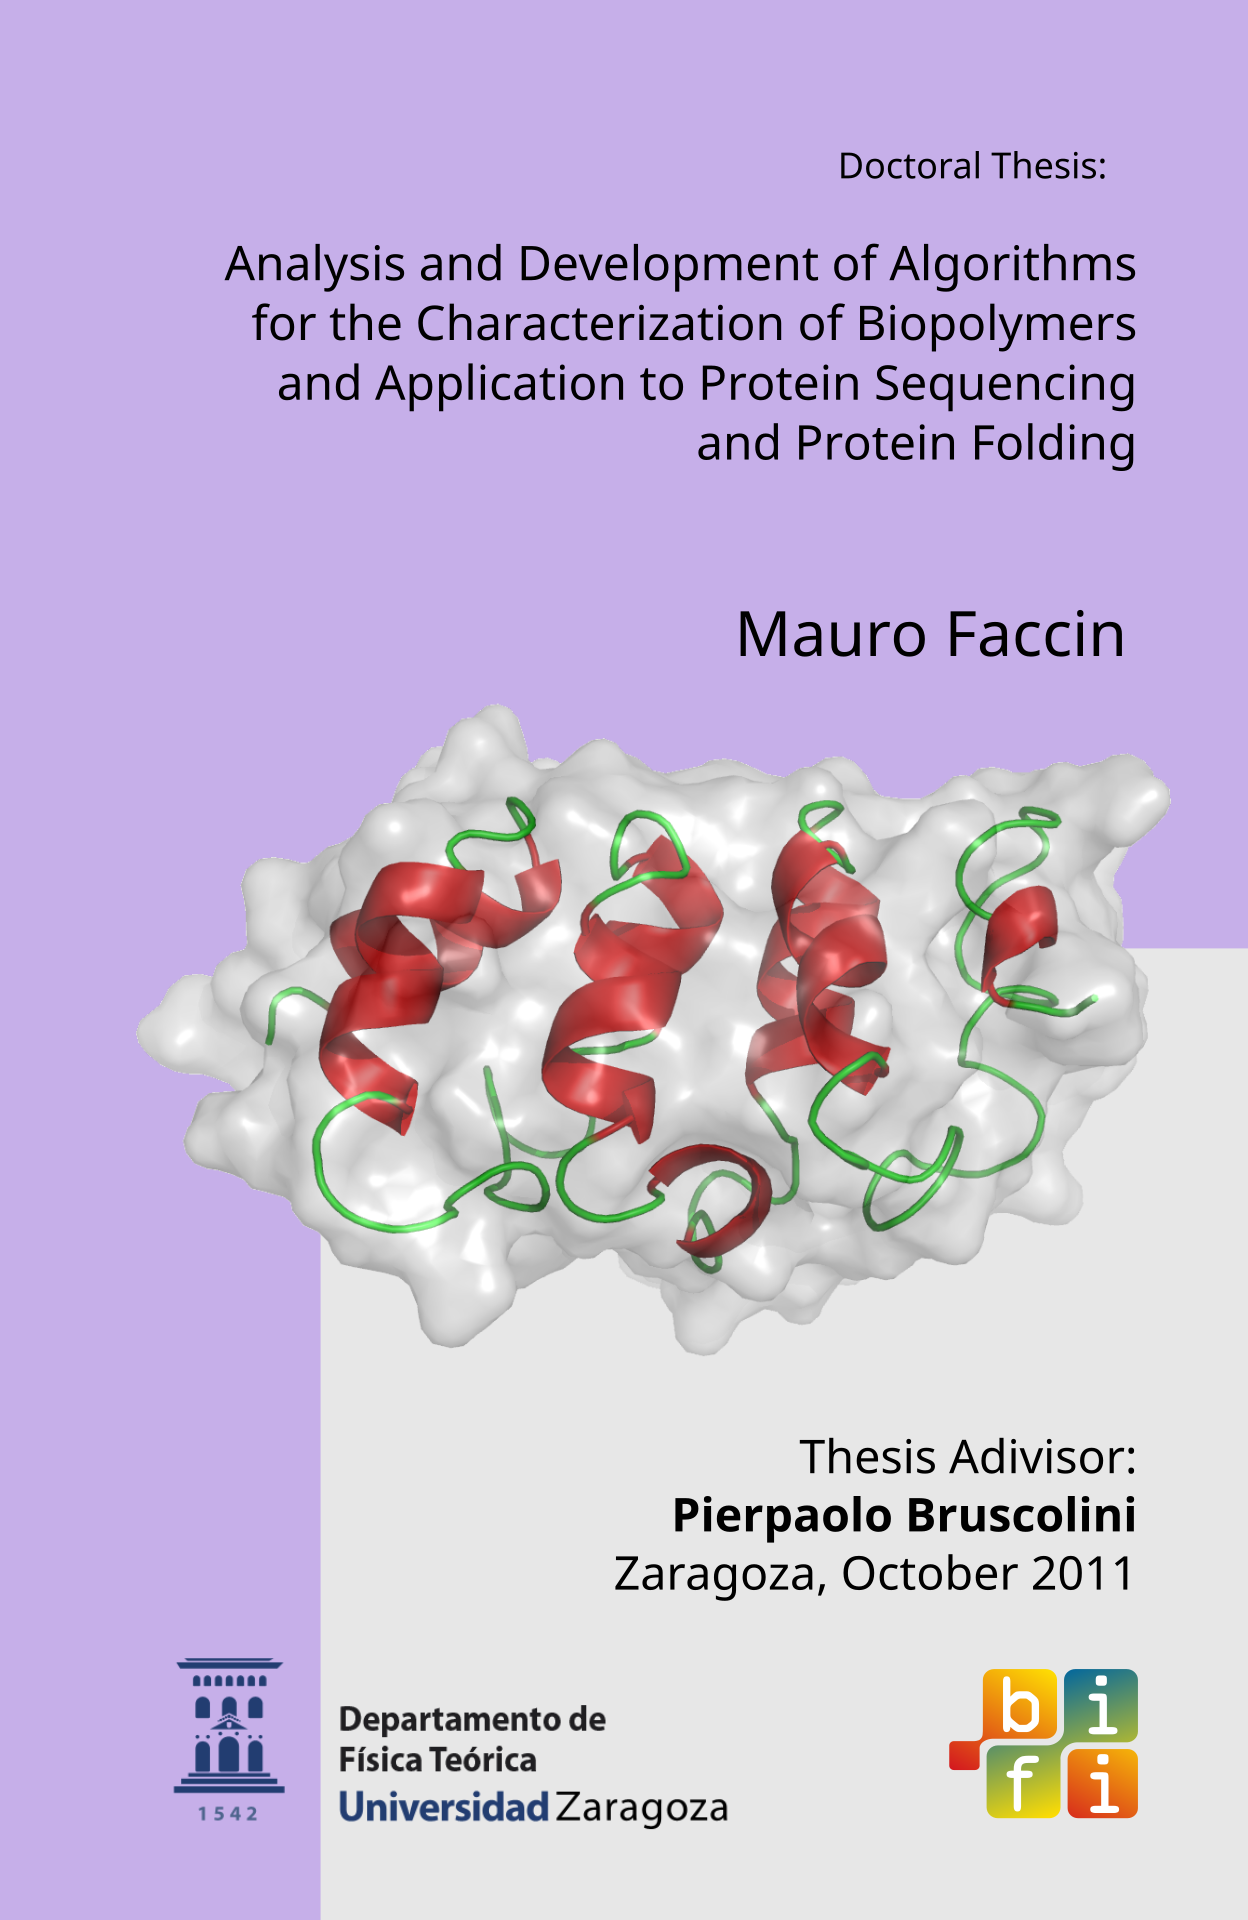
\includegraphics[width=1.001\paperwidth]{cover-front}
  };
  
\end{tikzpicture}

\cleardoublepage%

% ESTE DOCUMENTO GENERARA LAS PRIMERAS PAGINAS DEL LIBRO

% estas paginas las voy a numerar en romanos
\pagenumbering{roman}

\newcommand{\vquant}{\vskip 0.05\textheight}

\begin{titlepage}

\begin{flushright}
\rule{\linewidth}{0.5mm}\\
{\Large \bf 
Analysis and Development of Algorithms\\
for the Characterization of Biopolymers\\ 
and Application to Protein Sequencing\\
and Protein Folding.\\}
\rule{\linewidth}{0.5mm}\\
\end{flushright}

\begin{minipage}{\textwidth}
\centering

\vquant
\vquant
{\large \bf Mauro Faccin}

\vquant
\vquant
Departamento de F\'isica Te\'orica\\
Instituto de Biocomputac\'on y F\'isica de los Sistemas Complejos\\
\textsc{Universidad de Zaragoza}


\vquant
Tesis Dirigida por:\\
{\large \bf Pierpaolo Bruscolini}

\vquant
\vquant
Junio, 2011
\end{minipage}

\vfill
\begin{center}

\includegraphics[width=0.5\textwidth]{./img/loghi/logo-nuevo-unizar-bn.eps}
\end{center}
\end{titlepage}

\newpage
\thispagestyle{empty}
\ \\
\newpage

\thispagestyle{empty}\
\mbox{}
\newpage


%% AQUI LE DIGO QUE DEBE PONER EN LA CABECERA DEL INDICE:
\fancyhf{}
\fancyhead[LE,RO]{\small \rm \thepage}       % pages and right on odd pages%
\fancyhead[RE]{\small \sl Contents}   % Chapter in the right on even pages
\fancyhead[LO]{\small \sl Contents}   % Section in the left on odd pages
%% HECHO!!

\parskip 0cm
\tableofcontents 
\markboth{Contents}{Contents}
\parskip 0.2cm

%% AHORA LE TENGO QUE DECIR COMO HACER EL RESTO BIEN. EN LA SECCION DE
%% BILIBOGRAFIA NECESITARE HACER OTRO CAMBIO
\fancyhf{}
\fancyhead[LE,RO]{\small \rm \thepage}       % pages and right on odd pages%
\fancyhead[RE]{\small \sl \leftmark}      % Chapter in the right on even pages
\fancyhead[LO]{\small \sl \rightmark}     % Section in the left on odd pages
%

\cleardoublepage%

\pagenumbering{arabic}

%%%%%%%%%%%%%%%%%%%%%%%%%%%%%%%%%%%%%%%%%%%%%%%%%%%%%%%%%%%%
\chapternonum{Resumen}
\nopagebreak
%%%%%%%%%%%%%%%%%%%%%%%%%%%%%%%%%%%%%%%%%%%%%%%%%%%%%%%%%%%%




%\paragraph{} %senza questo non funziona il correttore ortografico nel resto
\lettrine{E}{l} estudio de esta Tesis se centra en de dos problemas
biológicos distintos aplicando un enfoque estadístico-mecánico común:
en el primer caso el trabajo se centra en el problema de la secuenciación de los
péptidos a través de la interpretación \emph{de novo} de espectros de masa
tándem, mientras que en el segundo se estudia el plegamiento de la Miotrofina,
una pequeña proteína de tipo modular que ha sido recientemente caracterizada por
diferentes técnicas experimentales.
 
Ambos problemas, como la mayoría de los problemas de tipo biológico, son
demasiado complejos como para ser tratados de una manera detallada, \emph{ab
initio}, basándose en una descripción microscópica de las interacciones y de
los procesos fundamentales involucrados; generalmente para poderlos tratar, se tiene que introducir
varias simplificaciones en el modelo del sistema original, a costa de
incluir, inevitablemente, ciertas aproximaciones.
El típico enfoque empleado en la descripción de sistemas biológicos desde un
punto de vista mecánico-estadístico se basa en la traducción efectiva del
sistema complejo original a un modelo físico tratable, posiblemente involucrando
el uso de coarse-graining u otros tipos de simplificaciones.

En el caso tratado en esta Tesis hemos reescrito el problema original mencionado antes, en
términos de un oportuno sistema mecánico estadístico a través de la definición
de las variables dinámicas interesantes y de una función energía que determina
su comportamiento.
Además en ambos problemas hemos forzado una modelización de las interacciones que
nos permita calcular una solución exacta de la distribución de probabilidad en el
equilibrio a través del método de la matriz de transferencia.

Ambos problemas están relacionados con proteínas: su identificación con MS/MS y su
plegamiento. 


%esta Tesis tratamos de caracterizar dos aparentemente distintos problemas
%biol\'ogicos: en el primer caso nos acercamos al problema del secuenciación de
%p\'eptidos en el campo de la Espectrometr\'ia de Masa, mientras en el segundo hemos
%analizado el plegamiento del la prote\'ina modular Miotrofina.
%La transformaci\'on de los problemas biol\'ogicos a un sistema mec\'anico estad\'istico
%se ha tratado con la definici\'on de las variables din\'amicas interesantes y con la
%escritura de una funci\'on conste que gobierna sus comportamientos.
%El sistema, si separable en subsistemas con interacciones solamente a primeros
%vecinos, ofrece una soluci\'on exacta por la distribuci\'on de probabilidad al
%equilibrio a trav\'es del mecanismo de la matriz de transferencia.
%En este estudio nos basamos en esta caracter\'istica para profundizar en la
%descripci\'on de estos sistemas y su diferentes conformaciones.

%\paragraph{¿Que son las Proteínas?}
%Las Proteínas son moléculas omnipresentes en las células, ellas son involucradas
%en la mayoría de los procesos bioquímicos que gobiernan su evolución.
%Las proteínas son polímeros compuestos por secuencias de aminoácidos, y cuya
%estructura puede ser descrita por medio de una sucesión de símbolos que componen
%un alfabeto de aminoácidos, esta sucesión se llama estructura primaria.
%La cadena de aminoácidos que compone la proteína se pliega generalmente en una
%dada, usualmente globular, estructura tridimensional, adquiriendo de esta forma
%la función bioquímica que tendrá que desempeñar.
%
%La síntesis de proteínas se lleva a cabo dentro de la célula a través de un
%mecanismo de traducción del ADN.
%La información de la composición en aminoácidos es, en efecto, codificada en la
%doble hélice del ADN. Éste se encuentra empaquetado en el nucleo de la célula
%donde, si hay demanda, se desempaqueta localmente para transcribir su contenido
%en un suporte temporal llamado ARN.  
%El ARN sale del núcleo de la célula y entra en el citoplasma donde se encuentran
%los Ribosomas, aquí el ARN puede someterse a algunas modificaciones antes de
%empezar la traducción a una cadena polipeptídica.
%Los Ribozomas descodifican el ARN mensajero usando unas reglas que asignan a
%cada tripleta de nucleótides del ARN un residuo especifico, este, entonces,
%es agregado a la cadena del péptido final.
%
%Una vez concluida la construcción de la cadena de aminoácidos, esta entra en el
%proceso de plegamiento para alcanzar la estructura tridimensional que le
%confiere su función bioquímica.
%A menudo a este estadio de la síntesis, la proteína puede subir unas
%modificaciones, caracterizadas sobre todo por agregación o perdida de grupos
%funcionales.
%
%Las proteínas se pliegan en una estructura estable, donde se encuentran a menudo
%unos patrones dominantes, sobre todo hélices $\alpha$ y hojas $\beta$, llamadas
%estructuras secundarias.
%Estos módulos se ordenan en la estructura terciaria global de la molécula
%plegada.
%Una estructura cuaternaria se puede encontrar en los complejos de proteínas
%ligadas entre si a formare una superestructura funcional.
%
%Las proteínas se pliegan de manera natural en las condiciones biológicas a las
%que son sometidas, experimentando un proceso de plegamiento fuera del
%equilibrio, desde una configuración priva de estructura, la proteína alcanza el
%estado nativo.
%El plegamiento es caracterizado por el camino seguido por el polímero en este
%proceso que describe la formación, dependiente del tiempo, de los contactos a
%largo alcance entre residuos no vecinos.
%El principal mecanismo de este proceso puede ser resumido en cuatro
%comportamientos principales\cite{Nickson2010}: 
%los módulos de estructura secundaria se forman primero, luego estos difunden y
%chocan hasta formar la estructura correcta; los residuos hidrófobos colapsa en
%centro como consecuencia del ambiente acuoso, provocando el plegamiento; un
%núcleo central empieza el proceso, propagándose luego a resto de la cadena; el
%núcleo de agregación no basta a provocar el plegamiento, este adviene cuando un
%numero critico de enlaces a largo alcance se hayan formado.
%
%La caracterización del camino de plegamiento se basa en la definición de los rasgos de
%cada conformación molecular antes de alcanzar el estado nativo\cite{Daggett2002}
%que refleja las características del paisaje energético.
%Esto ha sido alcanzado de manera satisfactoria solamente en proteínas pequeñas,
%combinando resultados experimentales con simulaciones de dinámica molecular.
%De otra parte, estudios experimentales de plegamiento de proteínas proporciona
%una instantánea de la estructura a lo largo del camino que, aunque no
%proporciona una información temporal de la formación de contactos, puede sugerir
%los atributos de los estados intermedios y del mecanismo general del proceso.

%%%%%%%%%%%%%%%%%%%%%%%%%%%%%%%%%%%%%%%%%%%%%%%%%%%%%%%%%%%%%%%%%%%%%%%%%%
\paragraph{Secuenciamiento de Prote\'inas}

En la primera parte de la Tesis afrontamos el problema de la secuenciación de
p\'eptidos en el marco de la Espectrometr\'ia de Masa, que consiste en la
interpretación de un espectro de masa para encontrar la secuencia de amino
ácidos del péptido estudiado.
Gracias a su simplicidad y bajo coste, el uso de esta herramienta se
utiliza ampliamente en el campo del análisis bioquímica de muestras
desconocidas de proteínas, y, generalmente, está incrustada en una
instrumentación de tipo high-throughput automatizada, que produce una gran
cantidad de datos, necesitando entonces una herramienta automatizada para
interpretarlos. 

En principio, un espectro de masa tándem contiene toda la información necesaria
para encontrar la secuencia de amino ácidos del péptido que generó el espectro mismo.
En la práctica, encontrar dicha secuencia desde un espectro es una tarea muy
difícil por la presencia de ruido, picos debidos a iones
contaminantes, o falta de fragmentaciones, entre otras cosas.
De echo, cada espectro es el resultado de las reglas microscópicas que gobiernan
la transferencia de energía y la fragmentación estocástica del péptido precursor
en las colisiones, en presencia de ruido y contaminantes de diferentes tipos.
Desafortunadamente, la predicción \emph{ab initio} del espectro resultante a
partir de la secuencia del péptido precursor es impracticable, si no imposible,
y la interpretación de la secuencia del péptido involucra el uso de funciones
coste \emph{ad hoc} para medir el acuerdo entre el espectro teórico de un
péptido precursor y el espectro experimental.
Además, el espacio de búsqueda de las secuencias es generalmente limitada a las
secuencias de proteínas ya conocidas (``búsqueda sobre bases de datos''). 
Gracias a esta restricción la búsqueda de la secuencia resulta
más practica y eficiente de los métodos \emph{de novo}
que infieren la secuencia del péptido a partir solo de la información contenida
en el espectro, pero está afectada por sus limitaciones.
Finalmente en ambos métodos es importante subrayar que un problema central es la
asignación de un ``grado de confianza'' a las predicciones, entre las cuales
se pueden encontrar falsos positivos, o sea secuencias equivocadas con alta
puntuación.


A continuación describimos un nuevo algoritmo basado en la traducción del problema de la
interpretación, al análisis de la distribución al equilibrio de un sistema
físico discreto adecuadamente definido, cuyas variables dinámicas describen la
presencia de un enlace peptídico (un sitio de fragmentación) en los nodos de un
retículo unidimensional, etiquetado por un índice de masa.
La función energía \emph{ad hoc} que gobierna el modelo, se deduce de la
distribución fenomenológica de los iones y de los picos de ruido en un conjunto de espectros
experimentales.
Las interacciones que caracterizan esta Hamiltoniana son interacciones locales o
a primeros vecinos de manera que la función de partición del modelo puede ser
calculada exactamente con el método de la matriz de transferencia.
Mientras que la identificación de la secuencia del péptido está asociada a la
caracterización del estado fundamental a temperatura cero, la introducción de
una temperatura paramétrica y el estudio de las variables termodinámicas como
función de la temperatura pueden dar una idea de la calidad de la
interpretación, sin apoyarse a bases de datos decoy (bases de datos compuestas por
secuencias equivocadas pero con alta puntuación) o en la distribución
fenomenológicas de las puntuaciones de los falsos positivos.

Aumentando la temperatura, el equilibrio del sistema se aleja
de un régimen dominado por la energía y polarizado hacía la secuencia mejor
puntuada, para alcanzar un régimen dominado por la entropía debida a otras
secuencias con una menor puntuación, lo cual puede ser útil para evaluar la bondad de la predicción.

El algoritmo ha sido testado sobre un conjunto de espectros experimentales 
acoplados con la secuencia teórica del péptido precursor y sobre el mismo
conjunto han sido testados algunos de los algoritmos \emph{de novo} disponibles
(NovoHMM, PepNovo, Lutefisk).
Nuestro algoritmo produce resultados comparables con los programas existentes
y además exhibe algunas características útiles relacionadas con el sistema 
termodinámico asociado que no se encuentran en los demás.
Sobresale como característica del algoritmo
la posibilidad de controlar la temperatura de trabajo que,
junto con la posibilidad de calcular exactamente la distribución de
probabilidad al equilibrio, proporciona la oportunidad de considerar al
mismo tiempo el entero espacio de las secuencias cada una con su ``peso''
termodinámico.

%%%%%%%%%%%%%%%%%%%%%%%%%%%%%%%%%%%%%%%%%%%%%%%%%%%%%%%%%%%%%%%%%%%%%%%%%%%%%%
\paragraph{Plegamiento de la Prote\'ina Miotrofina}
En la segunda parte de la Tesis nos hemos centrado en el problema del
plegamiento del las proteínas, tratando de caracterizar en particular el
equilibrio y la cinética de la Miotrofina, una proteína de tipo modular.
El plegamiento de proteínas es un problema que ha sido enormemente estudiado y
analizado por parte de los teóricos a partir de muchos niveles de
coarse-graining, empezando por
las simulaciones a todos los átomos con interacciones realistas, a una variedad
de modelos de coarse-graining.

La proteína estudiada en este trabajo, la Miotrofina, es una proteína modular
compuesta por cuatro módulos con la misma estructura secundaria aunque
diferentes secuencias, dispuestos en una conformación lineal.
Esta conformación, común a las proteínas modulares, las diferencia de las ampliamente estudiadas
proteínas globulares. 
En las proteínas globulares las
regiones alejadas en la secuencia se acercan y entran en ``contacto'' cuando la
proteína se encuentra en el estado nativo, y el alcance de los contactos puede
abarcar la entera molécula.
En las proteínas modulares solo hay contactos dentro de cada
módulo y entre amino ácidos pertenecientes a módulos contiguos.
La Miotrofina muestra un comportamiento interesante que ha atraído la atención
de los investigadores: la molécula parece plegarse de manera cooperativa,
característica típica de las proteínas globulares, mientras su estructura
modular sugiere una independencia intrínseca de cada módulo, naturalmente
asociado a un plegamiento con varios estados
intermedios que corresponden al plegamiento independiente de los módulos.


En este trabajo nos basamos en el modelo propuesto por Wako- Saito-Mu\~noz-Eaton
(WSME) 
para caracterizar el plegamiento de la Miotrofina.
Este simple modelo se basa en el uso de una variable binaria para describir el estado
(``plegado'' o ``desnaturalizado'') de cada residuo usando la información
contenida en la estructura nativa de la molécula, la cual está almacenada en un mapa de
contactos que describe la proximidad euclídea de dos residuos y de esta forma predecir el
comportamiento en el proceso de plegamiento.
A pesar de la presencia de interacciones a largo alcance, la forma especial de la función energía
del modelo, le otorga la posibilidad de evaluar exactamente la
función de partición, así como las cantidades termodinámicas en el equilibrio, como
la energía libre y la capacidad calorífica, mientras que para describir la dinámica
del sistema hay que usar unas simulaciones de tipo Monte Carlo.

Usamos el modelo WSME para estudiar la molécula wild-type como algunas
mutaciones y por esto tratamos las mutaciones puntuales como variaciones del potencial
de interacción del residuo interesado.

En ambos casos, los resultados muestran un buen acuerdo con los datos
experimentales, haciendo particular hincapié en la heterogeneidad de los caminos de
plegamiento.
El minucioso control sobre las simulaciones, que sobrepasa las posibilidades
experimentales, nos otorga la posibilidad de sugerir las caracter\'isticas de los
procesos subyacentes, entre ellos sobresale el acuerdo entre la estructura modular, 
que produce un
perfil de la energía libre con múltiple mínimos, y la cooperaci\'on en el proceso
de plegamiento, y además sobresale que la simetr\'ia entre los caminos de
plegamiento y de desnaturalizaci\'on de la mol\'ecula no es una condición necesaria.




%%%%%%%%%%%%%%%%%%%%%%%%%%%%%%%%%%%%%%%%%%%%%%%%%%%%%%%%%%%%
\chapternonum{Introduction}
\nopagebreak
%%%%%%%%%%%%%%%%%%%%%%%%%%%%%%%%%%%%%%%%%%%%%%%%%%%%%%%%%%%%

%%%%%%%% Quote
%\begin{flushright}
%\parbox[h]{4.in}{{\small{\em 
%%The greatest challenge today, not just in cell biology and ecology but in all
%%of science, is the accurate and complete description of complex
%%systems. Scientist have broken down many kinds of systems. They think they
%%know most of the elements and forces. The next task is to reassemble them, at
%%least in mathematical models that capture the key properties of the entire ensembles
%
%Professor Hubert Farnsworth: Good Lord! That's over 5000 atmospheres of pressure!\\
%Fry: How many atmospheres can the ship withstand?\\
%Professor Hubert Farnsworth: Well, it was built for space travel, so anywhere between zero and one.\\
%\ \\ 
%Ludwig Boltzmann, who spent much of his life studying statistical mechanics,
%dies in 1906, by his own hand.\\
%Paul Ehrenfest, carrying on the work, died similarly in 1933.\\
%Now it's our turn to study statistical mechanics. Perhaps it will be wise to approach
%the subject cautiously.\\
%David Goodstein - \emph{State of Matter}, 1975, Dover N.Y.
%}}
%%\begin{flushright}
%%{\small Edward O. Wilson \cite{Wilson}.}
%%\end{flushright}
%}
%\end{flushright}


\paragraph{} %senza questo non funziona il correttore ortografico nel resto
\lettrine{T}{his} Thesis 
% focus on the application of the tools of
% Statistical Mechanics to the study and analysis of two different and relevant problems in modern molecular biology: 
% %biological systems. In particular we will focus in  
% the problem of protein sequencing by mass spectrometry and the  problem of 
% protein folding, with a special focus on the study of a modular protein.
% %in particular  of in the case of modular polymers.
addresses
%attempt to characterize 
two different %apparently unlike 
biological
problems with a common statistical-mechanics approach: in the first case we focus
on the problem of peptide
sequencing by {\sl de-novo} interpretation of Tandem %in the field of 
Mass spectra, while in the second we 
analyse the folding behaviour of Myotrophin, a small repeat protein that has been recently characterized by different experimental techniques.

Both problems, as the majority of  biologically relevant systems and processes,
are too complex to be approached in a detailed, \emph{ab-initio} way, based on a
reliable, microscopic description of the interactions and fundamental processes
involved; on the contrary, typically 
% Actually the majority of the biological interesting processes are too complex
% for a deep study based in its fundamental constituents and the driving forces acting
% on them, in exchange 
one has to resort to  %rely on 
various simplifications in the modelling of the original system, introducing, as
a consequence,  some approximations in order to achieve treatability. 
Hence,  the typical approach to the description of a biological system from a statistical-mechanics %physical
point of view starts with the research of a successful mapping of the
original complex problem to a treatable physical model, possibly involving coarse-graining or other kind of simplifications. 
%usually based on statistical mechanics, at different levels of details retain. 


In our case, the mapping of the above mentioned problems to 
%The map of each of those cases to a 
suitable statistical mechanical systems is performed
through the definition of the interesting dynamic variables and of an
energy function which determines their behaviour.
Moreover, for both problems we enforce a modelling of the interactions that 
% The resulting system, if breakable in subsystems that present interaction only
% with first neighbours, 
is amenable of an exact solution for the equilibrium
probability distribution through the Transfer Matrix Method.

Both problems are related to proteins: their identification with MS/MS and their folding. In the following, we resume some basic facts about such important biomolecules: their synthesis, their structure and their role in cellular processes.
% In the following we rely on this characteristic to take an insight in the system
% behaviour and its different conformations.

\paragraph{What is a Protein?}
Proteins are ubiquitous molecules in living cells, involved in almost all the
biochemical processes that govern their evolution.
Proteins are linear polymeric  chains,
composed by different combinations of 20 types of amino acids, covalently linked  in a sequence (the ``primary structure'') that completely encodes their three-dimensional structure and function. 
Each protein is completely characterized by its sequence, whose length may vary
between a few tens to several hundred ``residues'', as the amino acids are
called within the protein chain (the name acknowledges the fact that  they loose
a water molecule upon binding in the main chain).
% 
% This long chain of residues folds usually to a given, usually globular,
% three-dimensional structure, acquiring a functional role.

Protein synthesis is performed inside the cell through a DNA translation
mechanism,  based on the information contained in  the regions of the chromosomes corresponding to the genes.
The information on protein composition is, in fact, encoded into the DNA double
helix. The latter is found packed in the cell nucleus and is locally unpacked
``on demand'' and copied to a messenger mRNA strand (DNA transcription).
The mRNA strand exits the nucleus to reach the cytoplasm where the ribosomes are
located;  here, it can
undergo some modification (removal of the introns, alternative splicing) before being translated to a polypeptide chain.
Ribosomes decode the messenger RNA using the tri-nucleotide translation rules, that assign to each triplet
of RNA basis (``codons'') a specific residue to be appended to the peptide chain.

Once the amino acid chain is built up, it undergoes the process of folding to reach
its functional three-dimensional structure (the ``native structure''), which  is usually a precisely determined compact structure.
Often at this stage  the  newly formed protein undergoes some modification, mainly
characterized by the addiction of functional groups to polypeptide chain.
Notice that these changes cannot be read from the genetic code of the DNA, and depend on the specific cell conditions at the moment the protein is synthesized. 


\begin{figure}
\centering
\def\svgwidth{0.8\textwidth}
%% Creator: Inkscape inkscape 0.48.2, www.inkscape.org
%% PDF/EPS/PS + LaTeX output extension by Johan Engelen, 2010
%% Accompanies image file 'dna-transcription-translation-divided-text.eps' (pdf, eps, ps)
%%
%% To include the image in your LaTeX document, write
%%   \input{<filename>.pdf_tex}
%%  instead of
%%   \includegraphics{<filename>.pdf}
%% To scale the image, write
%%   \def\svgwidth{<desired width>}
%%   \input{<filename>.pdf_tex}
%%  instead of
%%   \includegraphics[width=<desired width>]{<filename>.pdf}
%%
%% Images with a different path to the parent latex file can
%% be accessed with the `import' package (which may need to be
%% installed) using
%%   \usepackage{import}
%% in the preamble, and then including the image with
%%   \import{<path to file>}{<filename>.pdf_tex}
%% Alternatively, one can specify
%%   \graphicspath{{<path to file>/}}
%% 
%% For more information, please see info/svg-inkscape on CTAN:
%%   http://tug.ctan.org/tex-archive/info/svg-inkscape
%%
\begingroup%
  \makeatletter%
  \providecommand\color[2][]{%
    \errmessage{(Inkscape) Color is used for the text in Inkscape, but the package 'color.sty' is not loaded}%
    \renewcommand\color[2][]{}%
  }%
  \providecommand\transparent[1]{%
    \errmessage{(Inkscape) Transparency is used (non-zero) for the text in Inkscape, but the package 'transparent.sty' is not loaded}%
    \renewcommand\transparent[1]{}%
  }%
  \providecommand\rotatebox[2]{#2}%
  \ifx\svgwidth\undefined%
    \setlength{\unitlength}{522.10136108bp}%
    \ifx\svgscale\undefined%
      \relax%
    \else%
      \setlength{\unitlength}{\unitlength * \real{\svgscale}}%
    \fi%
  \else%
    \setlength{\unitlength}{\svgwidth}%
  \fi%
  \global\let\svgwidth\undefined%
  \global\let\svgscale\undefined%
  \makeatother%
%  \begin{picture}(1,0.36337107)%
  \begin{picture}(1,0.37)%
    \put(0,0){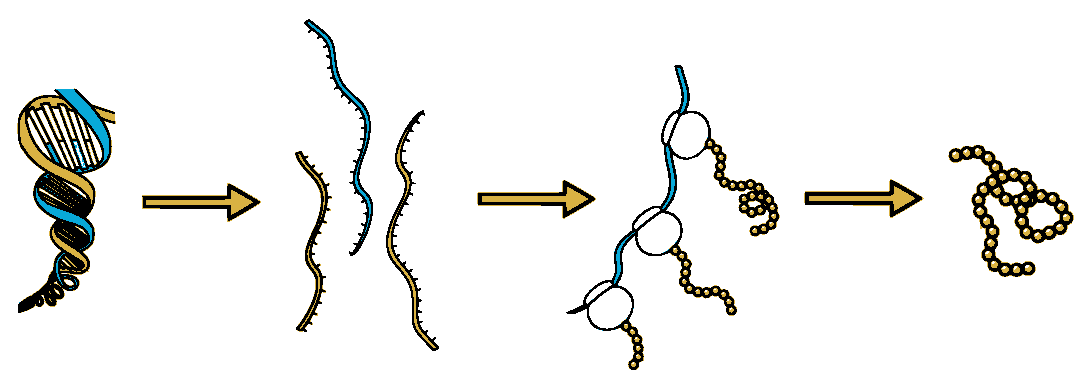
\includegraphics[width=\unitlength]{./img/msms/dna-transcription-translation-divided-text.eps}}%
    \put(0.05002023,0.33543109){\color[rgb]{0,0,0}\makebox(0,0)[lb]{\smash{Transcription}}}%
    \put(0.55348021,0.33543109){\color[rgb]{0,0,0}\makebox(0,0)[lb]{\smash{Traduction}}}%
%    \put(-0.00360921,0.00052073){\color[rgb]{0,0,0}\makebox(0,0)[lb]{\smash{DNA}}}%
%    \put(0.2820496,0.00052073){\color[rgb]{0,0,0}\makebox(0,0)[lb]{\smash{RNA}}}%
%    \put(0.53268515,0.00052073){\color[rgb]{0,0,0}\makebox(0,0)[lb]{\smash{Ribosomes}}}%
%    \put(0.87416237,0.00052073){\color[rgb]{0,0,0}\makebox(0,0)[lb]{\smash{Protein}}}%
    \put(-0.00360921,0.0005){\color[rgb]{0,0,0}\makebox(0,0)[lb]{\smash{DNA}}}%
    \put(0.2820496,0.0005){\color[rgb]{0,0,0}\makebox(0,0)[lb]{\smash{RNA}}}%
    \put(0.53268515,0.0005){\color[rgb]{0,0,0}\makebox(0,0)[lb]{\smash{Ribosomes}}}%
    \put(0.87416237,0.0005){\color[rgb]{0,0,0}\makebox(0,0)[lb]{\smash{Protein}}}%
  \end{picture}%
\endgroup%

%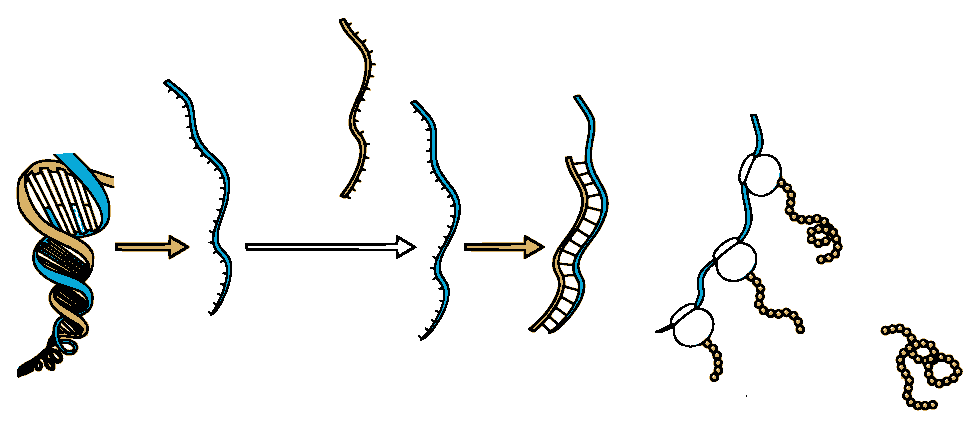
\includegraphics[width=0.7\textwidth]{./img/msms/dna-transcription-translation.eps}
\caption{Schematic representation of the DNA transcription and translation
processes. The information coded in the DNA is transcripted into an messenger
RNA to exit the nucleus where it is stored. Once in the cytoplasm the mRNA is
decoded by ribosomes, the latter assign to each nucleotide triplet a specific
residue, conforming the final polymeric structure of the protein.}
\end{figure}

Proteins fold in stable structures, dominated by
recurring structural motifs, mainly $\alpha$-helices and $\beta$-sheets,
called ``secondary structures''.  
The local regularity of these motifs is related to the strong directionality  of the hydrogen bonds that dictate their geometry.
These motifs are arranged in the global tertiary structure of the folded molecule.
A quaternary structure is defined by proteins complexes where several proteins
are arranged in a functional superstructure.
The above ``structural paradigm'' applies to all proteins with the exception of
the Intrinsically Unfolded Proteins, that are functional in a disordered
conformation; however, such proteins usually get structured upon binding to
their target molecule, so that  we can say that the sequence-structure-function
relationship is still valid, in a loose sense.

\begin{figure}
\begin{center}
\subfigure[primary structure]{
\begin{minipage}{0.3\textwidth}
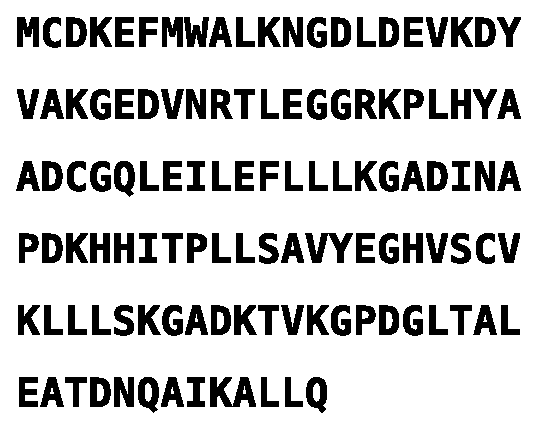
\includegraphics[width=\textwidth]{./img/2myo-seq.eps}\\
\vskip 5pt
\end{minipage}}
\subfigure[secondary structures]{
\begin{minipage}{0.3\textwidth}
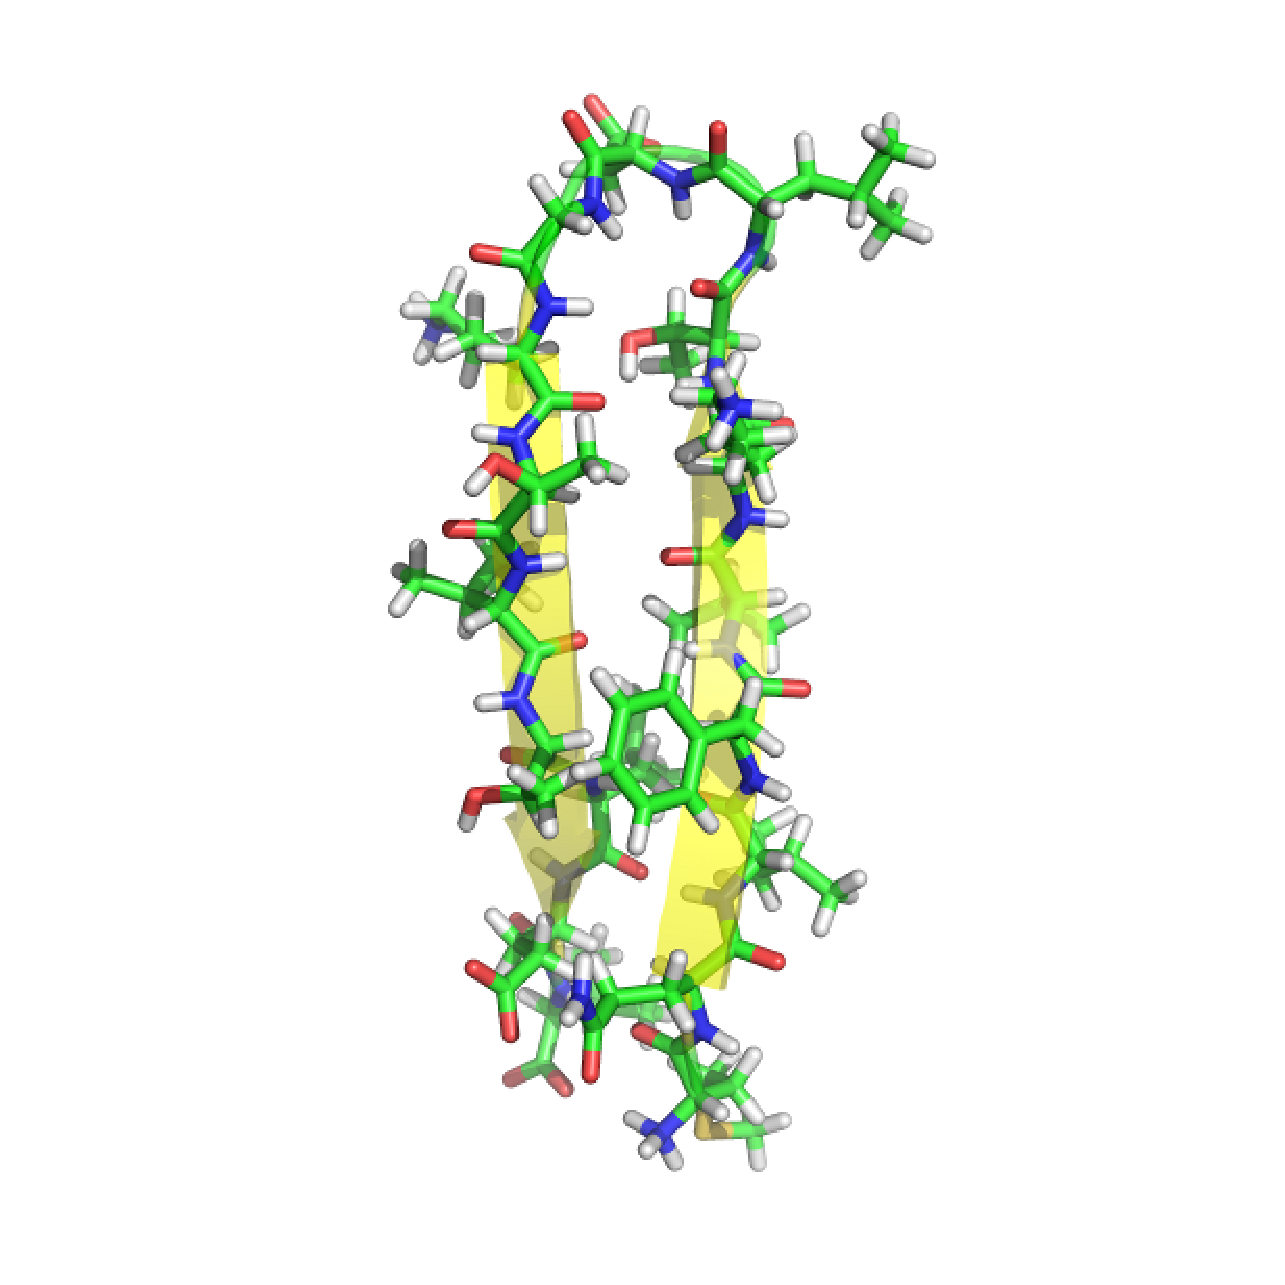
\includegraphics[width=\textwidth]{./img/1e0q-600.eps}\\
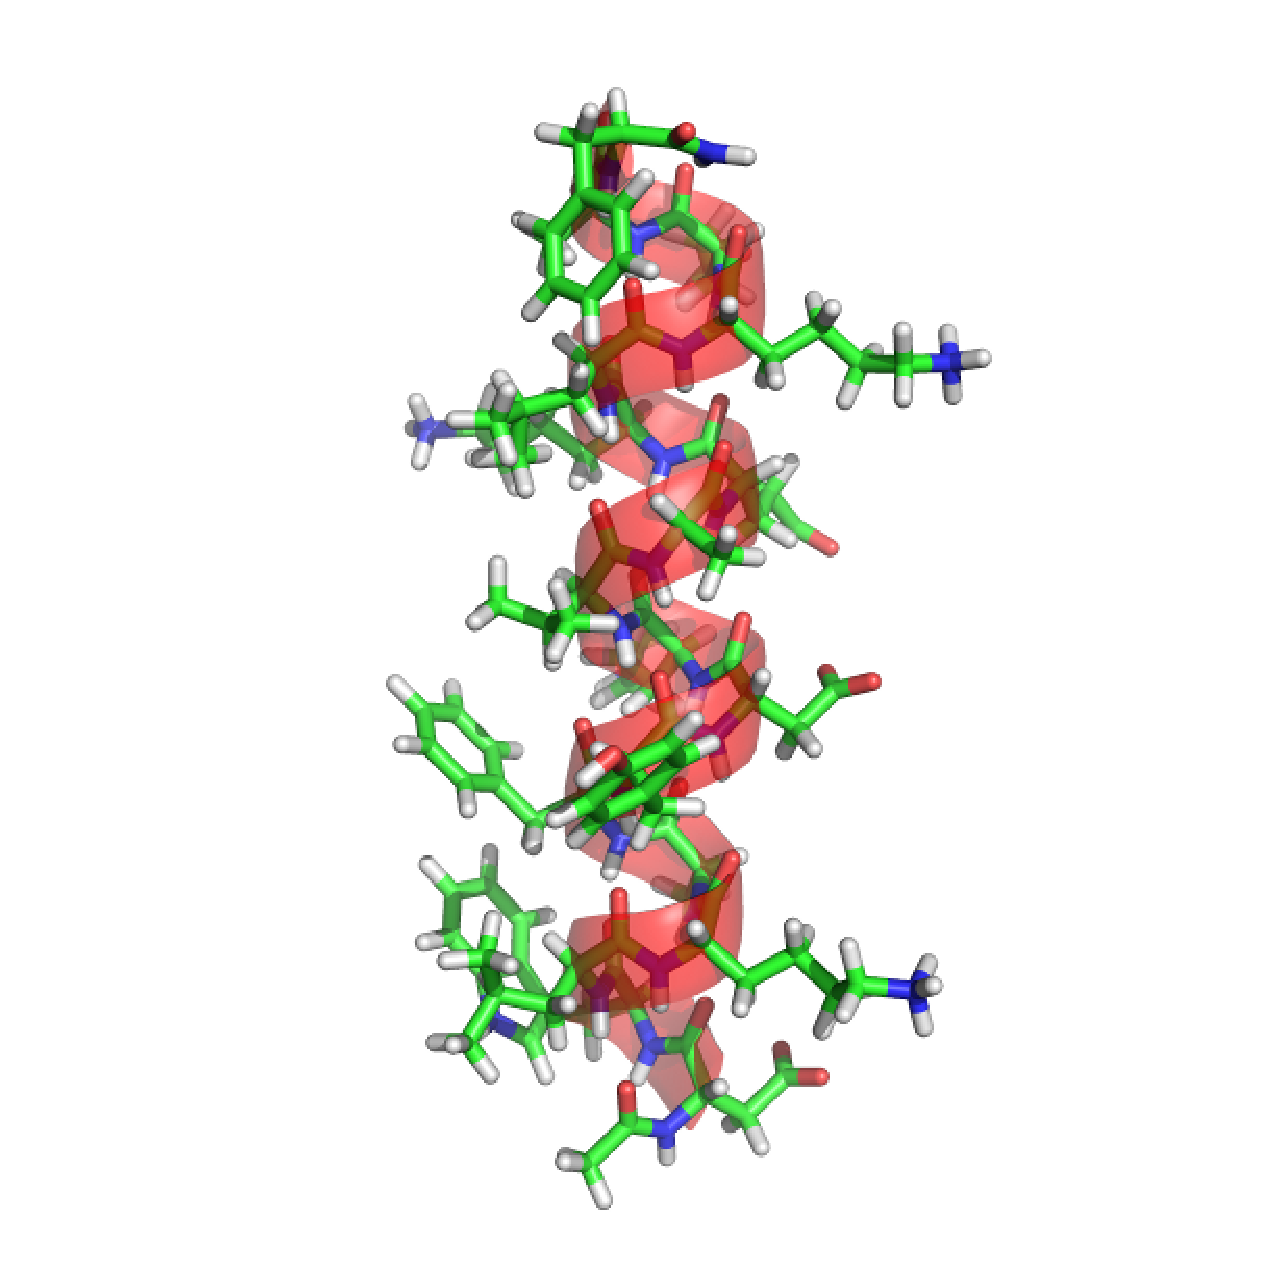
\includegraphics[width=\textwidth]{./img/2fq8-600.eps}
\end{minipage}}
\subfigure[tertiary structure]{
\begin{minipage}{0.3\textwidth}
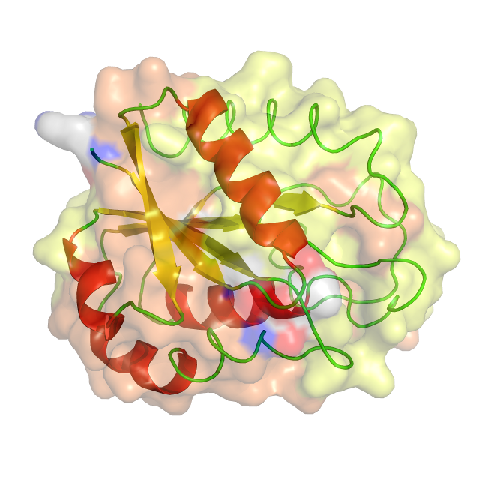
\includegraphics[width=\textwidth]{./img/1flv-600.eps}
\end{minipage}}
\end{center}
\caption{\label{fig:prot-structures}
The polymeric chain of a protein is determined by (a) the residue sequence.
The resulting chain naturally tends to assume a compact structure mainly
conforming (b) structural motifs such as  $\alpha$-helices and
$\beta$-sheets that are arranged on the final (c) native structure.}
\end{figure}

Proteins folds naturally in biological conditions, experiencing an
out-of-equilibrium process that, starting from an unstructured
configuration, ends on the folded native state. 
On the other hand, folding can be studied in vitro under equilibrium and our of
equilibrium conditions: 
from a thermodynamic point of view, the protein native state, in physiological
conditions, represents the stable macro-state, with minimal free-energy; a sudden change to different conditions results in a chemical kinetics that can be usually related to the final free-energy landscape,  and is characterized by the search of the most convenient pathway to reach the new equilibrium. 
In this sense, a folding pathway is specified in terms of the 
% Protein folding is characterized by the pathway followed by the polymer in this process as it describes the 
time dependent formation of the
long-range contacts between non-neighbouring  residues. 

The principal folding  mechanisms that have been identified can be summarized  in
four main behaviours \cite{Nickson2010}: a) Diffusion-Collision: secondary structure folds first and then
the motif diffuse and collide to form the correct structure; b) Hydrophobic Collapse:  
%hydrophobic residues collapse together 
due to the wet environment triggering the folding
process, the protein collapses to a molten globule to protect the non-polar residues from the polar solvent, then the search for the right structure is restricted to compact conformations; c) Nucleation-Propagation: a local nucleus starts the folding process and then propagates to
the entire structure; d) Nucleation-Condensation: the folding nucleus is composed of non-local contacts, involving distant residues along the chain; once a critical number of such contacts is formed, it triggers  the completion of the folding
process. % until it reach a critical number of formed long range contacts.

Different proteins, or even the same protein under different conditions, can show different folding mechanisms.
The detailed characterization of protein folding pathways passes through the
characterization of every conformation that the molecule assumes along the way to the
native state\cite{Daggett2002} and  reflects the picture of the energy landscape. Such characterization  has been successfully achieved  in small proteins combining experimental results with molecular dynamic
simulations: most often, the former 
%However experimental studies of protein folding 
provide snapshots of the
structures along the folding pathway that, although devoid of %they do not provide 
the temporal information on contact formation, can give a picture of the intermediate states
and the overall folding mechanism for the process, while the latter can give insight on the microscopic details of the relevant structures along the folding pathway. 



\paragraph{Protein Sequencing}
In the first part of the Thesis we focus on the problem of peptide
sequencing by Tandem  Mass Spectrometry, which consists in  the interpretation of a mass
spectrum to find the amino-acid sequence  of a target peptide.
Tandem Mass Spectrometry, thanks to its simplicity and low cost, is vastly used in the field of biochemical analysis of unknown
samples of protein, and is 
generally embedded in an automated high-throughput pipeline, which produces a huge
amount of data,  requiring an automated interpretation tool.

In principle,  a Tandem Mass spectrum contains all  the necessary information to find
the peptide sequence it comes from. In practice, reading out the sequence from the spectrum is always a difficult task, complicated by the presence of noise, of peaks from contaminants, and of missing or unexpected fragmentations.  
Actually, each spectrum is the statistical outcome of  the microscopic rules
governing the energy transfer and stochastic fragmentation of the precursor
peptide under collisions, in the presence of contaminants and of noise of
different kind.  Unfortunately, ab-initio predictions of the spectrum given a
precursor ion are  impractical, if not impossible,  and  the identification of
the peptide sequence involves the use of ad-hoc score functions to rate the
agreement between the  theoretical spectrum of a parent peptide and the
experimental one.  Moreover, the search space is usually limited to the
sequences of  known proteins (``database search'' approach), which is more
practical and efficient, but also more limited than de-novo methods which infer
the peptide from just the information contained in the spectrum. 
Finally, it is remarkable that, both for database-search and for de-novo
methods, a central problem is related to assessing the reliability of the
prediction, mainly related to the prediction of  false positives, i.e., wrong
sequences with high scores.

We describe a new algorithm for  protein sequencing based on the mapping of the
interpretation problem onto the analysis of the equilibrium distribution of a
suitably defined discrete physical model, whose dynamic variables describe the
presence of a peptide bond (a fragmentation site) on the sites of a
one-dimensional lattice, labelled by a mass index.
The model is governed by an \emph{ad hoc} energy function,  learned from the
distribution of the ions and of the noise peaks on a dataset of
experimental spectra.  Such Hamiltonian is characterized by just on-site and
nearest-neighbour interactions, so that the partition function of the model can
be exactly calculated by a transfer-matrix approach. While the identification of
the precursor peptide is associated to the characterization of the ground-state
of the model (the zero-temperature solution),
the introduction of a parametric temperature, which represents an original
approach to this problem, and the study of the thermodynamic variables as a
function of the temperature, can give insight on the quality of the
identification, without relying on decoy databases or on phenomenological
distribution of the scores of the false positives.
Indeed, as the temperature increases, the thermodynamic equilibrium shifts from
a regime dominated by the energy and polarized on the best scoring peptide
sequence, to a regime dominated by the entropy coming from  the alternative
sequences with a reasonably good  score on the experimental spectrum.

The resulting algorithm has been applied to a test database of spectra and the results are
reported in this thesis. We show that the performance of this algorithm is
comparable of existing and more popular models, while presents a new valuable
feature: the fictitious temperature that pulls the system outside the energetic
minimum can give the user a tool to estimate the quality of the prediction.


\paragraph{Protein Folding}
In the second part of the Thesis we deal with  the protein folding problem,
focusing in particular on  the characterization of the equilibrium and kinetics
of the repeat protein Myotrophin.
Protein folding is a challenging problem that has been vastly analysed by
theoreticians %physicists and chemists 
using different levels of coarse-graining, % with a wide range of levels of details, 
from all atoms simulations
with realistic interactions, to a variety of coarse grained models.

The protein studied in this work, Myotrophin, is a repeat protein composed by
four modules with the same secondary structure (but different sequence), %composition, 
arranged in a linear way. This kind of structural organization, common to all
repeat proteins,  makes them different from the commonly  studied globular
proteins: in the latter, far apart regions of the sequence can come close (``in
contact'') to one another in the native structure, and the contact range can
span the whole sequence length. On the contrary, in the former, contacts take
place just within a module and between contiguous modules.
Myotrophin
%This conformation experimentally 
shows a challenging behaviour, that has attracted  the attention of the researchers, as the molecule
seems to fold in a cooperative way, which is more typical of a globular protein, while %despite 
its modularity would suggest an intrinsic independence of the conforming
modules, more naturally associated to a multi-state folding, with several
intermediate states corresponding to the folding of independent modules.
Moreover, the experimental results on kinetics have been interpreted in the
framework of the existence of  two alternative folding pathways, labelled
according to which of the two protein ends folds first.

In this work we rely on the Wako- Saito-Mu\~noz-Eaton (WSME) model to characterize the behaviour of
Myotrophin.
This simple model resorts to a binary variable to describe the state (``folded'' or ``unfolded'') of each
residue, and uses the information on the atomic coordinates of the native %the wild type folded 
structure of a protein, stored in a contact map that describes the euclidean proximity of two residues,   to predict its folding behaviour. %describe the global and local behaviour of the polymer through the definition of 
Despite the presence of long-range  interactions  in the energy function of the model, its special form allows the exact evaluation of the partition function, so that equilibrium thermodynamic quantities such as free-energies and heat capacities can be exactly and efficiently calculated, while the dynamics can be studied by Monte Carlo simulations.

We use a slightly modified WSME model to study both the wild type protein and
some mutants; to this purpose, we mimic  single point mutations by changing the
interactions potentials of the mutated residue.
We introduce a new way to characterize, in the folding and unfolding processes,
the relaxation pathways based on the secondary structure formation and denaturation.

 
% of the wild type and qualitatively reproduce the general behaviour of the experimental data.

In both the wild type and mutant proteins, results show a good qualitative agreement with experimental results, with
particular emphasis on the heterogeneity of the folding pathways.
The higher control allowed by  \emph{in silico} simulations over \emph{in vitro}
experiments, and an original way to interpret kinetic data,
 let us shed some light on the subtending processes as the
consistency of the modular structure and free-energy profile and the folding
cooperativity, as well as the lack of  symmetry between the folding and
unfolding pathways.






%%%%%%% FIRST PART - MSMS
\part{De Novo Interpretation of Tandem Mass Spectra}

%%\begin{flushright}
%%\parbox[h]{4in}{\small\em
%%Thermodynamics is a funny subject.\\
%%The first time you go 
%%through it, you don't understand it at all.\\
%%The second time you go 
%%through it, you think you understand it, except for one or two 
%%small points. \\
%%The third time you go through it, you know you 
%%don't understand it, but by that time you are so used to it, it 
%%doesn't bother you anymore.
%%\begin{flushright} Arnold Sommerfeld.\end{flushright}
%%}
%%\end{flushright}

\sectionnonum{Introduction to the Problem}
\thispagestyle{plain}

\lettrine{T}{he} first part of the thesis deals with the application of
statistical mechanics methods to the interpretation of the experimental spectra
obtained with the Tandem Mass Spectrometry technique (usually abbreviated as
MS/MS, or MS2). The interest for the subject is two-fold: from a purely
theoretical point of view, we will show that the problem of the interpretation
of noisy MS/MS spectra can be mapped on the search for the equilibrium
distribution of the states of a suitably-designed one-dimensional lattice
system. The latter can be solved exactly, by a transfer-matrix technique, under
some approximations that we will discuss in Chapters \ref{chap:alg}. 
On the other hand, MS/MS spectra interpretation is nowadays  a key step 
%one of the main experimental techniques involved 
in high-throughput peptide and protein sequencing, a central subject in many
proteomics studies, with important implications also for genomics and
metabolomics.  To provide  the reader with a better understanding of the
relevance of the experimental technique, in the following we give an overview of
the application of MS/MS to proteomics.

Even if several definitions have been proposed, we can simply say that
proteomics is the study of the proteome of an organism: that is, the
identification of all possible protein contents of a cell, and their
characterization in terms of quantity, structure, function, and molecular
interactions. 

Proteomics arises as the ``natural'' counterpart, in the protein domain, of
genomics, that studies the genetic information of an organism.
Indeed,  sometimes the proteome has been simply identified as the protein
expression of the genome\cite{wilkins1996b,hochstrasser1998}. This view  is due
to the fact that the entire information, characterizing
the biochemical processes of any living system, is supposed 
to lay inside the genetic code; moreover, it is also fostered by the  enormous
growth of genetic data that have been collected in recent years, with the
complete decoding of the genomes of several organisms.

However, the above view is somewhat restrictive and incomplete, since it
suggests that protein content is
univocally defined from the genetic code, and a direct map can be performed
between genome and proteome.
In reality the information coded in the DNA undergoes several levels 
of modifications until it reaches the final state of usable protein.
During DNA transcription, information coded into DNA is copied to the mRNA,
which, in eukaryotes, can
undergo some post-transcriptional modifications  and intron splicing.
Moreover, the protein, obtained upon the translation of mRNA often undergoes 
some post-translational modifications, mainly consisting in the addition of cofactors
or  small chemical groups, which are related to its function.

This transcription-translation-modification process, in turn, is controlled by
the type and amount of the proteins and signalling molecules that are present in
the cell, providing a complex feedback mechanism that regulates any cell
activity. As a result,
the proteome of any organism is highly dynamic and changes over time; the types of
expressed proteins, their abundance, state of modification, sub-cellular location,
etc. depend on the physiological state of the cell, on the cell location
and on the tissue the cell belongs to, thus modifying and
giving a inherent and time-dependent structure to the static, overall
information that can be obtained by simply translating the genes into protein
sequences.

Needless to say, accessing the dynamical information on the changing protein
content of a cell is even more important that the static knowledge of its
genetic information, to shed light on how a cell functions at the molecular
level, how it reacts to adjust to external conditions, how we can distinguish  a
tumor cell from a normal one, just to mention a few possible questions.


For the above reasons, a fundamental goal in proteomics is represented by the complete
analysis of the protein content of a given sample, and answering a number of qualitative and
quantitative questions about the cell-sample content.
%It {\bf studies }
%provides information on the actual protein content as on the expression of the
%single proteins at a certain moment. 
%
%It can be used to study different cell
%events such as post translational modifications (PTMs) or protein mutation.
%It will be useful in phylogenetic investigations and...?????
Such analysis begins with the identification of the proteins expressed in a
cell, together with the post-translational modifications they carry: the latter
can provide important information, that cannot be read from the genome, on the
biological processes in which the protein is involved.

Several methods can be used to identify proteins, depending on the degree of
previous knowledge available: if the question is to find out if a known protein
is present in a mixture of a few proteins, low resolution techniques can be
sufficient,  consisting in a purification step to isolate the protein of
interest from the rest (for instance, by gel electrophoresis or mass
spectrometry), plus an identification test probing its interaction with a
suitable substrate (for instance, using antibody probes, as in Western Blotting
or ELISA tests).

Another intermediate resolution technique is protein fingerprinting, consisting
in cutting the protein of interest, proceeding from of a certain organism, into
smaller peptides, with some specific enzyme acting in a known way (for instance,
cleaving at every occurrence of a particular amino-acid), and measuring the mass
of the resulting peptides. Identification is then performed by matching the
protein and peptide masses to those obtained by considering the database of all
the proteins of that organism, simulating the action of the enzyme on each of
them, an calculating the mass of the resulting peptides. This technique is very
efficient provided that the original sample contained a well purified protein
and not a mixture,  and, obviously, if the database of all the possible
proteins, usually derived from the knowledge of the genome of the organism, is
available.  

However, at the bottom line, if no previous knowledge on the possible sequences
is available, direct sequencing is the only possibility to identify the primary
structure of a protein.
Until the decade of the nineties, Edman degradation was the only available
technique to that goal. In this approach, amino-acid residues are chemically
removed and identified one by one, starting from the N-term of the protein.
This technique is very precise, but also too slow to be applied in
high-throughput proteomics.
On the other hand, Tandem Mass Spectrometry allows the analysis of a protein in a
few seconds, it is able to detect post translational modification, and is
therefore the technique of choice in high-throughput proteomics.
However, its accuracy is often jeopardized by the fact that the resulting
spectra can be quite noisy, difficulting \emph{de-novo} and also database
assisted interpretation.

In the next chapters we will discuss in more details the experimental technique,
the present interpretation strategies, and our proposal for a \emph{de-novo}
interpretation, not relying on a protein database.

%\paragraph{Tandem Mass Spectrometry}

In Chap. \ref{chap:msms} we will introduce shortly the technique of Tandem
Mass Spectrometry (MS/MS) and the instrumentation used to identify proteins
and mixtures of proteins.
Namely, we will describe the experimental workflow based on proteins
purification, cleavage and separation, that yields
the ionized peptides, called precursors, that are then fragmented and
recollected on the experimental spectrum, ordered on the basis of the
mass-to-charge ratio.

The resulting huge number of experimental spectra must be
interpreted independently, generally by the use of an external software.
In the second part of Chap. \ref{chap:msms} we will describe the different types
of software,
focusing on the difference between database-based sequencing tools (the most
popular),
and \emph{de-novo} sequencing algorithms.

%\paragraph{T-novoMS Approach}
Then we will introduce a new approach to the problem of data interpretation.
In particular, in Chap.~\ref{chap:alg}, the identification of the
residue sequence, underlying a given spectrum, is turned into the study of the 
equilibrium of a
unidimensional statistical mechanics system,
with an energy function containing the experimental spectrum as an external field.
The search of the amino acid sequence that most likely produced the
target spectrum, can then be approached with the classical tools of
statistical mechanics, by looking for the equilibrium distribution
of the system; the solution for
the latter at low
temperature can give us an insight in the most probable peptide sequence.
Moreover, the study of the equilibrium state at higher temperature informs 
on the energy landscape induced by the target spectrum on the sequence space; 
this allows the introduction of a quality test for the prediction.

We will discuss how the equilibrium state can be exactly calculated, and which
are the relevant thermodynamic observables that allow us to identify the
sequence of the precursor and to evaluate the quality of the prediction, when
possible.

In chapters \ref{chap:db} and \ref{chap:pot} we will define and discuss a suitable 
cost function to map the sequencing problem
to the unidimensional statistical system described above.
The cost function will be based on the phenomenological distributions of the spectrum peaks
calculated from a known and reliable database. 

We will discuss in Chap. \ref{chap:db} the selection, filtering and processing
of some freely available spectral databases, to characterize the
phenomenological distribution of the peaks corresponding to the different
possible fragments.
In Chap. \ref{chap:pot} we will discuss the definition of an empirical energy
function based on the results of Chap. \ref{chap:db}.

Finally, Chap. \ref{chap:msms-results} is dedicated to the presentation of the
results of the application of our method to a test database of spectra, and to
the comparison of its performance with that of other \emph{de-novo} methods,
outlining the possible direction for future developments.




%%%%%%%%%%%%%%%%%%%%%%%%%%%%%%%%%%%%%%%%%%%%%%%%%%%%%%%%%%%%
%%%%%%%%%%%%%%%%%%%%%%%%%%%%%%%%%%%%%%%%%%%%%%%%%%%%%%%%%%%%
\chapter{Protein Sequencing by MS/MS}
\nopagebreak
\label{chap:msms}
%%%%%%%%%%%%%%%%%%%%%%%%%%%%%%%%%%%%%%%%%%%%%%%%%%%%%%%%%%%%
%%%%%%%%%%%%%%%%%%%%%%%%%%%%%%%%%%%%%%%%%%%%%%%%%%%%%%%%%%%%

Tandem mass spectrometry (MS/MS) is used in order to produce structural information about
a compound by fragmenting-specific sample ions inside the mass spectrometer and
identifying the resulting fragment ions.
This information can then be pieced together to generate structural information
regarding the intact molecule. 
Tandem mass spectrometry also enables specific compounds to be detected in
complex mixtures on account of their specific and characteristic fragmentation
patterns.
In proteomics, MS/MS represents a useful instrument to identify 
the primary structure (i.e., the amino-acid sequence) of the proteins
contained in  the target sample.

A tandem mass spectrometer is a mass spectrometer that has more than one
analyser, in practice usually two.
The first mass analyser (MS$_1$) is used to select user-specified sample ions (\emph{precursor
ions}) arising from a particular component; usually ions associated to the whole molecule 
(i.e. (M+H)$^+$ or (M-H)$^-$ ions).
The selected ions pass into the collision cell, where they are bombarded by the
inert gas molecules which cause fragment ions to be formed (\emph{product ions}).
The latter are analysed, i.e. separated according to their mass to charge
ratios, by the second analyser (MS$_2$).
The resulting product ions arise directly from the precursor ions specified in the
experiment, and thus produce a fingerprint pattern specific to the compound
under investigation.
This type of experiment is particularly useful for providing structural
information concerning small organic molecules and for generating peptide
sequence information.
In the latter case, which is the one of interest here, 
the precursors ions are those obtained by enzymatic digestion of an
unidentified protein, which typically yields small polypeptides of length ranging
between a few and a few tens of amino-acids. Their separation according to their
mass, and successive fragmentation into all possible pairs of N- and C-term
pieces, provides, in principle, the full information to enable the readout of
the sequence from the resulting fragment spectrum, as explained in the following sections.

%%%%%%%%%%%%%%%%%%%%%%%%%%%%%%%%%%%%%%%%%%%%%%%%%%%%%%%%%%%%
\section{The Sequencing Workflow}
%%%%%%%%%%%%%%%%%%%%%%%%%%%%%%%%%%%%%%%%%%%%%%%%%%%%%%%%%%%%
\subsection{Separation and Digestion}

In a typical proteomics experiment a sample with a complex mixture of protein
(for instance, resulting from a cell lysate, and providing a snapshot of
the proteome of the cell at the moment of its disruption) has to be analysed. 
The first step for identification and quantitation of the different proteins
contained in the mixture is to separate them from each other, to allow
individual processing.

The separation of the sample mixture is usually performed by 2-D gel
electrophoresis, producing numerous samples in which there is usually only one
dominant protein, even if other molecules
and protein can be present at very low concentration. 
In other words, each spot can be considered as an ensemble of identical protein,
if we neglect the above mentioned impurities.
Once separated, the proteins undergo a enzymatic digestion usually accomplished %carried on
by %the protein 
Trypsin.

Trypsin is an enzyme  with a catalytic pocket that specifically cleaves the
polypeptide on the carboxyl side of the amino-acids Lysine (K) or Arginine (R).
The cleavage is inhibited if the Lysine or the Arginine are followed by a
Proline (P).
Although other enzymes can be used to cut the protein into smaller peptides, the
above rules make trypsin the most useful and common enzyme for digesting
proteins: indeed, due to the natural frequency of the K and R amino acids in
protein sequences, the above cleaving rules produce  a specific length
distribution for the tryptic cleavage, with only 10\% of fragment longer than 20 residues, while keeping a
reasonable low concentration of short residues.

%%%%%%%%%%%%%%%%%%%%%%%%%%%%%%%%%%%%%%%%%%%%%%%%%%%%%%%%%%%%%%%%%%5
\subsection{Ionization}

Mass Spectrometry relies on the availability of simple ionizations techniques
and accurate measurement instrumentation.
The most popular ionisation methods available (see
\cite{ashcroft1997ionization-methods} and references cited therein)
are Electrospray Ionization (ESI) and Matrix Assisted Laser Desorption
Ionization (MALDI). Other methods include Atmospheric Pressure Chemical
Ionisation, Chemical Ionisation, Electron Impact, Fast Atom Bombardment, Field
Desorption and Field Ionisation, Thermospray Ionisation.

Indeed, the development of Electrospray
Ionization \cite{fenn1989,dewald1999} and Matrix-assisted Laser Desorption Ionization
\cite{hillenkamp1991} prompted for important developments in mass spectroscopy
instrumentation that would revolutionize protein chemistry and protein analysis
during the decade of the nineties.

The above methods generate ions from large, non-volatile analytes such as proteins and
peptides without significant analyte fragmentation.
For this ionization characteristic they are also referred to as "soft" ionization methods.
(in fact they are so soft that under specific conditions
even non-covalent interactions may be maintained
during the ionization process.)

Due to the pre-eminence of this two methods, we discuss them in more detail in the following.


\paragraph{Electrospray Ionization.}
ESI popularity raised in part due to the ease with which it could
be interfaced with popular chromatographic and
electrophoretic liquid-phase separation techniques necessary to produce almost
pure protein samples.
This ionization method, then, displaced previous popular methods 
such as fast atom bombardment for protein and
peptide samples dissolved in a liquid phase.

During standard ESI \cite{fenn1984electrospray}, 
the sample is dissolved in a polar, volatile solvent and pumped through a narrow
%, stainless steel,
capillary. 
A high voltage 
%of 3 or 4 kV 
is applied to the tip of the capillary where, as a consequence of
this strong electric field, the sample emerge and disperse in form of the
aerosol of highly charged droplets.
A gas flow, usually nitrogen, helps to direct the spray emerging from the capillary tip towards the
mass spectrometer. 
The nitrogen warm flow, also known as drying gas, helps the evaporation of the
solvent causing the droplets to diminish in size. 
The charged ions trapped in the decreasing-in-size droplets, manage to escape
and pass through a sampling cone into an intermediate vacuum region, and from
there, through a small hole, into the first analyser of the mass spectrometer, which
is kept in  high vacuum conditions.
%The lens voltage is optimized individually for each sample.

The ionization of proteins and peptides is usually positive while
for saccharides and oligonucleotides ionization is negative.
In all
cases, the $m/z$ scale must be calibrated by analysing a standard sample,
similar to the target sample being analysed, and then a mass correction must by
applied.

The sample ions usually are produced in a singly charged state that in positive
ionization, the one we are interested in, means protonated molecular ions
$(M+H)^+$ (while negative ionization give rise to deprotonated molecular ions).
High values of peptide mass, exceeding 1200 Da., can give rise to multiply
charged ions $(M+nH)^{n+}$\cite{Takats2004}.

%Using electrospray or nanospray ionisation, a mass accuracy of within 0.01\% of the molecular mass
%should be achievable, which in this case represents $\pm 1.4$ Da. (???)


\paragraph{MALDI.}
MALDI is the other popular ionization method, although for different reasons.
This ionization method is commonly used coupled to the time-of-flight (TOF)
analyser, that we will talk about later on, that is robust, simple, and
sensitive, with a large mass range. 
MALDI ionization method produce ions which generally are singly charged,
simplifying, thus, the interpretation task.
% The method is relatively resistant to 
% interference with matrices commonly used in protein chemistry.


MALDI \cite{hillenkamp1991maldi} deals well with proteins and other
thermolabile, non-volatile organic compounds, especially
those of high molecular mass.
% and is used successfully in biochemical areas for
%the analysis of
%peptides, glycoproteins, oligosaccharides, and oligonucleotides. 
%It is relatively straightforward to use and reasonably tolerant to buffers and other additives.
The mass accuracy depends on the type and
performance of the analyser of the mass spectrometer, but most modern instruments should be capable of
measuring masses to within 0.01\% of the molecular mass of the sample.
In MALDI, the sample is co-crystallised with an highly absorbing organic matrix
compound, this usually contain an aromatic ring that can absorb the wavelength
of a laser. 
The laser bombardment is transformed into energy by the matrix compound and then
particles of the mixture of matrix compound and analyte ions are released from the surface.


The calibration of the spectrometer scale is performed, usually, with a known sample that can either be analysed
independently (external calibration) or pre-mixed with the sample and matrix (internal calibration).
MALDI is also a "soft" ionisation method and the predominant products are
protonated  molecular ions (M+H$^+$) regardless of the molecular mass.
Traces of doubly charged ions at approximately half the $m/z$ value can be found.


%%%%%%%%%%%%%%%%%%%%%%%%%%%%%%%%%%%%%%%%%%%%%%%%%%%%%%%%%%%%%%%%%%%%%%%
\subsection{Analysers}

After the ionization of the sample molecular ions, these have to be separated
and their mass-to-charge ration measured.
A variety of analysers are used to this scope, the most commons are are
Quadrupole mass analyser, Magnetic sector and Time Of Flight (TOF).

\paragraph{Quadrupole Mass Analyser.}
This analyser consist of four parallel rods. Opposing rods are paired together
and connected electrically: a variable potential is applied between
the two pair of rods with radio frequency oscillations, while a time-independent
potential is superimposed.
The injected ions are affected by the oscillating electrical potential and the
beam is alternatively focused toward the centre and dispersed toward the rods in
both directions perpendicular to the rods axis.
The superimposed constant potential, say positively biasing the rod pair 1, and
negatively biasing the rod pair 2, acts as a mass filter in the two dimension:
if positively biased, the heavier ions (suppose positive ions) are affected by
the average potential and focused toward the centre of the quadrupole, lighter
ions, affected by the rapidly varying potential, experience large accelerations
toward the rods and are eliminated from the beam, creating a high pass mass
filter;
on the other axis, with negative biased potential, the heavier ions are
attracted by the average negative rods potential, while in lighter ions this
behaviour is contrasted by the oscillating potential, this a low pass mass
filter.
The combination of the two filters result in a band pass mass filter that select
ions based on their mass-to-charge ratio. The band width is related to the
instrument mass resolution\cite{Miller1986}.


\paragraph{Magnetic Sector}
The behaviour of ions in a homogeneous, linear, static magnetic field
as in a sector instrument is simple. The physics are
described by the Lorentz force law in the case of zero electric field:
\begin{equation}
    \mathbf{F} = q \mathbf{v} \times \mathbf{B}
\end{equation}
where $\mathbf{B}$ is the magnetic field induction, $q$ is
the charge of the particle, $\mathbf{v}$ is its current velocity.
In this case the molecular ions are accelerated by a electrical potential $V$
and
then injected into the magnetic field, the forces experienced by the particles
are perpendicular to the trajectory resulting in a arc of square radius
$r^2=\frac{2V}{B^2}\frac mz$.
Given then the accelerating potential $V$ and the magnetic field inside the
magnetic sector $B$, then the radius of the trajectory only depends on the
mass-to-charge ratio of the travelling particle.


\paragraph{Time Of Flight}
Time-of-flight mass spectrometry (TOF) is a method of mass spectrometry in
which ions $\frac mz$ ratio is determined via a time measurement. 
Ions are accelerated by an electric field $\mathbf{E}$ of known strength:
\begin{equation}
    \mathbf{F} = q \mathbf{E}
\end{equation}
this results in an ion acceleration and a velocity that depends only on 
the mass-to-charge ratio. 
The time that it takes to reach the detector at a known
distance is measured and will depend on the $m/z$ ratio of the
particle. 





%%%%%%%%%%%%%%%%%%%%%%%%%%%%%%%%%%%%%%%%%%%%%%%%%%%%%%%%%%%%%%%%%%5
\subsection{Collision-Induced Dissociation and Product Detection}
\label{subsec:cid-spectrum}

\begin{figure}
\centering
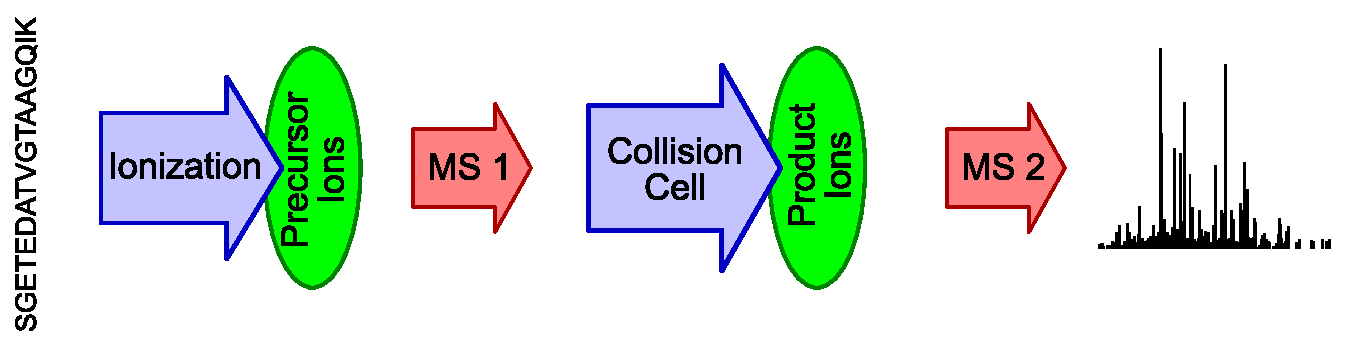
\includegraphics[width=0.9\textwidth]{./img/msms/msms-scheme.eps}
\caption{\label{fig:msms-scheme}
MS/MS scheme. The protein, once purified and digested by Trypsin, undergoes
ionization through MALDI or ESI, the resulting precursor ions are separated
in the first analyser MS$_1$. A selected precursor ions is fragmented in the CID
(see text) and the resulting product ions are separated by the second analyser
MS$_2$ to be recollected in the experimental spectrum on the basis of their
mass-to-charge ratio.}
\end{figure}


So far, the peptides, produced from the enzymatic digestion of an ensemble of
identical proteins, have been separated according to their mass/charge ratio in
the first MS analyser. The determination of their masses can be sufficient for
the identification of the protein by peptide fingerprinting, as described in the
previous chapter, provided that a protein database containing its sequence is
available, and the identification is not hindered by post-translational
modifications that change the mass of the ``bare'' peptide. However, to proceed
further towards a true sequencing of each peptide, a mechanism is needed to
resolve the individual amino-acid residues that compose the peptide. To this
end, Collision Induced Dissociation is combined to a second MS analyser,
according to the following protocol (see Fig.~\ref{fig:msms-scheme} for a scheme
of the process)..

The molecular ions that travel from the first analyser are
accelerated by some electrical potential to high kinetic energy in the vacuum of
the mass spectrometer and then allowed to collide with neutral gas molecules
(often helium, nitrogen or argon). In the collision some of the kinetic energy
is converted into internal energy which results in bond breakage and the
fragmentation of the molecular ion into smaller fragments. 
whose number depends on the energy involved in the collision. Typically,
low-energy CID (the one that we will deal with in more detail) split the
``parent peptide'' in two fragments, a N-terminal and a C-terminal one, while
high-energy CID can yield internal fragments, braking the parent peptide in more
than one point.

While CID is currently the most popular method for standard tandem
mass spectrometry, there are other also other fragmentation methods for special
purposes, for example electron-transfer dissociation (ETD), electron-capture
dissociation (ECD), and infra-red multi-photon dissociation (IRMPD). Alternative
fragmentation methods are particularly useful for identification of
phosphorylation sites and other post-translational modifications
(PTMs).
% (see page~\pageref{ptms}).

Peptides fragment in a reasonably well-documented manner
\cite{roepstorff1984nomenclature,johnson1989interpretation} even if the
underlying physics is not completely understood, and it is not feasible, at the
moment, to predict the outcoming distribution of charged and neutral fragments,
since they depend not only on the composition but also on the conformational
state of the peptide during the
collision\cite{dancik1999,gygi2004nature,Wan2006,Zhang2004}. 
Fragmentation generally occurs between two consecutive residues, breaking a
peptide bond on the main chain of the peptide, this can happen in three different ways generating three
corresponding pairs of fragments (see Fig.~\ref{fig:frag}).
The first fragmentation site is localised on the bond between the $C_\alpha$ carbon
and the subsequent $C=O$ of the same residue while the proton carrying the
positive charge could be alternatively associated to the N-terminal fragment,
giving rise to an $a$ type ion, or to the C-terminal fragment, giving rise to a
$x$ type ion.
The second fragmentation site is between the C-terminal of the carboxyl group of a
residue and the amino group of the following residue, giving rise to the $b$
and $y$ type ions for the N and C-terminal parts respectively.
Last fragmentation site can be found between the amino group and the $C_\alpha$
carbon of the same residue, giving rise to $c$ and $z$ ions.
\cite{roepstorff1984nomenclature,Johnson1987}
Only the fragments carrying the charge inherited from the precursor ion produce
an event on the resulting spectrum.
While the resulting distribution of ions is not predictable, ions labelled $b$
and $y$ are the most observed.

\begin{figure}
\centering
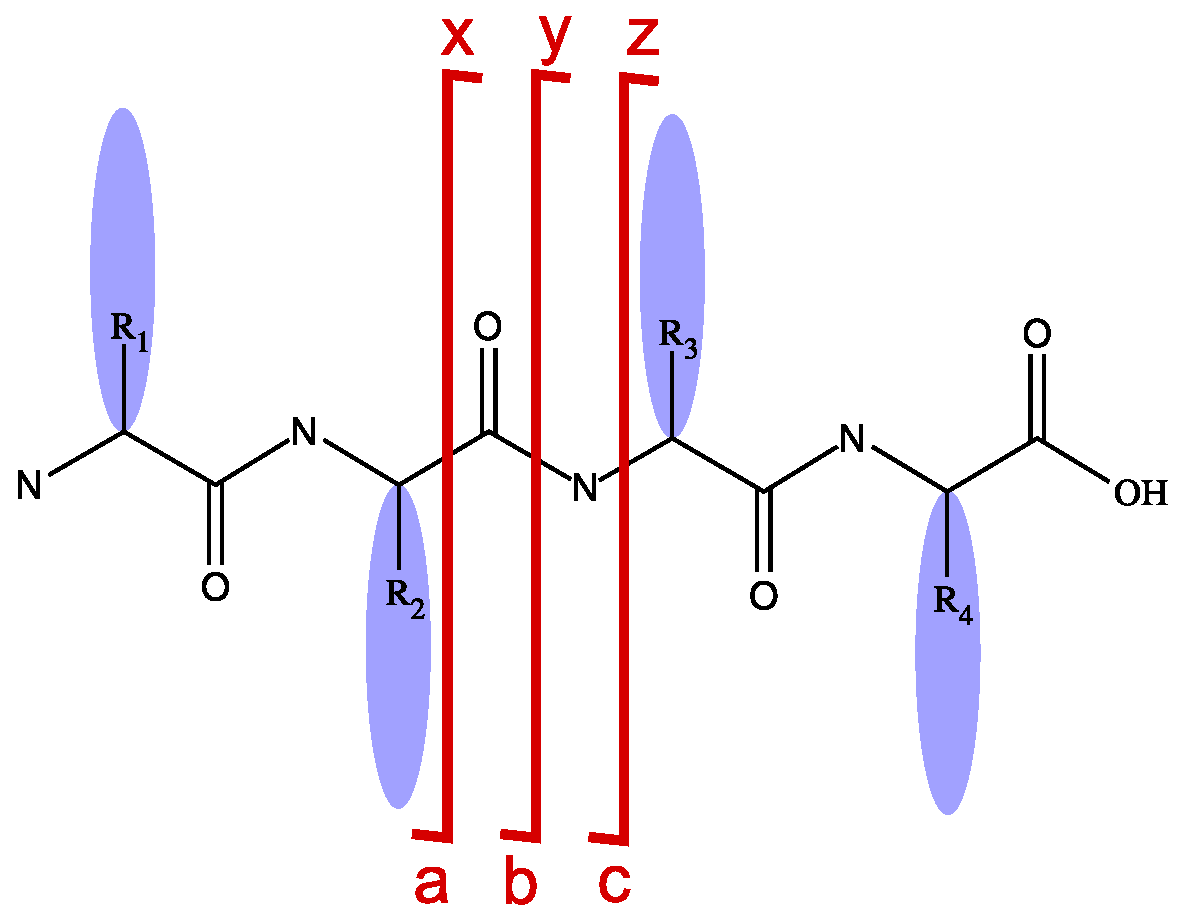
\includegraphics[width=7cm]{./img/msms/amino-cleavage.eps}
\caption{\label{fig:frag}Peptide fragmentation scheme. Ions families
produced by the CID fragmentation of the precursor ions, distinguished by
fragmentation pattern.
Fragments $a,b$ and $c$ are the N-term part of the fragmentation in the NH-CH,
CH-CO, and CO-NH bonds respectively, while $x,y$ and $z$ correspond to the
C-terminal part of the same fragmentations. }
\end{figure}


To make things more difficult, during collisions the fragment ions can undergo
neutral losses (loosing, for instance, water or ammonia groups) or accept more charges
depending on the precursor charge state depending on the residues composing the
resulting ion.
If the precursor ion is carrying more than one charge, the outcoming singly
charged ions can accept a further proton increasing its charge state if the ion
contain at least a Lysine (K), an Arginine (R) or a Histidine (H), this results
in a observed peak at half the joint mass of the product ion and the proton.
Some residues, during the collision dissociation can loose a neutral group,
the most common neutral groups are water (lost by Serine (S) and Threonine (T))
that results in a second peak shifted by -18.01 Da. from the original peak,
ammonia (Glutamine (G), K, R) with a peak shift of -17.03 Da., and urea (R) with
a peak shift of -97.98; while H and R can accept a water group resulting in a
new peak shifted by +18.01 Da..

Another difficulty source for a straight spectrum interpretation is the presence
in the observed ions of elements with high isotopes content, such as carbon and
nitrogen, the highest peaks are then often accompanied by isotopes peaks shifted
by 1 Da. that become important for bigger ion masses. It is feasible that more
than one isotope peak is found if heavier ions are presents.

%\subsection{interpretation}
The resulting charged fragments are detected by the second MS analyser, and add
up to the parent peptide spectrum.
If  fragmentations at every position along the sequence were equally likely, and
if no noise from impurities or contaminants were present, the resulting spectrum
would consist of a series of N-series and C-series peaks, of equal intensity, as
in Fig.~\ref{fig:spectrum-teo}.
The determination of the sequence would be possible by simply reading out the
masses of the component residues from the difference in the position of the
peaks along the $m/z axis$. However, things are more complicated than that, and
a typical spectra looks like the one in Fig.~\ref{fig:spectrum-exp}, 
where true peaks are mixed with noise peaks, of similar
intensity, or can be missing from the spectrum, complicating the task of a
correct identification of the underlying parent peptide sequence.
Moreover, a typical spectroscopy experiment may produce several hundreds of thousands of
precursor spectra that have to be interpreted separately, which calls for an
automated  interpretation resorting to computer programs.

\begin{figure}
\centering
\subfigure[]{
\includegraphics[angle=-90,width=0.45\textwidth]{./img/msms/spec-theo-aby.eps}
\label{fig:spectrum-teo}}
\subfigure[]{
\includegraphics[angle=-90,width=0.45\textwidth]{./img/msms/spec-exper.eps}
\label{fig:spectrum-exp}}
\caption{\label{fig:spectrum}Comparison of the expected theoretical spectrum
(left) including only the most observed fragment,
$y$ ions (red), $b$ ions (green) ans $a$ ions (blue), with the
experimental spectrum (right) for the peptide VINQLTGGLAGMAK.}
\end{figure}

The final outcoming spectrum is a list of paired values of mass-to-charge
ratios and peak intensities where, the first value represent the mass centroid of the observed peak
while the second correspond to the peak area or intensity, that is the total
number of observed events.
Notice that the discrete nature of the resulting peaks
is, actually, a product of the automatic post-processing implemented by the
analyser software: both for the parent peptide and for the fragments, the raw
signal is a continuous one, with  a noise background characterized by small
fluctuations around a mean intensity, which add to high peaks, more or less
intense or well resolved. Not all the peaks can be considered as representing
the true signal: they could also come from an extremal noise fluctuation, or
from common contaminants of several kinds. 
The raw signal is processed to
eliminate everything  below an arbitrarily chosen value (considered as
background noise), and to report in the output file, for each peak, its position
(as the peak or the centroid position) and intensity (as the peak height, or
sometimes the peak area).




The files provided by the SEQUEST algorithm (*.dta) from Finnigan LCQ data
represent one of the most common file format and contain this information.
The first line of the file presents the mass of the single charged precursor ion
$m(MH^+)$ and its actual charge state $Q$.
From the second line until the end, the file include the list of peaks
$(\rho_\alpha,I_\alpha)$. 


%...FIN QUI.  MAGARI SI POTREBBE AGGIUNGERE QUALCOSA SULLE PRECISIONI SULLE INTENSITA' (A SECONDA DELLE DIFFERENTI TECNICHE UTILIZZATE.)

%%%%%%%%%%%%%%%%%%%%%%%%%%%%%%%%%%%%%%%%%%%%%%%%%%%%%%%%%%%%
\section{Protein Sequencing}
%%%%%%%%%%%%%%%%%%%%%%%%%%%%%%%%%%%%%%%%%%%%%%%%%%%%%%%%%%%%

Protein sequencing experiments produce an huge amount of MS/MS spectra,
and the latter are interpreted in order to infer the precursors composition and
sequence.
The spectrum interpretation in the ideal case should be solved by simple
differences of the $m/z$ ratio of the spectrum ideal peaks, and the conversion
of those values in a sequence of amino-acids.
This ideal situation is far from the real case which is affected by instrument
noise and other complexities intrinsic to the system like the presence of
different isotopes in each ions that results
in multiple peaks or the internal fragmentations and neutral losses in product ions,
as discussed in the previous section.
Thus, in the real case spectrum interpretation 
%This process 
is managed by essentially two types of computer algorithms:
\emph{data-base} search and \emph{de-novo} search.
The former is the most popular and actually the most effective and fastest,
provided that some conditions are fulfilled. It
consists in searching the precursor spectrum against a data-base containing well known
sequences.
\emph{De-novo} identification relies only on the information enclosed in the spectrum to
infer its amino-acid sequence.


%%%%%%%%%%%%%%%%%%%%%%%%%%%%%%%%%%%%%%%%%%%%%%%%%%%%%%%%%%%%
\subsection{Database Sequencing Algorithms}
%%%%%%%%%%%%%%%%%%%%%%%%%%%%%%%%%%%%%%%%%%%%%%%%%%%%%%%%%%%%

With the increase of popularity of Tandem Mass Spectral peptide sequencing,
computer automated algorithms for spectra interpretation become available. They
solved the sequencing problem by providing a database of theoretical spectra of
candidate peptides. 

The most popular protein sequencing algorithms are usually shipped with the
spectroscopy instrumentation or maybe purchased separately.
Two commonly used algorithms are Mascot\cite{eng1994} and
SEQUEST\cite{Perkins1999}, which are closed-source software.
They typically correlate the theoretical peptide sequence to the unknown mass
spectrum and match them with a correlation or cost function.

SEQUEST, as an example, provide a huge database of known sequenced proteins.
After filtering the entire database on the bases of the precursor mass and
digestion rules, the
program acts in three steps: in the first step, the experimental data are
reduced filtering out all but the 200 highest peaks and normalizing them to an
intensity of 100, in the second step the algorithm 
calculates the masses of the expected $y$ and $b$ ions from the database sequences, building a theoretical
spectrum, and compares them to the filtered target spectrum through an empiric
score function. 
In the last step the 500 best sequences are then compared by cross-correlation to the
experimental fragments, this include the reconstruction of a more accurate theoretical
spectrum incorporating less abundant ions and intensity informations based on
empirical observations. Once filtered out the precursor ion from the target
spectrum and performed a local normalization of the observed ions, a
cross-correlation function (XCorr) is calculated to attribute the final score.
The difference in score between the first- and second-ranked sequence
($\Delta$Cn) is used to distinguish false positives. 

Mascot scoring algorithm calculates the probability that the match between
experimental data and the theoretical spectrum is a chance event, where the sequence
with lower probability is the best candidate. However the details of the model
have not been published.


This kind of approach, based on a database searching algorithm,
 is very effective in standard condition, but is affected by a
number of weaknesses. 
The use of a sequence database, which is finite per definition, translate in a
finite number of possibly sequencing precursors. 
If the proteome of the  cell is absent from the database, the resulting sequence
inferences are likely to be incorrect.
The target peptide can be absent from the database for a number of reasons, for
instance, depending on the purposes of the experiments, the target protein can
be a mutated one or can present a post-translational modification (PTMs).

%%%%%%%%%%%%%%%%%%%%%%%%%%%%%%%%%%%%%%%%%%%%%%%%%%%%%%%%%%%%
\subsection{\emph{de-novo} Sequencing Algorithms}
\label{subsec:others}
%%%%%%%%%%%%%%%%%%%%%%%%%%%%%%%%%%%%%%%%%%%%%%%%%%%%%%%%%%%%


Another approach to the peptide sequencing problem is through a \emph{de-novo} 
algorithm.
This new approach selects an amino-acid sequence over some candidate peptides
according to a given scoring function. Usually a theoretical spectrum is generated from
the peptide, following some known fragmentation rules, and compared to the
experimental one.
The scoring function, on which each algorithm relies, measures the
similarity of those two spectra and finally the best candidate is reported.
The scoring function is then the core of the algorithm and the overall quality
of the predictions depend on the ability of the scientist to describe all the
significant processes the system undergoes.

In this situation the reconstruction of the peptide sequence in not affected by
any database constraint. 
This approach would therefore be very useful in situations where the genome of
the organism is unknown or just partially known, providing an incomplete protein
database, but also in the case of known genomes, when the existence of some
post-translational modifications (PTMs) to specific residues, provokes peak
displacements and a combinatorial number of possible alternative
interpretations, impairing the \emph{database search} approach for sequencing.

Various algorithms have been developed to solve the \emph{de-novo} peptide
sequencing problem. 
They use different approaches, and various scoring function have been written to
select the best precursor peptide sequence.


\paragraph{Lutefisk}
\cite{lutefisk1997,lutefisk2001} creates a weighted graph using  a simple
scoring scheme. 
A small set of pre-filtered ions from the target spectrum are
interpreted alternatively as $b$ and $y$ fragment as it is impossible \emph{a
priori} to distinguish between them. Successively $b$ ions and $b$-type images of
$y$ ions are recollected in a ``sequence graph''.
The resulting sequences are build ``jumping'' from a node to another if
separated by a length equal to a residue mass (or multiple residues masses) and
sequences connecting N- to C-terminal are stored for further analysis.
The sequences set undergoes a series of filters and best ones are selected
accounting for the interpretable fraction of peaks intensity.

\paragraph{PEAKS}
\cite{peaks2003} creates a similar weighted graph and at each node an empirical
cost-function is evaluated in terms of presence-absence of the relatives $y$ and
$b$ ions, increasing their reward if other ions types (like $x,y-NH_3$ and
$y-H_2O$ for the C-terminal or $a,c,b-NH_3$ and $b-H_2O$ for the N-terminal)
can be matched on the spectrum.
A set of the best 10000 sequences are efficiently calculated in PEAKS and in a
following step a similar but more stringent and computationally inefficient
scoring scheme is applied in order
to produce the final output.

\paragraph{Sherenga}
\cite{dancik1999}, starting from the target spectrum, constructs a graph in which
each node corresponds to a N-terminal peptide fragment, having interpreted a
experimental peak as a given ion type (i.e. $b$ type ions).
Nodes are connected if they differ of about the mass of a residue and are
weighted depending on a learned function of the relative intensities
of the peaks produced by the same fragmentation site.
The resulting problem is to find the path with the highest score which is
solved with a fast dynamical programming algorithm.
 
\paragraph{PepNovo}
\cite{pepnovo-analchem-2005} rely on a probabilistic description of the CID
process and generates a network fragmentation model to find the most probable
sequence. 
Similar to the previous model and in some sense an improvement of it, PepNovo
compares at each sequence site $m$ the score of a fragmentation site interpretation,
based on a semi-empirical probabilistic network of fragmentation rules, with
the hypothesis of random events.
A weighted graph of fragmentation sites nodes is then constructed, with links connecting nodes
separated by a residue mass, and through a dynamical programming algorithm the
highest scoring path is found.

\paragraph{NovoHMM}
\cite{fischer2005novohmm} use a Hidden Markov Model to approach the peptide
sequencing problem. The algorithm combine a learned ``transition probability''
between two residues and the ``emission probability'' of the expected spectrum
ions.
These probabilities are then combined in a factorial Hidden Markov Model.
To simplify the model, only $y$ and $b$ ions are modelled and, thanks to the
symmetry of the resulting algorithm, sequence is folded and the whole chain
divided in two sub-chains. The algorithm start generating sequences at both ends
of the chain and the two part are merged when it reach the centre.

However, the \emph{de novo} sequencing problem in tandem mass spectrometry
remain an open problem.
The information included into mass spectrometry is partially ambiguous, 
as it is not possible, for example, to distinguish between Leucine $L$ and Isoleucine
$I$ relying only on peaks information, since the two residues have exactly the
same atomic composition and, hence, mass. 
Moreover, spectra are usually incomplete and noisy:
low values of mass-to-charge are often not observed, while some
fragmentation sites are naturally protected from low energy fragmentation like in CID as in
Proline bond. Ions other than $y$ and $b$ are usually found with low abundance
and often are completely absent from the spectrum.
Noise peaks help misinterpretation, they can depends on sensor noise or on
sample contamination due to the preparation of the sample for the measure.

Nevertheless the development of algorithms for \emph{de novo} sequencing of
product peptides can enhance the biochemical studies expanding the researches
possibilities or improving already existing database searching algorithms.


\subsection{Reliability of the identification}
\label{sec:reliability}
A common problem for both database and \emph{de-novo} approaches  is to assess the
goodness of the interpretation.   A good score, in either database-search of
\emph{de-novo} sequencing, does not necessarily imply that  the identification is
correct.
This important issue is somewhat mitigated, especially for database searching
algorithms, by the fact that the usual goal in proteomics is to identify
proteins, and not individual peptide sequences. In this sense, redundancy can
balance the uncertainty: the identification of a certain number of peptides as
belonging to a certain protein can be considered  as a proof of the correct
identification, even if none of the individual interpretations is reliable
enough. However, this has some important drawback: in this way it is easy to
correctly recognize  common and highly expressed proteins, that in some sense
could be the ``trivial'' ones, while important proteins appearing in low
abundance can go unnoticed, since their identification is based on the correct
characterization of perhaps just one or a few, possibly low quality spectra. 

So, the assessment  of the reliability of peptide  identification is indeed an
important issue, and, unfortunately,  there is no well-founded theoretical
estimate of the significance of the scores, so that  different empirical methods
have been proposed.
For database search, where the sequence space to be searched is much smaller
than for the \emph{de novo} case, the approach to this problems involves the definition
of a few indicators of the quality of the prediction, as for instance, the
p-value of the score, or the gap in the score between the first and second hit
in the sequence database. For instance, MASCOT score is itself related to a
p-value, since it is based on the probability that the top hit is a random
event, and on the size of the sequence database searched
%\cite{in-MASCOT-NON-C-E-,-PERO-L-HO-TROVATO-CITATO-IN-MenschaertVanCriekinge_JProteomeRes_9_2051-61_2010}.
\cite{Menschaert2010}.
Since the scores are not really rooted on a sound modelling of the fragmentation
process and of the noise distribution, the probability distribution of the score
values cannot be derived from first principles, and involve strong
approximations.
Indeed, it is estimated that just 20\% of MS/MS spectra is successfully
identified by database-matching algorithms\cite{Marcotte2007}.


%[LA PARTE QUI SOTTO, ISPIRATA DA kim\_Pevzner\_JProteomeResearch,2008,3354-3363] 
The problem  of the reliability of the identifications  is a very well known
problem, and several methods have been proposed to assess the value of the
predictions, in a post-processing of the sequencing process \cite{Kim2008}. 
The lack of good theoretical estimates for the statistical significance of
peptide identification prompts for the use of empirical database-dependent
estimates of error rates (resorting to Hypergeometric, Gaussian, Poisson, or
other distributions to predict the probability that a fragment ion matches a
peak, and to calculate the probability that a match between a peptide and a
spectrum is random). A ``better'' practice, recommended  by the Proteomics
Publication Guidelines,  is to search  a decoy database, to
%For instance, in SEQUEST the reliability of the score is evaluated by estimating 
estimate the probability that a match to a random peptide has the same value as
the one obtained for the identified parent peptide. Basically, the idea is to
learn the  null-hypothesis distribution of the scores of random matches from a
``decoy'' database of wrong peptides, generated by the inversion of the
sequence, or involving a more general  reshuffling of the residues. Obviously,
the conclusions on the reliability of the score, drawn in this way, strongly
depends on how accurate the decoy database is.

Other approaches aim at giving a global estimate of the quality of the match, by
training a classification algorithm on spectra of known identity 
\cite{proteinprophet2002}, to be able to distinguish correct
and incorrect matches. Again, this approach depends on the choice of the
training database.

As pointed out by Kim and co-workers
\cite{Kim2008}, the need for a decoy database is a
consequence of the inability to solve the Spectrum Matching Problem: Given a
spectrum $S$ and a threshold T for a scoring function, find the probability that a
random peptide matches $S$ with score greater than $T$. This quantity, which
represents the False Positive Rate, is quite difficult to estimate correctly,
and is usually replaced by the False Discovery Rate, which is not a
characteristic of the individual spectrum, but rather an average property, i.e.
the fraction of incorrect guesses among all identifications with score greater
than $T$.



The situation is perhaps even worse for \emph{de novo} interpretation.
Basically, all the score functions to assign a quality to the interpretation are
empirically derived, and tested against a test-bed of spectra, whose
interpretation is considered reliable. Hence, indications of precision and
recall can be given for each method, stating how many times, on average, the
method does a good job in guessing the parent peptide that originated the
spectra (we will make this statements more precise in
Chapter~\ref{chap:msms-results}). 
For each spectrum, a list of best scoring sequences is usually
produced, along with the corresponding score, but there is no real way to
determine how reliable the interpretation is.


%%%%%%%%%%%%%%%%%%%%%%%%%%%%%%%%%%%%%%%%%%%%%%%%%%%%%%%%%%%%
%%%%%%%%%%%%%%%%%%%%%%%%%%%%%%%%%%%%%%%%%%%%%%%%%%%%%%%%%%%%
\chapter{Spectral Interpretation as a Statistical Mechanics Problem}
\label{chap:alg}
\nopagebreak
%%%%%%%%%%%%%%%%%%%%%%%%%%%%%%%%%%%%%%%%%%%%%%%%%%%%%%%%%%%%
%%%%%%%%%%%%%%%%%%%%%%%%%%%%%%%%%%%%%%%%%%%%%%%%%%%%%%%%%%%%

We have seen in the previous chapter the strategy underlying protein sequencing
by MS/MS, the interpretation problems that have to be faced, and the present
methods to deal with them.
We have also seen the pros and cons of the two approaches to MS/MS spectra
interpretation: database-search and \emph{de-novo} sequencing, and have discussed the
issue of the statistical significance of the score of the reported precursor
sequence.

Basically, all sequencing algorithms, both database-searching and \emph{de-novo}, yield
as a result the solution with the highest score (or, equivalently, with the
lowest energy, if we define an energy as the negative score): from this point of
view, the only difference between them is given by the state-space of the
search, which is just the database in the former case, or all the sequence space
of a given mass in the latter.
Therefore, we can say that they find the ground-state, or zero-temperature
solution, in the appropriate sequence space. Suboptimal solutions, as proposed
in the ranked list, corresponding to the excited states, are not included in the
solution, but listed a part.
On the other hand, physical intuition suggests that, given a reasonable energy
function to score the match between a proposed sequence and the experimental
spectrum, poor quality spectra, with a low signal/noise value (defined in some
suitable sense), should correspond to high energy and/or high entropy. Indeed, a
high number of excited states at small gap from the ground state, representing
alternative solutions with essentially the same energy as the best one, should
point at a bad prediction, possibly related to missing peaks, to the presence of
many or intense noise peaks, or both.

These observations suggest that the introduction of an artificial temperature in
the solutions space, and the study of the resulting thermodynamic equilibrium,
could provide some valuable internal indication of the quality of the
interpretation, in a sense analogous to the False Predictive Rate mentioned in
Section~\ref{sec:reliability}.
For instance, despite the fact that, in a finite system, the existence of real
phase transition is precluded, we could expect that, for each spectrum, there is a
low-temperature phase, where one or a few sequences dominate as candidate
solutions, while at high temperature a ``paramagnetic'' phase exists,
corresponding to a mixture of a huge amount of solutions. The temperature of
transition between the two regimes, as signalled, for instance, by a peak in the
heat capacity, could bring, again, important information on the robustness of
the interpretation -- the higher the temperature, the more reliable the
identification.

In order to exploit the benefits of moving out from the zero-temperature
solution, we need first of all a proper way to map the problem of spectra
interpretation on that of finding the thermodynamic equilibrium of a suitable
physical system, and second, an effective way to actually perform calculations.
In the following, we will deal with both issues: first we will introduce a
discrete unidimensional system, whose states encode all possible amino-acid
sequences of appropriate length. Second, we will define the general form of the
energy function of the model in term of just on-site and next-neighbors
interaction, involving some constraints on the  class of scoring function that
can be implemented in the model. We will leave the detailed derivation of a
particular form of the energy function, inspired by Bayesian modelling, for
Chapter~\ref{chap:pot}, moving forward to introduce a transfer-matrix technique that
allows to calculate exactly the partition function of the model, finding its
equilibrium solution. We will finally discuss how the equilibrium results can be
mapped back to  MS spectra interpretation.

%%%%%%%%%%%%%%%%%%%%%%%%%%%%%%%%%%%%%%%%%%%%%%%%%%%%%%%%%%%%%%%%%%%%%%%%%%%%%%%
\section{Encoding the sequence space on a 1D lattice model}
\label{sec:variables}

A peak in the experimental spectrum gives information on the $m/z$ ratio of the
N- or C-terminal ions (if we neglect the possibility of internal fragments)
obtained in the fragmentation process during CID: such information is not
related to detailed sequence of the fragment ions (even if it can be affected by
the presence of some amino-acid, as we will detail below), but just depends on
the mass and charge of the whole fragment.

We can use this fact to avoid the book-keeping of a combinatorial number of
possible sequences, and to define a physical system whose site variables carry
information on the mass and charge, as well as some other overall quantities
that we will need to characterize completely the parent peptide.
  
Despite the fact that the fragment masses are incommensurable, their
discretization in terms of a unit mass $\eta$, roughly equal to an atomic mass
unit, is a reasonable and natural approximation. Therefore, we define a discrete
one-dimensional lattice  of $M+1$ sites, numbered from $0$ to $M$, where $M$ is
the discretized mass of the parent peptide (more precisely, it is the sum of the
masses of the residues that compose it, neglecting the extra groups H and OH at
the N- and C- term, and neglecting the extra proton of the precursor MH$^+$).
The lattice spacing $\eta$ is given by:
\begin{equation}
\eta=
\sum_{a}\frac{m_{a}^m}{m_{a}}f(a)
=1.0005022782 \,\,,
\end{equation}
the weighted mean of the ratio between the  mono-isotopic residue mass
$m^m_{a}$ and the discrete mass $m_{a}$, where the weight $f(a)$ is the
natural abundance of the residue $a$.

Table \ref{tab:residues} lists  all the residues with their mono-isotopic mass and the corresponding 
discretized value. Testing the model, in Chapter~\ref{chap:msms-results}, we will ignore
post-translational modification and will deal just with sequences made up of
natural amino-acids; however, the following discussion holds valid when PTMs are
present, by simply augmenting Table~\ref{tab:residues} with the corresponding modified
residues masses and corresponding properties.

\begin{table}
\centering
\begin{tabular}{ccccccccc}
\hline \hline
$a$ & $m^m_{a}$ & $m_{a}$ & $f(a)$ & $q$ & $l_1$ & $l_2$ & $l_3$ & $l_4$\\
\hline	
G &  57.021 &  57 & 7.49 & 0 & 0 & 0 & 0 & 0 \\
A &  71.037 &  71 & 5.22 & 0 & 0 & 0 & 0 & 0 \\
S &  87.032 &  87 & 4.53 & 0 & 1 & 0 & 0 & 0 \\
P &  97.053 &  97 & 5.22 & 0 & 0 & 0 & 0 & 0 \\
V &  99.068 &  99 & 1.82 & 0 & 0 & 0 & 0 & 0 \\
T & 101.048 & 101 & 6.26 & 0 & 1 & 0 & 0 & 0 \\
C & 103.009 & 103 & 4.11 & 0 & 0 & 0 & 0 & 0 \\
I & 113.084 & 113 & 7.10 & 0 & 0 & 0 & 0 & 0 \\
L & 113.084 & 113 & 2.23 & 0 & 0 & 0 & 0 & 0 \\
N & 114.043 & 114 & 5.45 & 0 & 0 & 0 & 0 & 0 \\
D & 115.027 & 115 & 9.06 & 0 & 0 & 0 & 0 & 0 \\
Q & 128.059 & 128 & 5.82 & 0 & 0 & 1 & 0 & 0 \\
E & 129.043 & 129 & 2.27 & 0 & 0 & 0 & 0 & 0 \\
M & 131.040 & 131 & 3.91 & 0 & 0 & 0 & 0 & 0 \\
H & 137.059 & 137 & 5.12 & 1 & 0 & 0 & 1 & 0 \\
F & 147.068 & 147 & 7.34 & 0 & 0 & 0 & 0 & 0 \\
Y & 163.063 & 163 & 5.96 & 0 & 0 & 0 & 0 & 0 \\
W & 186.079 & 186 & 1.32 & 0 & 0 & 0 & 0 & 0 \\
K & 128.095 & 128 & 3.25 & 1 & 0 & 1 & 0 & 0 \\
R & 156.101 & 156 & 6.48 & 1 & 0 & 1 & 1 & 1 \\
\hline \hline
\end{tabular}
\caption{\label{tab:residues} List of residues with the corresponding
mono-isotopic $m^m_{a}$ and discrete mass $m_{a}$ as a multiple of $\eta$,
along with the residue natural frequency $f(a)$ (in percentage). 
The likeliness of each residue to accept a charge $q$ or to lose a neutral group
(water ($l_1$); ammonia ($l_2$); accepting water $l_3$; urea $l_4$) is reported
on the following columns (0 means not allowed; 1 means allowed).}
\end{table}

Any sequence of total mass $M$ will be identified, in the lattice, by the
terminal points of each residue, that will coincide (thanks to the mass
discretization) with different lattice sites, situated at a distance
corresponding to the residue's mass. For instance, referring to
Figure~\ref{fig:onesequence}, we will have that the first residue, A, of mass $m_A$,
starts in 0 and ends at $\nu_A$, while  the second residue B, of mass $m_B$, ends at
$\nu_{AB}=m_A+m_B$, etc.

\begin{figure}
\centering
\includegraphics[angle=-90,width=0.6\textwidth]{./img/msms/r.eps}
\caption{\label{fig:onesequence}
Behaviour of the variable $r$ describing the state of the system at the
fragmentation
site $\nu$, it takes the value 0 at the beginning of the first residue and
increases of one at each step of $\nu$. When $r$ reaches the value corresponding
to the mass of the first residue $A$, and then of the second, B, and so on, 
it is constrained back to the value 0.}
\end{figure}

We map the possible amino-acid sequences to model configurations by introducing,
for each site, a variable $r \in [0,r_{max}]$, where $ r_{max}$ is the biggest
residue mass (if post-translational modifications are included, it will
correspond to the heaviest species, be it a wild-type or a modified residue). We
will implement the following rule (by means of a suitable constraint in the
energy function): the only values allowed at $\nu$ are  $r_{\nu}=r_{\nu-1}+1$ or
$r_{\nu} = 0$, the latter just holding when $r_{\nu-1}=m(a)-1$, for some
amino-acid $a$ (natural or modified) from the list of chemical species allowed as
component of the parent peptide. It is easy to convince oneself that the above
rule, together with the boundary conditions  $r_0=r_M=0$, can generate each and
every possible sequence of total mass $M$, identifying the sites $\nu$ where
$r_{\nu}=0$ as those where a residue ends, see Fig.~\ref{fig:onesequence}.
Notice also that the above constraint involves the values of $r$ at neighbouring
sites $r_{\nu}$, $r_{\nu-1}$, and can be dealt with simply as a next-neighbour
interaction.
Given one possible configuration of the system, the sites $\nu$ where
$r_{\nu}=0$ represent possible fragmentation sites of the corresponding parent
peptide. To match them against the spectrum peaks, we need to calculate the
position $m/z$ of the various ions that can be generated during fragmentation,
so that another information that we shall add at each site is the maximal charge
that can carry a N-terminal ion ($q^N_\nu$) or a C-terminal one ($q^C_\nu$),
according to the parent peptide's charge and the number of residues in the
outcoming N- and C-terminal fragments that can loose an electron (K,R,H). The
constraints on the charge are a little more complicated than those  for the mass
variable $r_{\nu}$ (see Appendix~\ref{chap:app_constraints}), but again can be
written in terms of the variables at sites $(\nu-1)$ and $\nu$.

The possible fragments generated in a dissociation at a certain position $\nu$
also depend on the number of residues that can present neutral losses (such as
loss of water, ammonia, phosphate groups, etc.), resulting in a different mass
of the corresponding peak. To carry this information, we introduce two vectors
of integers  ${\bm l}^X_\nu=\{l^X_{\nu,1},\dots,l^X_{\nu,N_l}\}$,
($X=\{N,C\}$),  at each site $\nu$, specifying the  maximal number of neutral
losses of each kind ${\bm l}^N_{\nu,\alpha}$ that can be seen in $X$-terminal
fragments. Here ${\cal L}$ is the number of neutral losses type considered.
The constraints between the values of these vectors at neighbouring site are
similar to those for the charge (see Appendix~\ref{chap:app_constraints}), with
the difference that the maximal number of loss-prone residues in the parent peptide
is not known a priori (while the total charge of the precursor peptide is
measured by the first Mass Spectrometer, and hence known before the
fragmentation process).
In the following chapter, we will limit the number of neutral losses considered
to two, water and ammonia, for reasons that will be discussed there.

Another important information to carry at each site is one related to the nature
of the residue preceding the last one in the peptide sequence: according to the
trypsin cleavage rules, a protein chain will not be cut after Lysine (K) or
Arginine (R) if the following residue is a Proline (P), or if it is another K or
R. 
So, a $\pi_\nu=1$ flag will signal that $\nu$ lies ``inside'' a K, R or P
residue, so that we must remember this constraint at the closer position
$\nu_0>\nu$ where we will terminate the ``current'' residue, putting
$r_{\nu_0}=0$. Without this binary flag, sequences containing K and R at
arbitrary positions would be considered in the configuration space, enlarging
the allowed state space. Actually, this constraint can be softer than the rest,
since it is known that sometimes trypsin fails resulting in one (or at most, a
few) missing cleavage sites, signalled by some isolated K or R.
The above rules are specific to trypsin, which is the most commonly used enzyme
in digestion; if a different enzyme is used, different rules should be
implemented accordingly.
 
The last variable that can be used is the number $n_{\nu}$ of residues
accumulated in the N-terminal part of the chain with respect to the position
$\nu$: this is useful if we want to couple \emph{de-novo} sequencing with database
search, or if we are interested in questions as the probability of finding a
certain amino-acid as the k-th residue of the parent peptide sequence.

At each $\nu$ a fragmentation event can occur and a set of ions can thus be
produced; this
set, which generally is a small subset of the expected ions, will be matched to
the experimental peaks of the target spectrum.
An accurate prediction of the fragmentation pattern is not possible, as discussed
before, and thus we introduce a binary fragmentation variable
$\xi_\nu^{s_i}=0,1$ that account for the event of ion formation, taking the
value 0 if the corresponding ion species $s_i$ is not produced in the CID,
taking the value 1 otherwise.

We collect all the state-variables, characterized above, in a global one,   
$\sigma_\nu\equiv\{r_\nu,q^N_\nu,q^C_\nu,{\bm l}^N_\nu,{\bm
l}^C_\nu,\pi_\nu,n_\nu,\bm \xi_\nu\}$, that will contain all the relevant information needed
at site $\nu$ to yield the correct fragmentation.
As detailed in the Appendix~\ref{chap:app_constraints}, the constraints imposed
on the variables can be resumed in the fact that, if
$r_\nu>0$, $\sigma_\nu$ retains the same values of the state variables  at
position $(\nu-1)$ (except $r_\nu=r_{\nu-1}+1$): the system \emph{remembers} the
state it had at the previous site.
  If $r_\nu=0$, a new residue is ``started'' at $\nu$, and the state variables
on charges, neutral losses, etc. are updated according to the identity of the
residue terminating at $\nu$ (that can be recognized by its mass ($r_{\nu-1}+1$)
and/or state-numbers, with the exception of the couple Isoleucine-Leucine (I-L), see
Table~\ref{tab:residues}).

The set of all $\sigma_\nu$, together with their constraints, describe all the
possible parent peptides, and specify the relevant information to produce the
corresponding  fragmentation and ionization patterns.
To select which peptide sequence and fragmentation pattern best fits the
experimental spectrum, we need an appropriate Hamiltonian, to play the role of
the scoring function.

%%%%%%%%%%%%%%%%%%%%%%%%%%%%%%%%%%%%%%%%%%%%%%%%%%%%%%%%%%%%
\section{The Hamiltonian}
\label{sec:hamiltonian}

We will derive and detail an empirical form of the energy function in
Chapter~\ref{chap:pot}; here we discuss the general form that such function must have,
according to our goals of calculating exactly the corresponding partition
function.


The Hamiltonian will consist of two different parts: 
a first part $H^1$ represents the energy cost of fragmenting in $\nu$ (setting
$r_\nu=0$), 
and depends only on the experimental spectrum $\Sigma$ and fragmentation pattern
at site $\nu$: which and how many ions of the different species, together with
their neutral losses, are generated and match some peaks. This is a completely
local term, acting like an  ``external field'' rewarding or penalizing
fragmentation at $\nu$.
Due to the local nature, it rules out the possibility of describing non-local
events, such as correlations between ion types produced at fragmentations at
neighbouring residues,  correlations between intensities of fragments from
different sites, or the possibility that a peak is actually produced by two
different fragmentations, at different sites, that happen to produce ions with
the same $m/z$ ratio.
  
The second part $H^2$ represents all the constraints, previously mentioned and
described in Appendix~\ref{chap:app_constraints}, related to the internal
consistency of the description of the parent peptide.

$H^1$ and $H^2$ can be written as:
\begin{align}
H^1 &= \sum_{\nu=1}^M H_\nu^1(\sigma_\nu,\Sigma)\\
H^2 &= \sum_{\nu=1}^{M-1}
H_{\nu,\nu+1}^2(\sigma_{\nu-1},\sigma_\nu)
\end{align}

The spectrum part of the Hamiltonian $H^1_\nu(\sigma_\nu,\Sigma)$ is the
sum of the contributions of the expected fragment ions $s_i$: 
\begin{equation}
H^1_\nu(\sigma_\nu,\Sigma)=
%\sum_{s_i} \xi_\nu^{s_i} H_\nu^{s_i}
\sum_{s_i} H(\nu,s_i,\xi_\nu^{s_i})
\label{eq:h1}
\end{equation}

Here $H(\nu,s_i,\xi_\nu^{s_i})$ is the energy of matching the theoretical peak
of type $s_i$, generated at the fragmentation site $\nu$, in the target spectrum and is
of the form $H(\nu,s_i,\xi_\nu^{s_i})=\mu+\delta_{\xi_\mu^{s_i},1}H_\nu^{s_i}$,
where $\mu$ is a model parameter representing a chemical potential (see
Sec.~\ref{potential} for an accurate characterization of this term).

The interaction part of the energy $H^2_{\nu-1,\nu}(\sigma_{\nu-1},\sigma_\nu)$
can take two possible values: zero if the corresponding condition is satisfied, and infinity
otherwise:
\begin{equation}
H^2_{\nu-1,\nu}
\left\{
\begin{aligned}
&0 && 
\left\{
\begin{aligned}
&r_\nu\ne0\\
&r_\nu=r_{\nu-1}+1\\
&q^X_\nu=q^X_{\nu-1}\\
&{\bm l}^X_\nu={\bm l}^X_{\nu-1}\\
&n_\nu=n_{\nu-1}\\
&\pi_\nu=\pi_{\nu-1}
\end{aligned}
\right.\qquad\forall X=\{N,C\}\\
&0 && 
\left\{
\begin{aligned}
&r_\nu=0\\
&r_{\nu-1}=m_{a}-1\\
&q^X_\nu=q^X_{\nu-1}+\delta_q^X(a)\\
&{\bm l}^X_\nu={\bm l}^X_{\nu-1}+{\bm\delta}_l^X(a)\\
&n_\nu=n_{\nu-1}+1\\
&\pi_\nu=\pi_{\nu-1}+\delta_\pi(a)
\end{aligned}
\right.\qquad\forall X=\{N,C\}\\
&\infty && \text{otherwise}
\end{aligned}
\right.
\label{eq:h2}
\end{equation}
where $\delta_q^X(a),\bm \delta_l^X(a)$ and $\delta_\pi(a)$ take the values -1,0,1
and represent the
constraints applied to the first-neighbours interactions.
Fragmentation sites are characterized by $r_\nu=0$ and, in those cases, the
values of contiguous variables in $\nu-1$ and $\nu$ have to fulfil 
the constraints represented by $\delta_q^X(a),\bm \delta_l^X(a)$ and $\delta_\pi(a)$.
The latter depend on the amino acid $a$ ending in $\nu$ and on the
state of the dynamic variables in $\nu-1$ and $\nu$, as described
in the Appendix~\ref{chap:app_constraints}.


%%%%%%%%%%%%%%%%%%%%%%%%%%%%%%%%%%%%%%%%%%%%%%%%%%%
\section{Thermodynamics of the model}

Using the previous definition of the dynamical variable $\sigma_\nu$, a state of
the unidimensional system is defined as
$\phi=\{\sigma_\nu,\nu=1,\dots,M\}$.
The probability of the system to visit the state $\phi$ takes the following form:
\begin{equation}
p(\phi|\Sigma,T)=
\frac{e^{-\beta H(\phi,\Sigma)}}
{\sum_{\phi'} e^{-\beta H(\phi',\Sigma)}}
\label{pot}
\end{equation}
where $H(\phi,\Sigma)$ is the empirical energy function that we use to score the
sequences.
The quantity at the denominator is the partition function, and is the
fundamental quantity to be calculated in equilibrium thermodynamics, since all
the others (free-energy, average energy, entropy, etc.) can be related to it.
Unfortunately, its evaluation involves the sum over all possible states that the
system can assume, which are even more than the possible sequences; considering
that for a little peptide of
only 800 Da there are 70.440.173
different sequences satisfying the
precursor mass constraint, it is easy to understand that a brute-force
calculation is unfeasible.
We will see in the following section how the calculation can be performed in an
efficient way.


Once defined the Hamiltonian one can, in principle, compute interesting
values in the form of statistical expected values:
\begin{align}
U=\langle H \rangle 
&= 
-\frac{\partial}{\partial\beta} \ln Z =
\sum_\phi H(\phi,\Sigma)e^{-\beta H (\phi,\Sigma)}\\
S 
&= 
\beta \left(\langle H\rangle-F \right) =
-\sum_\phi p(\phi)\ln p(\phi)\\
C_V 
&= 
\frac 1 {T^2} \left(\langle H^2\rangle-\langle H\rangle^2\right) \equiv
\frac{\partial \langle H\rangle}{\partial T} = T \frac{\partial S}{\partial T}
\end{align}


Finally, we can derive the probability of a sequence $\widetilde P$ through the
calculation of the marginals:
\begin{equation}
p_\nu(a)=\langle
\delta_{r_\nu,0}\ \delta_{r_{\nu-1},m(a)-1} %\ \delta_{?n_{\nu-1},i}
\rangle
\end{equation}
which represents the probability of the residue species $a$ to end in $\nu$
($r_\nu=0$), while at $\nu-1$ the $r$ counter has reached a value corresponding
to the discretized mass of the residue $a$.

We will come back to the explicit calculation of above quantities in the
following sections.


\subsection{The Transfer-Matrix Method}
With the definition of $H^1$ and $H^2$, the system presents only first-neighbour
interactions as only $H^2$ presents a correlation between adjacent subsystems in
$\nu-1$ and $\nu$.
In this situation it is possible to resort to the transfer-matrix method,
in which the partition function $\mathcal{Z}$ can be calculated incrementally.
We write  $\mathcal{Z}$  as:
\begin{align}
\mathcal{Z} =& \sum_{\substack{\{\sigma_\nu\}\\\nu=1\dots M}}
\exp(-\beta \sum_{\nu=1}^M H^1(\sigma_\nu) -\beta \sum_{\nu=1}^M
H^2(\sigma_{\nu-1},\sigma_\nu)))\\
=&
\sum_{\lbrace\sigma_\nu\rbrace} 
%e^{-\beta H^1_1} 
\prod_{\nu=1}^M
{ e^{-\beta H_{\nu-1,\nu}(\sigma_{\nu-1},\sigma_\nu)}
}
\label{eq:z}
\end{align}
where $H_{\nu-1,\nu}(\sigma_{\nu-1},\sigma_\nu)=
H^1_\nu(\sigma_\nu)+H^2_{\nu-1,\nu}(\sigma_{\nu-1},\sigma_\nu)$, and the first
term on the N-terminal edge is taken as $H^1(\sigma_0)=0$.

We introduce, then, the reduced partition function $\mathcal Z_\mu$ that refer to the
partition function of the
subsystem limited to values of $\nu$ in $[0,\mu]$ as in the following:
\begin{align}
\mathcal Z_\mu &=
\sum_{\substack{\{\sigma_\nu\}\\\nu=1\dots\mu}} e^{-\beta H}
=
\sum_{\substack{\{\sigma_\nu\}\\\nu=1\dots\mu}} \prod_{\nu=1}^{\mu} e^{-\beta
H_{\nu-1,\nu}
(\sigma_{\nu-1},\sigma_\nu)}
\\&=
\sum_{\sigma_\mu}W_\mu(\sigma_\mu)
\end{align}
where we have introduced the vector $W_\mu(\sigma_\mu)$ defined as: 
\begin{equation}
W_\mu (\sigma_\mu)=
\sum_{\substack{\{\sigma_\nu\}\\\nu=1\dots\mu-1}}
\prod_{\nu=1}^\mu
e^{-\beta H_{\nu-1,\nu}(\sigma_{\nu-1},\sigma_\nu)}
\end{equation}

We can actually write the vector $W_\mu(\sigma_\mu)$ as a function of the previous
values at $\mu-1$, $W_{\mu-1}(\sigma_{\mu-1})$:
\begin{align}
W_\mu(\sigma_\mu)
&=
\sum_{\sigma_{\mu-1}}
\left(
\sum_{\substack{\{\sigma_\nu\}\\\nu=1\dots\mu-2}} \prod_{\nu=1}^{\mu-1}
e^{-\beta H_{\nu-1,\nu}(\sigma_{\nu-1},\sigma_\nu)}\right)
e^{-\beta H_{\mu-1,\mu}(\sigma_{\mu-1},\sigma_\mu)}
\nonumber\\
&=
\sum_{\sigma_{\mu-1}}
W_{\mu-1}(\sigma_{\mu-1})
e^{-\beta H_{\mu-1,\mu}(\sigma_{\mu-1},\sigma_\mu)}
\end{align}

The above expression can be seen as a vector equation, if we introduce a state
vector at site$\nu$, $\mathbf{W}_\nu$, whose components are labelled by the
possible states of the variable $\sigma_\nu$, and a Transfer Matrix
$\mathbf{T}_{\nu,\nu-1}$ between sites $(\nu-1)$ and  $\nu$, of elements
$(T_{\nu,\nu-1})_{\sigma_\nu,\sigma_{\nu-1}}$, that carries the information
between neighbouring sites; namely.
\begin{equation*}
 \mathbf{W}_\nu={\mathbf T}_{\nu,\nu-1} \mathbf{W}_{\nu-1}\,\,,
\end{equation*}
which justifies the name of ``transfer matrix method'' of this section.

 
Due to the exponential function, at low temperature the above quantities can
become very large, so that to avoid computation problems in the implementation
of the algorithm as a computer code,
we can introduce the normalized %recursively computable
$\zeta_\mu(\sigma_\mu)$ as:
\begin{equation}
\zeta_\mu(\sigma_\mu)=
\frac1{Z_\mu}W_\mu(\sigma_\mu)=\frac{Z_{\mu-1}}{Z_\mu}\sum_{\sigma_{\mu-1}}
\zeta_{\mu-1}(\sigma_{\mu-1}) e^{-\beta H_{\mu-1,\mu}}
\label{zeta_mu}
\end{equation}

We define, then, $\phi_{\mu-1,\mu}$ as the ratio between the reduced partition function
of the $\mu$ subsystem and the reduced partition function of the $\mu-1$
subsystem.
Given the following relations:
\begin{align}
Z_\mu &=
%\sum_{\sigma_\mu} \sum_{\sigma_{\mu-1}} \left[
\sum_{\sigma_\mu,\sigma_{\mu-1}} \left[
W_{\mu-1}(\sigma_{\mu-1}) \left( e^{-\beta
H_{\mu-1,\mu}}-\delta_{\sigma_\mu,\sigma_{\mu-1}}\right)+
\delta_{\sigma_\mu,\sigma_{\mu-1}} W_{\mu-1}(\sigma_{\mu-1}) \right]\nonumber\\
&=
%\sum_{\sigma_\mu} \sum_{\sigma_{\mu-1}}
\sum_{\sigma_\mu,\sigma_{\mu-1}}
W_{\mu-1}(\sigma_{\mu-1}) \left(
e^{-\beta H_{\mu-1,\mu}}-\delta_{\sigma_\mu,\sigma_{\mu-1}}\right)+
Z_{\mu-1}\nonumber\\
&= 
Z_{\mu-1} \left[ 1+\sum_{\sigma_{\mu-1}}
\frac{W_{\mu-1}(\sigma_{\mu-1})}{Z_{\mu-1}} \left(\left(
\sum_{\sigma_\mu}e^{-\beta H_{\mu-1,\mu}}\right)
-1\right)\right]
\label{z_mu}
\end{align}
one can write:
\begin{equation}
\phi_{\mu-1,\mu}=
\frac{Z_\mu}{Z_{\mu-1}}=
1+\sum_{\sigma_{\mu-1}}
%\frac{W_{\mu-1}(\sigma_{\mu-1})}{Z_{\mu-1}} 
\zeta_{\mu-1}(\sigma_{\mu-1})
\left(\left(
\sum_{\sigma_\mu}e^{-\beta H_{\mu-1,\mu}}\right)
-1\right)
\end{equation}



Following the same method used to calculate the value of the partition function
we can calculate the value of other important thermodynamics quantities.

\subsection{Average Energy}

Starting from the definition of  $\langle\beta E\rangle = \mathcal{Z}^{-1}
\sum_{\sigma_\nu} H \exp(-\beta H)$ that we can rewrite as:
\begin{equation}
\langle \beta E \rangle=
\frac{1}{Z}
\sum_{\substack{\{\sigma_\nu\}\\\nu=1\dots M}} \left(
\sum_{\alpha=1}^M\beta H_{\alpha-1,\alpha}(\sigma_{\alpha-1},\sigma_\alpha)
\right)
\prod_{\nu=1}^M e^{-\beta H_{\nu-1,\nu}(\sigma_{\nu-1},\sigma_\nu)} 
\end{equation}
we notice that we can introduce the mean energy $\langle\beta E_\mu\rangle$ for the subsystem
$\nu=0\dots\mu$ as:
\begin{equation}
\langle \beta E_\mu \rangle =
\sum_{\sigma_\mu} 
\varepsilon_\mu(\sigma_\mu)
\end{equation}
where, as in the case of $\zeta_\mu(\sigma_\mu)$, we have that:
\begin{equation}
\varepsilon_\mu(\sigma_\mu)=
\frac 1{Z_\mu}
\sum_{\substack{\{\sigma_\nu\}\\\nu=1\dots\mu-1}}
\left(
\sum_{\alpha=1}^{\mu} \beta H_{\alpha-1,\alpha}(\sigma_{\alpha-1},\sigma_\alpha)
\right)
\prod_{\nu=1}^{\mu}
e^{-\beta H_{\nu-1,\nu}(\sigma_{\nu-1},\sigma_\nu)}
\end{equation}
and with a little of maths we can write $\varepsilon_\mu(\sigma_\mu)$ as a
function of its predecessor $\varepsilon_{\mu-1}(\sigma_{\mu-1})$


\begin{multline}
\varepsilon_\mu(\sigma_\mu)= 
\frac {Z_{\mu-1}}{Z_\mu} \sum_{\sigma_{\mu-1}} \Big[
\varepsilon_{\mu-1}(\sigma_{\mu-1})+\\
+\beta H_{\mu-1,\mu}(\sigma_{\mu-1},\sigma_\mu)\zeta_{\mu-1}(\sigma_{\mu-1})
\Big]e^{-\beta H_{\mu-1,\mu}}
\label{epsilon_mu}
\end{multline}

The final value of $\langle\beta E\rangle$, can then be calculated from the
value of $\varepsilon_M(\sigma_M)$ in the following way:
\begin{equation}
\langle \beta E\rangle =
\langle \beta E_{\mu=M} \rangle
=
\sum_{\sigma_M} \varepsilon_M(\sigma_M)
\label{mean_b_e}
\end{equation}



\subsection{Heat Capacity}

%In the following we compute the Specific Heat $C_V$ for the system at a given
%temperature $T$.
%Its behaviour can tell us if the system is on a
%``energetic regime'', where it visits only low energy
%states, or in a ``entropic regime'', where the fluctuations of the system are
%large and the latter can visit many high energy states.

To calculate the heat capacity $C_V=\langle\beta^2E^2\rangle-
\langle\beta E\rangle^2$, we have to calculate the mean of the square energy:
\begin{equation}
\langle \beta^2 E^2 \rangle =
\langle \beta^2 E^2_{\mu=M} \rangle_{(1\dots M)}\nonumber
\end{equation}

We introduce the $\mu$-subsystem mean square energy
$\langle\beta^2E^2_\mu\rangle$ and $c_\mu(\sigma_\mu)$ as before:
\begin{align}
\langle \beta^2 E^2_\mu \rangle &=
\frac 1 {Z_\mu}
\sum_{\substack{\{\sigma_\nu\}\\\nu=1\dots\mu}}
\left(\sum_{\alpha=1}^\mu \beta
H_{\alpha-1,\alpha}(\sigma_{\alpha-1},\sigma_\alpha) \right)^2 \cdot
\prod_{\nu=1}^\mu e^{-\beta
H_{\nu-1,\nu}(\sigma_{\nu-1},\sigma_\nu)}\nonumber\\
&=
\sum_{\sigma_\mu} c_\mu(\sigma_\mu)
\end{align}
%using:
%\begin{eqnarray}
%\left(\sum_{\alpha=1}^\mu \beta H_{\alpha-1,\alpha}\right)^2 &=&
%\left[\left(\sum_{\alpha=1}^{\mu-1}\beta H_{\alpha-1,\alpha}\right)^2+
%\right.\nonumber\\
%&\ & \left.+
%2\left(\sum_{\alpha=1}^{\mu-1}\beta H_{\alpha-1,\alpha}\right)
%\left(\beta H_{\mu-1,\mu}\right)+ \beta^2 H^2_{\mu-1,\mu}\right] \nonumber\\
%\prod_{\nu=1}^\mu e^{-\beta H_{\nu-1,\nu}} &=&
%\left(\prod_{\nu=1}^{\mu-1} e^{-\beta H_{\nu-1,\nu}}\right)
%e^{-\beta H_{\mu-1,\mu}} \nonumber
%\end{eqnarray}
where $c_\mu(\sigma_\mu)$ can be calculated recursively:
\begin{multline}
c_\mu(\sigma_\mu) =
%\frac 1{Z_\mu} \sum_{\substack{\{\sigma_\nu\}\\\nu=1\dots\mu-1}}
%\left(\sum_{\alpha=1}^\mu \beta H_{\alpha-1,\alpha}\right)^2
%\prod_{\nu=1}^\mu e^{-\beta H_{\nu-1,\nu}} \nonumber\\
%&=
%\frac{Z_{\mu-1}}{Z_\mu} \sum_{\sigma_{\mu-1}}
%\sum_{\substack{\{\sigma_\nu\}\\\nu=1\dots\mu-2}} \frac 1{Z_{\mu-1}}
%[(\ )^2+2(\ )\beta H_{\mu-1,\mu}+\beta^2H^2_{\mu-1,\mu}](\ )
%e^{-\beta H_{\mu-1,\mu}}\nonumber\\
%&=
%\frac{Z_{\mu-1}}{Z_\mu} \sum_{\sigma_{\mu-1}}
%\left[ c_{\mu-1}(\sigma_{\mu-1})e^{-\beta H_{\mu-1,\mu}} + 
%2\varepsilon_{\mu-1}(\beta H_{\nu-1,\nu}e^{-\beta H_{\mu-1,\mu}})+
%\right.\nonumber\\
%&
%\qquad \left.+
%\zeta_{\mu-1} (\beta^2 H^2_{\mu-1,\mu}) e^{-\beta H_{\mu-1,\mu}}\right]
%\nonumber\\
\frac{Z_{\mu-1}}{Z_\mu} \sum_{\sigma_{\mu-1}}
\Big[ c_{\mu-1}(\sigma_{\mu-1})+
+ 2\varepsilon_{\mu-1}\beta H_{\nu-1,\nu}+\\
+\zeta_{\mu-1} (\beta^2 H^2_{\mu-1,\mu}) \Big]e^{-\beta
H_{\mu-1,\mu}(\sigma_{\mu-1},\sigma_\mu)}
\label{c_mu}
\end{multline}

The dependence of the $C_V$ on the temperature can show the presence of a
transition between different phases or regimes. 
If the $C_V$ presents a peak at the temperature $T_m$ we can distinguish 
the passage between a
predictive, energetic regime, where the state $\phi$ is anchored to the
spectrum, to a high temperature, entropic regime, where one cannot trust
predictions as the system experiments large fluctuations through the
configuration space.


\subsection{Integration of the $\xi$ and state-variables}

The state-variables $\xi_\nu^{s_i}$ depend only on the local state at the
fragmentation site $\nu$ so one can integrate them out and use an effective
Hamiltonian in the calculations.
In the previous equations, used to compute the thermodynamic quantities, one
can pre-calculate the local integration of the weight of the local state
 $e^{-\beta H^1_\nu}$  and
of the energy $H_\nu^1(\sigma_\nu)$, over the $\xi_\nu^{s_i}$.
The resulting system is described by 
the reduced variable $\tilde \sigma_\nu=(r_\nu,q^X_\nu,\bm
l^X_\nu,\pi_\nu,n_\nu)$, and use a
recalculated energy function.
Starting from Eq.~\ref{eq:z}, and the definition of the local energy
$H^1_\nu(\sigma_\nu)$, Eq.~\ref{eq:h1}, one can write:
\begin{equation}
e^{-\beta H_{\nu-1,\nu}^\text{eff}}=
\mathcal Z_\nu^\xi=
\sum_{\lbrace\bm\xi_\nu\rbrace}
e^{-\beta\big(\sum_{s_i}\mu+\delta_{\xi^{s_i}_\nu,1} H^{s_i}_\nu\big)}=
\prod_{s_i} \Big(1+e^{-\beta H^{s_i}_\nu}\Big)
e^{-\beta\mu}
\label{eq:xi-1}
\end{equation}
where $\mu$ is the chemical potential,
and analogously we can calculate the effective value of the energy that
integrate out the $\xi_\nu^{s_i}$ variables, used in $\varepsilon_\nu$ and
$c_\nu$ as:
\begin{align}
E_{\nu-1,\nu}^\text{eff}(\tilde\sigma_{\nu-1},\tilde\sigma_\nu) &=
\frac 1{\cal Z_\nu}
\sum_{\lbrace\bm \xi_\nu\rbrace} 
\Big(\sum_{s_i}	\mu+\delta_{\xi^{s_i}_\nu,1} H^{s_i}_\nu \Big)
e^{-\beta  \big(\sum_{s_i}\mu+ \delta_{\xi^{s_i}_\nu,1} H^{s_i}_\nu\big)}
\nonumber\\
&=
\sum_{s_i}\Bigg(\frac{H_\nu^{s_i} e^{-\beta H_\nu^{s_i}}}
{e^{-\beta H_\nu^{s_i}}+1}+\mu\Bigg)
\label{eq:xi-2}
\end{align}

Lets then redefine the dynamical variable $\sigma_\nu$ as the reduced variable
$\tilde \sigma_\nu$ in all the previous equations.
Therefore we have to substitute in the computation of the thermodynamic 
quantities, the Boltzmann weight, with the integrated form of Eq.~\ref{eq:xi-1},
and the energy $H_{\nu-1,\nu}(\sigma_{\nu-1},\sigma_\nu)$ with the expression of 
Eq.~\ref{eq:xi-2}.
Pre-integration of $\xi$ variables
let us to drastically decrease the configuration space and the resulting
algorithm will improve notably the running time.
 


%%%%%%%%%%%%%%%%%%%%%%%%%%%%%%%%%%%%%%%%%%%%%%%%%%%%%%%%%%%%%%%%%%%%%%%%%%%
\section{Peptide Sequencing from the Equilibrium State}
\label{sec:teo-profile}


To identify the parent peptide sequence, our
goal %of this work 
is to calculate, at every site $\mu$, the probability of a
residue $a$ to end in $\mu$, $p_\mu(a)$

The system can experiment a fragmentation in $\mu$ if $\sigma_\mu$ and
$\sigma_{\mu-1}$ fulfil the conditions:
\begin{itemize}
\item $r_\mu=0$;
\item $r_{\mu-1}=m_a-1\equiv r^*(a)$;
\item $n_\mu=n_{\mu-1}+1$;
\end{itemize}
In this case the calculation of the probability is straight forward and can be
carried out as in the following:
\begin{equation}
p_\mu(a) =
\langle \delta_{r_\mu,0}\ \delta_{r_{\mu-1},r^*(a)}
%\ \delta_{n_{\mu-1},i}
\rangle 
\end{equation}
To calculate the above quantity, 
we introduce the symmetrical counterpart of $\zeta_\mu(\sigma_\mu)$, but
calculated iterating down from $M$, as:
\begin{align}
\tilde \zeta_\mu(\sigma_\mu) 
&=
\sum_{\substack{\{\sigma_\nu\}\\\nu=\mu+1\dots M}} \frac
{\prod_{\nu=\mu+1}^M e^{-\beta H_{\nu-1,\nu}(\sigma_{\nu-1},\sigma_\nu)}}
{\tilde Z_\mu} \nonumber\\
&=
\sum_{\sigma_{\mu+1}}
\frac{\tilde Z_{\mu+1}}{\tilde Z_\mu}
e^{-\beta H_{\mu-1,\mu}(\sigma_{\mu-1},\sigma_\mu)}
\tilde\zeta_{\mu+1}(\sigma_{\mu+1})
\label{zeta_mu_tilde}
\end{align}
that, if we define $\tilde Z_\mu \equiv \frac Z {Z_\mu}\label{Z_mu_tilde}$, it
can be rewritten in the following way:
\begin{equation}
\tilde \zeta_\mu(\sigma_\mu) =
\sum_{\sigma_{\mu+1}}
\sum_{\substack{\{\sigma_\nu\}\\\nu=\mu+2\dots M}}
\frac{Z_\mu}{Z_{\mu+1}}
e^{-\beta H_{\mu-1,\mu}(\sigma_{\mu-1},\sigma_\mu)}
\tilde\zeta_{\mu+1}(\sigma_{\mu+1})
\label{zeta_mu_tilde_end}
\end{equation}

If we write the operator $F_{\mu-1,\mu}^{a}=\delta_{r_\mu,0}\
\delta_{r_{\mu-1},r^*(a)}
%\ \delta_{n_{\mu-1},i}
$ as the operator that places
the end of the residue $a$ in $\mu$, then:
\begin{align}
p_\mu(a) 
&=
\langle F_{\mu-1,\mu}^{a}\rangle\\
%&=
%\frac 1Z 
%\sum_{\substack{\{\sigma_\nu\}\\\nu=1\dots M}} 
%\delta_{r_\mu,0}\ \delta_{r_{\mu-1},r^*(a)}\ \delta_{n_{\mu-1},i}
%\prod_{\nu=1}^M e^{-\beta H_{\nu-1,\nu}(\sigma_{\nu-1},\sigma_\nu)} \nonumber\\
%&=
%\frac{\tilde Z_\mu Z_{\mu-1}}Z
%\sum_{\sigma_{\mu}} \sum_{\sigma_{\mu-1}}
%\left(\sum_{\substack{\{\sigma_\nu\}\\\nu=1\dots\mu-2}}
%\frac{\prod_{\nu=1}^M e^{-\beta H_{\nu-1,\nu}}}
%{\tilde Z_{\mu-1}}\right) 
%\delta_{r_\mu,0}\ \delta_{r_{\mu-1},r^*(a)}\ \delta_{n_{\mu-1},i}
%\nonumber \\
%&\qquad 
%e^{-\beta H_{\mu-1,\mu}}
%\left(\sum_{\substack{\{\sigma_\nu\}\\\nu=\mu+1\dots M}}
%\frac{\prod_{\nu=\mu+1}^M e^{-\beta H_{\nu-1,\nu}}}
%{\tilde Z_\mu}\right) \nonumber\\
%&=
%\frac{\tilde Z_\mu Z_{\mu-1}}Z
%\sum_{\sigma_{\mu}} \sum_{\sigma_{\mu-1}}
%\zeta_{\mu-1}(\sigma_{\mu-1})\left(
%\delta_{r_\mu,0}\ \delta_{r_{\mu-1},r^*(a)}\ \delta_{n_{\mu-1},i} \right)
%e^{-\beta H_{\mu-1,\mu}} \tilde\zeta_\mu(\sigma_\mu) \nonumber\\
&=
\frac{Z_{\mu-1}}{Z_\mu}
\sum_{\sigma_{\mu}} \sum_{\sigma_{\mu-1}}
\zeta_{\mu-1}(\sigma_{\mu-1})
%\left(
%\delta_{r_\mu,0}\ \delta_{r_{\mu-1},r^*(a)}\ \delta_{n_{\mu-1},i} \right)
F_{\mu-1,\mu}^{a}
e^{-\beta H_{\mu-1,\mu}} \tilde\zeta_\mu(\sigma_\mu)
\label{eq:p_mu_end}
\end{align}

The collection of $p_mu(a),\mu=1\dots M$, plays a fundamental role in the
identification of the parent sequence: at $T=0$, the only variables different
from zero will be those corresponding to the fragmentation sites and the
residues of the lowest energy sequence, thus allowing an easy readout of it.
At higher temperature, they will provide a probability profile, that could be
useful to perform a database search as a post-processing.
In both cases, to evaluate the quality of the prediction we have to define some
quantities that compare our prediction to the provided ``true'' sequence.
To this end we resort to Precision, Recall and their combination F-value. 
Precision is referred to as the fraction
of the predicted events that can be accounted as exactly predicted,
$\text{prec.}= \frac{TP}{PP}$, where $TP$ represents the number of true positives
and $PP$ the predicted positives.
The fraction of real events predicted by the model is called recall,
$\text{rec.}=\frac{TP}{RP}$ where $RP$ is the number of real positives, and the
harmonic mean of the two measures is called F-value:
\begin{equation}
F\text{-value}=2\frac{\text{prec.$\cdot$rec.}}{\text{prec.$+$rec.}}=
2\frac{TP}{RP+PP}
\end{equation}

We define these quantities in two different ways, to assess the goodness of the
whole profile or just the best sequence.
In the first case we define the value of $PP$ as
$PP=\sum_\nu\sum_a p_\nu(a)$ and analogously $TP=\sum_{\nu\in\mathcal
F(P)}\sum_a p_\nu(a)$ where $P$ is the supposed ``true'' sequence and $\mathcal
F(P)$ its set of fragmentation sites.
We define $RP$ as the number of residues of the ``real'' sequence.

The second definition of Precision and Recall focus on the predicted best
sequence, and is specially suited to
compare the results of the model prediction to other algorithms.
We redefine the quantities as follows: if $P'$ is the sequence prediction of
the model, then $PP'$ is the length in residues of this sequence and $TP'$ is
the number of correct predicted fragmentation sites. 
$RP'$ take the same form as the previous $RP$
while precision, recall and $F'$-value are recalculated from those values.

%\section{Sequence Entropy}
%QUI DESCRIVI L'ENTROPIA CHE CORRELA BENE CON L'F-VALUE, E VEDIAMO SE RIUSCIAMO A DIMOSTRARE CHE E' L'ENTROPIA DI SEQUENZA.

\section{T-novoMS: implementation issues}
\label{sec:msms-issues}

The algorithm described in the previous sections has been implemented in a
in-house software called ``\ournovo'' written in C++.
Parameters are stored separately in text files and the software accepts as input
a spectrum file in the *.dta format by SEQUEST, which is composed by the precursor
mass ($m(MH^+)$) and charge ($Q$) in the first line, followed by peaks centroids
and intensities in the following lines.
The software run from the command line and accepts as options the filename of
the spectrum, a test sequence to
compare to the probability profile, the ``real'' precursor mass to override the
original from the spectrum file, and a different
parameter file.

The computation of $p_\nu(a)=\langle F^{a}_{\nu-1,\nu}\rangle$ requires the
application of the iterative calculation from both ends $\nu=0$ and $\nu=M$
in each site $\nu$ through the values of $\zeta_\nu(\sigma_\nu)$ and
$\tilde\zeta_{\nu+1}(\sigma_{\nu+1})$.

This can be accomplished calculating the value of $\zeta_\nu(\sigma_\nu)$ in a
first pass, while calculating the thermodynamic values of $F, \langle
E\rangle, C_V$ and $S$.
Then one has to \emph{remember} the values of $\zeta_\nu(\sigma_\nu)$ only in
the case of $r_\nu=0$ as required by the fragmentation operator
$F^{a}_{\nu-1,\nu}$.

The procedure followed to determine the most probable sequence at given
temperature is the following: one start from the C-terminal of the protein chain
and determine the most probable residue to end in that site $a^*=\argmax_a
p_M(a)$. Once selected the last residue one go to fragmentation site $M-m_a$ which
is the sites where the last residue starts and look for the most probable
residue ending there, the operation is then repeated until the N-terminal is
reached.
Notice that this operation is not feasible starting from
the N-terminal and ending at the C-terminal because the probability profile
$p_\nu(a)$, calculated with this algorithm, represents the
probability of the residue $a$ to end in $\nu$ and these probabilities are normalized at
each fragmentation site $\nu$ so that only $p_\nu(a)$ at the same $\nu$ can be compared.

If the model mis-predict the total mass of the peptide $M$ than a bias is
introduced in Precision and Recall toward peptides with strong N-terminal ions
signals. To avoid this problem we
calculate both quantities $PP$ and $TP$ starting from both edges, N- and
C-terminals, and the mean is taken.

%%%%%%%%%%%%%%%%%%%%%%%%%%%%%%%%%%%%%%%%%%%%%%%%%%%%%%%%%%%%
%%%%%%%%%%%%%%%%%%%%%%%%%%%%%%%%%%%%%%%%%%%%%%%%%%%%%%%%%%%%
\chapter{Characterization of Phenomenological Spectral Distributions}
\label{chap:db}
\nopagebreak
%%%%%%%%%%%%%%%%%%%%%%%%%%%%%%%%%%%%%%%%%%%%%%%%%%%%%%%%%%%%
%%%%%%%%%%%%%%%%%%%%%%%%%%%%%%%%%%%%%%%%%%%%%%%%%%%%%%%%%%%%

A Tandem Mass Spectrometry product is represented by a list of measured
mass-to-charge $m/z$ ratio of the ions that are observed during the measurement.
Those values are accompanied by an intensity which is directly proportional to
the number of ions observed.
Generally the spectrum comes with further information due to the MS$_1$ spectrum: the
precursor ion mass $MH^+$ and the precursor ion charge $Q$.
Moreover the product ion peaks come mixed to instrument noise, isotopes and
other puzzling signals 
that complicate the task of assigning each peak to a product ion.

The absolute intensity of a spectrum is mainly related to the amount of
precursor peptide in the sample, so that it does not provide useful information
for identification. However different kind of product peaks present generally
different intensities
and different ratios with other ion types.
Generally $b$ and $y$ ions present higher intensity compared to the others.
Noise peaks are usually considered to present lower intensity.

Knowing the exact distribution of each ion type in the $(\frac m z,I)$ plane we can
infer the probability of a peak to belong to one type of product ion or
another, or to the noise.

Thus our strategy, and the objective of this chapter, is to learn the distribution of
the different families of peaks from a database of spectra for which a reliable
interpretation has been provided. 
Using this information we will derive in Chapter~\ref{chap:pot} an
energy function for the unidimensional statistical-mechanics model presented in
chapter \ref{chap:alg} to infer the precursor
peptide sequence from the peaks observed in the experimental spectrum.


%+++++++++++++++++++++++++++++++++++++++++++++++++++++++++++++++++++++++++++
\section{Building the learning database}
%+++++++++++++++++++++++++++++++++++++++++++++++++++++++++++++++++++++++++++

%+++++++++++++++++++++++++++++++++++++++++++++++++++++++++++++++++++++++++++
\subsection{Preliminary choice of the spectra}
%+++++++++++++++++++++++++++++++++++++++++++++++++++++++++++++++++++++++++++

%We collected a learning set of peaks from different spectra. 
%The latter where extracted from freely available databases
%deposited on the web by different research groups.
We collected a learning set of peaks from different spectra. 
The latter where extracted from a freely available database
deposited on the web, and hosting the work of different research groups.
The website offering those data is available on the internet at the following
address:
%\begin{itemize}
%\item \href{http://bioinformatics.icmb.utexas.edu/OPD/}{http://bioinformatics.icmb.utexas.edu/OPD}
% from the University of Texas;
%\item 
\href{http://www.peptideatlas.org/}{www.peptideatlas.org} from the Seattle Proteome
Center.
%\end{itemize}

Those data where collected by different instruments and, in all the cases, they came
with the interpretation carried out by the database search algorithm SEQUEST.
The databases we have used are the followings, listed with the experimental
instrument employed:
%{\bf MAURO, magari da' un occhiata, anche senza scrivere niente qui, a che tipo di spettri vengono da ciascun strumento: hanno tutti le stesse caratteristiche? Magari te lo chiedono durante la  difesa, }
\begin{itemize}
% \item Open Proteomics Database:
% \begin{itemize}
%  \item opd00005\_ECOLI;
% \end{itemize}
% \item PeptideAtlas:
% \begin{itemize}
  \item PAe000032 \cite{schnapp2006mining} LCQ-DECA ion mass spectrometer
(Thermo-Finnigan) and a micro-electrospray source (Brechbuehler);
% SEQUEST sequencing has been verified by PeptideProphet and ProteinProphet;
  \item PAe000035 \cite{schnapp2006mining} LCQ-DECA (Thermo-Finnigan);
%  \item PAe000093 \cite{mackay2004gene} Integral HPLC;
%  \item PAe000096 \cite{omenn2004human}
  \item PAe000142 \cite{maynard2004characterizing} 2D HPLC coupled with the
classical LCQ-ESI ion trap (Thermo-Finnigan);
  \item PAe000219 \cite{goo2003proteomic} $\mu$LC-ESI-MS/MS using LCQ-DECA
(Thermo-Finnigan);
  \item PAe000244 \cite{goo2003proteomic} $\mu$LC-ESI-MS/MS using LCQ-DECA
(Thermo-Finnigan);
%  \item PAe000324 \cite{piening2006quality} nanoLC-MS/MS using a nanoflow HPLC from Agilent and a
%linear ion trap LCQ from Thermo-Finnigan;
%  \item PAe000071 -just for tests- \cite{omenn2004human} We don't have the paper
%(buy it?)
% \end{itemize}
\end{itemize}


%+++++++++++++++++++++++++++++++++++++++++++++++++++++++++++++++++++++++++++
\subsection{Filtering for spectra with a reliable interpretation}


In MS/MS, the sequence assignation through \emph{database search} algorithms like
SEQUEST or Mascot is affected by a significant number of false positives
\cite{keller2002experimental}, affecting peptide sequencing with incorrect
sequences.
There are a number of algorithms written to improve peptide scoring and to
better distinguish low quality sequence assignations from reliable ones. 
Some examples are: Protein
Prophet \cite{proteinprophet2002,aebersold2003statistical}, SEQUEST-NORM
\cite{yates-analchem-2002}, MASPIC \cite{narasimhan2005maspic}.
The selection of a reliable data set, from the published experimental data, is
then a central point in a database-learning schema.

\begin{table}[!thb]
\centering
\begin{tabular}{ccc}
\hline
\hline
q & XCorr cut-off & $\Delta C_n$ cut-off\\
\hline
1 & 1.5	& 0.3\\
2 & 3.0	& 0.3\\
3 & 3.5	& 0.3\\
\hline
\hline
\end{tabular}
\caption{\label{tab:xcorr-cutoff}The table reports cut-off values for XCorr and
$\Delta C_n$.
We filter MS/MS spectrometry databases based on these values to extract a set of
reliable spectra.
The XCorr cut-off value is correlated to the precursor charge, to avoid the
introduction of biases we choose different values for each charge state.}
\end{table}

The spectra of each set come with an associated SEQUEST score \emph{XCorr}.
This algorithm uses a cross correlation function to measure the quality of the
match between the tandem mass spectrum and an amino acid sequence selected from
a sequences database.
SEQUEST creates a model of the spectrum expected from the precursor peptide
represented by the sequence, relying on a simple interpretation of the CID
fragmentation. This ``theoretical spectrum'' is matched to the target spectrum
calculating the cross correlation between them.
The latter depends on the quality if the spectrum and on the quality of the
match with the theoretical one\cite{eng1994}.
On the other hand this score function depends also on the length of the peptide
considered as discussed by \citet{yates-analchem-2002}, where the authors
describe a improved score introducing a normalizing term defined as the cross
correlation of the target spectrum with itself, where the latter represents the best possible
match.

We want to extract from the downloaded databases a subset of spectra with
reliable sequence assignment and,
in order to assure the reliability of the sequence assignment, we introduce a
cut-off in the XCorr value, discarding low rated data more likely to be
incorrect matching.
Charge state of the precursor peptide depends on its length as longer ions are
more likely to carry an higher quantity of charge, then, in order to correct
XCorr bias, we use a different cut-off for each charge.

SEQUEST interpretation comes also with the measure $\Delta C_n$, a parameter that
represents how much the first ranked sequence is more probable compared with the second
ranked one.
We introduce, then, another threshold on the $\Delta C_n$ parameter: only
spectra whose interpretation has a $\Delta C_n$ higher then $0.3$ are accepted
(in \cite{yates1995mining,yates1995method} it
has been reported as acceptable a value of $0.1$).

Table \ref{tab:xcorr-cutoff} reports the selected cut-off values for XCorr and
$\Delta C_n$.

%+++++++++++++++++++++++++++++++++++++++++++++++++++++++++++++++++++++++++++
\subsection{Filtering over-represented precursor peptides}

The cell proteome can contain
thousands of different types of protein, with heterogeneous expression dynamic range.
Proteins expression is variable depending on the cell state and type.
During the cell life, different proteins can be expressed in different amounts, and
the number of copies of the same molecule can easily span 5 order of magnitude
\cite{aebersold2001mass}.
A single gene can express the same protein with a dynamic range of 4 order of magnitude
between the fully repressed and the fully induced state
\cite{finley2002regulated}.

\begin{figure}[!thb]
\begin{center}
\includegraphics[angle=-90,width=0.6\textwidth]{./img/msms/all-peptides-expression-dist.eps}\\
\caption{\label{fig:multi-copies}
Number of different peptides vs number of copies in the downloaded
databases.
The database presents a large number of copies of the same
peptide while the majority of the peptides just come in few copies.
Spectra are extracted from the downladed databases on the bases of the XCorr and
$\Delta C_n$ contraints, before the application of further filters.
There are 1.530.738 spectra from 1.021.431 different peptides.}
\end{center}
\end{figure}

The output databases of MS/MS spectroscopy experiments are composed of spectra
of different peptides which present multiple copies of itself, while other
peptides just came in very few copies.
Figure \ref{fig:multi-copies} reports the database dynamic
range: some peptides are expressed with thousands of copies while the majority
just came with few copies.

The presence of few peptides with such number of spectrum copies can invalidate a
distribution study. To avoid that the number of copies biases the
peaks distribution, we take into account only a maximum number of 10 copies per
peptide.


\subsection{Filtering the Precursor Mass and Sequence Consistency}


Despite the available 
instrument sensibility, it is usual to find erroneous values of
the precursor mass, sometimes accountable to human data mis-interpretation of
the experimental data or parameter.
As shown in Fig.~\ref{fig:mh-dist}, the difference between the mass provided by
the instrument measure of the precursor peak and reported in the spectrum file
and the mass expected for the amino acid content of the precursor has a wide
distribution covering a range about 6 Da, in the database.
This is a source of confusion for the peak interpretation.
Notice that the actual distribution presents some peaks uniformly separated by 1
Da that suggests a erroneous selection of the mono-isotopic precursor peak in
the experimental procedure, see Subsec.~\ref{subsec:cid-spectrum} for a detailed
description.
\begin{figure}
\centering
\subfigure[tot]{
\includegraphics[width=2cm,angle=-90]{./img/msms/MH-dist-small-tot.eps}}
\subfigure[$Q=1$]{
\includegraphics[width=2cm,angle=-90]{./img/msms/MH-dist-small-q1.eps}}\\
\subfigure[$Q=2$]{
\includegraphics[width=2cm,angle=-90]{./img/msms/MH-dist-small-q2.eps}}
\subfigure[$Q=3$]{
\includegraphics[width=2cm,angle=-90]{./img/msms/MH-dist-small-q3.eps}}
\caption{\label{fig:mh-dist}
Precursor mass distribution as reported in the dta files of experimental data. The
reported value is the difference in mass between the value reported in the
experimental spectrum file and the mono-isotopic value calculated from the sequence
proposed by SEQUEST. The figure represent the total distribution (28085
precursor masses from the downloaded spectra, before the application of the
precursor mass constraint) (a), and the single distributions
accounting for precursors with 1 (b),2 (c) or 3 (c) charges respectively.}
\end{figure}

We introduce, then, a further constraint on the experimental precursor mass to be
consistent with the theoretical mass calculated from the sequence proposed by
SEQUEST. 
Here the theoretical mass of the sequence is the sum of the
mono-isotopic masses of the residues reported with the masses of the N-term, the
C-term and the additional hydrogen.
The two values of the theoretical and the experimental masses have to differ
less then 0.5 Da.

Finally in Table \ref{tab:num-spectra} we resume the resulting number of spectra
that respect all the constraints mentioned above and are considered
in this work as the learning database.

\begin{table}[!thb]
\begin{center}
\begin{tabular}{cc}
\hline
\hline
q & n. of spectra \\
\hline
%1&  1339  \\
%2&  19790 \\
%3&  8673  \\
1&  158  \\
2&  7839 \\
3&  1390  \\
\hline
\hline
\end{tabular}
\caption{\label{tab:num-spectra}
Number of spectra for different values of parent charge considered in the
learning database.
Each precursor ion is present with a maximum spectra number of 10, and respects
the mass constrain.}
\end{center}
\end{table}


%-----------------------------------------------------------------------------
\section{Peak Processing and Recognition}
%+++++++++++++++++++++++++++++++++++++++++++++++++++++++++++++++++++++++++++

Spectra in the dataset, which came in the SEQUEST data file format, are composed
by a list of pairs
$\{\pi_\alpha\equiv(\rho_\alpha,I_\alpha)\}$, where $\rho_\alpha$ represents the
$m/z$ ratio of the fragment ($m$ is expressed in atomic mass units) and $I_\alpha$ the
intensity of its peak, proportional to the ion count.
The list of peaks is completed with the information about the precursor-ion's mass $m(MH^+)$ and charge $Q$. The total mass of the precursor
ion refers to the mass of the corresponding single charged ion, including the
proton carrying the positive charge.


%A spectrum is a set peaks represented by couples of mass-charge ratio 
%($\rho=\frac m z$) and a peak intensity ($I$). The spectrum information is
%completed by the parent mass ($MH$) and its charge state ($Q$).
%
%\begin{itemize}
% \item[mass\_sequest] the mass provided by sequest naked of N and C-term;
% \item[mass\_mono] the sum of the aa mono isotopic masses (aa are provided by sequest sequence);
% \item[mass\_ave] the sum of the aa average masses;
% \item[MH] mass\_mono + N-term + C-term.
%\end{itemize}

%+++++++++++++++++++++++++++++++++++++++++++++++++++++++++++++++++++++++++++
\subsection{Removing Isotopes}
%+++++++++++++++++++++++++++++++++++++++++++++++++++++++++++++++++++++++++++

The vast variety of proteins contained in the living organisms is only composed
of few types of atoms combined in  the amino acid structures. The atomic content
of the 20 amino-acid vocabulary 
is composed by, mainly,
carbon (C), nitrogen (N), hydrogen (H) and oxygen (O), with a  lower
content of sulphur (S).

Those atoms naturally come with different number of neutrons (isotopes), but one can consider that
only carbon and nitrogen atoms present a non negligible probability to present
as isotope in a precursor ion.

\begin{table}[!thb]
\centering
\begin{tabular}{cc|cccc}
\hline
\hline
Element & Conc. ($Da^{-1}$) &  Isotope & N. A.&  Isotope & N. A.\\
\hline
C & 0.0436733471  & ${}^{13}C$  & 1,07 \%  \\%0.04446942
H & 0.0696327313  & ${}^{2}H$   & 0.015\%  \\
N & 0.0122689921  & ${}^{15}N$  & 0,364\%  \\%0.01222999
O & 0.0139260967  & ${}^{17}O$  & 0.039\% & $^{18}O$  & 0.201\% \\
S & 0.0003500522  & ${}^{33}S$  & 0.75 \% & $^{34}S$  & 4.21\%  \\
\hline
\hline
\end{tabular}
\caption{\label{tab:isotopes}
The 5 elements representing the basic constituents of the 20 amino acids, with
the expected concentration per mass unit in proteins (second column).
In nature these elements coexist with a fraction of stable isotopes, reported on
the following columns along with their natural abundance (N.A.).}
\end{table}

The presence of isotopes in MS/MS mass spectrometry results in multiplicity of
peaks corresponding to a single product ion with a typical distribution of peaks
at a distance of one Da., or fractions if the ion carry a charge $Q$ higher than
one.
This set of peaks, called the isotope peak train, is generally observed for the
highest peaks and for bigger ions. 
The first peak represents the
isotope-free ion composed only by $^{12}C$ and $^{14}N$, while
the following peaks represent ions with only one or only two isotopes and
so on.
A train of isotope peaks $\{\pi_\alpha,\alpha=i\dots j\}$ 
%is found if
between peaks 
$\pi_i$, $\pi_j$, is defined as a set of nearby peaks satisfying the conditions 
$\rho_\alpha-\rho_i\le0.2\cdot(\alpha-i) Da$, where absent peaks are not allowed.
The peak intensity represents the amount of identical ions detected, then
the relative intensity of the isotope peak $I_\alpha$ and
the mono-isotopic peak $I_i$ depends on the probability to find an
isotope-free fragment and the probability to find exactly $n$ isotopes as in the
following:
\begin{align}
 \frac{I_i}{I_\alpha} &= 
\frac{p(\mathcal N(^{13}C)=0)p(\mathcal N(^{15}N)=0)}
{\sum_{\sigma=0}^s \left(
p(\mathcal N(^{13}C)=\sigma)p(\mathcal N(^{15}N)=s-\sigma)
\right)}
\label{eq:isotope-int}\\
\intertext{where $\mathcal N(^x X)$ is the number of isotope $x$ of element
$X$ in the fragment considered, and:}
p(\mathcal N(^{13}C)=0)&=(1-p({^{13}C}))^{n_C}\\
p(\mathcal N(^{15}N)=0)&=(1-p({^{15}N}))^{n_N}\\
p(\mathcal N(^{13}C)=\sigma) &= \binom{n_C} \sigma
(p({^{13}C}))^\sigma (1-p({^{13}C}))^{n_C-\sigma}\\
p(\mathcal N(^{15}N)=s-\sigma)&= \binom{n_N}{s-\sigma}
(p({^{15}N}))^{s-\sigma}(1-p({^{15}N}))^{n_N-(s-\sigma)}
\end{align}
Here $s=(\alpha-i)$ and only isotopes with $s\le4$ are considered; % While 
$p({^n X})$ 
is the natural abundance of isotope $n$ of the element $X$, as in table
\ref{tab:isotopes}, and $n_X$ its the expected number of the element $X$
calculated from the mass-to-charge ratio $\rho$ of the peaks.

When a train of isotopes $\{\pi_\alpha,\alpha=i\dots j\}$ is detected in the
spectrum, we keep only the trailing isotope-free peak $\pi_i$ while peaks
containing isotopes are removed.

All the process is repeated for ions carrying a double charge, in the case
of precursor ions with charge higher than one.


%+++++++++++++++++++++++++++++++++++++++++++++++++++++++++++++++++++++++++++
\subsection{Normalization and identification of peaks}
%+++++++++++++++++++++++++++++++++++++++++++++++++++++++++++++++++++++++++++

The theoretical spectrum is composed of peaks calculated from the peptide
sequence provided by SEQUEST algorithm.
From each peptide bond we calculate all the families $f$ of ions that may have
been produced from a collision induced fragmentation at that place. Those six families of ions
reflect the fragmentation pattern which present three N-terminal ions $\{a,b,c\}$ and 
three C-terminal ions $\{x,y,z\}$ (see figure \ref{fig:frag}), 
whose masses are calculated using the
mono-isotopic mass of each amino-acid residue.

For each family $f$ different states of charge $q$ are considered, 
according to the precursor charge state and sequence composition: in fact
 Histidine (H),
Lysine (K) and Arginine (R) can accept a proton ($H^+$) and can be found in 
different charged states. In this work, only ions
with charge one or two are considered, that represent the great majority of the
outcoming peptides.


Moreover there are some amino acids that can loose a neutral group
during CID fragmentation. 
Usually the loss of water or of an ammonia molecule are the most common; table
\ref{tab:neutral-losses} lists all the types of neutral losses $l_i$ we consider.
Only ions carrying a number of neutral losses lower or equal to 3 are considered
in this work.

\begin{table}[!thb]
\centering
\begin{tabular}{cccc}
\hline
\hline
$i$&Type of neutral loss & A.a. involved & $\Delta m$\\
\hline
1&water loss (-wat)	    & S, T    & -18.01\\
2&ammonia loss (-NH$_3$)    & Q,K,R   &	-17.03\\
3&water gain (+wat)	    & H	      &	+18.01\\
%4&phosphate loss (-PO$_4$)  & \\
5&urea loss (-urea)	    & R	      &	-97.98\\
\hline
\hline
\end{tabular}
\caption{\label{tab:neutral-losses}
Neutral losses types considered during the composition of the theoretical
spectrum from the known sequence.
The amino acids involved in the loss of those groups and the corresponding mass
loss are reported in the following columns.}
\end{table}


The theoretical spectrum is then defined by a list of mass-to-charge ratios
$\rho_i^t$ that represent all possible ions that the peptide can produce.
We don't take in consideration ions related to internal fragmentation, as seen in
high energy CID, or Post-Translational Modifications (PTMs). The
latter usually act adding a functional group to the protein, which results in
residues with modified masses. This can be easily implemented in a
\emph{de-novo} algorithm defining the modified residue as a new amino acid and
treated separately.

The matching of a peak in the target spectrum
$\pi_\alpha=(\rho_\alpha,I_\alpha)$ to the theoretical peak $\rho_i$ is
defined on mass proximity basis.
Considering that the error on the peak position may be greater at higher values
of $\rho$, angle=-90
we introduce the following definition of matching distance:
\begin{equation}
d(\rho_\alpha,\rho_i^t)\leq \min(\gamma_1,\gamma_2\rho_\alpha)
\end{equation}
where the parameters are $\gamma_1=2.0$, an upper limit to the matching range,
and $\gamma_2=0.0006$, the relative matching range.

Peak from the spectrum matching a theoretical fragment from the sequence is then
tagged with 
the label representing the corresponding theoretical fragment:
%the ion species 
$s=(f,q,\vec l)$.

In each spectrum $\Sigma$, peaks %magnitudes 
span  the range $[0:m(MH^+)]\otimes[0:I^{\Sigma}_\textrm{max}]$ 
%and each spectrum presents its own plane that 
which depends on the parent mass and on the
expression level of the corresponding peptide, and varies largely between
spectra. Since the overall peak intensity is mainly related to the parent
peptide abundance, and does not carry relevant information on its identity,
%The distribution of the peaks vary greatly with the plane size, to avoid this 
we normalize all peaks on the maximum intensity, $\tilde
I_i=\frac {I_i} {I_\textrm{max}}$. Inspired by the results in
\cite{gygi2004nature}, 
we will also normalize on the precursor mass,
$\tilde\rho_i=\frac{\rho_i}{m(MH^+)}$, reducing all the spectral planes to the
common region 
$[0:1]\otimes[0:1]$.

%-----------------------------------------------------------------------------
\section{Definition of a binning grid}
%-----------------------------------------------------------------------------

Defining accurate and effective scoring functions is a fundamental step
in peptide sequencing techniques, usually accomplished, in the case of \emph{de
novo} sequencing, through the analysis of
the peaks distribution in reliable databases.
Describing fragmentation events and their distribution in the spectrum plane is
a hard task usually fulfilled with the definition of a discretized
distribution.
Many authors have faced the problem in different ways: for instance
\citet{pepnovo-analchem-2005}, in their PepNovo algorithm,
discretize the normalized space in 20 regions and learn the distribution of
intensities of the different fragments (in relation to the intensity of the
corresponding $y$ peak). In the HMM algorithm \citet{fischer2005novohmm}
normalize only the intensities in 5 equi-populated bins.

To find a correct description of the ions distribution in the spectrum we
discretize the plane into bins, and build up the histogram of how many peaks fall in each bin. Within a bin, the distribution is considered as uniform.
Bin size and number are then modified in order to better reproduce the real peak
distribution.
The most faithful description of the experimental distribution is, obviously, that with one peak per bin, 
which, however, represents an over-fitting of the experimental sample, introducing too
many parameters, and actually providing little information for modelling. 
Therefore, it is fundamental to find a model distribution that accurately describe the
experimental data with a minimal number of parameters.

To do so, we start by over-fitting the sample data, introducing an huge number of
parameters, and successively we reduce them according to a model selection
criterion.
 
The entire plane $[0:1]\otimes[0:1]$ is initially discretized in $12000\times12000$
regular bins (the integer 12000 has a great number of divisors, which will be useful in
the following). In this way, %which is a clear over-fitting of the sample as 
the number of bins 
exceed the peak population, as shown on table \ref{tab:peaksnum}. 
To model the overall distribution in the plane, avoiding the over-fitting of
the sample, we use the \emph{Bayesian} or \emph{Schwarz Information Criterion}
\cite{schwarz1978estimating}(BIC).
With this criterion we will select the better discretization of the plane that can
describe the sample distribution, maximizing the likelihood estimation between
the selected model and the sample, with a limited number of parameters.

As the distribution of the peaks in spectra with different charge  differs
qualitatively, they are separated in different database and treated separately.

\begin{table}[!thb]
\centering
\begin{tabular}{ccc}
\hline \hline
$Q$ & N. peaks & N. matched peaks\\
\hline
%1 & 345735  & 87132  \\
%2 & 7936162 & 2499470\\
%3 & 3977399 & 1626774\\
1 & 31666  & 9071  \\
2 & 927733 & 358116\\
3 & 173095 & 80191\\
\hline \hline
\end{tabular}
\caption{\label{tab:peaksnum}
Number of sample peaks in the learning database. We filter the recollected spectra on
the quality of their interpretation, and normalize them both in mass-to-charge
and in intensity. We report the resulting number of peaks and the number of
peaks matching a peptide fragment. Data are reported separately for each
considered precursor charge state $Q$.}
\end{table}


The starting model $A$ uses $k(A)=1.44\cdot10^8$ bins to describe the peak
distribution. Starting from that, we will introduce a class of other models
$A_r$ for the statistical distribution, by
dividing $\tilde\rho$ axis in $r$ identical intervals, multiples of the basic
starting intervals of $12000^{-1}$, so that  the resulting number of bins in this case will be
$k(A_r)=r\cdot12000$.

To choose the best model, we use the \emph{Bayesian
Information Criterion} as
a measure of the quality of the parametric model $A_r$ 
\begin{equation}
B(A_r) = -2\ln \mathcal{L}(A_r) + k(A_r)\ln N_{tot}
\end{equation}
where $\mathcal L(A_r)$ is the maximum likelihood, $k(A_r)$ is the number of
parameters used to describe the distribution, and $N_{tot}$ the total number of
sample data.
The maximum likelihood is defined as:
\begin{equation}
\mathcal L(A_r) = \prod_{\alpha\in A_r} p((\tilde\rho,\tilde I)\in
\alpha)^{n_\alpha}
\end{equation}
where the variable $\alpha$ represents any bin of the model and $n_\alpha$ its
population.
A uniform distribution is assumed inside each interval $\alpha$ so that one can
write the probability distribution $p((\tilde\rho,\tilde I)|\alpha)=\frac{\delta
A}{a_\alpha}$ that depends only on the $\alpha$-bin area ($a_\alpha$) and the
basic bin area $\delta A$ ($(1.44\cdot10^8)^{-1}$).
The probability of a randomly chosen peak to fall into the bin $\alpha$ is then
$p(\alpha)=\frac{n_\alpha}{N_\textrm{tot}}$ as the fraction of sample data that
fall inside the bin $\alpha$.
One can the write:
\begin{align}
 p((\tilde\rho,\tilde I)\in \alpha) &= p((\tilde\rho,\tilde I) |\alpha)p(\alpha)\\
 &= \frac{\delta A}{a_\alpha}\frac{n_\alpha}{N_\textrm{tot}}
\end{align}

Considering all peaks as independent events, the maximum likelihood $\mathcal
L(A_r)$ of the model $A_r$ can be computed as:
\begin{align}
 \mathcal{L}(A_r)&=\prod_{\alpha\in A_r} 
\left(\frac{\delta A \ n_\alpha}{a_\alpha\ N_\textrm{tot}}\right)^{n_\alpha} \\
 \mathcal{L}^*(A_r) &= \ln (\mathcal L (A_r))= 
 \sum_{\alpha\in A_r} n_\alpha
\left(\ln\frac{n_\alpha}{a_\alpha}+\ln\frac{\delta A}{N_\textrm{tot}}\right)
\end{align}

\begin{figure}[!thb]
\begin{center}
%\subfigure[$Q=1$]{
%\includegraphics[angle=-90,width=0.3\textwidth]{./img/bic1.eps}}
%\resizebox{0.3\textwidth}{!}{\sffamily% GNUPLOT: LaTeX picture with Postscript
\begingroup
  \makeatletter
  \providecommand\color[2][]{%
    \GenericError{(gnuplot) \space\space\space\@spaces}{%
      Package color not loaded in conjunction with
      terminal option `colourtext'%
    }{See the gnuplot documentation for explanation.%
    }{Either use 'blacktext' in gnuplot or load the package
      color.sty in LaTeX.}%
    \renewcommand\color[2][]{}%
  }%
  \providecommand\includegraphics[2][]{%
    \GenericError{(gnuplot) \space\space\space\@spaces}{%
      Package graphicx or graphics not loaded%
    }{See the gnuplot documentation for explanation.%
    }{The gnuplot epslatex terminal needs graphicx.sty or graphics.sty.}%
    \renewcommand\includegraphics[2][]{}%
  }%
  \providecommand\rotatebox[2]{#2}%
  \@ifundefined{ifGPcolor}{%
    \newif\ifGPcolor
    \GPcolortrue
  }{}%
  \@ifundefined{ifGPblacktext}{%
    \newif\ifGPblacktext
    \GPblacktexttrue
  }{}%
  % define a \g@addto@macro without @ in the name:
  \let\gplgaddtomacro\g@addto@macro
  % define empty templates for all commands taking text:
  \gdef\gplbacktext{}%
  \gdef\gplfronttext{}%
  \makeatother
  \ifGPblacktext
    % no textcolor at all
    \def\colorrgb#1{}%
    \def\colorgray#1{}%
  \else
    % gray or color?
    \ifGPcolor
      \def\colorrgb#1{\color[rgb]{#1}}%
      \def\colorgray#1{\color[gray]{#1}}%
      \expandafter\def\csname LTw\endcsname{\color{white}}%
      \expandafter\def\csname LTb\endcsname{\color{black}}%
      \expandafter\def\csname LTa\endcsname{\color{black}}%
      \expandafter\def\csname LT0\endcsname{\color[rgb]{1,0,0}}%
      \expandafter\def\csname LT1\endcsname{\color[rgb]{0,1,0}}%
      \expandafter\def\csname LT2\endcsname{\color[rgb]{0,0,1}}%
      \expandafter\def\csname LT3\endcsname{\color[rgb]{1,0,1}}%
      \expandafter\def\csname LT4\endcsname{\color[rgb]{0,1,1}}%
      \expandafter\def\csname LT5\endcsname{\color[rgb]{1,1,0}}%
      \expandafter\def\csname LT6\endcsname{\color[rgb]{0,0,0}}%
      \expandafter\def\csname LT7\endcsname{\color[rgb]{1,0.3,0}}%
      \expandafter\def\csname LT8\endcsname{\color[rgb]{0.5,0.5,0.5}}%
    \else
      % gray
      \def\colorrgb#1{\color{black}}%
      \def\colorgray#1{\color[gray]{#1}}%
      \expandafter\def\csname LTw\endcsname{\color{white}}%
      \expandafter\def\csname LTb\endcsname{\color{black}}%
      \expandafter\def\csname LTa\endcsname{\color{black}}%
      \expandafter\def\csname LT0\endcsname{\color{black}}%
      \expandafter\def\csname LT1\endcsname{\color{black}}%
      \expandafter\def\csname LT2\endcsname{\color{black}}%
      \expandafter\def\csname LT3\endcsname{\color{black}}%
      \expandafter\def\csname LT4\endcsname{\color{black}}%
      \expandafter\def\csname LT5\endcsname{\color{black}}%
      \expandafter\def\csname LT6\endcsname{\color{black}}%
      \expandafter\def\csname LT7\endcsname{\color{black}}%
      \expandafter\def\csname LT8\endcsname{\color{black}}%
    \fi
  \fi
  \setlength{\unitlength}{0.0500bp}%
  \begin{picture}(7200.00,5040.00)%
    \gplgaddtomacro\gplbacktext{%
      \colorrgb{0.31,0.31,0.31}%
      \put(936,480){\makebox(0,0)[r]{\strut{}3.014$\mathsf{\cdot10^6}$}}%
      \colorrgb{0.31,0.31,0.31}%
      \put(936,955){\makebox(0,0)[r]{\strut{}3.016$\mathsf{\cdot10^6}$}}%
      \colorrgb{0.31,0.31,0.31}%
      \put(936,1429){\makebox(0,0)[r]{\strut{}3.018$\mathsf{\cdot10^6}$}}%
      \colorrgb{0.31,0.31,0.31}%
      \put(936,1904){\makebox(0,0)[r]{\strut{}3.020$\mathsf{\cdot10^6}$}}%
      \colorrgb{0.31,0.31,0.31}%
      \put(936,2378){\makebox(0,0)[r]{\strut{}3.022$\mathsf{\cdot10^6}$}}%
      \colorrgb{0.31,0.31,0.31}%
      \put(936,2853){\makebox(0,0)[r]{\strut{}3.024$\mathsf{\cdot10^6}$}}%
      \colorrgb{0.31,0.31,0.31}%
      \put(936,3327){\makebox(0,0)[r]{\strut{}3.026$\mathsf{\cdot10^6}$}}%
      \colorrgb{0.31,0.31,0.31}%
      \put(936,3802){\makebox(0,0)[r]{\strut{}3.028$\mathsf{\cdot10^6}$}}%
      \colorrgb{0.31,0.31,0.31}%
      \put(936,4276){\makebox(0,0)[r]{\strut{}3.030$\mathsf{\cdot10^6}$}}%
      \colorrgb{0.31,0.31,0.31}%
      \put(936,4751){\makebox(0,0)[r]{\strut{}3.032$\mathsf{\cdot10^6}$}}%
      \colorrgb{0.31,0.31,0.31}%
      \put(1080,240){\makebox(0,0){\strut{} 10}}%
      \colorrgb{0.31,0.31,0.31}%
      \put(1712,240){\makebox(0,0){\strut{} 20}}%
      \colorrgb{0.31,0.31,0.31}%
      \put(2344,240){\makebox(0,0){\strut{} 30}}%
      \colorrgb{0.31,0.31,0.31}%
      \put(2976,240){\makebox(0,0){\strut{} 40}}%
      \colorrgb{0.31,0.31,0.31}%
      \put(3608,240){\makebox(0,0){\strut{} 50}}%
      \colorrgb{0.31,0.31,0.31}%
      \put(4239,240){\makebox(0,0){\strut{} 60}}%
      \colorrgb{0.31,0.31,0.31}%
      \put(4871,240){\makebox(0,0){\strut{} 70}}%
      \colorrgb{0.31,0.31,0.31}%
      \put(5503,240){\makebox(0,0){\strut{} 80}}%
      \colorrgb{0.31,0.31,0.31}%
      \put(6135,240){\makebox(0,0){\strut{} 90}}%
      \colorrgb{0.31,0.31,0.31}%
      \put(6767,240){\makebox(0,0){\strut{} 100}}%
    }%
    \gplgaddtomacro\gplfronttext{%
    }%
    \gplbacktext
    \put(0,0){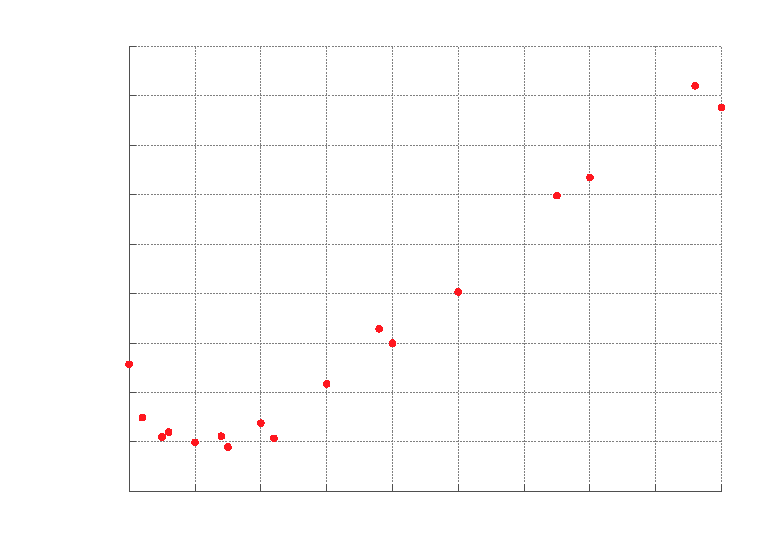
\includegraphics{img/msms/graph-bic-q1}}%
    \gplfronttext
  \end{picture}%
\endgroup
}}
%\subfigure[$Q=2$]{
%\includegraphics[angle=-90,width=0.3\textwidth]{./img/bic2.eps}}
%\resizebox{0.3\textwidth}{!}{\sffamily% GNUPLOT: LaTeX picture with Postscript
\begingroup
  \makeatletter
  \providecommand\color[2][]{%
    \GenericError{(gnuplot) \space\space\space\@spaces}{%
      Package color not loaded in conjunction with
      terminal option `colourtext'%
    }{See the gnuplot documentation for explanation.%
    }{Either use 'blacktext' in gnuplot or load the package
      color.sty in LaTeX.}%
    \renewcommand\color[2][]{}%
  }%
  \providecommand\includegraphics[2][]{%
    \GenericError{(gnuplot) \space\space\space\@spaces}{%
      Package graphicx or graphics not loaded%
    }{See the gnuplot documentation for explanation.%
    }{The gnuplot epslatex terminal needs graphicx.sty or graphics.sty.}%
    \renewcommand\includegraphics[2][]{}%
  }%
  \providecommand\rotatebox[2]{#2}%
  \@ifundefined{ifGPcolor}{%
    \newif\ifGPcolor
    \GPcolortrue
  }{}%
  \@ifundefined{ifGPblacktext}{%
    \newif\ifGPblacktext
    \GPblacktexttrue
  }{}%
  % define a \g@addto@macro without @ in the name:
  \let\gplgaddtomacro\g@addto@macro
  % define empty templates for all commands taking text:
  \gdef\gplbacktext{}%
  \gdef\gplfronttext{}%
  \makeatother
  \ifGPblacktext
    % no textcolor at all
    \def\colorrgb#1{}%
    \def\colorgray#1{}%
  \else
    % gray or color?
    \ifGPcolor
      \def\colorrgb#1{\color[rgb]{#1}}%
      \def\colorgray#1{\color[gray]{#1}}%
      \expandafter\def\csname LTw\endcsname{\color{white}}%
      \expandafter\def\csname LTb\endcsname{\color{black}}%
      \expandafter\def\csname LTa\endcsname{\color{black}}%
      \expandafter\def\csname LT0\endcsname{\color[rgb]{1,0,0}}%
      \expandafter\def\csname LT1\endcsname{\color[rgb]{0,1,0}}%
      \expandafter\def\csname LT2\endcsname{\color[rgb]{0,0,1}}%
      \expandafter\def\csname LT3\endcsname{\color[rgb]{1,0,1}}%
      \expandafter\def\csname LT4\endcsname{\color[rgb]{0,1,1}}%
      \expandafter\def\csname LT5\endcsname{\color[rgb]{1,1,0}}%
      \expandafter\def\csname LT6\endcsname{\color[rgb]{0,0,0}}%
      \expandafter\def\csname LT7\endcsname{\color[rgb]{1,0.3,0}}%
      \expandafter\def\csname LT8\endcsname{\color[rgb]{0.5,0.5,0.5}}%
    \else
      % gray
      \def\colorrgb#1{\color{black}}%
      \def\colorgray#1{\color[gray]{#1}}%
      \expandafter\def\csname LTw\endcsname{\color{white}}%
      \expandafter\def\csname LTb\endcsname{\color{black}}%
      \expandafter\def\csname LTa\endcsname{\color{black}}%
      \expandafter\def\csname LT0\endcsname{\color{black}}%
      \expandafter\def\csname LT1\endcsname{\color{black}}%
      \expandafter\def\csname LT2\endcsname{\color{black}}%
      \expandafter\def\csname LT3\endcsname{\color{black}}%
      \expandafter\def\csname LT4\endcsname{\color{black}}%
      \expandafter\def\csname LT5\endcsname{\color{black}}%
      \expandafter\def\csname LT6\endcsname{\color{black}}%
      \expandafter\def\csname LT7\endcsname{\color{black}}%
      \expandafter\def\csname LT8\endcsname{\color{black}}%
    \fi
  \fi
  \setlength{\unitlength}{0.0500bp}%
  \begin{picture}(7200.00,5040.00)%
    \gplgaddtomacro\gplbacktext{%
      \colorrgb{0.31,0.31,0.31}%
      \put(1080,480){\makebox(0,0)[r]{\strut{}1.2135$\mathsf{\cdot10^6}$}}%
      \colorrgb{0.31,0.31,0.31}%
      \put(1080,1090){\makebox(0,0)[r]{\strut{}1.2136$\mathsf{\cdot10^6}$}}%
      \colorrgb{0.31,0.31,0.31}%
      \put(1080,1700){\makebox(0,0)[r]{\strut{}1.2137$\mathsf{\cdot10^6}$}}%
      \colorrgb{0.31,0.31,0.31}%
      \put(1080,2310){\makebox(0,0)[r]{\strut{}1.2138$\mathsf{\cdot10^6}$}}%
      \colorrgb{0.31,0.31,0.31}%
      \put(1080,2921){\makebox(0,0)[r]{\strut{}1.2139$\mathsf{\cdot10^6}$}}%
      \colorrgb{0.31,0.31,0.31}%
      \put(1080,3531){\makebox(0,0)[r]{\strut{}1.2140$\mathsf{\cdot10^6}$}}%
      \colorrgb{0.31,0.31,0.31}%
      \put(1080,4141){\makebox(0,0)[r]{\strut{}1.2141$\mathsf{\cdot10^6}$}}%
      \colorrgb{0.31,0.31,0.31}%
      \put(1080,4751){\makebox(0,0)[r]{\strut{}1.2142$\mathsf{\cdot10^6}$}}%
      \colorrgb{0.31,0.31,0.31}%
      \put(1224,240){\makebox(0,0){\strut{} 20}}%
      \colorrgb{0.31,0.31,0.31}%
      \put(1917,240){\makebox(0,0){\strut{} 30}}%
      \colorrgb{0.31,0.31,0.31}%
      \put(2610,240){\makebox(0,0){\strut{} 40}}%
      \colorrgb{0.31,0.31,0.31}%
      \put(3303,240){\makebox(0,0){\strut{} 50}}%
      \colorrgb{0.31,0.31,0.31}%
      \put(3995,240){\makebox(0,0){\strut{} 60}}%
      \colorrgb{0.31,0.31,0.31}%
      \put(4688,240){\makebox(0,0){\strut{} 70}}%
      \colorrgb{0.31,0.31,0.31}%
      \put(5381,240){\makebox(0,0){\strut{} 80}}%
      \colorrgb{0.31,0.31,0.31}%
      \put(6074,240){\makebox(0,0){\strut{} 90}}%
      \colorrgb{0.31,0.31,0.31}%
      \put(6767,240){\makebox(0,0){\strut{} 100}}%
    }%
    \gplgaddtomacro\gplfronttext{%
    }%
    \gplbacktext
    \put(0,0){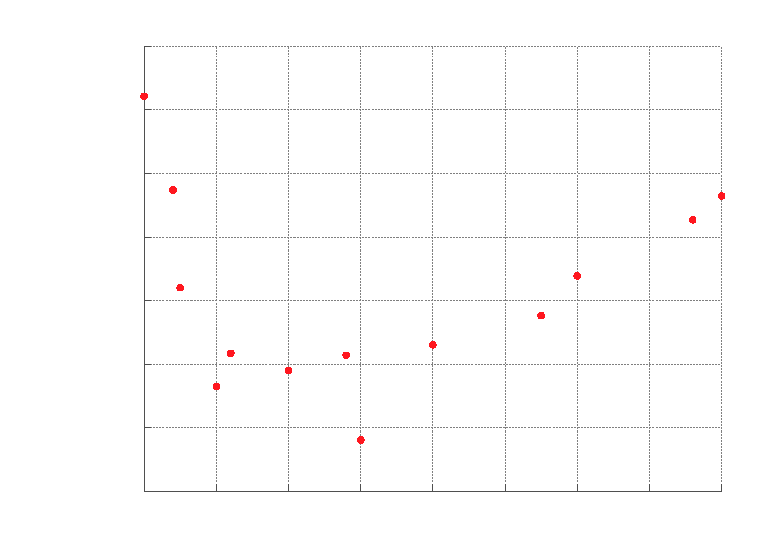
\includegraphics{img/msms/graph-bic-q2}}%
    \gplfronttext
  \end{picture}%
\endgroup
}}
%\subfigure[$Q=3$]{
%\includegraphics[angle=-90,width=0.3\textwidth]{./img/bic3.eps}}
%\resizebox{0.3\textwidth}{!}{\sffamily% GNUPLOT: LaTeX picture with Postscript
\begingroup
  \makeatletter
  \providecommand\color[2][]{%
    \GenericError{(gnuplot) \space\space\space\@spaces}{%
      Package color not loaded in conjunction with
      terminal option `colourtext'%
    }{See the gnuplot documentation for explanation.%
    }{Either use 'blacktext' in gnuplot or load the package
      color.sty in LaTeX.}%
    \renewcommand\color[2][]{}%
  }%
  \providecommand\includegraphics[2][]{%
    \GenericError{(gnuplot) \space\space\space\@spaces}{%
      Package graphicx or graphics not loaded%
    }{See the gnuplot documentation for explanation.%
    }{The gnuplot epslatex terminal needs graphicx.sty or graphics.sty.}%
    \renewcommand\includegraphics[2][]{}%
  }%
  \providecommand\rotatebox[2]{#2}%
  \@ifundefined{ifGPcolor}{%
    \newif\ifGPcolor
    \GPcolortrue
  }{}%
  \@ifundefined{ifGPblacktext}{%
    \newif\ifGPblacktext
    \GPblacktexttrue
  }{}%
  % define a \g@addto@macro without @ in the name:
  \let\gplgaddtomacro\g@addto@macro
  % define empty templates for all commands taking text:
  \gdef\gplbacktext{}%
  \gdef\gplfronttext{}%
  \makeatother
  \ifGPblacktext
    % no textcolor at all
    \def\colorrgb#1{}%
    \def\colorgray#1{}%
  \else
    % gray or color?
    \ifGPcolor
      \def\colorrgb#1{\color[rgb]{#1}}%
      \def\colorgray#1{\color[gray]{#1}}%
      \expandafter\def\csname LTw\endcsname{\color{white}}%
      \expandafter\def\csname LTb\endcsname{\color{black}}%
      \expandafter\def\csname LTa\endcsname{\color{black}}%
      \expandafter\def\csname LT0\endcsname{\color[rgb]{1,0,0}}%
      \expandafter\def\csname LT1\endcsname{\color[rgb]{0,1,0}}%
      \expandafter\def\csname LT2\endcsname{\color[rgb]{0,0,1}}%
      \expandafter\def\csname LT3\endcsname{\color[rgb]{1,0,1}}%
      \expandafter\def\csname LT4\endcsname{\color[rgb]{0,1,1}}%
      \expandafter\def\csname LT5\endcsname{\color[rgb]{1,1,0}}%
      \expandafter\def\csname LT6\endcsname{\color[rgb]{0,0,0}}%
      \expandafter\def\csname LT7\endcsname{\color[rgb]{1,0.3,0}}%
      \expandafter\def\csname LT8\endcsname{\color[rgb]{0.5,0.5,0.5}}%
    \else
      % gray
      \def\colorrgb#1{\color{black}}%
      \def\colorgray#1{\color[gray]{#1}}%
      \expandafter\def\csname LTw\endcsname{\color{white}}%
      \expandafter\def\csname LTb\endcsname{\color{black}}%
      \expandafter\def\csname LTa\endcsname{\color{black}}%
      \expandafter\def\csname LT0\endcsname{\color{black}}%
      \expandafter\def\csname LT1\endcsname{\color{black}}%
      \expandafter\def\csname LT2\endcsname{\color{black}}%
      \expandafter\def\csname LT3\endcsname{\color{black}}%
      \expandafter\def\csname LT4\endcsname{\color{black}}%
      \expandafter\def\csname LT5\endcsname{\color{black}}%
      \expandafter\def\csname LT6\endcsname{\color{black}}%
      \expandafter\def\csname LT7\endcsname{\color{black}}%
      \expandafter\def\csname LT8\endcsname{\color{black}}%
    \fi
  \fi
  \setlength{\unitlength}{0.0500bp}%
  \begin{picture}(7200.00,5040.00)%
    \gplgaddtomacro\gplbacktext{%
      \colorrgb{0.31,0.31,0.31}%
      \put(1080,480){\makebox(0,0)[r]{\strut{}2.6530$\mathsf{\cdot10^6}$}}%
      \colorrgb{0.31,0.31,0.31}%
      \put(1080,955){\makebox(0,0)[r]{\strut{}2.6535$\mathsf{\cdot10^6}$}}%
      \colorrgb{0.31,0.31,0.31}%
      \put(1080,1429){\makebox(0,0)[r]{\strut{}2.6540$\mathsf{\cdot10^6}$}}%
      \colorrgb{0.31,0.31,0.31}%
      \put(1080,1904){\makebox(0,0)[r]{\strut{}2.6545$\mathsf{\cdot10^6}$}}%
      \colorrgb{0.31,0.31,0.31}%
      \put(1080,2378){\makebox(0,0)[r]{\strut{}2.6550$\mathsf{\cdot10^6}$}}%
      \colorrgb{0.31,0.31,0.31}%
      \put(1080,2853){\makebox(0,0)[r]{\strut{}2.6555$\mathsf{\cdot10^6}$}}%
      \colorrgb{0.31,0.31,0.31}%
      \put(1080,3327){\makebox(0,0)[r]{\strut{}2.6560$\mathsf{\cdot10^6}$}}%
      \colorrgb{0.31,0.31,0.31}%
      \put(1080,3802){\makebox(0,0)[r]{\strut{}2.6565$\mathsf{\cdot10^6}$}}%
      \colorrgb{0.31,0.31,0.31}%
      \put(1080,4276){\makebox(0,0)[r]{\strut{}2.6570$\mathsf{\cdot10^6}$}}%
      \colorrgb{0.31,0.31,0.31}%
      \put(1080,4751){\makebox(0,0)[r]{\strut{}2.6575$\mathsf{\cdot10^6}$}}%
      \colorrgb{0.31,0.31,0.31}%
      \put(1224,240){\makebox(0,0){\strut{} 10}}%
      \colorrgb{0.31,0.31,0.31}%
      \put(1840,240){\makebox(0,0){\strut{} 20}}%
      \colorrgb{0.31,0.31,0.31}%
      \put(2456,240){\makebox(0,0){\strut{} 30}}%
      \colorrgb{0.31,0.31,0.31}%
      \put(3072,240){\makebox(0,0){\strut{} 40}}%
      \colorrgb{0.31,0.31,0.31}%
      \put(3688,240){\makebox(0,0){\strut{} 50}}%
      \colorrgb{0.31,0.31,0.31}%
      \put(4303,240){\makebox(0,0){\strut{} 60}}%
      \colorrgb{0.31,0.31,0.31}%
      \put(4919,240){\makebox(0,0){\strut{} 70}}%
      \colorrgb{0.31,0.31,0.31}%
      \put(5535,240){\makebox(0,0){\strut{} 80}}%
      \colorrgb{0.31,0.31,0.31}%
      \put(6151,240){\makebox(0,0){\strut{} 90}}%
      \colorrgb{0.31,0.31,0.31}%
      \put(6767,240){\makebox(0,0){\strut{} 100}}%
    }%
    \gplgaddtomacro\gplfronttext{%
    }%
    \gplbacktext
    \put(0,0){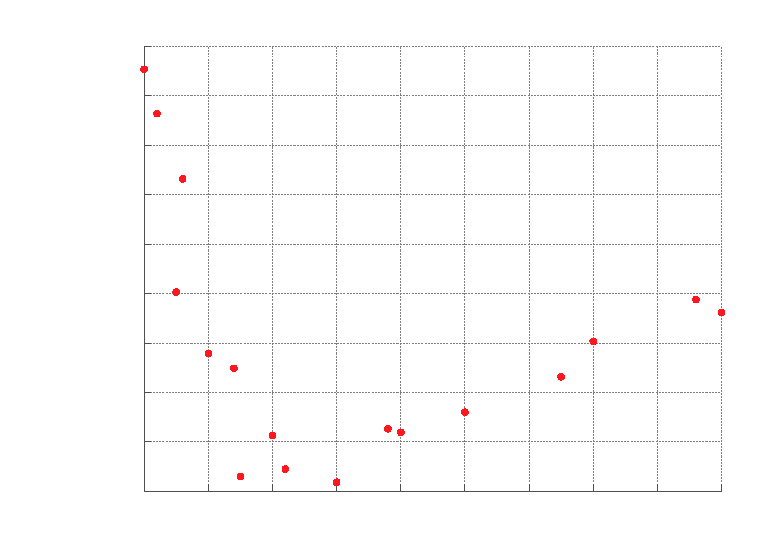
\includegraphics{img/msms/graph-bic-q3}}%
    \gplfronttext
  \end{picture}%
\endgroup
}}\\
\resizebox{0.7\textwidth}{!}{\sffamily% GNUPLOT: LaTeX picture with Postscript
\begingroup
  \makeatletter
  \providecommand\color[2][]{%
    \GenericError{(gnuplot) \space\space\space\@spaces}{%
      Package color not loaded in conjunction with
      terminal option `colourtext'%
    }{See the gnuplot documentation for explanation.%
    }{Either use 'blacktext' in gnuplot or load the package
      color.sty in LaTeX.}%
    \renewcommand\color[2][]{}%
  }%
  \providecommand\includegraphics[2][]{%
    \GenericError{(gnuplot) \space\space\space\@spaces}{%
      Package graphicx or graphics not loaded%
    }{See the gnuplot documentation for explanation.%
    }{The gnuplot epslatex terminal needs graphicx.sty or graphics.sty.}%
    \renewcommand\includegraphics[2][]{}%
  }%
  \providecommand\rotatebox[2]{#2}%
  \@ifundefined{ifGPcolor}{%
    \newif\ifGPcolor
    \GPcolorfalse
  }{}%
  \@ifundefined{ifGPblacktext}{%
    \newif\ifGPblacktext
    \GPblacktexttrue
  }{}%
  % define a \g@addto@macro without @ in the name:
  \let\gplgaddtomacro\g@addto@macro
  % define empty templates for all commands taking text:
  \gdef\gplbacktext{}%
  \gdef\gplfronttext{}%
  \makeatother
  \ifGPblacktext
    % no textcolor at all
    \def\colorrgb#1{}%
    \def\colorgray#1{}%
  \else
    % gray or color?
    \ifGPcolor
      \def\colorrgb#1{\color[rgb]{#1}}%
      \def\colorgray#1{\color[gray]{#1}}%
      \expandafter\def\csname LTw\endcsname{\color{white}}%
      \expandafter\def\csname LTb\endcsname{\color{black}}%
      \expandafter\def\csname LTa\endcsname{\color{black}}%
      \expandafter\def\csname LT0\endcsname{\color[rgb]{1,0,0}}%
      \expandafter\def\csname LT1\endcsname{\color[rgb]{0,1,0}}%
      \expandafter\def\csname LT2\endcsname{\color[rgb]{0,0,1}}%
      \expandafter\def\csname LT3\endcsname{\color[rgb]{1,0,1}}%
      \expandafter\def\csname LT4\endcsname{\color[rgb]{0,1,1}}%
      \expandafter\def\csname LT5\endcsname{\color[rgb]{1,1,0}}%
      \expandafter\def\csname LT6\endcsname{\color[rgb]{0,0,0}}%
      \expandafter\def\csname LT7\endcsname{\color[rgb]{1,0.3,0}}%
      \expandafter\def\csname LT8\endcsname{\color[rgb]{0.5,0.5,0.5}}%
    \else
      % gray
      \def\colorrgb#1{\color{black}}%
      \def\colorgray#1{\color[gray]{#1}}%
      \expandafter\def\csname LTw\endcsname{\color{white}}%
      \expandafter\def\csname LTb\endcsname{\color{black}}%
      \expandafter\def\csname LTa\endcsname{\color{black}}%
      \expandafter\def\csname LT0\endcsname{\color{black}}%
      \expandafter\def\csname LT1\endcsname{\color{black}}%
      \expandafter\def\csname LT2\endcsname{\color{black}}%
      \expandafter\def\csname LT3\endcsname{\color{black}}%
      \expandafter\def\csname LT4\endcsname{\color{black}}%
      \expandafter\def\csname LT5\endcsname{\color{black}}%
      \expandafter\def\csname LT6\endcsname{\color{black}}%
      \expandafter\def\csname LT7\endcsname{\color{black}}%
      \expandafter\def\csname LT8\endcsname{\color{black}}%
    \fi
  \fi
  \setlength{\unitlength}{0.0500bp}%
  \begin{picture}(7200.00,5040.00)%
    \gplgaddtomacro\gplbacktext{%
      \colorrgb{0.31,0.31,0.31}%
      \put(1324,682){\makebox(0,0)[r]{\strut{} 2.6535$\mathsf\cdot10^6$}}%
      \colorrgb{0.31,0.31,0.31}%
      \put(1324,990){\makebox(0,0)[r]{\strut{} 2.6545$\mathsf\cdot10^6$}}%
      \colorrgb{0.31,0.31,0.31}%
      \put(1324,1299){\makebox(0,0)[r]{\strut{} 2.6555$\mathsf\cdot10^6$}}%
      \colorrgb{0.31,0.31,0.31}%
      \put(1324,1607){\makebox(0,0)[r]{\strut{} 2.6565$\mathsf\cdot10^6$}}%
      \colorrgb{0.31,0.31,0.31}%
      \put(1468,288){\makebox(0,0){\strut{} 0}}%
      \colorrgb{0.31,0.31,0.31}%
      \put(2467,288){\makebox(0,0){\strut{} 20}}%
      \colorrgb{0.31,0.31,0.31}%
      \put(3466,288){\makebox(0,0){\strut{} 40}}%
      \colorrgb{0.31,0.31,0.31}%
      \put(4466,288){\makebox(0,0){\strut{} 60}}%
      \colorrgb{0.31,0.31,0.31}%
      \put(5465,288){\makebox(0,0){\strut{} 80}}%
      \colorrgb{0.31,0.31,0.31}%
      \put(6464,288){\makebox(0,0){\strut{} 100}}%
      \csname LTb\endcsname%
      \put(1568,1776){\makebox(0,0)[l]{\strut{}c}}%
    }%
    \gplgaddtomacro\gplfronttext{%
    }%
    \gplgaddtomacro\gplbacktext{%
      \colorrgb{0.31,0.31,0.31}%
      \put(1324,2137){\makebox(0,0)[r]{\strut{} 1.2136$\mathsf\cdot10^7$}}%
      \colorrgb{0.31,0.31,0.31}%
      \put(1324,2533){\makebox(0,0)[r]{\strut{} 1.2138$\mathsf\cdot10^7$}}%
      \colorrgb{0.31,0.31,0.31}%
      \put(1324,2930){\makebox(0,0)[r]{\strut{} 1.2140$\mathsf\cdot10^7$}}%
      \colorrgb{0.31,0.31,0.31}%
      \put(2467,1699){\makebox(0,0){\strut{}}}%
      \colorrgb{0.31,0.31,0.31}%
      \put(3466,1699){\makebox(0,0){\strut{}}}%
      \colorrgb{0.31,0.31,0.31}%
      \put(4466,1699){\makebox(0,0){\strut{}}}%
      \colorrgb{0.31,0.31,0.31}%
      \put(5465,1699){\makebox(0,0){\strut{}}}%
      \csname LTb\endcsname%
      \put(1568,3187){\makebox(0,0)[l]{\strut{}b}}%
    }%
    \gplgaddtomacro\gplfronttext{%
    }%
    \gplgaddtomacro\gplbacktext{%
      \colorrgb{0.31,0.31,0.31}%
      \put(1324,3513){\makebox(0,0)[r]{\strut{} 301600}}%
      \colorrgb{0.31,0.31,0.31}%
      \put(1324,3840){\makebox(0,0)[r]{\strut{} 302000}}%
      \colorrgb{0.31,0.31,0.31}%
      \put(1324,4166){\makebox(0,0)[r]{\strut{} 302400}}%
      \colorrgb{0.31,0.31,0.31}%
      \put(1324,4492){\makebox(0,0)[r]{\strut{} 302800}}%
      \colorrgb{0.31,0.31,0.31}%
      \put(2467,3110){\makebox(0,0){\strut{}}}%
      \colorrgb{0.31,0.31,0.31}%
      \put(3466,3110){\makebox(0,0){\strut{}}}%
      \colorrgb{0.31,0.31,0.31}%
      \put(4466,3110){\makebox(0,0){\strut{}}}%
      \colorrgb{0.31,0.31,0.31}%
      \put(5465,3110){\makebox(0,0){\strut{}}}%
      \csname LTb\endcsname%
      \put(1568,4598){\makebox(0,0)[l]{\strut{}a}}%
    }%
    \gplgaddtomacro\gplfronttext{%
    }%
    \gplbacktext
    \put(0,0){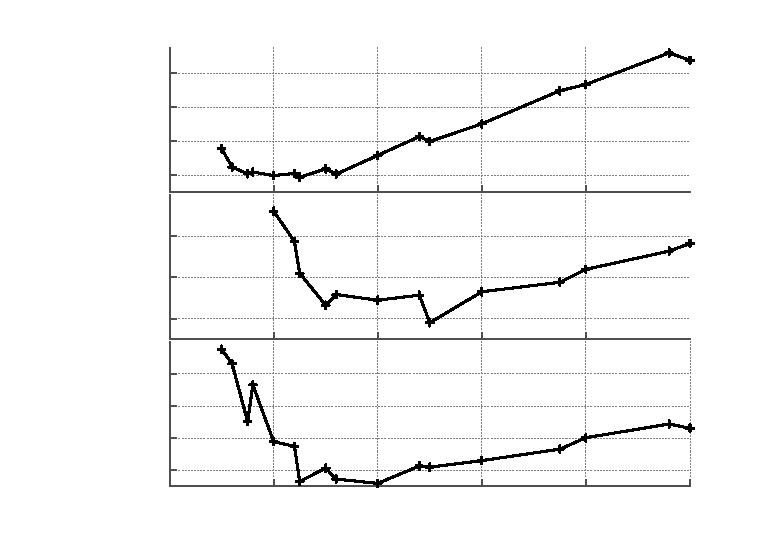
\includegraphics{img/msms/graph-bic}}%
    \gplfronttext
  \end{picture}%
\endgroup
}
\caption{\label{fig:bic}
\emph{Bayesian Information Criterion} (BIC) dependence on the $\tilde\rho$ axis
division $r$. For each value of $r$, a Simulated Annealing
with Montecarlo steps is performed to find the $\tilde I$ axis subdivision that
minimize BIC. The results are reported for different parent charge states: (a)
$Q=1$, (b) $Q=2$ and (c) $Q=3$.}
\end{center}
\end{figure}

Our strategy to choose the best discretization will consist in considering all the models $A_r$; for each of them, 
we will modify the $\tilde I$ discretization independently for each $A_r$, 
finding in each case the binning that minimizes  $B(A_r)$. Finally, we will choose the
model $A^*$ that minimizes the resulting values of
$B(A_r)$ on $r$.
For each $A_r$,  we use a Montecarlo algorithm with Simulated Annealing to
change the binning along the intensity axis and minimize $B(A_r)$. We use the
following  elementary Montecarlo moves
% The Montecarlo step for the minimization of BIC are:
\begin{itemize}
\item move a separation edge up or downward;
\item remove a separation between two bins, joining two contiguous intervals;
\item insert a new division inside a single bin, splitting the interval in two.
\end{itemize}
The results for the minimal BIC obtained at the end of the simulated annealing
procedure for each value of $r$ are reported on figure \ref{fig:bic}.
% and for each $\tilde\rho$
% subdivision report the value of BIC for the optimized $\tilde I$ subdivision.
The global optimized subdivision for each precursor charge  are the following:
\begin{itemize}
% \item $Q=1 \Rightarrow 25$;
% \item $Q=2 \Rightarrow 125$;
% \item $Q=3 \Rightarrow 160$.
 \item $Q=1 \Rightarrow 25$;
 \item $Q=2 \Rightarrow 50$;
 \item $Q=3 \Rightarrow 40$.
\end{itemize}

\begin{figure}[!thb]
\begin{center}
\subfigure[$Q=1$]{
\resizebox{0.4\textwidth}{!}{\sffamily% GNUPLOT: LaTeX picture with Postscript
\begingroup
  \makeatletter
  \providecommand\color[2][]{%
    \GenericError{(gnuplot) \space\space\space\@spaces}{%
      Package color not loaded in conjunction with
      terminal option `colourtext'%
    }{See the gnuplot documentation for explanation.%
    }{Either use 'blacktext' in gnuplot or load the package
      color.sty in LaTeX.}%
    \renewcommand\color[2][]{}%
  }%
  \providecommand\includegraphics[2][]{%
    \GenericError{(gnuplot) \space\space\space\@spaces}{%
      Package graphicx or graphics not loaded%
    }{See the gnuplot documentation for explanation.%
    }{The gnuplot epslatex terminal needs graphicx.sty or graphics.sty.}%
    \renewcommand\includegraphics[2][]{}%
  }%
  \providecommand\rotatebox[2]{#2}%
  \@ifundefined{ifGPcolor}{%
    \newif\ifGPcolor
    \GPcolortrue
  }{}%
  \@ifundefined{ifGPblacktext}{%
    \newif\ifGPblacktext
    \GPblacktexttrue
  }{}%
  % define a \g@addto@macro without @ in the name:
  \let\gplgaddtomacro\g@addto@macro
  % define empty templates for all commands taking text:
  \gdef\gplbacktext{}%
  \gdef\gplfronttext{}%
  \makeatother
  \ifGPblacktext
    % no textcolor at all
    \def\colorrgb#1{}%
    \def\colorgray#1{}%
  \else
    % gray or color?
    \ifGPcolor
      \def\colorrgb#1{\color[rgb]{#1}}%
      \def\colorgray#1{\color[gray]{#1}}%
      \expandafter\def\csname LTw\endcsname{\color{white}}%
      \expandafter\def\csname LTb\endcsname{\color{black}}%
      \expandafter\def\csname LTa\endcsname{\color{black}}%
      \expandafter\def\csname LT0\endcsname{\color[rgb]{1,0,0}}%
      \expandafter\def\csname LT1\endcsname{\color[rgb]{0,1,0}}%
      \expandafter\def\csname LT2\endcsname{\color[rgb]{0,0,1}}%
      \expandafter\def\csname LT3\endcsname{\color[rgb]{1,0,1}}%
      \expandafter\def\csname LT4\endcsname{\color[rgb]{0,1,1}}%
      \expandafter\def\csname LT5\endcsname{\color[rgb]{1,1,0}}%
      \expandafter\def\csname LT6\endcsname{\color[rgb]{0,0,0}}%
      \expandafter\def\csname LT7\endcsname{\color[rgb]{1,0.3,0}}%
      \expandafter\def\csname LT8\endcsname{\color[rgb]{0.5,0.5,0.5}}%
    \else
      % gray
      \def\colorrgb#1{\color{black}}%
      \def\colorgray#1{\color[gray]{#1}}%
      \expandafter\def\csname LTw\endcsname{\color{white}}%
      \expandafter\def\csname LTb\endcsname{\color{black}}%
      \expandafter\def\csname LTa\endcsname{\color{black}}%
      \expandafter\def\csname LT0\endcsname{\color{black}}%
      \expandafter\def\csname LT1\endcsname{\color{black}}%
      \expandafter\def\csname LT2\endcsname{\color{black}}%
      \expandafter\def\csname LT3\endcsname{\color{black}}%
      \expandafter\def\csname LT4\endcsname{\color{black}}%
      \expandafter\def\csname LT5\endcsname{\color{black}}%
      \expandafter\def\csname LT6\endcsname{\color{black}}%
      \expandafter\def\csname LT7\endcsname{\color{black}}%
      \expandafter\def\csname LT8\endcsname{\color{black}}%
    \fi
  \fi
  \setlength{\unitlength}{0.0500bp}%
  \begin{picture}(7200.00,5040.00)%
    \gplgaddtomacro\gplbacktext{%
      \colorrgb{0.31,0.31,0.31}%
      \put(1187,814){\makebox(0,0){\strut{} 0}}%
      \colorrgb{0.31,0.31,0.31}%
      \put(2152,814){\makebox(0,0){\strut{} 0.2}}%
      \colorrgb{0.31,0.31,0.31}%
      \put(3118,814){\makebox(0,0){\strut{} 0.4}}%
      \colorrgb{0.31,0.31,0.31}%
      \put(4082,814){\makebox(0,0){\strut{} 0.6}}%
      \colorrgb{0.31,0.31,0.31}%
      \put(5048,814){\makebox(0,0){\strut{} 0.8}}%
      \colorrgb{0.31,0.31,0.31}%
      \put(6013,814){\makebox(0,0){\strut{} 1}}%
      \colorrgb{0.31,0.31,0.31}%
      \put(1000,1126){\makebox(0,0)[r]{\strut{} 0}}%
      \colorrgb{0.31,0.31,0.31}%
      \put(1000,1732){\makebox(0,0)[r]{\strut{} 0.2}}%
      \colorrgb{0.31,0.31,0.31}%
      \put(1000,2338){\makebox(0,0)[r]{\strut{} 0.4}}%
      \colorrgb{0.31,0.31,0.31}%
      \put(1000,2942){\makebox(0,0)[r]{\strut{} 0.6}}%
      \colorrgb{0.31,0.31,0.31}%
      \put(1000,3548){\makebox(0,0)[r]{\strut{} 0.8}}%
      \colorrgb{0.31,0.31,0.31}%
      \put(1000,4154){\makebox(0,0)[r]{\strut{} 1}}%
    }%
    \gplgaddtomacro\gplfronttext{%
      \colorrgb{0.31,0.31,0.31}%
      \put(6519,1125){\makebox(0,0)[l]{\strut{} 0}}%
      \colorrgb{0.31,0.31,0.31}%
      \put(6519,1503){\makebox(0,0)[l]{\strut{} 0.005}}%
      \colorrgb{0.31,0.31,0.31}%
      \put(6519,1882){\makebox(0,0)[l]{\strut{} 0.01}}%
      \colorrgb{0.31,0.31,0.31}%
      \put(6519,2260){\makebox(0,0)[l]{\strut{} 0.015}}%
      \colorrgb{0.31,0.31,0.31}%
      \put(6519,2639){\makebox(0,0)[l]{\strut{} 0.02}}%
      \colorrgb{0.31,0.31,0.31}%
      \put(6519,3018){\makebox(0,0)[l]{\strut{} 0.025}}%
      \colorrgb{0.31,0.31,0.31}%
      \put(6519,3396){\makebox(0,0)[l]{\strut{} 0.03}}%
      \colorrgb{0.31,0.31,0.31}%
      \put(6519,3775){\makebox(0,0)[l]{\strut{} 0.035}}%
      \colorrgb{0.31,0.31,0.31}%
      \put(6519,4154){\makebox(0,0)[l]{\strut{} 0.04}}%
    }%
    \gplbacktext
    \put(0,0){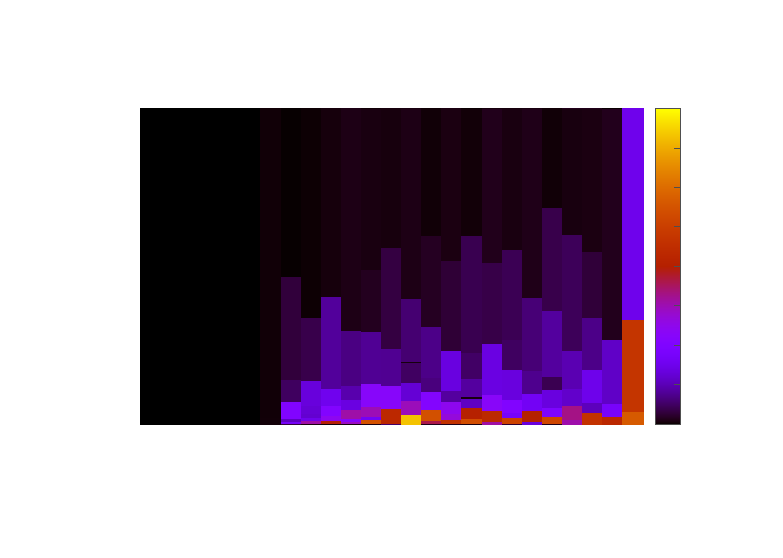
\includegraphics{img/msms/graph-dist-tot-q1}}%
    \gplfronttext
  \end{picture}%
\endgroup
}}
%\includegraphics[angle=-90,width=0.4\textwidth]{./img/img-grid-q1.eps}}
\subfigure[$Q=2$]{
\resizebox{0.4\textwidth}{!}{\sffamily% GNUPLOT: LaTeX picture with Postscript
\begingroup
  \makeatletter
  \providecommand\color[2][]{%
    \GenericError{(gnuplot) \space\space\space\@spaces}{%
      Package color not loaded in conjunction with
      terminal option `colourtext'%
    }{See the gnuplot documentation for explanation.%
    }{Either use 'blacktext' in gnuplot or load the package
      color.sty in LaTeX.}%
    \renewcommand\color[2][]{}%
  }%
  \providecommand\includegraphics[2][]{%
    \GenericError{(gnuplot) \space\space\space\@spaces}{%
      Package graphicx or graphics not loaded%
    }{See the gnuplot documentation for explanation.%
    }{The gnuplot epslatex terminal needs graphicx.sty or graphics.sty.}%
    \renewcommand\includegraphics[2][]{}%
  }%
  \providecommand\rotatebox[2]{#2}%
  \@ifundefined{ifGPcolor}{%
    \newif\ifGPcolor
    \GPcolortrue
  }{}%
  \@ifundefined{ifGPblacktext}{%
    \newif\ifGPblacktext
    \GPblacktexttrue
  }{}%
  % define a \g@addto@macro without @ in the name:
  \let\gplgaddtomacro\g@addto@macro
  % define empty templates for all commands taking text:
  \gdef\gplbacktext{}%
  \gdef\gplfronttext{}%
  \makeatother
  \ifGPblacktext
    % no textcolor at all
    \def\colorrgb#1{}%
    \def\colorgray#1{}%
  \else
    % gray or color?
    \ifGPcolor
      \def\colorrgb#1{\color[rgb]{#1}}%
      \def\colorgray#1{\color[gray]{#1}}%
      \expandafter\def\csname LTw\endcsname{\color{white}}%
      \expandafter\def\csname LTb\endcsname{\color{black}}%
      \expandafter\def\csname LTa\endcsname{\color{black}}%
      \expandafter\def\csname LT0\endcsname{\color[rgb]{1,0,0}}%
      \expandafter\def\csname LT1\endcsname{\color[rgb]{0,1,0}}%
      \expandafter\def\csname LT2\endcsname{\color[rgb]{0,0,1}}%
      \expandafter\def\csname LT3\endcsname{\color[rgb]{1,0,1}}%
      \expandafter\def\csname LT4\endcsname{\color[rgb]{0,1,1}}%
      \expandafter\def\csname LT5\endcsname{\color[rgb]{1,1,0}}%
      \expandafter\def\csname LT6\endcsname{\color[rgb]{0,0,0}}%
      \expandafter\def\csname LT7\endcsname{\color[rgb]{1,0.3,0}}%
      \expandafter\def\csname LT8\endcsname{\color[rgb]{0.5,0.5,0.5}}%
    \else
      % gray
      \def\colorrgb#1{\color{black}}%
      \def\colorgray#1{\color[gray]{#1}}%
      \expandafter\def\csname LTw\endcsname{\color{white}}%
      \expandafter\def\csname LTb\endcsname{\color{black}}%
      \expandafter\def\csname LTa\endcsname{\color{black}}%
      \expandafter\def\csname LT0\endcsname{\color{black}}%
      \expandafter\def\csname LT1\endcsname{\color{black}}%
      \expandafter\def\csname LT2\endcsname{\color{black}}%
      \expandafter\def\csname LT3\endcsname{\color{black}}%
      \expandafter\def\csname LT4\endcsname{\color{black}}%
      \expandafter\def\csname LT5\endcsname{\color{black}}%
      \expandafter\def\csname LT6\endcsname{\color{black}}%
      \expandafter\def\csname LT7\endcsname{\color{black}}%
      \expandafter\def\csname LT8\endcsname{\color{black}}%
    \fi
  \fi
  \setlength{\unitlength}{0.0500bp}%
  \begin{picture}(7200.00,5040.00)%
    \gplgaddtomacro\gplbacktext{%
      \colorrgb{0.31,0.31,0.31}%
      \put(1187,814){\makebox(0,0){\strut{} 0}}%
      \colorrgb{0.31,0.31,0.31}%
      \put(2152,814){\makebox(0,0){\strut{} 0.2}}%
      \colorrgb{0.31,0.31,0.31}%
      \put(3118,814){\makebox(0,0){\strut{} 0.4}}%
      \colorrgb{0.31,0.31,0.31}%
      \put(4082,814){\makebox(0,0){\strut{} 0.6}}%
      \colorrgb{0.31,0.31,0.31}%
      \put(5048,814){\makebox(0,0){\strut{} 0.8}}%
      \colorrgb{0.31,0.31,0.31}%
      \put(6013,814){\makebox(0,0){\strut{} 1}}%
      \colorrgb{0.31,0.31,0.31}%
      \put(1000,1126){\makebox(0,0)[r]{\strut{} 0}}%
      \colorrgb{0.31,0.31,0.31}%
      \put(1000,1732){\makebox(0,0)[r]{\strut{} 0.2}}%
      \colorrgb{0.31,0.31,0.31}%
      \put(1000,2338){\makebox(0,0)[r]{\strut{} 0.4}}%
      \colorrgb{0.31,0.31,0.31}%
      \put(1000,2942){\makebox(0,0)[r]{\strut{} 0.6}}%
      \colorrgb{0.31,0.31,0.31}%
      \put(1000,3548){\makebox(0,0)[r]{\strut{} 0.8}}%
      \colorrgb{0.31,0.31,0.31}%
      \put(1000,4154){\makebox(0,0)[r]{\strut{} 1}}%
    }%
    \gplgaddtomacro\gplfronttext{%
      \colorrgb{0.31,0.31,0.31}%
      \put(6519,1125){\makebox(0,0)[l]{\strut{} 0}}%
      \colorrgb{0.31,0.31,0.31}%
      \put(6519,1557){\makebox(0,0)[l]{\strut{} 0.002}}%
      \colorrgb{0.31,0.31,0.31}%
      \put(6519,1990){\makebox(0,0)[l]{\strut{} 0.004}}%
      \colorrgb{0.31,0.31,0.31}%
      \put(6519,2423){\makebox(0,0)[l]{\strut{} 0.006}}%
      \colorrgb{0.31,0.31,0.31}%
      \put(6519,2855){\makebox(0,0)[l]{\strut{} 0.008}}%
      \colorrgb{0.31,0.31,0.31}%
      \put(6519,3288){\makebox(0,0)[l]{\strut{} 0.01}}%
      \colorrgb{0.31,0.31,0.31}%
      \put(6519,3721){\makebox(0,0)[l]{\strut{} 0.012}}%
      \colorrgb{0.31,0.31,0.31}%
      \put(6519,4154){\makebox(0,0)[l]{\strut{} 0.014}}%
    }%
    \gplbacktext
    \put(0,0){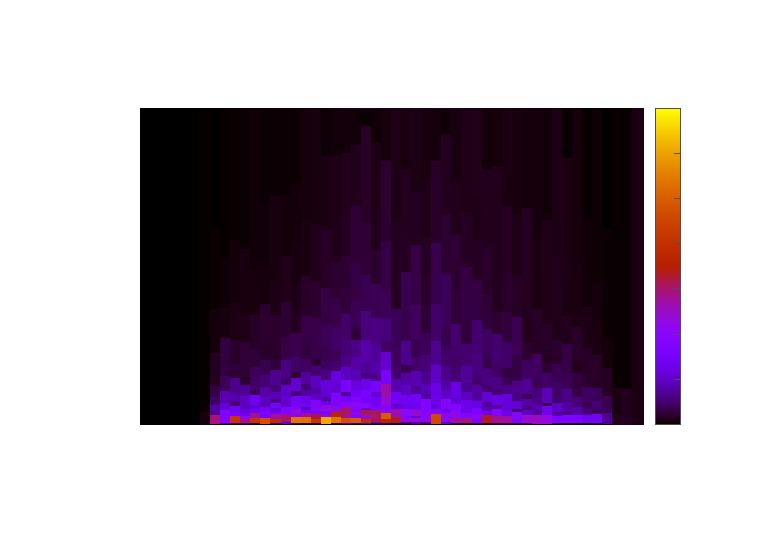
\includegraphics{img/msms/graph-dist-tot-q2}}%
    \gplfronttext
  \end{picture}%
\endgroup
}}
%\includegraphics[angle=-90,width=0.4\textwidth]{./img/img-grid-q2.eps}}
\subfigure[$Q=3$]{
\resizebox{0.4\textwidth}{!}{\sffamily% GNUPLOT: LaTeX picture with Postscript
\begingroup
  \makeatletter
  \providecommand\color[2][]{%
    \GenericError{(gnuplot) \space\space\space\@spaces}{%
      Package color not loaded in conjunction with
      terminal option `colourtext'%
    }{See the gnuplot documentation for explanation.%
    }{Either use 'blacktext' in gnuplot or load the package
      color.sty in LaTeX.}%
    \renewcommand\color[2][]{}%
  }%
  \providecommand\includegraphics[2][]{%
    \GenericError{(gnuplot) \space\space\space\@spaces}{%
      Package graphicx or graphics not loaded%
    }{See the gnuplot documentation for explanation.%
    }{The gnuplot epslatex terminal needs graphicx.sty or graphics.sty.}%
    \renewcommand\includegraphics[2][]{}%
  }%
  \providecommand\rotatebox[2]{#2}%
  \@ifundefined{ifGPcolor}{%
    \newif\ifGPcolor
    \GPcolortrue
  }{}%
  \@ifundefined{ifGPblacktext}{%
    \newif\ifGPblacktext
    \GPblacktexttrue
  }{}%
  % define a \g@addto@macro without @ in the name:
  \let\gplgaddtomacro\g@addto@macro
  % define empty templates for all commands taking text:
  \gdef\gplbacktext{}%
  \gdef\gplfronttext{}%
  \makeatother
  \ifGPblacktext
    % no textcolor at all
    \def\colorrgb#1{}%
    \def\colorgray#1{}%
  \else
    % gray or color?
    \ifGPcolor
      \def\colorrgb#1{\color[rgb]{#1}}%
      \def\colorgray#1{\color[gray]{#1}}%
      \expandafter\def\csname LTw\endcsname{\color{white}}%
      \expandafter\def\csname LTb\endcsname{\color{black}}%
      \expandafter\def\csname LTa\endcsname{\color{black}}%
      \expandafter\def\csname LT0\endcsname{\color[rgb]{1,0,0}}%
      \expandafter\def\csname LT1\endcsname{\color[rgb]{0,1,0}}%
      \expandafter\def\csname LT2\endcsname{\color[rgb]{0,0,1}}%
      \expandafter\def\csname LT3\endcsname{\color[rgb]{1,0,1}}%
      \expandafter\def\csname LT4\endcsname{\color[rgb]{0,1,1}}%
      \expandafter\def\csname LT5\endcsname{\color[rgb]{1,1,0}}%
      \expandafter\def\csname LT6\endcsname{\color[rgb]{0,0,0}}%
      \expandafter\def\csname LT7\endcsname{\color[rgb]{1,0.3,0}}%
      \expandafter\def\csname LT8\endcsname{\color[rgb]{0.5,0.5,0.5}}%
    \else
      % gray
      \def\colorrgb#1{\color{black}}%
      \def\colorgray#1{\color[gray]{#1}}%
      \expandafter\def\csname LTw\endcsname{\color{white}}%
      \expandafter\def\csname LTb\endcsname{\color{black}}%
      \expandafter\def\csname LTa\endcsname{\color{black}}%
      \expandafter\def\csname LT0\endcsname{\color{black}}%
      \expandafter\def\csname LT1\endcsname{\color{black}}%
      \expandafter\def\csname LT2\endcsname{\color{black}}%
      \expandafter\def\csname LT3\endcsname{\color{black}}%
      \expandafter\def\csname LT4\endcsname{\color{black}}%
      \expandafter\def\csname LT5\endcsname{\color{black}}%
      \expandafter\def\csname LT6\endcsname{\color{black}}%
      \expandafter\def\csname LT7\endcsname{\color{black}}%
      \expandafter\def\csname LT8\endcsname{\color{black}}%
    \fi
  \fi
  \setlength{\unitlength}{0.0500bp}%
  \begin{picture}(7200.00,5040.00)%
    \gplgaddtomacro\gplbacktext{%
      \colorrgb{0.31,0.31,0.31}%
      \put(1187,814){\makebox(0,0){\strut{} 0}}%
      \colorrgb{0.31,0.31,0.31}%
      \put(2152,814){\makebox(0,0){\strut{} 0.2}}%
      \colorrgb{0.31,0.31,0.31}%
      \put(3118,814){\makebox(0,0){\strut{} 0.4}}%
      \colorrgb{0.31,0.31,0.31}%
      \put(4082,814){\makebox(0,0){\strut{} 0.6}}%
      \colorrgb{0.31,0.31,0.31}%
      \put(5048,814){\makebox(0,0){\strut{} 0.8}}%
      \colorrgb{0.31,0.31,0.31}%
      \put(6013,814){\makebox(0,0){\strut{} 1}}%
      \colorrgb{0.31,0.31,0.31}%
      \put(1000,1126){\makebox(0,0)[r]{\strut{} 0}}%
      \colorrgb{0.31,0.31,0.31}%
      \put(1000,1732){\makebox(0,0)[r]{\strut{} 0.2}}%
      \colorrgb{0.31,0.31,0.31}%
      \put(1000,2338){\makebox(0,0)[r]{\strut{} 0.4}}%
      \colorrgb{0.31,0.31,0.31}%
      \put(1000,2942){\makebox(0,0)[r]{\strut{} 0.6}}%
      \colorrgb{0.31,0.31,0.31}%
      \put(1000,3548){\makebox(0,0)[r]{\strut{} 0.8}}%
      \colorrgb{0.31,0.31,0.31}%
      \put(1000,4154){\makebox(0,0)[r]{\strut{} 1}}%
    }%
    \gplgaddtomacro\gplfronttext{%
      \colorrgb{0.31,0.31,0.31}%
      \put(6519,1125){\makebox(0,0)[l]{\strut{} 0}}%
      \colorrgb{0.31,0.31,0.31}%
      \put(6519,1629){\makebox(0,0)[l]{\strut{} 0.005}}%
      \colorrgb{0.31,0.31,0.31}%
      \put(6519,2134){\makebox(0,0)[l]{\strut{} 0.01}}%
      \colorrgb{0.31,0.31,0.31}%
      \put(6519,2639){\makebox(0,0)[l]{\strut{} 0.015}}%
      \colorrgb{0.31,0.31,0.31}%
      \put(6519,3144){\makebox(0,0)[l]{\strut{} 0.02}}%
      \colorrgb{0.31,0.31,0.31}%
      \put(6519,3649){\makebox(0,0)[l]{\strut{} 0.025}}%
      \colorrgb{0.31,0.31,0.31}%
      \put(6519,4154){\makebox(0,0)[l]{\strut{} 0.03}}%
    }%
    \gplbacktext
    \put(0,0){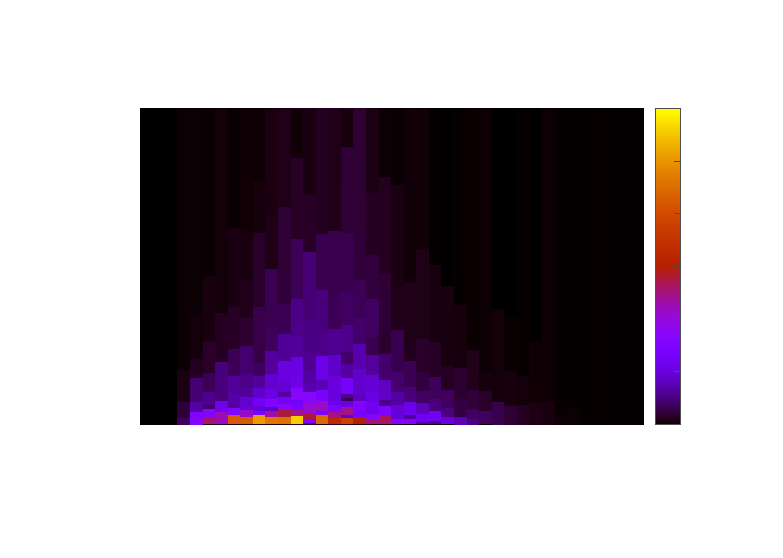
\includegraphics{img/msms/graph-dist-tot-q3}}%
    \gplfronttext
  \end{picture}%
\endgroup
}}
%\includegraphics[angle=-90,width=0.4\textwidth]{./img/img-grid-q2.eps}}
\caption{\label{fig:peaks-dist}
Total peaks distribution in the three different parent charge state. The peaks
distribution is described in the $[0:1]\otimes[0:1]$ space, subdivided in
intervals according to BIC criterion in order to minimize the number of
parameters without loosing quality of fit.The results are reported for different
parent charge states: (a) $Q=1$, (b) $Q=2$ and (c) $Q=3$.}
\end{center}
\end{figure}

%-----------------------------------------------------------------------------
\section{Selection of Significant Ions}
%-----------------------------------------------------------------------------
\label{sec:shannon}

%The peaks where collected in three different databases, depending on parent charge
%state $Q$, in the renormalized form. In this way all peaks are represented by
%couples of variables $(\tilde\rho\in]0:1],\tilde I\in]0:1])$ and tags which
%describe the peak interpretation based on the theoretical sequence of the
%peptide provided by Sequest.

In tandem mass spectroscopy not all the fragments are produced with the same
probability: the most frequently observed peaks are mono-charged $b$ and $y$
and, among neutral losses, those of water or ammonia are the most expressed.
We want to select between all type of possible product ions a significant subset
that is critical to reveal the presence of a fragmentation site.
%Peaks tagging is cleaned of non-significative states: $c-NH_3 = b, z = y-NH_3,
%+wat-wat = 0$.


To this end, we analyse the amount of information the presence of a certain type of product ion conveys.
We follow a strategy similar to that proposed by \citet{gygi2004nature} %and references therein, 
in which reduction of Shannon Entropy was used to learn from the database the importance in term of information of each kind of fragment.

\emph{Shannon Entropy} \cite{shannon1948} is a measure of the
information content of a random variable or more precisely the uncertainty
associated to it.
%We can write the total amount of Shannon Entropy of the entire system as:
We introduce a model of the system with discrete variables, describing the
distribution of the peaks on plane divided in a finite number of bins.
The \emph{Shannon Entropy} $H$ of the model $A^*(Q)$ that represents the
distribution of peaks from peptides with charge $Q$, can be defined as
\begin{equation}
 H(A^*(Q))=-\sum_{\alpha\in A^*(Q)} p(\alpha)\log_2 p(\alpha)
\label{eq:shannon}
\end{equation}
where the sum is performed over the model bins, and $p(\alpha)$ is the fraction
of peaks falling inside the bin $\alpha$.
The separation of the original set of peaks into two subsets increases the
information content with the classification of those peaks, the result of such
operation can be described with a decrease in the entropy of the entire system.
The Shannon Entropy of a general system separated into $A$ non-overlapping
subsets can be written as:
\begin{equation}
 H(\alpha|A)=-\sum_A p(A)\sum_\alpha p(\alpha|A)\log_2 p(\alpha|A)
\end{equation}

The strategy relies on the computation of the entropy decrease due
to the recognition/separation of a type of fragment $s_i$ (identified by fragment family,
$a,b,c$ or $x,y,z$, its charge $q$ and its neutral losses $\bm l$) from the rest
of peaks.
We calculate, then, the Shannon Entropy of the two non-overlapping subsets
$\Sigma_{s_i}\equiv\{s_i\in\Sigma\}$, that gather the $s_i$
peaks,
and the complementary $\Sigma\setminus\Sigma_{s_i}$.
Using Eq.~\ref{eq:shannon}, this became:
\begin{align}
%H(\Sigma)&=
%H(A^*(Q))\\
H(\Sigma_{s_i})&=
\sum_\alpha p(\alpha|s_i)\log_2 p(\alpha|s_i)\\
H(\Sigma\setminus\Sigma_{s_i})&=
\sum_\alpha p(\alpha|\bar s_i)\log_2 p(\alpha|\bar s_i)
\end{align}
where $p(\alpha|s_i)$ and $p(\alpha|\bar s_i)$ represent the distributions of the
$s_i$ peaks and of all but $s_i$ peaks respectively.
The entropy loss $\Delta H(s_i)$ due to the separation/recognition of
$s_i$ peaks shows the amount of information gained and can be written as:
\begin{equation}
\Delta H (s_i) = p(\Sigma)H(\Sigma)
	-p(\Sigma_{s_i})H(\Sigma_{s_i})
	-p(\Sigma\setminus\Sigma_{s_i})H(\Sigma\setminus\Sigma_{s_i})
\end{equation}
where $H(\Sigma)$ is calculated as in Eq.~\ref{eq:shannon}, $p(X)$ is the
fraction of peaks that belong to $X$.

We consider the fragment type $s_i$ that yield the greatest entropy loss by
maximizing $\Delta H(s_i)$ and remove it from the total set of peaks.
We then repeat the operation over the remaining peaks.
In this way, we obtained the list of product ion types reported in Table \ref{tab:list}, ranked according to their information content.
In the case that a peak matches two fragments, it is assigned to the one with the higher entropy loss.

Fig.~\ref{fig:spec-entropy} shows the picture of the entropy loss at every
fragment type separation.
Notice that the recognition of the firsts few ion types provide the greatest
increase in information retrieval, with an high value of entropy loss.
\begin{figure}
\centering
%\includegraphics[width=4cm,angle=-90]{./img/msms/list-Dentropy.eps}
\resizebox{0.6\textwidth}{!}{\sffamily% GNUPLOT: LaTeX picture with Postscript
\begingroup
  \makeatletter
  \providecommand\color[2][]{%
    \GenericError{(gnuplot) \space\space\space\@spaces}{%
      Package color not loaded in conjunction with
      terminal option `colourtext'%
    }{See the gnuplot documentation for explanation.%
    }{Either use 'blacktext' in gnuplot or load the package
      color.sty in LaTeX.}%
    \renewcommand\color[2][]{}%
  }%
  \providecommand\includegraphics[2][]{%
    \GenericError{(gnuplot) \space\space\space\@spaces}{%
      Package graphicx or graphics not loaded%
    }{See the gnuplot documentation for explanation.%
    }{The gnuplot epslatex terminal needs graphicx.sty or graphics.sty.}%
    \renewcommand\includegraphics[2][]{}%
  }%
  \providecommand\rotatebox[2]{#2}%
  \@ifundefined{ifGPcolor}{%
    \newif\ifGPcolor
    \GPcolortrue
  }{}%
  \@ifundefined{ifGPblacktext}{%
    \newif\ifGPblacktext
    \GPblacktexttrue
  }{}%
  % define a \g@addto@macro without @ in the name:
  \let\gplgaddtomacro\g@addto@macro
  % define empty templates for all commands taking text:
  \gdef\gplbacktext{}%
  \gdef\gplfronttext{}%
  \makeatother
  \ifGPblacktext
    % no textcolor at all
    \def\colorrgb#1{}%
    \def\colorgray#1{}%
  \else
    % gray or color?
    \ifGPcolor
      \def\colorrgb#1{\color[rgb]{#1}}%
      \def\colorgray#1{\color[gray]{#1}}%
      \expandafter\def\csname LTw\endcsname{\color{white}}%
      \expandafter\def\csname LTb\endcsname{\color{black}}%
      \expandafter\def\csname LTa\endcsname{\color{black}}%
      \expandafter\def\csname LT0\endcsname{\color[rgb]{1,0,0}}%
      \expandafter\def\csname LT1\endcsname{\color[rgb]{0,1,0}}%
      \expandafter\def\csname LT2\endcsname{\color[rgb]{0,0,1}}%
      \expandafter\def\csname LT3\endcsname{\color[rgb]{1,0,1}}%
      \expandafter\def\csname LT4\endcsname{\color[rgb]{0,1,1}}%
      \expandafter\def\csname LT5\endcsname{\color[rgb]{1,1,0}}%
      \expandafter\def\csname LT6\endcsname{\color[rgb]{0,0,0}}%
      \expandafter\def\csname LT7\endcsname{\color[rgb]{1,0.3,0}}%
      \expandafter\def\csname LT8\endcsname{\color[rgb]{0.5,0.5,0.5}}%
    \else
      % gray
      \def\colorrgb#1{\color{black}}%
      \def\colorgray#1{\color[gray]{#1}}%
      \expandafter\def\csname LTw\endcsname{\color{white}}%
      \expandafter\def\csname LTb\endcsname{\color{black}}%
      \expandafter\def\csname LTa\endcsname{\color{black}}%
      \expandafter\def\csname LT0\endcsname{\color{black}}%
      \expandafter\def\csname LT1\endcsname{\color{black}}%
      \expandafter\def\csname LT2\endcsname{\color{black}}%
      \expandafter\def\csname LT3\endcsname{\color{black}}%
      \expandafter\def\csname LT4\endcsname{\color{black}}%
      \expandafter\def\csname LT5\endcsname{\color{black}}%
      \expandafter\def\csname LT6\endcsname{\color{black}}%
      \expandafter\def\csname LT7\endcsname{\color{black}}%
      \expandafter\def\csname LT8\endcsname{\color{black}}%
    \fi
  \fi
  \setlength{\unitlength}{0.0500bp}%
  \begin{picture}(7200.00,5040.00)%
    \gplgaddtomacro\gplbacktext{%
      \colorrgb{0.31,0.31,0.31}%
      \put(1176,768){\makebox(0,0)[r]{\strut{} 0}}%
      \colorrgb{0.31,0.31,0.31}%
      \put(1176,1337){\makebox(0,0)[r]{\strut{} 0.01}}%
      \colorrgb{0.31,0.31,0.31}%
      \put(1176,1906){\makebox(0,0)[r]{\strut{} 0.02}}%
      \colorrgb{0.31,0.31,0.31}%
      \put(1176,2475){\makebox(0,0)[r]{\strut{} 0.03}}%
      \colorrgb{0.31,0.31,0.31}%
      \put(1176,3044){\makebox(0,0)[r]{\strut{} 0.04}}%
      \colorrgb{0.31,0.31,0.31}%
      \put(1176,3613){\makebox(0,0)[r]{\strut{} 0.05}}%
      \colorrgb{0.31,0.31,0.31}%
      \put(1176,4182){\makebox(0,0)[r]{\strut{} 0.06}}%
      \colorrgb{0.31,0.31,0.31}%
      \put(1176,4751){\makebox(0,0)[r]{\strut{} 0.07}}%
      \colorrgb{0.31,0.31,0.31}%
      \put(1815,528){\makebox(0,0){\strut{}1}}%
      \colorrgb{0.31,0.31,0.31}%
      \put(2310,528){\makebox(0,0){\strut{}2}}%
      \colorrgb{0.31,0.31,0.31}%
      \put(2806,528){\makebox(0,0){\strut{}3}}%
      \colorrgb{0.31,0.31,0.31}%
      \put(3301,528){\makebox(0,0){\strut{}4}}%
      \colorrgb{0.31,0.31,0.31}%
      \put(3796,528){\makebox(0,0){\strut{}5}}%
      \colorrgb{0.31,0.31,0.31}%
      \put(4291,528){\makebox(0,0){\strut{}6}}%
      \colorrgb{0.31,0.31,0.31}%
      \put(4786,528){\makebox(0,0){\strut{}7}}%
      \colorrgb{0.31,0.31,0.31}%
      \put(5281,528){\makebox(0,0){\strut{}8}}%
      \colorrgb{0.31,0.31,0.31}%
      \put(5777,528){\makebox(0,0){\strut{}9}}%
      \colorrgb{0.31,0.31,0.31}%
      \put(6272,528){\makebox(0,0){\strut{}10}}%
      \csname LTb\endcsname%
      \put(192,2759){\rotatebox{-270}{\makebox(0,0){\strut{}$\Delta$S}}}%
      \put(4043,168){\makebox(0,0){\strut{}species}}%
    }%
    \gplgaddtomacro\gplfronttext{%
      \csname LTb\endcsname%
      \put(5696,4568){\makebox(0,0)[r]{\strut{}Q=1}}%
      \csname LTb\endcsname%
      \put(5696,4328){\makebox(0,0)[r]{\strut{}Q=2}}%
      \csname LTb\endcsname%
      \put(5696,4088){\makebox(0,0)[r]{\strut{}Q=3}}%
    }%
    \gplbacktext
    \put(0,0){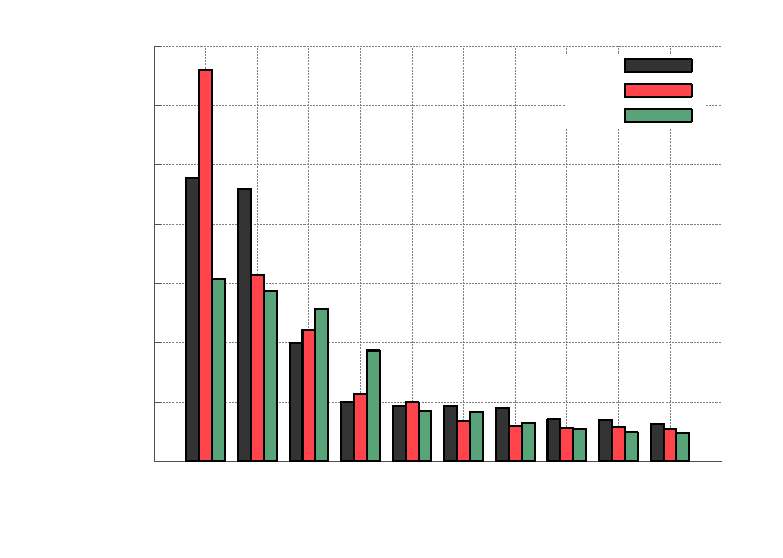
\includegraphics{img/msms/graph-shannon}}%
    \gplfronttext
  \end{picture}%
\endgroup
}
\caption{\label{fig:spec-entropy}
Entropy reduction due to interpretation and consequently separation of each
species from the rest of peaks. Most of the information is carried by the first 
few ion species where generally higher positions are occupied by $y$ and $b$
ions, usually with double charged ions or ions with losses of water or ammonia.}
\end{figure}


\begin{table}
\begin{center}
\footnotesize
\begin{tabular}{crlrlrl}
\hline \hline
seq & \multicolumn{2}{c}{$Q=1$}&
\multicolumn{2}{c}{$Q=2$}&\multicolumn{2}{c}{$Q=3$}\\
&  fragment & N & fragment & N & fragment & N \\
\hline
1 & $y		$& 1173 & $y 		$&  50208  &$ y++	        $&  6812\\
2 & $b 		$& 1003 & $b 		$&  43842  &$ y 		$&  6776\\
3 & $b-H_2O 	$&  546 & $y++ 		$&  14224  &$ b++		$&  4723\\
4 & $a  	$&  515 & $y-NH3++ 	$&   9825  &$ b			$&  5705\\
5 & $y-H_2O 	$&  369 & $b-wat 	$&  21252  &$ b-H_2O++   	$&  2445\\
6 & $b-2H_2O 	$&  233 & $y-H_2O-NH_3++$&   6081  &$ y-NH_3++   	$&  3536\\
7 & $y-NH_3 	$&  556 & $y-H_2O 	$&  13385  &$ b-H_2O-NH_3++	$&  1044\\
8 & $c 		$&  321 & $x++		$&   6641  &$ a++       	$&  2096\\
9 & $b-NH_3 	$&  143 & $x-NH_3++	$&   6546  &$ y-H_2O-NH_3++	$&  1798\\
10 & $b+H_2O 	$&  129 & $y-H_2O++	$&   4654  &$ b-H_2O-NH_3++	$&  1161\\
%1 & $y		$& 8993 & y 		& 213072  & y++		& 90944\\
%2 & $b 		$& 8015 & b 		& 196393  & y 		& 78465\\
%3 & $b-H_2O 	$& 4966 & y++ 		& 79900   & b++		& 59528\\
%4 & $y-NH_3 	$& 5153 & y-NH3++ 	& 69875   & b		& 72112\\
%5 & $y-H_2O 	$& 3461 & b-wat 		& 107453  & y-NH3++	& 70046\\
%6 & $b-NH_3 	$& 2163 & x++ 		& 57759   & b-NH3++	& 42909\\
%7 & $b-2H_2O 	$& 1929 & x-NH3++ 	& 56292   & a++		& 39141\\
%8 & $a 		$& 4212 & y-wat-NH3++	& 46004   & b-wat-NH3++	& 29175\\
%9 & $a-H_2O 	$& 2494 & z-wat-NH3++	& 41035   & y-wat-NH3++	& 42920\\
%10 & $b-H_2O-NH_3 	$& 1109 & x-wat-NH3++	& 42757   & x-wat++	& 40144\\
%11 & $b-NH_3+H_2O 	$& 302  & b-NH3		& 55430   & z-wat-NH3++	& 38922\\
%12 & $y-H_2O-NH_3 	$& 2539 & y-wat		& 73303   & x-wat-NH3++	& 39006\\
%13 & $b+H_2O 	$& 725  & y-wat++	& 28965   & x++		& 48382\\
%14 & $c	 	$& 2855 & b++		& 21849   & c++		& 31335\\
%15 & $y-H_2O-H_2O	$& 1159 & y-NH3		& 103916  & a-wat++	& 26366\\
\hline \hline
\end{tabular}
\caption{\label{tab:list}
Ranked list of product ion types, according to the associated \emph{Shannon
Entropy} loss. The latter represents the missing information or unpredictability of
the random variable, so that the entropy loss can be interpreted as information gain upon their identification. 
Remarkably, the list reports as top significant those ions that are usually used for spectra identification.
%highly ordering ions those already accepted as most frequently observed.
}
\end{center}
\end{table}

\begin{figure}[!thb]
\begin{center}
\subfigure[matched]{
%\includegraphics[angle=-90, width=0.45\textwidth]{./img/y_q2_match.eps}}
\resizebox{0.45\textwidth}{!}{\sffamily% GNUPLOT: LaTeX picture with Postscript
\begingroup
  \makeatletter
  \providecommand\color[2][]{%
    \GenericError{(gnuplot) \space\space\space\@spaces}{%
      Package color not loaded in conjunction with
      terminal option `colourtext'%
    }{See the gnuplot documentation for explanation.%
    }{Either use 'blacktext' in gnuplot or load the package
      color.sty in LaTeX.}%
    \renewcommand\color[2][]{}%
  }%
  \providecommand\includegraphics[2][]{%
    \GenericError{(gnuplot) \space\space\space\@spaces}{%
      Package graphicx or graphics not loaded%
    }{See the gnuplot documentation for explanation.%
    }{The gnuplot epslatex terminal needs graphicx.sty or graphics.sty.}%
    \renewcommand\includegraphics[2][]{}%
  }%
  \providecommand\rotatebox[2]{#2}%
  \@ifundefined{ifGPcolor}{%
    \newif\ifGPcolor
    \GPcolortrue
  }{}%
  \@ifundefined{ifGPblacktext}{%
    \newif\ifGPblacktext
    \GPblacktexttrue
  }{}%
  % define a \g@addto@macro without @ in the name:
  \let\gplgaddtomacro\g@addto@macro
  % define empty templates for all commands taking text:
  \gdef\gplbacktext{}%
  \gdef\gplfronttext{}%
  \makeatother
  \ifGPblacktext
    % no textcolor at all
    \def\colorrgb#1{}%
    \def\colorgray#1{}%
  \else
    % gray or color?
    \ifGPcolor
      \def\colorrgb#1{\color[rgb]{#1}}%
      \def\colorgray#1{\color[gray]{#1}}%
      \expandafter\def\csname LTw\endcsname{\color{white}}%
      \expandafter\def\csname LTb\endcsname{\color{black}}%
      \expandafter\def\csname LTa\endcsname{\color{black}}%
      \expandafter\def\csname LT0\endcsname{\color[rgb]{1,0,0}}%
      \expandafter\def\csname LT1\endcsname{\color[rgb]{0,1,0}}%
      \expandafter\def\csname LT2\endcsname{\color[rgb]{0,0,1}}%
      \expandafter\def\csname LT3\endcsname{\color[rgb]{1,0,1}}%
      \expandafter\def\csname LT4\endcsname{\color[rgb]{0,1,1}}%
      \expandafter\def\csname LT5\endcsname{\color[rgb]{1,1,0}}%
      \expandafter\def\csname LT6\endcsname{\color[rgb]{0,0,0}}%
      \expandafter\def\csname LT7\endcsname{\color[rgb]{1,0.3,0}}%
      \expandafter\def\csname LT8\endcsname{\color[rgb]{0.5,0.5,0.5}}%
    \else
      % gray
      \def\colorrgb#1{\color{black}}%
      \def\colorgray#1{\color[gray]{#1}}%
      \expandafter\def\csname LTw\endcsname{\color{white}}%
      \expandafter\def\csname LTb\endcsname{\color{black}}%
      \expandafter\def\csname LTa\endcsname{\color{black}}%
      \expandafter\def\csname LT0\endcsname{\color{black}}%
      \expandafter\def\csname LT1\endcsname{\color{black}}%
      \expandafter\def\csname LT2\endcsname{\color{black}}%
      \expandafter\def\csname LT3\endcsname{\color{black}}%
      \expandafter\def\csname LT4\endcsname{\color{black}}%
      \expandafter\def\csname LT5\endcsname{\color{black}}%
      \expandafter\def\csname LT6\endcsname{\color{black}}%
      \expandafter\def\csname LT7\endcsname{\color{black}}%
      \expandafter\def\csname LT8\endcsname{\color{black}}%
    \fi
  \fi
  \setlength{\unitlength}{0.0500bp}%
  \begin{picture}(7200.00,5040.00)%
    \gplgaddtomacro\gplbacktext{%
      \colorrgb{0.31,0.31,0.31}%
      \put(1187,814){\makebox(0,0){\strut{} 0}}%
      \colorrgb{0.31,0.31,0.31}%
      \put(2152,814){\makebox(0,0){\strut{} 0.2}}%
      \colorrgb{0.31,0.31,0.31}%
      \put(3118,814){\makebox(0,0){\strut{} 0.4}}%
      \colorrgb{0.31,0.31,0.31}%
      \put(4082,814){\makebox(0,0){\strut{} 0.6}}%
      \colorrgb{0.31,0.31,0.31}%
      \put(5048,814){\makebox(0,0){\strut{} 0.8}}%
      \colorrgb{0.31,0.31,0.31}%
      \put(6013,814){\makebox(0,0){\strut{} 1}}%
      \colorrgb{0.31,0.31,0.31}%
      \put(1000,1126){\makebox(0,0)[r]{\strut{} 0}}%
      \colorrgb{0.31,0.31,0.31}%
      \put(1000,1732){\makebox(0,0)[r]{\strut{} 0.2}}%
      \colorrgb{0.31,0.31,0.31}%
      \put(1000,2338){\makebox(0,0)[r]{\strut{} 0.4}}%
      \colorrgb{0.31,0.31,0.31}%
      \put(1000,2942){\makebox(0,0)[r]{\strut{} 0.6}}%
      \colorrgb{0.31,0.31,0.31}%
      \put(1000,3548){\makebox(0,0)[r]{\strut{} 0.8}}%
      \colorrgb{0.31,0.31,0.31}%
      \put(1000,4154){\makebox(0,0)[r]{\strut{} 1}}%
    }%
    \gplgaddtomacro\gplfronttext{%
      \colorrgb{0.31,0.31,0.31}%
      \put(6519,1125){\makebox(0,0)[l]{\strut{} 0}}%
      \colorrgb{0.31,0.31,0.31}%
      \put(6519,1427){\makebox(0,0)[l]{\strut{} 0.0005}}%
      \colorrgb{0.31,0.31,0.31}%
      \put(6519,1730){\makebox(0,0)[l]{\strut{} 0.001}}%
      \colorrgb{0.31,0.31,0.31}%
      \put(6519,2033){\makebox(0,0)[l]{\strut{} 0.0015}}%
      \colorrgb{0.31,0.31,0.31}%
      \put(6519,2336){\makebox(0,0)[l]{\strut{} 0.002}}%
      \colorrgb{0.31,0.31,0.31}%
      \put(6519,2639){\makebox(0,0)[l]{\strut{} 0.0025}}%
      \colorrgb{0.31,0.31,0.31}%
      \put(6519,2942){\makebox(0,0)[l]{\strut{} 0.003}}%
      \colorrgb{0.31,0.31,0.31}%
      \put(6519,3245){\makebox(0,0)[l]{\strut{} 0.0035}}%
      \colorrgb{0.31,0.31,0.31}%
      \put(6519,3548){\makebox(0,0)[l]{\strut{} 0.004}}%
      \colorrgb{0.31,0.31,0.31}%
      \put(6519,3851){\makebox(0,0)[l]{\strut{} 0.0045}}%
      \colorrgb{0.31,0.31,0.31}%
      \put(6519,4154){\makebox(0,0)[l]{\strut{} 0.005}}%
    }%
    \gplbacktext
    \put(0,0){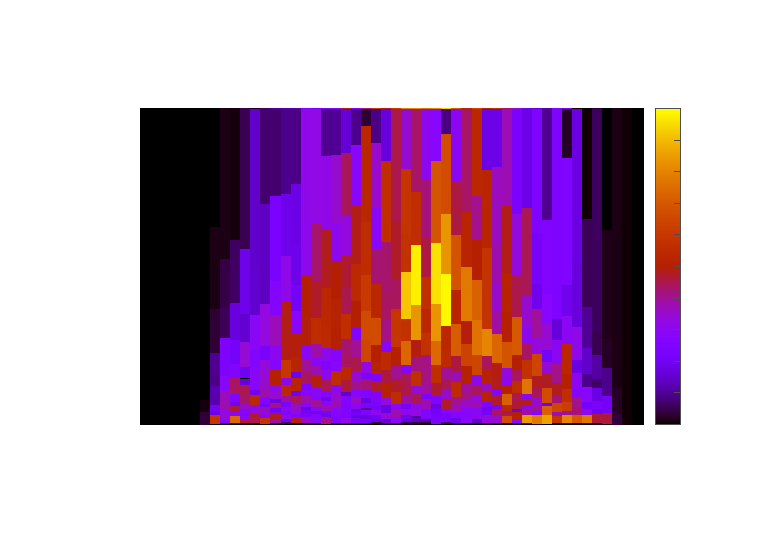
\includegraphics{img/msms/graph-dist-match-q2}}%
    \gplfronttext
  \end{picture}%
\endgroup
}}
\subfigure[unmatched]{
%\includegraphics[angle=-90, width=0.45\textwidth]{./img/y_q2_unmatch.eps}}
\resizebox{0.45\textwidth}{!}{\sffamily% GNUPLOT: LaTeX picture with Postscript
\begingroup
  \makeatletter
  \providecommand\color[2][]{%
    \GenericError{(gnuplot) \space\space\space\@spaces}{%
      Package color not loaded in conjunction with
      terminal option `colourtext'%
    }{See the gnuplot documentation for explanation.%
    }{Either use 'blacktext' in gnuplot or load the package
      color.sty in LaTeX.}%
    \renewcommand\color[2][]{}%
  }%
  \providecommand\includegraphics[2][]{%
    \GenericError{(gnuplot) \space\space\space\@spaces}{%
      Package graphicx or graphics not loaded%
    }{See the gnuplot documentation for explanation.%
    }{The gnuplot epslatex terminal needs graphicx.sty or graphics.sty.}%
    \renewcommand\includegraphics[2][]{}%
  }%
  \providecommand\rotatebox[2]{#2}%
  \@ifundefined{ifGPcolor}{%
    \newif\ifGPcolor
    \GPcolortrue
  }{}%
  \@ifundefined{ifGPblacktext}{%
    \newif\ifGPblacktext
    \GPblacktexttrue
  }{}%
  % define a \g@addto@macro without @ in the name:
  \let\gplgaddtomacro\g@addto@macro
  % define empty templates for all commands taking text:
  \gdef\gplbacktext{}%
  \gdef\gplfronttext{}%
  \makeatother
  \ifGPblacktext
    % no textcolor at all
    \def\colorrgb#1{}%
    \def\colorgray#1{}%
  \else
    % gray or color?
    \ifGPcolor
      \def\colorrgb#1{\color[rgb]{#1}}%
      \def\colorgray#1{\color[gray]{#1}}%
      \expandafter\def\csname LTw\endcsname{\color{white}}%
      \expandafter\def\csname LTb\endcsname{\color{black}}%
      \expandafter\def\csname LTa\endcsname{\color{black}}%
      \expandafter\def\csname LT0\endcsname{\color[rgb]{1,0,0}}%
      \expandafter\def\csname LT1\endcsname{\color[rgb]{0,1,0}}%
      \expandafter\def\csname LT2\endcsname{\color[rgb]{0,0,1}}%
      \expandafter\def\csname LT3\endcsname{\color[rgb]{1,0,1}}%
      \expandafter\def\csname LT4\endcsname{\color[rgb]{0,1,1}}%
      \expandafter\def\csname LT5\endcsname{\color[rgb]{1,1,0}}%
      \expandafter\def\csname LT6\endcsname{\color[rgb]{0,0,0}}%
      \expandafter\def\csname LT7\endcsname{\color[rgb]{1,0.3,0}}%
      \expandafter\def\csname LT8\endcsname{\color[rgb]{0.5,0.5,0.5}}%
    \else
      % gray
      \def\colorrgb#1{\color{black}}%
      \def\colorgray#1{\color[gray]{#1}}%
      \expandafter\def\csname LTw\endcsname{\color{white}}%
      \expandafter\def\csname LTb\endcsname{\color{black}}%
      \expandafter\def\csname LTa\endcsname{\color{black}}%
      \expandafter\def\csname LT0\endcsname{\color{black}}%
      \expandafter\def\csname LT1\endcsname{\color{black}}%
      \expandafter\def\csname LT2\endcsname{\color{black}}%
      \expandafter\def\csname LT3\endcsname{\color{black}}%
      \expandafter\def\csname LT4\endcsname{\color{black}}%
      \expandafter\def\csname LT5\endcsname{\color{black}}%
      \expandafter\def\csname LT6\endcsname{\color{black}}%
      \expandafter\def\csname LT7\endcsname{\color{black}}%
      \expandafter\def\csname LT8\endcsname{\color{black}}%
    \fi
  \fi
  \setlength{\unitlength}{0.0500bp}%
  \begin{picture}(7200.00,5040.00)%
    \gplgaddtomacro\gplbacktext{%
      \colorrgb{0.31,0.31,0.31}%
      \put(1187,814){\makebox(0,0){\strut{} 0}}%
      \colorrgb{0.31,0.31,0.31}%
      \put(2152,814){\makebox(0,0){\strut{} 0.2}}%
      \colorrgb{0.31,0.31,0.31}%
      \put(3118,814){\makebox(0,0){\strut{} 0.4}}%
      \colorrgb{0.31,0.31,0.31}%
      \put(4082,814){\makebox(0,0){\strut{} 0.6}}%
      \colorrgb{0.31,0.31,0.31}%
      \put(5048,814){\makebox(0,0){\strut{} 0.8}}%
      \colorrgb{0.31,0.31,0.31}%
      \put(6013,814){\makebox(0,0){\strut{} 1}}%
      \colorrgb{0.31,0.31,0.31}%
      \put(1000,1126){\makebox(0,0)[r]{\strut{} 0}}%
      \colorrgb{0.31,0.31,0.31}%
      \put(1000,1732){\makebox(0,0)[r]{\strut{} 0.2}}%
      \colorrgb{0.31,0.31,0.31}%
      \put(1000,2338){\makebox(0,0)[r]{\strut{} 0.4}}%
      \colorrgb{0.31,0.31,0.31}%
      \put(1000,2942){\makebox(0,0)[r]{\strut{} 0.6}}%
      \colorrgb{0.31,0.31,0.31}%
      \put(1000,3548){\makebox(0,0)[r]{\strut{} 0.8}}%
      \colorrgb{0.31,0.31,0.31}%
      \put(1000,4154){\makebox(0,0)[r]{\strut{} 1}}%
    }%
    \gplgaddtomacro\gplfronttext{%
      \colorrgb{0.31,0.31,0.31}%
      \put(6519,1125){\makebox(0,0)[l]{\strut{} 0}}%
      \colorrgb{0.31,0.31,0.31}%
      \put(6519,1557){\makebox(0,0)[l]{\strut{} 0.002}}%
      \colorrgb{0.31,0.31,0.31}%
      \put(6519,1990){\makebox(0,0)[l]{\strut{} 0.004}}%
      \colorrgb{0.31,0.31,0.31}%
      \put(6519,2423){\makebox(0,0)[l]{\strut{} 0.006}}%
      \colorrgb{0.31,0.31,0.31}%
      \put(6519,2855){\makebox(0,0)[l]{\strut{} 0.008}}%
      \colorrgb{0.31,0.31,0.31}%
      \put(6519,3288){\makebox(0,0)[l]{\strut{} 0.01}}%
      \colorrgb{0.31,0.31,0.31}%
      \put(6519,3721){\makebox(0,0)[l]{\strut{} 0.012}}%
      \colorrgb{0.31,0.31,0.31}%
      \put(6519,4154){\makebox(0,0)[l]{\strut{} 0.014}}%
    }%
    \gplbacktext
    \put(0,0){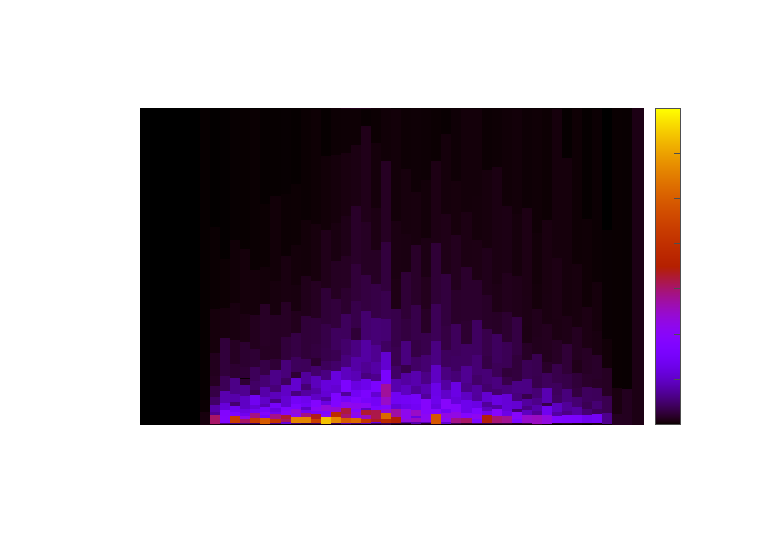
\includegraphics{img/msms/graph-dist-unmatch-q2}}%
    \gplfronttext
  \end{picture}%
\endgroup
}}\\
\caption{\label{fig:dist-ex}
Example of distribution in the normalized and discretized space. The example represents
the distribution of peaks corresponding to $y$-ions (a), and the distribution of
the remaining peaks, after the separation (b).}
\end{center}
\end{figure}

It is remarkable that the usually observed peaks in a general spectrum, and the
ions that present higher peaks intensity in experiments, are top ranking on the
ordered list of Table \ref{tab:list}.

%%%%%%%%%%%%%%%%%%%%%%%%%%%%%%%%%%%%%%%%%%%%%%%%%%%%%%%%%%%%%%%%%%%%%%%%%%%%
\subsection{Missing Peaks}

\begin{figure}[!thb]
\begin{center}
\ \\
%\includegraphics[angle=-90,width=0.5\textwidth]{./img/msms/express_ratio.eps}
\resizebox{0.6\textwidth}{!}{\sffamily% GNUPLOT: LaTeX picture with Postscript
\begingroup
  \makeatletter
  \providecommand\color[2][]{%
    \GenericError{(gnuplot) \space\space\space\@spaces}{%
      Package color not loaded in conjunction with
      terminal option `colourtext'%
    }{See the gnuplot documentation for explanation.%
    }{Either use 'blacktext' in gnuplot or load the package
      color.sty in LaTeX.}%
    \renewcommand\color[2][]{}%
  }%
  \providecommand\includegraphics[2][]{%
    \GenericError{(gnuplot) \space\space\space\@spaces}{%
      Package graphicx or graphics not loaded%
    }{See the gnuplot documentation for explanation.%
    }{The gnuplot epslatex terminal needs graphicx.sty or graphics.sty.}%
    \renewcommand\includegraphics[2][]{}%
  }%
  \providecommand\rotatebox[2]{#2}%
  \@ifundefined{ifGPcolor}{%
    \newif\ifGPcolor
    \GPcolorfalse
  }{}%
  \@ifundefined{ifGPblacktext}{%
    \newif\ifGPblacktext
    \GPblacktexttrue
  }{}%
  % define a \g@addto@macro without @ in the name:
  \let\gplgaddtomacro\g@addto@macro
  % define empty templates for all commands taking text:
  \gdef\gplbacktext{}%
  \gdef\gplfronttext{}%
  \makeatother
  \ifGPblacktext
    % no textcolor at all
    \def\colorrgb#1{}%
    \def\colorgray#1{}%
  \else
    % gray or color?
    \ifGPcolor
      \def\colorrgb#1{\color[rgb]{#1}}%
      \def\colorgray#1{\color[gray]{#1}}%
      \expandafter\def\csname LTw\endcsname{\color{white}}%
      \expandafter\def\csname LTb\endcsname{\color{black}}%
      \expandafter\def\csname LTa\endcsname{\color{black}}%
      \expandafter\def\csname LT0\endcsname{\color[rgb]{1,0,0}}%
      \expandafter\def\csname LT1\endcsname{\color[rgb]{0,1,0}}%
      \expandafter\def\csname LT2\endcsname{\color[rgb]{0,0,1}}%
      \expandafter\def\csname LT3\endcsname{\color[rgb]{1,0,1}}%
      \expandafter\def\csname LT4\endcsname{\color[rgb]{0,1,1}}%
      \expandafter\def\csname LT5\endcsname{\color[rgb]{1,1,0}}%
      \expandafter\def\csname LT6\endcsname{\color[rgb]{0,0,0}}%
      \expandafter\def\csname LT7\endcsname{\color[rgb]{1,0.3,0}}%
      \expandafter\def\csname LT8\endcsname{\color[rgb]{0.5,0.5,0.5}}%
    \else
      % gray
      \def\colorrgb#1{\color{black}}%
      \def\colorgray#1{\color[gray]{#1}}%
      \expandafter\def\csname LTw\endcsname{\color{white}}%
      \expandafter\def\csname LTb\endcsname{\color{black}}%
      \expandafter\def\csname LTa\endcsname{\color{black}}%
      \expandafter\def\csname LT0\endcsname{\color{black}}%
      \expandafter\def\csname LT1\endcsname{\color{black}}%
      \expandafter\def\csname LT2\endcsname{\color{black}}%
      \expandafter\def\csname LT3\endcsname{\color{black}}%
      \expandafter\def\csname LT4\endcsname{\color{black}}%
      \expandafter\def\csname LT5\endcsname{\color{black}}%
      \expandafter\def\csname LT6\endcsname{\color{black}}%
      \expandafter\def\csname LT7\endcsname{\color{black}}%
      \expandafter\def\csname LT8\endcsname{\color{black}}%
    \fi
  \fi
  \setlength{\unitlength}{0.0500bp}%
  \begin{picture}(7200.00,5040.00)%
    \gplgaddtomacro\gplbacktext{%
      \colorrgb{0.31,0.31,0.31}%
      \put(288,4032){\makebox(0,0)[r]{\strut{} 0.2}}%
      \colorrgb{0.31,0.31,0.31}%
      \put(288,4284){\makebox(0,0)[r]{\strut{} 0.4}}%
      \colorrgb{0.31,0.31,0.31}%
      \put(288,4535){\makebox(0,0)[r]{\strut{} 0.6}}%
      \colorrgb{0.31,0.31,0.31}%
      \put(288,4787){\makebox(0,0)[r]{\strut{} 0.8}}%
      \colorrgb{0.31,0.31,0.31}%
      \put(288,5039){\makebox(0,0)[r]{\strut{} 1}}%
    }%
    \gplgaddtomacro\gplfronttext{%
    }%
    \gplgaddtomacro\gplbacktext{%
      \colorrgb{0.31,0.31,0.31}%
      \put(288,2772){\makebox(0,0)[r]{\strut{} 0.2}}%
      \colorrgb{0.31,0.31,0.31}%
      \put(288,3024){\makebox(0,0)[r]{\strut{} 0.4}}%
      \colorrgb{0.31,0.31,0.31}%
      \put(288,3275){\makebox(0,0)[r]{\strut{} 0.6}}%
      \colorrgb{0.31,0.31,0.31}%
      \put(288,3527){\makebox(0,0)[r]{\strut{} 0.8}}%
      \colorrgb{0.31,0.31,0.31}%
      \put(288,3779){\makebox(0,0)[r]{\strut{} 1}}%
    }%
    \gplgaddtomacro\gplfronttext{%
    }%
    \gplgaddtomacro\gplbacktext{%
      \colorrgb{0.31,0.31,0.31}%
      \put(288,1260){\makebox(0,0)[r]{\strut{} 0}}%
      \colorrgb{0.31,0.31,0.31}%
      \put(288,1512){\makebox(0,0)[r]{\strut{} 0.2}}%
      \colorrgb{0.31,0.31,0.31}%
      \put(288,1764){\makebox(0,0)[r]{\strut{} 0.4}}%
      \colorrgb{0.31,0.31,0.31}%
      \put(288,2016){\makebox(0,0)[r]{\strut{} 0.6}}%
      \colorrgb{0.31,0.31,0.31}%
      \put(288,2268){\makebox(0,0)[r]{\strut{} 0.8}}%
      \colorrgb{0.31,0.31,0.31}%
      \put(288,2520){\makebox(0,0)[r]{\strut{} 1}}%
      \colorrgb{0.31,0.31,0.31}%
      \put(432,1020){\makebox(0,0){\strut{} 0}}%
      \colorrgb{0.31,0.31,0.31}%
      \put(1066,1020){\makebox(0,0){\strut{} 0.1}}%
      \colorrgb{0.31,0.31,0.31}%
      \put(1699,1020){\makebox(0,0){\strut{} 0.2}}%
      \colorrgb{0.31,0.31,0.31}%
      \put(2333,1020){\makebox(0,0){\strut{} 0.3}}%
      \colorrgb{0.31,0.31,0.31}%
      \put(2966,1020){\makebox(0,0){\strut{} 0.4}}%
      \colorrgb{0.31,0.31,0.31}%
      \put(3600,1020){\makebox(0,0){\strut{} 0.5}}%
      \colorrgb{0.31,0.31,0.31}%
      \put(4233,1020){\makebox(0,0){\strut{} 0.6}}%
      \colorrgb{0.31,0.31,0.31}%
      \put(4867,1020){\makebox(0,0){\strut{} 0.7}}%
      \colorrgb{0.31,0.31,0.31}%
      \put(5500,1020){\makebox(0,0){\strut{} 0.8}}%
      \colorrgb{0.31,0.31,0.31}%
      \put(6133,1020){\makebox(0,0){\strut{} 0.9}}%
      \colorrgb{0.31,0.31,0.31}%
      \put(6767,1020){\makebox(0,0){\strut{} 1}}%
      \csname LTb\endcsname%
      \put(3599,660){\makebox(0,0){\strut{}$\rho$}}%
    }%
    \gplgaddtomacro\gplfronttext{%
    }%
    \gplbacktext
    \put(0,0){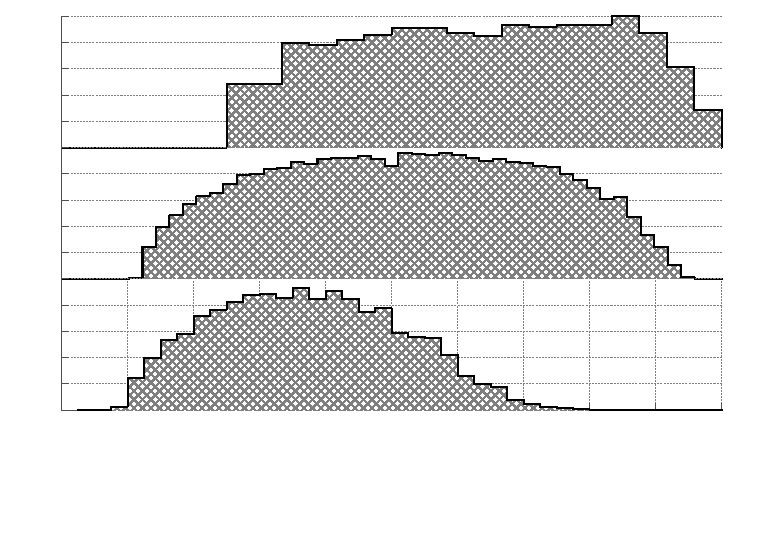
\includegraphics{img/msms/multi-y-expression}}%
    \gplfronttext
  \end{picture}%
\endgroup
}
\end{center}
\vskip -15pt
\caption{\label{fig:y-int-dist}
Example of the fraction of $y$ ion expressed in those spectra,
for peptides with charge $Q=1$ (top), $Q=2$ (centre) and $Q=3$ (bottom), as a
function of $\tilde\rho\in]0:1]$.}
\end{figure}



Low energy CID fragments the precursor peptide on the peptide bonds but not all
the expected ions are expressed on the resulting spectrum. The presence of
Proline (P), the three-dimensional structure of the
peptide entering the fragmentation chamber as well as other factors, may influence the
fragmentation pattern and yield one or several missing peaks.

It is  then possible that some expected theoretical peaks, calculated from the
parent peptide sequence associated to any spectrum of the database, 
do not match any  experimental peak in the
spectrum, yielding ``missing'' or ``ghost'' peaks, i.e., 
peaks with null intensity.


Figure \ref{fig:y-int-dist} describes the distribution of the expressed fraction
of $y$ fragments as function of $\tilde\rho$, for doubly charged peptides.
The figure shows the instrument limitation at low values of mass-to-charge
ratio $\rho$, while near the peptide centre almost every expected $y$ ion
match at least a peak in the corresponding spectrum.
The ``pit'' at the centre of the spectrum with lower expression fraction  
is due to a post-processing of the output data: in a small window around the
precursor ions peaks are removed, if the precursor is double-charged then this
window fall in the centre of the spectrum.


%%%%%%%%%%%%%%%%%%%%%%%%%%%%%%%%%%%%%%%%%%%%%%%%%%%%%%%%%%%%
%%%%%%%%%%%%%%%%%%%%%%%%%%%%%%%%%%%%%%%%%%%%%%%%%%%%%%%%%%%%
\chapter{Defining the Potential}
\label{chap:pot}
\nopagebreak
%%%%%%%%%%%%%%%%%%%%%%%%%%%%%%%%%%%%%%%%%%%%%%%%%%%%%%%%%%%%
%%%%%%%%%%%%%%%%%%%%%%%%%%%%%%%%%%%%%%%%%%%%%%%%%%%%%%%%%%%%



In Chapter~\ref{chap:alg}, we have seen that it is possible to map all the
possible sequences with the correct total mass on the configurations of a
physical model with discrete variables defined on a one-dimensional lattice. We
have also seen that, provided the (potential) energy of the system has an
appropriate simple form, it is possible to solve the equilibrium of the system
and calculate the most likely configuration at low temperature, representing the
best parent sequence, and other thermodynamic variables that can be used to
estimate the quality of the identification.
It is clear that in such approach, the choice of the potential function, to be
used as a score for the proposed sequence, is crucial, and different functions
can yield very different performances of the overall methods. How should this
potential be chosen?


\section{Definitions and statement of the problem}

To answer appropriately to this question, let us start by considering the
process of spectra production: the ensemble of identical (and unknown) parent
peptides $P*$ undergo Collision Induced Dissociation, which acts as a
statistical process, generating a spectrum of ``true'' peaks. Meanwhile, a noise
source $R^\Sigma$, that in principle may be different for different samples and
different spectra, adds up more peaks, again with an unknown statistical
distribution.

Let us call  $\Sigma=\{\pi_\alpha,\alpha=1,\dots,\mathcal N_\Sigma\}$  the total
resulting spectrum, as the collection of $\mathcal N_\Sigma$ peaks
$\pi_\alpha=(\rho_\alpha,I_\alpha)$  with mass-to-charge ratio $\rho_\alpha$ and
observed intensity $I_\alpha$

To estimate the probability that a proposed sequence $P$ is indeed the true
precursor ion $P*$, we need to compare the theoretical spectrum associated to
$P$ with the experimental one.





The set of theoretical peaks expected in the fragmentation of %the proposed peptide
$P$ depends, in our description, on the location $\nu_k$ of the peptide bonds of
the precursor peptide in our one-dimensional lattice description: let $\mathcal
F(P)= \{\nu_k,k=1,\dots,L-1\}$, be the set of the possible fragmentation
positions of $P$,  with $L$ is the length in residues of $P$;
$\nu_k$ is equal to  the sum of the discretized masses of
the sequence residues up to $k$. 
 
Let $\mathcal T_\nu=\{s_i(\nu),i=1,\dots,N_s\}$ be the set of the
peaks produced by all kind of fragmentations at the peptide bond located  at
$\nu$, with  $N_s$ the number of expected type of ions per peptide bond,
while $\mathcal T=\{\mathcal T_{\nu_k},k=1,\dots,L-1\}$ is 
the total set of peaks that can be obtained from  $P$.
Notice that $N_s$ depends in general on the fragmentation site, since the number
of possible peaks depends on the presence and on the position, in the sequence
$P$, of residues that can be charged or can undergo neutral losses. In our
description (see Section~\ref{sec:hamiltonian}), $N_s$ will depend on the state variable
$\sigma_\nu$: $N_s^\nu(\sigma_\nu)$.


\begin{figure}[!thb]
\begin{center}
\psfrag{T}{$\Theta$}
\psfrag{S}{$\Sigma$}
\psfrag{S'}{$\Sigma'$}
\psfrag{S-S'}{$\Sigma\setminus\Sigma'$}
\psfrag{A}{A}
\psfrag{B}{B}
\psfrag{C}{C}
\psfrag{D}{D}
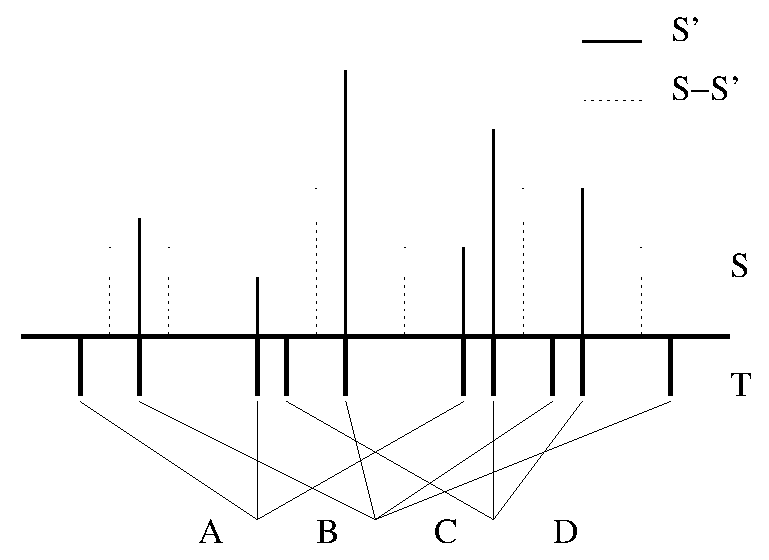
\includegraphics[width=0.6\textwidth]{./img/spectrum_sigma_theta.eps}
\caption{\label{fig:spec-ex}
Representation of a hypothetical target spectrum $\Sigma$ of experimental peaks
$x_i=(\rho_i,I_i)$, matched by the theoretical peaks of $\Theta$,
produced by the amino acid sequence $P=ABCD$.
In the figure the subset $\Sigma'$ represent the experimental peaks matched by
at least one theoretical peak.}
\end{center}
\end{figure}

We have seen in table \ref{tab:list} in section \ref{sec:shannon} of chapter
\ref{chap:db}, that CID fragmentation yields several different ion types:
$a,b,c,x,y,z$, with different charges and possible neutral losses. 
However, it 
is not expected, a priori,  that the full list of ions is produced at every fragmentation 
site, since the number and intensities of the
produced peaks greatly depend on different factors, including the three dimensional structure of
the peptide during fragmentation, or the instrument type.
For this reason, let's define  $\Theta_\nu$, a subset of $\mathcal T_\nu$,  as
the ions that have actually been generated from fragmentation at $\nu$, during
the experiment.
The corresponding collection of ions generated at any position will be
$\Theta=\{\Theta_{\nu_k}, k=1,\dots,L-1\}$. 
Any ion in $\Theta$ is characterized by a  mass-over-charge ratio $\rho$,
representing a theoretical peak position; to test the correspondence between
experimental  ($\Sigma$) and theoretical ($\Theta$)
spectra, we define the \emph{image} of a peak $s_i(\nu_k)$ in the spectrum $\Sigma$ as:
\begin{equation}
\mathcal I(s_i(\nu_k)):
\left\{
\pi\in\Sigma |
d\big(\rho(\pi),\rho(s_i(\nu_k))\big)<d_0
\right\}
\label{eq:map}
\end{equation}
where $d$ is the distance between the positions ot the experimental and
theoretical peaks (we will simply choose  $d(\rho_1,\rho_2)=\vert \rho_1-\rho_2\
vert $),  and $d_0$ is a cutoff distance, that we will take to depend linearly
on the position  of the product ion $\rho$, since it is  a reasonable hypothesis
that the errors on a spectral measure
are also proportional to the mass. %.value of the product ion $\rho$.
With this assumption we take %introduce a distance cutoff dependant on the peak's mass-to-charge value: 
$d_0= min(\gamma_1,\rho(s_i(\nu_k)) \gamma_2)$,
where the parameters $\gamma_1$ and $\gamma_2$ are empirically chosen with the
values $\gamma_1=2.0$ and $\gamma_2=0.0006$.

 Notice that in Eq.~\ref{eq:map} the image of a fragment could be represented by
several peaks, or also be the null set $\emptyset$. We then define
% The previous assumptions, and the definition of matching peaks defined on
% \ref{eq:map}, lead to the definition of a subset of $\Sigma$ and $\Theta$ with
% matched and matching peaks. 
%We define then
the subset $\Theta'_\nu$ of $\Theta_\nu$,  composed of  the
theoretical ions  produced in the fragmentation at $\nu$, that effectively match
at least one peak from the real
spectrum $\Sigma$:
\begin{equation}
\Theta'_\nu=%\Theta'_\nu(\Sigma,\Theta_\nu)=
\left\{
s_i(\nu)\in\Theta_\nu \vert
\mathcal I(s_i (\nu)) \neq \emptyset
\right\}
\end{equation}
Analogously,  the subset of the experimental spectrum $\Sigma$ of peaks that are the image of 
%matched by 
the theoretical peaks of $\Theta'_\nu$ can be defined as:
\begin{equation}
\Sigma'_\nu=%\Sigma'_\nu(\Sigma,\Theta'_\nu)=
\left\{
\mathcal I(s_i(\nu)) \vert s_i(\nu)\in\Theta'_\nu \right\}
\end{equation}
The corresponding global sets: $\Theta'=\{\Theta'_{\nu_k}, k=1,\dots,L-1\}$ and
$\Sigma'=\{\Sigma'_{\nu_k}, k=1,\dots,L-1\}$ are defined as before.

We observe that  the experimental peaks in  $\Sigma'$ need not necessarily be
the real image of the corresponding theoretical fragment:
% Theoretical peaks expected from the fragmentation at the peptide bond in $\nu$
% and that effectively match a experimental peak (those that compose
% $\Theta'_\nu$) can be interpreted in two different ways: the experimental peak
% is indeed the expression of the fragmentation event and in particular of the ion
% species $s_\nu$; on the other hand, 
indeed, if several experimental peaks can match the same fragment ion at $\nu$,
at most one of them will be  the real image of the fragment, the rest being a
product of noise. However,
there is also  the possibility that the ion $s_i$ was not recorded for some
reason, and all the experimental
matching  peaks  are a product of noise. Finally,   both $P$ and the noise could
contribute to the observed intensity of the same peak.
To deal with this possibilities, we introduce the concept of \emph{expressed peak}, referring to 
%We call \emph{expressed peaks} 
those ions of $\Theta'_\nu$ that effectively
produced a peak in $\Sigma'_\nu$:
\begin{equation}
\mathcal E(s_i(\nu))=
\left\{
\begin{aligned}
&1&&\textrm{if}\ \exists\ \pi\in\Sigma'_\nu|s_i(\nu)\to\pi\\
&0&&\textrm{otherwise}
\end{aligned}
\right.
\end{equation}
%With this interpretation in mind one can then 
and we define last two subsets of
$\Sigma$ and $\Theta$ with the expressed ions and the corresponding experimental
peaks:  (even if we might not be able to identify them among the others):
\begin{align}
\Theta''_\nu %=\Theta''_\nu(\Sigma,\Theta'_\nu)
&=
\left\{
s_i(\nu) \in \Theta'_\nu | \mathcal E(s_i(\nu))=1\right\}\\
\Sigma''_\nu&=
\left\{
\mathcal I(s_i(\nu)) | s_i(\nu)\in\Theta''_\nu
\right\}
\end{align}


% Can occur that a theoretical ion matches two or more real peaks, in this case it is more likely
% that only one represents the ion expression while the others are just noise.
% We can not distinguish \emph{a priori} which of them represents a fragment and
% which represents instrument noise (we will later introduce a \emph{a posteriori}
% selection rule).

%\begin{figure}
%\centering
%\begin{pspicture}(0,0)(8,-6)
%%\psgrid(0,0)(0,0)(8,-10)
%\rput(4,-1){\rnode{T}{\psframebox{$\Theta\equiv P$}}}
%\rput(4,-2.5){\rnode{T1}{\psframebox{$\Theta'$}}}
%\rput(3,-2.5){\rnode{T11}{\psframebox{$\Theta'$}}}
%\rput(2,-2.5){\rnode{T12}{\psframebox{$\Theta'$}}}
%\rput(1,-2.5){\rnode{T13}{\psframebox{\dots}}}
%\rput(4,-5.5){\rnode{T2}{\psframebox{$\Theta''$}}}
%\rput(6,-1){\ovalnode{S}{$\Sigma$}}
%\rput(6,-4){\ovalnode{S1}{$\Sigma'$}}
%\rput(6,-5.5){\ovalnode{S2}{$\Sigma''$}}
%\ncline[nodesepB=1pt]{->}{T}{T1}
%\ncline[linestyle=dashed,nodesepB=1pt]{->}{T}{T11}
%\ncline[linestyle=dashed,nodesepB=1pt]{->}{T}{T12}
%\ncline[linestyle=dashed,nodesepB=1pt]{->}{T}{T13}
%\ncline[nodesepB=1pt]{->}{T1}{S1}
%\ncline[nodesepB=1pt]{->}{S}{S1}
%\ncline[nodesepB=1pt]{->}{S1}{S2}
%\ncline[nodesepB=1pt]{->}{S1}{T2}
%\ncline[nodesepB=1pt]{->}{T1}{T2}
%\end{pspicture}
%\caption{\label{fig:sets}caption}
%\end{figure}

To avoid to deal with mixed situations as those described above, we can assume that:
\begin{hypothesis}
If $\pi$ is a experimental peak of $\Sigma''$, we assume that it is entirely due
to the corresponding species $s_i\in\Theta''$
\end{hypothesis}
Also, we assume that:
\begin{hypothesis}
The chances of multiple matches to the same experimental peak $\pi$ by different
fragment ions are negligible.
\end{hypothesis}
The above defined sets imply that all the peaks in $\Sigma \setminus \Sigma''$
are a product of noise, and that all the fragment ions in 
$\Theta'\setminus \Theta''$ have not produced any peak in the spectrum.
% 
% Some further remarks on those sets. The set of
% matched peaks $\Sigma'_\nu$ is completely defined from the definition of the
% spectrum $\Sigma$ and the matchable peaks $\Theta'\nu$. 
% This does not represent a
% one-to-one correspondence between $\Theta'_\nu$ and $\Sigma'_\nu$ as there can be some
% matchable peaks that actually do not match any experimental peak
% $\Theta'_\nu\setminus\Theta''\nu$; moreover some matchable fragments can actually match
% more than only one real peak if they fall \emph{near} the theoretical expected
% $\rho$.
% 
% We face also to some rare event like a peak from the spectrum is mathched by
% more then one expected ion from the peptide.
% We consider as negligeble this event:

%As reported previously, from the latter we will select one and only one
%experimental peak that will be the product of matchable theoretical ion.

\section{Protein sequencing as a an inference problem}

%\section{An Insight into the Probability}

 Let us consider the problem of spectra interpretation as a Bayesian inference
problem. We have seen that three different elements are involved in the MS/MS
experiment, 
$P$, $\Sigma$ and $R^\Sigma$, that can be considered as random variables,
extracted from different distributions.
Their joint probability  $p(P,R^\Sigma, \Sigma)$ can be
written as: %ans hypothesis \ref{hyp:p-r} as:
\begin{align}
p(P,R^\Sigma,\Sigma)&=p(\Sigma \vert P,R^\Sigma)p(P, R^\Sigma)\\
&= p(P \vert \Sigma, R^\Sigma)p(\Sigma, R^\Sigma)
\label{eq:p1}
\end{align}
introducing the conditional probabilities $p(\Sigma \vert P,R^\Sigma)$ of
observing the spectrum $\Sigma$ given the parent sequence $P$ and the source
$R^\Sigma$, and $p(P \vert \Sigma,R^\Sigma)$ of the parent sequence $P$ given
the observed spectrum $\Sigma$  and the noise  $R^\Sigma$.

We assume that the events generating spectrum noise are completely independent from
the precursor ion  and the fragmentation process that produce the true peaks:
\begin{hypothesis}
$R^\Sigma$ is uncorrelated from the peptide sequence $P$:
$p(P,R^\Sigma)=p(P)p(R^\Sigma)$.
\label{hyp:p-r}
\end{hypothesis}
% We consider then the join probability $p(P,R^\Sigma, \Sigma)$ which can be
% written using Bayesian rules ans hypothesis \ref{hyp:p-r} as:
% \begin{equation}
% p(P,R^\Sigma,\Sigma)=p(\Sigma|P,R^\Sigma)p(P)p(R^\Sigma)
% \label{eq:p1}
% \end{equation}

We also consider the noise distribution to be the same for every spectra, and to
be independent from the \emph{a-priori} distribution of the spectra:
\begin{hypothesis}
$R^\Sigma$ is independent from the target spectrum
$\Sigma$: $R^\Sigma\approx R\quad \forall \Sigma$, and
$p(R^\Sigma,\Sigma)\approx p(R)p(\Sigma)$.
\label{hyp:r-s}
\end{hypothesis}

Our goal is to estimate the posterior probability $p(P\vert R,\Sigma)$ that the
peptide $P$ is the precursor ion, given the experimental spectrum $\Sigma$ and
noise distribution $R$. However, we observe that in any \emph{de-novo} framework
the actual sequence $P$ cannot be resolved by the experiment, because of the
possible  mass degeneracies as between Isoleucine and Leucine: for instance, in
our modelling scheme, peptides differing by these residues at the same position
would correspond to the same configuration of our one-dimensional system,
characterized by the same set of fragmentation sites $\mathcal F(P)$ and
corresponding theoretical ions
we are interested in determining $\mathcal T(P)$ from the MS/MS data, since
$\mathcal T(P)$.
% 
% Moreover, we note that the correspondence between $P$ and the set of corresponding theoretical ions $\mathcal T(P)$
% is not one-to-one, at difference from the relation between the theoretical ions  $\mathcal
% T(P)$ and the fragmentation sites %peptide bond sites 
% $\mathcal F(P)$.
% Indeed,  the same set $\mathcal T(P)$ can correspond to several precursor sequences $P$, due to the degeneracy between 
% % the case, for example, of sequences containing 
% Leucine and Isoleucine. 
On the other hand, once given $P$,  the sets $\mathcal F(P)$ and $\mathcal T(P)$
are completely determined.
Therefore we can write, for any random variable $Y$:
\begin{equation}
p(P \vert Y)\equiv p(P,\mathcal T(P)\vert Y)=p(P|\mathcal T(P), Y)p(\mathcal T(P)\vert Y)
\label{eq:p-t}
\end{equation} 

This is true in particular for 
\begin{equation}
 p(P \vert R,\Sigma)=p(P \vert \mathcal T(P)) p(\mathcal T(P)\vert R,\Sigma)\,.
\label{eq:goal}
\end{equation}
where we have used the fact that  $ p(P \vert \mathcal T(P), \Sigma, R)=p(P
\vert \mathcal T(P))$, since no extra information about $P$, with respect to the
one contained in $\mathcal T(P)$, is carried by $\Sigma$ or $R$.
So, Equation \ref{eq:p1}, using Equations \ref{eq:p-t}, \ref{eq:goal} and hypothesis
\ref{hyp:r-s} can be rewritten in the following way:

\begin{align}
p(P,R,\Sigma)&=p(\Sigma \vert P,R) p(P|\mathcal T(P)) p(\mathcal T(P)) p( R)\\
&= p(P \vert \mathcal T(P)) p( \mathcal T(P) \vert \Sigma, R)  p(\Sigma) p(R)
\label{eq:p2}
\end{align}
% 
% \begin{equation}
% p(P,R,\Sigma)=p(P|\mathcal T(P),R,\Sigma)p(\mathcal T(P)|R,\Sigma)p(R)p(\Sigma)
% \label{eq:p2}
% \end{equation}
% that
% in the sequence $P$ itself because degeneracies as Leu-Ile cannot be resolved in
% the mass spectrometry framework.

Thus, %using equations \ref{eq:p1} and 
from Eq. \ref{eq:p2} one can finally write:
\begin{equation}
p(\mathcal T(P)\vert R ,\Sigma)=
p(\Sigma\vert P,R)
\frac{p(\mathcal T(P))}{p(\Sigma)}
\label{eq:start}
\end{equation}
which expresses Bayes theorem, and will be our starting point in the following. 
%of our implementation, searching 
Interpreting the spectrum will be equivalent to finding the peptide
sequence $P'$ that maximize probability \ref{eq:start}:
\begin{equation}
P'=\underset{P}{\text{argmax}}[p(\mathcal T(P)\vert R,\Sigma)]=
\underset{P}{\text{argmax}}[p(\Sigma|P,R)p(\mathcal T(P))]\,\,,
\label{eq:bestP}
\end{equation}
where we neglect the denominator, which is the same in all the maximization
process. Such $P'$ is the best prediction we can give of the true precursor ion
$P^*$.

In the above expression, $p(\mathcal T(P))$ is unknown, but some reasonable
assumptions can be made on it, basing, for instance, on the amino acid
frequencies, or on some other \emph{a-priori} information on the system under study.
The key point is, however, how to estimate the probability $p(\Sigma \vert P,
R)$ that, given a sequence $P$, (represented by its set of theoretical fragments
$\mathcal T(P)$ encoded in the state variables of our model) and a source of
statistical noise $R$, we will observe the experimental spectrum $\Sigma$.

If the physics of the fragmentation process in CID was well understood, along
with the distribution of contaminants and other factors responsible for the
noise peaks of a spectrum, we could calculate,  for any individual parent
peptide molecule, the probability of fragmentation $p^{\texttt{true}}(s_i|P)$
at any site , involving the generation of any ion species $s_i$. Such
probability, together with the corresponding one, $p(\rho|R)$, that the noise
$R$ is contributing at position $\rho$,  would allow to calculate the true
$p(\Sigma \vert P, R)$ for any $P$
%Such probability would be directly proportional to the corresponding peak intensities, so that,
% given a parent peptide and a model for the contaminants intervening in its
% measure, a theoretical spectrum could be associated to any experimental setup
% and precursor peptide.
Identification would then proceed by comparing the experimental spectrum with
the theoretical ones associated to all the possible parent peptides, and
choosing the peptide whose theoretical spectrum is most similar to the
experimental one (using some suitable measure of similarity, as for instance
Kullback-Leibler distance). In this approach, the theoretical spectra would be
calculated from first principle, with a ``true'' Hamiltonian function, and the
information from the experimental spectrum would be used a posteriori, in the
comparison of the average intensities.

The lack of a suitable \emph{ab-initio} Hamiltonian to describe the
fragmentation process prompts for a different approach, where information
proceeding from the experimental spectrum itself, or by the typical peak
distributions in a database of spectra, is used to derive an ad-hoc energy
function, so that the experimental spectrum acts as an ``external field''
biasing the system towards the most-likely parent peptide sequence.

We will use the latter approach here, which is common to all \emph{de-novo}
methods. We will also adopt a different view on the MS/MS spectra generation:
instead of considering a spectra  as the outcome  from an ensemble of molecules,
and of describing the fundamental process as the fragmentation of one single
molecule into two pieces during CID,  we will consider the whole spectrum as the
overlap between the signal from a noise source and from the fragmentation in
multiple sites of a unique parent sequence, both of them generating peaks ``as a
whole'', with a characteristic position and intensity $(\rho,I)$.
In other words, due to our ignorance of the true energy function underlying the
spectra generation, we move away from the (physically correct) view of a MS
spectrum as the overlap between the weak signals of an ensemble of individual
products ions, and adopt a more bioinformatics-oriented view of a spectrum
generated by a unique entity, yielding several ion products at each
fragmentation site $\nu$, that are rewarded or penalized according to an
external empirical potential, based on our results of the previous chapter, on
the distribution of probability of the peaks in the $(\rho,I)$ plane. This
approach allows us to reward the presence in the spectrum of several ion species
representing fragmentations at the same position along the sequence (e.g,
detection of $y$ $b$, etc. ions originating from fragmentations at the same
position $\nu$).

To define the energy function, we need to develop Eq.~\ref{eq:start} in finer detail.



Let us call $\mathcal A^\Sigma(P)$ an assignment of the sequence $P$ on the
spectrum $\Sigma$, specifying which theoretical ions $\Theta$ were actually
produced, which of them $\Theta''$  were  detected, and which were the
corresponding peaks $\Sigma''$ in the spectrum:
\begin{align}
\mathcal A^\Sigma(P)=\{\Theta,\Theta'',\Sigma''\}&\equiv
\{\Theta,\Theta'',\Sigma'';\Theta\setminus\Theta''\}
\label{eq:assignment}
% \\
% \intertext{where}
% \Theta''&=\bigcup_{\nu\in\mathcal F(P)} \Theta''_\nu\\
% \Sigma''&=\bigcup_{\nu\in\mathcal F(P)} \Sigma''_\nu
\end{align}
The last expression underlines that, given $\Theta$  and $\Theta''$, the set of
fragmentations that have not produced a peak in the spectrum is also completely
determined as $\Theta\setminus\Theta''$.



The probability $p(\Sigma|P,R)$ can be written as the sum over the different
ways that spectrum peaks can be assigned to the sequence $P$:
%is this case calculated in term of assignment
% as in \ref{eq:assignment} that interprets in different ways the association of
% theoretical peaks calculated from the proposed sequence $P$ and the spectrum
% peaks.
% The equation \ref{eq:start} takes the form:
\begin{align}
p(\Sigma|P,R)&=
\sum_{\mathcal A^\Sigma(P)}
p(\Sigma,\mathcal A^\Sigma(P)|P,R)=\\
&=
\sum_{\mathcal A^\Sigma(P)}
p(\Sigma|\mathcal A^\Sigma(P),P,R)
p(\mathcal A^\Sigma(P)|P,R)
\label{eq:assign_sum}
\end{align}
where the sum over $\mathcal A^\Sigma(P)$ involves all possible choices of  $\Theta \subset \mathcal
T$, $\Theta''\subset \Theta'$ and $\Sigma''\subset \Sigma'$.
As we mentioned, 
this implies that there may be some theoretical ions $s\in\Theta'\setminus\Theta''$
that are considered to have escaped detection, and %, even if they could be matching %, while they are matching 
if any peaks  of the spectrum could match them, the latter are considered as noise.
Moreover, this also implies that when  a single theoretical ion $s$ can match more
than  one spectrum peak, the sum also involves all the way the ``true'' image of $s$ can be chosen in $\Sigma'$.
To simplify the approach we introduce two hypotheses:
\begin{hypothesis}
If an ion species $s\in\Theta'$ can match an experimental peak $\pi\in\Sigma$,
then the peak should be interpreted as the image of $s$.
\label{hyp:theta2}
\end{hypothesis}
\begin{hypothesis}
If an ion species $s\in\Theta'$ matches more than one experimental peak in $\Sigma$,
then the true image of $s$ will be the peak $\pi$ that maximize the probability
(at fixed $\Theta$ and $\Theta''$).
\label{hyp:sigma2}
\end{hypothesis}
On the basis of the hypothesis \ref{hyp:theta2}, we can say that
$\Theta''\equiv\Theta'\subseteq\Theta$. From the hypothesis \ref{hyp:sigma2} it
follows that the peak set $\Sigma''$ is completely determined by the definition
of $\Sigma,\Theta$ and $\Theta''$.
Following previous hypothesis (\ref{hyp:theta2} and \ref{hyp:sigma2}), 
the sets $\Theta''$ and $\Sigma''$ in the assignment $\mathcal A^\Sigma(P)$
remains completely determined  once defined the set  $\Theta$, so that the sum
in Eq.~\ref{eq:assign_sum} is simplified:
\ref{eq:assign_sum} change to:
\begin{equation}
p(\Sigma|P,R)=
\sum_{\Theta\in\mathcal T(P)}
p(\Sigma|\mathcal A^\Sigma(P),P,R)p(\mathcal A^\Sigma(P)|P,R)
\label{eq:sigma_sum}
\end{equation}
The probability $p(\Sigma|\mathcal A^\Sigma(P),P,R)$, given the assignment
$\Theta,\Theta''$ and $\Sigma''$, corresponds to the probability that
the remaining unassigned peaks in $\Sigma\setminus\Sigma''$ are due
to noise. Under the hypothesis:
\begin{hypothesis}
Peaks due to noise are independent random events;
\label{hyp:indipR}
\end{hypothesis}
such probability can be factorized as:
\begin{equation}
p(\Sigma|\mathcal A^\Sigma(P),P,R)=
p(R\to\Sigma\setminus\Sigma''|R)=
\prod_{\pi\in\Sigma\setminus\Sigma''}
p(R\to\pi|R)
\end{equation}
The probability of the assignment
$\mathcal A^\Sigma(P)$ is independent from the noise events and thus $p(\mathcal
A^\Sigma (P)|P,R)\equiv p(\mathcal A^\Sigma(P)|P)$.

It would be desirable to propose a factorized form also for the latter probability. 
However, the events that underlie the assignment of the theoretical peaks in
$\Theta''$ to the experimental peaks of $\Sigma''$ are correlated and cannot be
factorized on each $\nu$: for instance the probability of having a peak
corresponding to the ion $s_i(\nu_1)$ and that of a peak from ion $s'_i(\nu_2)$
are not independent. However, we can restrict our attention only to the
fragmentation sites of $P$, and not to all $\nu$, and assume that in this case:
\begin{hypothesis}
Probabilities of different fragmentation sites are independent and can be
factorized on $\nu\in\mathcal F(P)$.
\end{hypothesis}
\begin{hypothesis}
Within a given choice of ion species $\Theta_\nu\subseteq\mathcal T_\nu(P)$
produced in $\nu$, the probabilities are independents and can be factorized on
$s_i(\nu)$.
\end{hypothesis}

With this hypotheses we can rewrite Equation \ref{eq:sigma_sum} as:
\begin{multline}
p(\Sigma|P,R)=
\sum_{\Theta\subseteq\mathcal T(P)}
\left[
\prod_{\pi\in\Sigma\setminus\Sigma''}
p(R\to\pi|R)
\right]\times\\
\times\prod_{\nu\in\mathcal F(P)}
\left\{
\left[
\prod_{s_i(\nu)\in\Theta'_\nu}
p^\text{loc}(s_i\to\Sigma''(s_i),s_i\in\Theta_\nu,s_i\in\Theta'_\nu|P)
\right]
\right.\\
\left.
\left[
\prod_{t_\nu\in\Theta\setminus\Theta'_\nu}
p^\text{loc}(t_\nu\to\emptyset,t_\nu\in\Theta_\nu,t_\nu\in\Theta\setminus\Theta'_\nu|P)
\right]
\right\}
\end{multline}
where $p^\text{loc}(*)$ indicates that the probability is normalized in a small
neighborhood of the theoretical position $\rho(s_i(\nu))$, according
to the fact that, once determined the precursor peptide $P$, the fragmentation
sites $\nu\in\mathcal F(P)$ and then the expected ions $s_i$ are completely
fixed. 

We can then write:
\begin{multline}
p(\Sigma|P,R)=
\Bigg\{\prod_{\nu\in\mathcal F(P)}
\Bigg[\sum_{\Theta_\nu\in\mathcal T_\nu(P)}
\prod_{s_i(\nu)\in\Theta_\nu}\Big(
(1-\delta_{\mathcal I(s_i),\emptyset})w^M(s_i,\mathcal I(s_i))+\\
+\delta_{\mathcal I(s_i),\emptyset}w^{\bar M}(s_i)
\Big)\Bigg]\Bigg\}\times
p(R\to\Sigma)
\label{eq:psigma}
\end{multline}
where
\begin{align}
w^M(s_i,\mathcal I(s_i))&=
\frac{p^\text{loc}(s_i\to\Sigma''(s_i),s_i\in\Theta_\nu,s_i\in\Theta'_\nu|P)}
{p(R\to\Sigma''(s_i)|R)}\\
w^{\overline M}(s_i)&=
p^\text{loc}(s_i\to\emptyset,s_i\in\Theta_\nu,s_i\in\Theta_\nu\setminus\Theta'_\nu|P)\\
p(R\to\Sigma)&=
\prod_{\pi\in\Sigma} p(R\to\pi|R)
\label{eq:wM}
\end{align}
we introduce the dynamical variable $\xi_\nu^{s_i}$ that indicate if there
fragmentation of the peptide in $\nu$ produced the ion $s_i$ or not:
\begin{equation}
\xi_\nu^{s_i}=\left\{
\begin{aligned}
&1 && \text{if\ } s_i\in\Theta_\nu\\
&0 && \text{if\ } s_i\in\mathcal T_\nu\setminus\Theta_\nu
\end{aligned}
\right.
\end{equation}
that let us write equation \ref{eq:psigma} as:
\begin{multline}
p(\Sigma|P,R)=
p(R\to\Sigma)\times
\Bigg\{\prod_{\nu\in\mathcal F(P)}
\prod_{s_i\in\mathcal T_\nu(P)}\Bigg[
\sum_{\xi_\nu^{s_i}=0,1} \Bigg( 
\delta_{\xi_\nu^{s_i},0}+ \\
+\delta_{\xi_\nu{s_i},1}\Big(
(1-\delta_{\mathcal I(s_i),\emptyset})w^M(s_i,\mathcal I(s_i))
+\delta_{\mathcal I(s_i),\emptyset}w^{\bar M}(s_i)
\Big)
\Bigg)
\Bigg]\Bigg\}
\end{multline}

Finally, we go back to Eq.~\ref{eq:start} and we make another assumption on the
\emph{a-priori} probability of the theoretical fragments:
\begin{hypothesis}
The probability $p(\mathcal T(P))$ of the set of theoretical ions from peptide
$P$ can be factorized on individual ions, as independent statistical events; the
\emph{a-priori} probability of any fragment $s_i$  is independent from its type:
\end{hypothesis}
Hence,
\begin{equation}
p(\mathcal T(P))=\prod_{\nu\in\mathcal F(P)}
\prod_{s_i\in\mathcal T_\nu(P)} p_\text{ion}
\end{equation}
where $p_\text{ion}$ is a constant for all fragmentation sites $\nu$ and species
$s_i$.

In the end, our proposal for the posteriori probability  of observing $P$ as the
parent peptide, given the experimental spectrum $\Sigma$ and a model $R$ for the
noise, is given by Eq.~\ref{eq:goal} together  with
Eq.~\ref{eq:bestP} and:
\begin{multline}
p(\mathcal T(P)\vert \Sigma, R) \propto
p(R\to\Sigma)\times
\Bigg\{\prod_{\nu\in\mathcal F(P)}
\prod_{s_i\in\mathcal T_\nu(P)}
p_{\text{ion}}
\Bigg[
\sum_{\xi_\nu^{s_i}=0,1} \Bigg( 
\delta_{\xi_\nu^{s_i},0} +\\
+\delta_{\xi_\nu^{s_i},1}\Big(
(1-\delta_{\mathcal I(s_i),\emptyset})w^M(s_i,\mathcal I(s_i))
+\delta_{\mathcal I(s_i),\emptyset}w^{\bar M}(s_i)
\Big)\Bigg)
\Bigg]\Bigg\}
\label{eq:finalp}
\end{multline}


%------------------------------------------------------------------

\section{An empirical Energy Function}
\label{potential}
Equation \ref{eq:finalp} provides us with a recipe to evaluate the fitness of
any sequence $P$ to match the spectrum $\Sigma$, as a product over all the
fragmentation sites $\nu \in \mathcal F(P)$ of $P$, and over all the possible
theoretical fragment ions that could in principle be generated by sequence $P$,
of the probability to generate any fragment, times a term accounting for all the
possible patterns in which the ions  $s_i$ can be  actually generated, and, if
they are, weighting the probability to have generated a peak in the spectrum
($w^M$), or to have produced no peak ($w^{\bar M}$).
The above expression is further multiplied by the probability $p(R\to\Sigma)$
that the whole spectrum is generated by the noise. The latter term is
independent from the parent sequence, so that we can ignore it in the following,
and keep the rest of the expression as a guide to introduce an ad-hoc
Hamiltonian for our model, by writing:
\begin{equation}
p(\mathcal T(P)\vert \Sigma, R) \propto
\Bigg\{\prod_{\nu\in\mathcal F(P)}
\Bigg[
\prod_{s_i\in\mathcal T_\nu(P)}
\left(
\sum_{\xi_\nu^{s_i}=0,1} e^{-\beta H(\nu,s_i,\xi_\nu^{s_i})}
\right)
\Bigg]\Bigg\} \,\,,
\end{equation}
where $\beta$ is a fictitious inverse temperature, and  we have introduced:

\begin{multline}
H(\nu,s_i,\xi_\nu^{s_i})=\mu-\delta_{\xi_\nu^{s_i},1} 
\Big(
(1-\delta_{\mathcal I(s_i),\emptyset}) \log (w^M(s_i,\mathcal I(s_i))+\\
+\delta_{\mathcal I(s_i),\emptyset} \log (w^{\bar M}(s_i))
\Big)\,,
\label{eq:Ham}
\end{multline}
defining the chemical potential as $\mu=-\log p_{\text{ion}}$.

This corresponds to defining the energy function in terms of the probabilities
contained in the expressions of $w^M$ and $w^{\bar M}$ in Eq.~\ref{eq:wM}, that
are, however, unknown. We propose an empirical estimate for such quantities
resorting to the results of chapter \ref{chap:db}, on the
phenomenological distributions obtained by the analysis of a large  database of
spectra with the associated predicted precursor ion.

Namely, in order to define the probability of matching a real peak
$p^\text{loc}(s_i\to\Sigma''(s_i),s_i\in\Theta_\nu,s_i\in\Theta'_\nu|P)$
and the probability of a theoretical ion to not match any experimental peak
$p^\text{loc}(s_i\to\emptyset,s_i\in\Theta_\nu,s_i\in\Theta\setminus\Theta'_\nu|P)$,
we express them in term of database frequencies.
The former represents the probability that, given the fragmentation site 
$\nu\in\mathcal F(P)$, the dissociation event produced the species $s_i$ and
this was detected as a peak in the final spectrum.
In a similar way, the latter represents the probability that, given
$\nu\in\mathcal F(P)$, the species $s_i$ was produced, but for some reason it
did not yield any peak in the experimental spectrum.
We express these probabilities as:

\begin{align}
p^\text{loc}(s_i\to\Sigma''(s_i),s_i\in\Theta_\nu,s_i\in\Theta'_\nu|P)
&=
\frac{N(s_i,x(\Sigma''(s_i)))}
{\displaystyle
\sum_{t\in\mathcal T_\nu(P)}N^T(t,\mathcal J_\delta(\rho(t)))}
\\
p^\text{loc}(s_i\to\emptyset,s_i\in\Theta_\nu,s_i\in\Theta\setminus\Theta'_\nu|P)
&=
\frac{N(\bar s_i,\mathcal J_\delta(\rho(s_i)))}
{\displaystyle
\sum_{t\in\mathcal T_\nu(P)}N^T(t,\mathcal J_\delta(\rho(t)))}\\
p(R\to\pi|R)
&=
\frac{N(R,x(\pi))}{N(R)}
\end{align}
where $x(\pi)$ represents the cell in which the peak $\pi$ fall, in the cell the
distribution of peaks is taken as constant; $\mathcal J_\delta(\rho)$ represents
the interval $[\rho-\delta,\rho+\delta]$ and considers all peak intensity
values.
$N(x,y)$ represents the frequency of peaks matched as $x$ inside the interval
$y\equiv y_\rho\times y_I$ and $N(\bar x,y_\rho)$ the number of absent $x$ type
ions in the interval $y_\rho$, while $N^T(x,y_\rho)$ represent the expected number of peaks $x$ in the
$y_\rho$ interval of the $\rho$ axis accounting for both matched and absent peaks:
$N^T(x,y_\rho)= N(\bar x,y_\rho)+\sum_I N(x,y_\rho\times y_I)$.

 Finally, we note that also the value of the
\emph{chemical potential} $\mu$ defined above is unknown. 
We observe that its practical role is to penalize the system against matching
the experimental spectrum with too many fragment ions, i.e., using sequences
with the highest allowed  number of residues (and fragmentation sites),
polarizing the result towards the lightest residues, ending up in an excess
of Glycines.
For this reason, we fix it 
\emph{a posteriori}, optimizing the agreement between the predicted peptide and
the ``true'' parent, as predicted  by SEQUEST, for the spectra in the learning
database.


\chapter{Results and Discussion}
\label{chap:msms-results}

%The algorithm described in the previous chapters has been implemented in a
%in-house software called ``\ournovo'' and written in C++ language.
%It expects as input a SEQUEST-type spectrum (*.dta) which in composed by an
%header row with the precursor ion mass ($m(MH^+)$) and charge ($Q$).
%The following rows of the input spectrum file
% are composed by the peaks centroids and their intensities.
%The resulting software gives the possibility to provide a test
%sequence input, as a comparing term for the algorithm prediction, and a precursor mass, to override
%the value contained in the spectrum file.
%%to force the model to accept this value.

\section{Testing Methods}

To test the algorithm described in the previous chapters, we have applied it to a
test set kindly provided to us by \citet{fischer2005novohmm}, and originally
selected by \citet{pepnovo-analchem-2005}, of experimental mass spectra.
This test set is composed by 280 spectra of double charged peptides up to 1400 Da. coming from
tryptic spectrometry
experiments, which is accompanied by a reliable sequence assignment by SEQUEST
algorithm\cite{pepnovo-analchem-2005}. 
It originates from a 18-protein mixture database by \citet{keller2002experimental}
and from the open proteomics database by \citet{prince-2004-prot-repository}.

We compare the outcoming model prediction to the provided sequence assignment
that we refer to as ``theoretical sequence''.
To provide a measure of the prediction correctness, we compute Precision (which represents the fraction
of correctly predicted fragmentation sites over the total number of proposed
fragmentation sites),
Recall (which represents correctly predicted sites over the total number of
fragmentation sites in the theoretical sequence) and their harmonic mean,
$F$-value, for both the profile and the best sequence
as described in Sec.~\ref{sec:teo-profile}.

%This measure is calculated in two slightly different ways, considering
%two different
%definitions of \emph{correct prediction} and \emph{proposed prediction}.
%In the first way the theoretical sequence is compared to the calculated
%fragmentation
%probability accounting for matching sites weighted by their probability.
%This, in some way, compare the whole thermodynamic system, in its equilibrium
%state, to the ``real'' peptide.
%In the second way we just compare the most probable sequence, calculated as described
%in Sec.~\ref{sec:msms-issues}, to the theoretical one, without considering the
%rest of the configurations. 
%See  Sec.~\ref{sec:teo-profile} for a detailed description.

We also probe our method on a prefiltered version of test spectra, removing the
peaks that are probably noise, as explained on the following.
We also study the effect of enforcing the current parent mass, when the method
fails to identify it: as can be seen from Fig. \ref{fig:test-dm}, there is a mismatch
$\Delta m\in [-0.5,1.2]$ between the mass corresponding to the theoretical
sequence and that recovered from the .dta input file, that induced a mass error
in 47 out of 280 spectra.

\begin{figure}
\begin{center}
\resizebox{0.6\textwidth}{!}{\sffamily% GNUPLOT: LaTeX picture with Postscript
\begingroup
  \makeatletter
  \providecommand\color[2][]{%
    \GenericError{(gnuplot) \space\space\space\@spaces}{%
      Package color not loaded in conjunction with
      terminal option `colourtext'%
    }{See the gnuplot documentation for explanation.%
    }{Either use 'blacktext' in gnuplot or load the package
      color.sty in LaTeX.}%
    \renewcommand\color[2][]{}%
  }%
  \providecommand\includegraphics[2][]{%
    \GenericError{(gnuplot) \space\space\space\@spaces}{%
      Package graphicx or graphics not loaded%
    }{See the gnuplot documentation for explanation.%
    }{The gnuplot epslatex terminal needs graphicx.sty or graphics.sty.}%
    \renewcommand\includegraphics[2][]{}%
  }%
  \providecommand\rotatebox[2]{#2}%
  \@ifundefined{ifGPcolor}{%
    \newif\ifGPcolor
    \GPcolorfalse
  }{}%
  \@ifundefined{ifGPblacktext}{%
    \newif\ifGPblacktext
    \GPblacktexttrue
  }{}%
  % define a \g@addto@macro without @ in the name:
  \let\gplgaddtomacro\g@addto@macro
  % define empty templates for all commands taking text:
  \gdef\gplbacktext{}%
  \gdef\gplfronttext{}%
  \makeatother
  \ifGPblacktext
    % no textcolor at all
    \def\colorrgb#1{}%
    \def\colorgray#1{}%
  \else
    % gray or color?
    \ifGPcolor
      \def\colorrgb#1{\color[rgb]{#1}}%
      \def\colorgray#1{\color[gray]{#1}}%
      \expandafter\def\csname LTw\endcsname{\color{white}}%
      \expandafter\def\csname LTb\endcsname{\color{black}}%
      \expandafter\def\csname LTa\endcsname{\color{black}}%
      \expandafter\def\csname LT0\endcsname{\color[rgb]{1,0,0}}%
      \expandafter\def\csname LT1\endcsname{\color[rgb]{0,1,0}}%
      \expandafter\def\csname LT2\endcsname{\color[rgb]{0,0,1}}%
      \expandafter\def\csname LT3\endcsname{\color[rgb]{1,0,1}}%
      \expandafter\def\csname LT4\endcsname{\color[rgb]{0,1,1}}%
      \expandafter\def\csname LT5\endcsname{\color[rgb]{1,1,0}}%
      \expandafter\def\csname LT6\endcsname{\color[rgb]{0,0,0}}%
      \expandafter\def\csname LT7\endcsname{\color[rgb]{1,0.3,0}}%
      \expandafter\def\csname LT8\endcsname{\color[rgb]{0.5,0.5,0.5}}%
    \else
      % gray
      \def\colorrgb#1{\color{black}}%
      \def\colorgray#1{\color[gray]{#1}}%
      \expandafter\def\csname LTw\endcsname{\color{white}}%
      \expandafter\def\csname LTb\endcsname{\color{black}}%
      \expandafter\def\csname LTa\endcsname{\color{black}}%
      \expandafter\def\csname LT0\endcsname{\color{black}}%
      \expandafter\def\csname LT1\endcsname{\color{black}}%
      \expandafter\def\csname LT2\endcsname{\color{black}}%
      \expandafter\def\csname LT3\endcsname{\color{black}}%
      \expandafter\def\csname LT4\endcsname{\color{black}}%
      \expandafter\def\csname LT5\endcsname{\color{black}}%
      \expandafter\def\csname LT6\endcsname{\color{black}}%
      \expandafter\def\csname LT7\endcsname{\color{black}}%
      \expandafter\def\csname LT8\endcsname{\color{black}}%
    \fi
  \fi
  \setlength{\unitlength}{0.0500bp}%
  \begin{picture}(7200.00,5040.00)%
    \gplgaddtomacro\gplbacktext{%
      \colorrgb{0.31,0.31,0.31}%
      \put(1032,768){\makebox(0,0)[r]{\strut{}-0.8}}%
      \colorrgb{0.31,0.31,0.31}%
      \put(1032,1130){\makebox(0,0)[r]{\strut{}-0.6}}%
      \colorrgb{0.31,0.31,0.31}%
      \put(1032,1492){\makebox(0,0)[r]{\strut{}-0.4}}%
      \colorrgb{0.31,0.31,0.31}%
      \put(1032,1854){\makebox(0,0)[r]{\strut{}-0.2}}%
      \colorrgb{0.31,0.31,0.31}%
      \put(1032,2216){\makebox(0,0)[r]{\strut{} 0}}%
      \colorrgb{0.31,0.31,0.31}%
      \put(1032,2578){\makebox(0,0)[r]{\strut{} 0.2}}%
      \colorrgb{0.31,0.31,0.31}%
      \put(1032,2941){\makebox(0,0)[r]{\strut{} 0.4}}%
      \colorrgb{0.31,0.31,0.31}%
      \put(1032,3303){\makebox(0,0)[r]{\strut{} 0.6}}%
      \colorrgb{0.31,0.31,0.31}%
      \put(1032,3665){\makebox(0,0)[r]{\strut{} 0.8}}%
      \colorrgb{0.31,0.31,0.31}%
      \put(1032,4027){\makebox(0,0)[r]{\strut{} 1}}%
      \colorrgb{0.31,0.31,0.31}%
      \put(1032,4389){\makebox(0,0)[r]{\strut{} 1.2}}%
      \colorrgb{0.31,0.31,0.31}%
      \put(1032,4751){\makebox(0,0)[r]{\strut{} 1.4}}%
      \colorrgb{0.31,0.31,0.31}%
      \put(1176,528){\makebox(0,0){\strut{} 0}}%
      \colorrgb{0.31,0.31,0.31}%
      \put(2108,528){\makebox(0,0){\strut{} 50}}%
      \colorrgb{0.31,0.31,0.31}%
      \put(3040,528){\makebox(0,0){\strut{} 100}}%
      \colorrgb{0.31,0.31,0.31}%
      \put(3972,528){\makebox(0,0){\strut{} 150}}%
      \colorrgb{0.31,0.31,0.31}%
      \put(4903,528){\makebox(0,0){\strut{} 200}}%
      \colorrgb{0.31,0.31,0.31}%
      \put(5835,528){\makebox(0,0){\strut{} 250}}%
      \colorrgb{0.31,0.31,0.31}%
      \put(6767,528){\makebox(0,0){\strut{} 300}}%
      \csname LTb\endcsname%
      \put(192,2759){\rotatebox{-270}{\makebox(0,0){\strut{}$\Delta m$}}}%
      \put(3971,168){\makebox(0,0){\strut{}spectra}}%
    }%
    \gplgaddtomacro\gplfronttext{%
    }%
    \gplbacktext
    \put(0,0){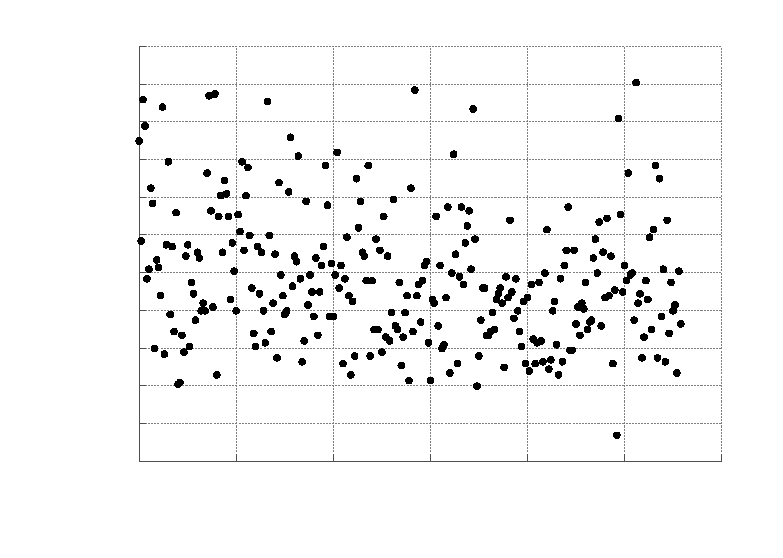
\includegraphics{img/msms/graph-deltamass-test}}%
    \gplfronttext
  \end{picture}%
\endgroup
}
\end{center}
\caption{\label{fig:test-dm} Distribution of the difference between the
precursor mass reported in the .dta file and the corresponding average mass calculated
from the true sequence in the test dataset ($\Delta m$).
The figure shows that the distribution of the $\Delta m$ exit the $[-0.5,0.5]$
range where an exact estimation of the precursor mass can be done by the model.}
\end{figure}


%%%%%%%%%%%%%%%%%%%%%%%%%%%%%%%%%%%%%%%%%%%%%%%%%%%%%%%%%%%%%%%%%%%%%%%%%%%%%%%
\section{Results}

In the following we present the results of the model implementation and
testing: we divide them into results at low temperature, in which the ``best
sequence'' is  %can be 
extracted and then compared with  predictions of other \emph{de-novo} algorithms,
and results concerning the temperature dependence of some thermodynamic quantities, that 
%into temperature varying results which 
are a feature of our model and
can give an insight  of %into the thermodynamics governing the system behaviour and let the user guess 
the quality of the prediction.

\subsection{The Low-Temperature Regime: Peptide Identification}

%% Choice of the number of species used
The sequencing algorithm resulting from the system described in the previous
chapters presents two parameters still to be determined.
The first parameter is the number of ion species to use to match the
experimental peaks at each fragmentation site, while 
the second parameter is the value of the chemical potential $\mu$ introduced in
Sec.\ref{potential}.
We fix the value of those parameters to the values that optimize the predictions
of the algorithm when applied to the learning database.
%The number of ions used in the spectrum matching is, then, three in the case of
%precursors singly or doubly charged and six in the case of triply charged
%precursors.
%The coupled value of $\mu$ is then 0.48, 0.56 and 0.28 in the respective cases.

%% Choice of the working temperature
We selected as working temperature $T=1$ which was the same temperature adopted
when learning the distributions from the database.
After some
preliminary tests, we saw indeed that 
this temperature was  a good choice, as it is low enough to assure that the
system is found basically %lives 
in the energy minimum, without freezing it in the ground state or
provoking numerical problems in the computation. %singularities.}

%% Choice of the chemical potential value
At this temperature we first tested the software against a selection of
spectra from the learning database (all spectra from the database of singly
charged precursors, 1000 spectra from the doubly charged and 160 from the triply
charged)
and determined the number of ions and value of the chemical potential $\mu$ that maximizes the $F$-value
separately for each charge value.
Here $\mu$ can be interpreted as a length limiting parameter as it will
discourage configurations of the system that match many peaks just by increasing
the sequence length, using smaller residues.
Such behaviour would increase the
Recall but decrease the value of the Precision.
The resulting values for the model parameters are: for singly charged
precursors, 3 ions and $\mu(Q=1)=0.48$, for doubly charged precursors 3 ions and
$\mu(Q=2)=0.56$, and for triply charged precursors 6 ions and $\mu(Q=3)=0.28$.

We compared the results of the algorithm with other popular \emph{de novo}
sequencing algorithms, such as NovoHMM, Lutefisk, Pepnovo, Pepnovo2011 described
in the Subsec.~\ref{subsec:others}. 
They were run
with the default parameters: NovoHMM was run with the non-grouping option,
PepNovo using the CID\_IT\_TRYP model.

For every algorithm we select the most probable sequence proposed and we compare
it with the theoretical sequence provided by SEQUEST. 
To perform a model comparison we compute TP, PP and RP as well as the $F$-value
for each of the peptides.
In Table \ref{tab:tab} we report the resulting values of precision, recall and
F-value.
If precision and recall values are very close to each other,
 then the model is not generating too many
fragmentation events in order to match at least a subset (rec.$>$prec.),
neither is producing a low number of events in order not to fail
(prec.$>$rec.).
It is fair to notice that Lutefisk and PepNovo algorithms do not predict the
entire sequence if they are not sure, so that their recall
will be lower than precision, in general.


\begin{table}
\centering
\begin{tabular}{l|cccc}
\hline \hline
Model & Precision & Recall & F'-value & Mass Mismatch\\
\hline
Lutefisk       & 0.664    & 0.717    & 0.688   &43\\
PepNovo	       & 0.665    & 0.691    & 0.676   &109\\
PepNovo 2011   & 0.589    & 0.652    & 0.616   &162\\
HMM            & 0.778    & 0.786    & 0.781   &12\\
\hline
%\ournovo       & 0.611    & 0.602    & 0.605   & 47\\
%\ournovo-pre   & 0.660    & 0.638    & 0.648   & 47\\ 
%\ournovo-M     & 0.696    & 0.690    & 0.692   &  0\\
%\ournovo-pre-M & 0.754    & 0.743    & 0.749   &  0\\
\ournovo       & 0.657	  & 0.642   & 0.649   & 47\\
\ournovo-pre   & 0.663	  & 0.647   & 0.654   & 47\\ 
\ournovo-M     & 0.747	  & 0.732   & 0.739   &  0\\
\ournovo-pre-M & 0.755	  & 0.740   & 0.747   &  0\\
\hline \hline
\end{tabular}
\caption{\label{tab:tab}
In this table we report the values of Precision, Recall and $F'$-value for
different algorithms. The last column shows the number of wrongly interpreted
precursor masses. True positives are calculated as the mean of true positive
accumulated masses from N-term and from C-term, as interpretation with wrong
precursor masses can bias the result. The runs of our model have been done with
the raw algorithm (\ournovo) or over a pre-filtered spectrum (-pre) or forcing
the algorithm to accept the true precursor mass (-$M$), calculated from the
theoretical sequence.}
\end{table}

Table \ref{tab:tab} shows that the model without modifications does not present 
high precision or recall values, although, in this particular set, results are
better than PepNovo2011, while the others algorithms perform slightly better.
It is interesting to notice that the better model in this test is the one that
shows a better recognition of the peptide mass.
We have introduced some modification in order to identify the model weaknesses.
We can force the algorithm to accept an external value of the parent mass ($M$),
to enforce that the mass of the ``true'' parent sequence is considered, when
such mass is not the same as that appearing in the spectrum file. We can  also
pre-process the spectrum in order to filter out some noise peaks (-pre).
The latter filtering is performed by selecting six peaks in each window of 100 Da and
discarding the others as noise as in \citet{Mo2007}.
From the results it is clear that a higher precision in the peptide mass detection
will increase noticeably the $F'$-value, while pre-processing the spectrum
to remove the noise peaks does not  improve notably the results.

%Despite the present 
%instrument sensibility, it is usual to find erroneous values of
%the precursor mass, sometimes accountable to human data mis-interpretation.
%As shown in Fig.~\ref{fig:mh-dist}, the difference between the mass provided by
%the instrument measure of the precursor peak and reported in the spectrum file
%and the mass expected for the amino acid content of the precursor has a wide
%distribution covering a range about 6 Da, in the learning databases.
%This confuses  the interpretation process.
%Notice that the actual distribution presents some peaks uniformly separated by 1
%Da that suggests a erroneous selection of the mono-isotopic precursor peak in
%the spectrometry procedure, see Subsec.~\ref{subsec:cid-spectrum} for a detailed
%description.
%\begin{figure}
%\centering
%\subfigure[tot]{
%\includegraphics[width=2cm,angle=-90]{./img/msms/MH-dist-small-tot.eps}}
%\subfigure[$Q=1$]{
%\includegraphics[width=2cm,angle=-90]{./img/msms/MH-dist-small-q1.eps}}\\
%\subfigure[$Q=2$]{
%\includegraphics[width=2cm,angle=-90]{./img/msms/MH-dist-small-q2.eps}}
%\subfigure[$Q=3$]{
%\includegraphics[width=2cm,angle=-90]{./img/msms/MH-dist-small-q3.eps}}
%\caption{\label{fig:mh-dist}
%Precursor mass distribution as reported in the dta file of experimental data. The
%reported value is the difference in mass between the value reported in the
%experimental spectrum file and the mono-isotopic value calculated from the sequence
%proposed by SEQUEST. The Figure represent thee total distribution of the 28085
%precursor masses of the learning spectra (a), and the single distributions
%accounting for precursors with 1 (b),2 (c) or 3 (c) charges respectively.}
%\end{figure}

The same holds true in the application to the learning dataset: there
the average $F'$-value of the identification
calculated over a subset of randomly selected spectra for each
precursor fragment charge, takes lower  values: 0.565, 0.639 and 0.412
for the precursor charge state $Q=1,2,3$ respectively.
This value increases if the exact mass of the precursor peptide is passed
to the algorithm, giving 0.569, 0.659 and 0.444 respectively.
%Notice that the fraction of peptides for which the algorithm misinterprets the
%precursor mass is really high: 0.614, 0.709 and 0.613 respectively.
%As a term of comparison we applied the NovoHMM algorithm to the same spectra
%sets where we found a sensible drop in precision: $F$-value is 0.399, 0.4026 and
%0.120 for the three precursor charge states, with a fraction of incorrect
%peptide masses of 0.291, 0.382 and 0.662 respectively.
%
%\begin{table}
%\centering
%\begin{tabular}{lccc}
%\hline \hline
%Model & Precision & Recall & F-value\\
%\hline
%\ournovo-4		& 0.650    & 0.631    & 0.640   \\
%\ournovo-4-M		& 0.748    & 0.730    & 0.738   \\
%\ournovo-4-pre  	& 0.661    & 0.640    & 0.649   \\
%\ournovo-4-pre-M	& 0.750    & 0.729    & 0.738   \\
%\hline
%\ournovo-2		& 0.658    & 0.640    & 0.648   \\
%\ournovo-2-M		& 0.751    & 0.733    & 0.740   \\
%\ournovo-2-pre  	& 0.648    & 0.636    & 0.641   \\
%\ournovo-2-pre-M	& 0.736    & 0.725    & 0.730   \\
%\hline \hline
%\end{tabular}
%\caption{\label{tab:tab-spec-num}
%Precision, Recall and $F$-value of the tested model over the 280 test spectra. In this case
%the number of ions species matched to the experimental spectrum is reduced to 4
%and 2.} 
%\end{table}
%
%
%A further study is performed by decreasing the number of ion species searched in
%the spectrum (using only the first 4 or 2 ions), see Tab.~\ref{tab:tab-spec-num}.
%An increase in both Precision and Recall are found being those values similar in
%the two cases (although the case with only 2 ions species presents slightly
%better results).
%
%This analysis shows that looking for an high number of fragments in the
%experimental spectrum does not improve the overall model precision, on the
%contrary trying to match an high number of peaks can lead to match
%the spectrum noise, resulting in mis-interpretation of the experimental data.

\begin{table}
\centering
\begin{tabular}{c|cccc|ccc}
\hline \hline
$L$ & \ournovo & \ournovo-pre & \ournovo-M & \ournovo-pre-M &
HMM\\
\hline
3  & 0.743 & 0.750  & 0.836 & 0.836 &0.882\\ 
4  & 0.604 & 0.611  & 0.704 & 0.696 &0.778\\ 
5  & 0.471 & 0.500  & 0.564 & 0.575 &0.664\\ 
6  & 0.368 & 0.386  & 0.428 & 0.439 &0.568\\ 
7  & 0.286 & 0.282  & 0.335 & 0.332 &0.482\\ 
8  & 0.225 & 0.196  & 0.268 & 0.243 &0.410\\ 
9  & 0.139 & 0.132  & 0.175 & 0.171 &0.296\\ 
10 & 0.082 & 0.079  & 0.114 & 0.118 &0.200\\ 
\hline \hline
\end{tabular}
\caption{\label{tab:tags}
The fraction of sequence prediction containing an exact string of
residues (peptide bond sites) of at least length $L$.}
\end{table}


Tab.~\ref{tab:tags} reports the fraction of predicted sequences that contain a
correct subsequence %of exact residues of 
of length greater or equal to $L$ (here we treat the residues only
on the basis of their masses and, for example Iso$\equiv$Leu). 
We see that, also in this case, forcing the model to use the original value of the peptide mass
improve noticeably the results.



\subsection{Temperature Dependence and Quality Checks}
The dependence on the simulation temperature that governs the overall
system behaviour is a specific feature of the presented algorithm and the
ability of the model to consider, at each temperature, the weight of all the
conformations, that is, of all the possible sequences, is a characteristic
absent in the other \emph{de novo} sequencing algorithms.
We will see in the following the effects of the temperature variation on the
model predictions.

\begin{figure}
\centering
\subfigure[]{
\includegraphics[angle=-90,width=0.4\textwidth]{./img/msms/example-101.eps}
\label{fig:ex1}}          
\subfigure[]{             
\includegraphics[angle=-90,width=0.4\textwidth]{./img/msms/example-102.eps}
\label{fig:ex2}}          
\subfigure[]{             
\includegraphics[angle=-90,width=0.4\textwidth]{./img/msms/example-103.eps}
\label{fig:ex3}}          
\subfigure[]{             
\includegraphics[angle=-90,width=0.4\textwidth]{./img/msms/example-105.eps}
\label{fig:ex4}}
\caption{\label{fig:examples}
Example of results in single spectrum runs. The values of $F$-value (continuous
black line), $F'$-value (red points), entropy (dotted black line) and specific
head (green line) are reported for 4 spectra. The associated ``true'' sequences
are (a) QAIVAEVSEVAK, (b) VVGQLGQVLGPR, (c) EFADNLDSDFK and (d) INALETVTIASK.}
\end{figure}

%\begin{figure}
%\centering
%\subfigure[$F$-values]{
%\includegraphics[width=3cm,angle=-90]{./img/msms/F-F1-101-102-105.eps}
%\label{fig:f-values}
%}
%\subfigure[$C_V$]{
%\includegraphics[width=3cm,angle=-90]{./img/msms/cv-101-102-105.eps}
%\label{fig:cal-spec}
%}
%\caption
%Example of results in a single spectrum run. (a) $F$-value (continuous line)  and
%$F'$-value (points) calculated with direct
%comparison of the probability profile and best sequence with the theoretical
%sequence respectively for three peptides: QAIVAEVSEVAK (red), VVGQLGQVLGPR
%(green) and INALETVTIASK (blue).
%(b) The specific heat for the same spectra show different behaviours, 
%blue and green lines unveil a three-state-like behaviour at the equilibrium,
%while the red line show a unique peak.}
%\end{figure}

In a thermodynamic system, the temperature can act as a switch between a
energy-driven system behaviour, that reflects the profile of the energy
landscape and where the system live in its valleys, and a entropic behaviour
where the fluctuations of the system span increasing regions of the configuration
space.
The analysis of the heat capacity value $C_V$ as a function of the temperature
can unveil this behaviour presenting a peak at a transition temperature where there is a switch between the
two regimes.

In Fig.~\ref{fig:examples} the behaviour of some spectra are reported, showing
the dependence of $F$- and $F'$-values, the heat capacity $C_V$ and the entropy
on the system temperature.
The same quantities are reported for four different spectra whose ``true'' 
amino acids sequences are 
QAIVAEVSEVAK, VVGQLGQVLGPR, EFADNLDSDFK and  INALETVTIASK.

Heat capacity is described in the figure by the green lines.
While the first and the second precursors show a three-state-like $C_V$ profile,
the third and fourth show only one peak with some smaller deviations. 
The first behaviour can be explained with the presence of different regions in the precursor
sequence that present different stability, which can be interpreted with a bad matching in the
spectrum.
The peak of the $C_V$, denoting the transition temperature value, is generally
found in the temperature range $[3,5]$, meaning that for a temperature lower
than 3 we can assume that the system is in a energy-driven regime, where the
prediction is correlated to the spectrum information, while for a temperature
higher than 5 we find the system in a disordered entropy-driven system where
fluctuations make impossible every prediction on the most probable sequence.



The behaviour of the $F$- and $F'$-values is described by the black continuous
line and the red dots respectively, as
a function of the temperature.
Notice that the first two peptide sequences are predicted with high precision,
and indeed at low temperature the values of both $F$ and $F'$ are close to 1,
Fig.~\ref{fig:ex1} and \ref{fig:ex2}.
In the third case the algorithm fails in calculating the precursor mass, and the
goodness of match is very low.
The fourth peptide just reaches the value of 0.4 at low temperature; the
guessed sequence in this case is AATPAEPIPQHK that presents only
four fragmentation sites in agreement with those of the theoretical sequence.
Notice that the $F'$-value is a discontinuous function of the temperature, in
contrast with $F$-value which instead is continuous.
In fact, while the probability of each sequence change continuously with the
temperature, determining the behaviour of $F$-value, the sequence space is
discontinuous and the passage from a sequence to another change abruptly the
number of fragmentation sites matches.
Another interesting feature is the fact that in some low-quality predictions,
like in Fig.~\ref{fig:ex4}, at
higher temperature, near the transition one, the best sequence have a higher
$F'$-value while its $F$-value is still low. This can be imputable to a bad
energy landscape that traps the system into an energy pit, and increasing
the temperature, and hence fluctuations, helps the system to escape the energy trap.

%The black dotted lines represent the entropy of the system that, in
%correspondence of the specific heat peak, grow abruptly until it reach the
%disordered regime where its growth is less steep.

%\begin{figure}
%\centering
%\subfigure[]{
%\includegraphics[width=2.5cm,angle=-90]{./img/msms/E_F_temp.eps}}
%\subfigure[]{
%%\includegraphics[width=2.5cm,angle=-90]{./img/msms/S_temp.eps}}
%\caption{\label{fig:e-f-s-examples}
%Examples of temperature dependent behaviour of interesting thermodynamic quantities
%(a) free energy, mean energy and (b) entropy for the QAIVAEVSEVAK peptide
%sequence.}
%\end{figure}
%
%Fig.~\ref{fig:e-f-s-examples} show the dependence of the thermodynamic
%quantities to the temperature. Notice that at low values of the temperature,
%energy and free energy difference vanishes meaning that large fluctuations have
%disappeared and the system is trapped in the ground state.


\begin{figure}
\centering
\subfigure[T=0.1]{
\includegraphics[angle=-90,width=0.4\textwidth]{./img/msms/prob-prof-T01.eps}
\label{fig:subfig1}
}                         
\subfigure[T=1.0]{
\includegraphics[angle=-90,width=0.4\textwidth]{./img/msms/prob-prof-T10.eps}
\label{fig:subfig2}
}                         
\subfigure[T=3.0]{
\includegraphics[angle=-90,width=0.4\textwidth]{./img/msms/prob-prof-T30.eps}
\label{fig:subfig3}
}                         
\subfigure[T=5.0]{
\includegraphics[angle=-90,width=0.4\textwidth]{./img/msms/prob-prof-T50.eps}
\label{fig:subfig4}
}
\caption{\label{fig:p_nu_profile}
Example of a probability profile in the case of low temperature, (a) and (b), and high
temperature, (c) and (d). One can notice two regimes energy driven at low
temperature and entropy driven at higher temperature. The dotted lines represent
the theoretical fragmentation sites calculated from the assigned sequence and are
reported as a term of comparison.}
\end{figure}

The two behaviour regimes are exemplified in the picture of the probabilities
profiles at different temperatures.
Figure \ref{fig:p_nu_profile} shows the probability profile $p_\nu(s_i)$,
as described in equation \ref{eq:p_mu_end}, in the case of the precursor
sequence QAIVAEVSEVAK at four different values of the model temperatures.
We stress the fact that the actual probability profile, at
non zero temperature, contains the contribution of every sequence in the
conformation space compatible with the experimental spectrum.
At low temperature, $T=0.1$, the main contribution comes almost exclusively from the
lowest energy sequence state (see Fig.~\ref{fig:subfig1}) and only the
fragmentation
sites of the most probable sequence show a non-zero probability; moreover the
probability of those fragmentation sites is near to 1 with the exception of the first
amino acid where K and Q are equally probables as they have the same mass. 
Increasing the simulation temperature to 1.0, Fig.~\ref{fig:subfig2}, the
system shows a decrease in stability of small regions of the precursor, in this
case the fragmentation sites near N-terminal.
At higher temperatures the contribution of
high energy configurations becomes important due to the fluctuations of the
system and the latter is affected by an higher entropy (see
Fig,~\ref{fig:subfig3} and \subref{fig:subfig4}).
Notice that some regions, such as the residues VA ranging from 300 to 500 Da and the last pair
AK from 1000 Da to the end, of the precursor ion present an higher stability compared to the surrounding
regions.

\paragraph{Quality Test.}
At $T=0$, the system if found in its ground state, identifying a unique sequence
(apart from replacement of residues with identical mass). So, the algorithm
always yields a prediction, and we need to find a way to assess if the latter is
reliable or not. Table \ref{tab:tab} provides information on the average quality
of the prediction, but it cannot tell if the identification of one particular
spectrum is reliable or not.
On the other hand, the possibility to tune the temperature to extract the
information, contained in the thermodynamic variables, about the low lying
states (that represents identifications with alternative sequences), can provide
us with valuable tools to assess the quality of the prediction, a feature that
is absent in  other \emph{de-novo} and database sequencing algorithms.
Therefore, we look for some observable thermodynamic quantities correlating with
the $F$-value, and that can be used as a ``proxy'' to predict the value of the latter.
A possibility could be the position or the height of the peak in the heat
capacity: indeed, one could expect that a transition at higher temperatures
and/or a high peak, denoting a cooperative behaviour, would reflect a stronger
identification at low temperatures, with less competing identifications, and
therefore a better identification, provided that the potentials are good enough.
Unfortunately, Figure \ref{fig:examples} suggests that this is not the case, at
least with the present potentials: apparently there is no relation between the
$F$-value at low temperatures and the  position or the height of the
heat-capacity peak, even if the peak temperature can be used to identify the
temperature above which the quality of the identification is lost, as the system
enters the high temperature, entropy-dominated regime. We have confirmed, by
calculating the correlation between peak position or height and $F$-value at low
T, that the former are not good predictors for the latter.

After several attempts, we have found that the quantity that best correlates
with the $F$-value is the entropy at $T=1$: this is a sufficiently low
temperature to allow to identify the best precursor sequence (we have found
indeed that it always corresponds to the energy-dominated phase) but has already
a reasonable population in alternative conformations to give information about
the low-lying structure of the solution space.

% A valuable tool for a predictive model is a measure of the goodness of the
% prediction.
% The advantages of such a measure are quite desirable, given a spectrum and the
% interpretation performed by the algorithm, that measure can identify the
% reliable sequences or the low quality interpretations.
% This measure, moreover, must exhibit a strong correlation with the
% correctness measure $F$-value (which is not calculable unless the ``true''
% sequence is known).
% 
% At the working temperature the measure of disorder of the system can provide an
% insight in the quality of the model prediction, discriminating between results
% with good match with the spectrum, where only the low energy states are
% populated, and matches with high entropy where fluctuations prevent the model to
% find a dominant configuration. 

Figure~\ref{fig:corr} shows the distribution of the experimental spectra according to their entropy and $F$-value, calculated for 1000 randomly selected spectra from the learning dataset, and from the whole test dataset.
% The correlation of those values let the user, which ignore the precursor
% sequence, to infer, from the calculated value of the system entropy, the
% expected quality of the prediction from the known distribution. 
Several observations can be made: first, the scatter plot reveals that the $F$-values have a wide range of variability, while it would be desirable that the points were shifted towards the bottom-right corner. These calls for a better definition of the potentials, also including a spectrum-dependent assignment of the chemical potential $\mu$, to tune the length of the predicted peptide to agree with the true one, thus avoiding situations as in Figure \ref{fig:p_nu_profile}, where at low temperature the peptide length mismatch  inevitably lowers the $F$-value.

A second observation is related to the correlation between the two quantities: accepting that it is not possible to have high F-values for all spectra, the ideal situation would be that of a narrow distribution of the points around  a -- more or less -- linear curve in the $F$-$S$ plane, so that the knowledge of $S$ would inform quite precisely on the quality of the prediction. The value of the correlation coefficient tells us there is a linear trend in the data, but that the distribution is not very narrow, and  Figure  \ref{fig:p_nu_profile} reveals that while it is relatively easy to find a value of the entropy above which no good interpratation is found, it is difficult to find an upper limit for $S$, below which the prediction is surely good. As commented in the discussion about Figure \ref{fig:ex4}, this reflect the existence of some spectra for which the best solution is very stable, very likely and nevertheless wrong, which can be attributed to a limitation is the design of the energy function. 

\begin{figure}
\centering
%\subfigure[learning db]{
%\includegraphics[height=0.4\textwidth,angle=-90]{./img/msms/corr-corr.eps}}
%\subfigure[test db]{
%\includegraphics[width=0.4\textwidth]{./img/msms/corr-test.eps}}
\subfigure[Learn db]{
\resizebox{0.45\textwidth}{!}{\sffamily% GNUPLOT: LaTeX picture with Postscript
\begingroup
  \makeatletter
  \providecommand\color[2][]{%
    \GenericError{(gnuplot) \space\space\space\@spaces}{%
      Package color not loaded in conjunction with
      terminal option `colourtext'%
    }{See the gnuplot documentation for explanation.%
    }{Either use 'blacktext' in gnuplot or load the package
      color.sty in LaTeX.}%
    \renewcommand\color[2][]{}%
  }%
  \providecommand\includegraphics[2][]{%
    \GenericError{(gnuplot) \space\space\space\@spaces}{%
      Package graphicx or graphics not loaded%
    }{See the gnuplot documentation for explanation.%
    }{The gnuplot epslatex terminal needs graphicx.sty or graphics.sty.}%
    \renewcommand\includegraphics[2][]{}%
  }%
  \providecommand\rotatebox[2]{#2}%
  \@ifundefined{ifGPcolor}{%
    \newif\ifGPcolor
    \GPcolorfalse
  }{}%
  \@ifundefined{ifGPblacktext}{%
    \newif\ifGPblacktext
    \GPblacktexttrue
  }{}%
  % define a \g@addto@macro without @ in the name:
  \let\gplgaddtomacro\g@addto@macro
  % define empty templates for all commands taking text:
  \gdef\gplbacktext{}%
  \gdef\gplfronttext{}%
  \makeatother
  \ifGPblacktext
    % no textcolor at all
    \def\colorrgb#1{}%
    \def\colorgray#1{}%
  \else
    % gray or color?
    \ifGPcolor
      \def\colorrgb#1{\color[rgb]{#1}}%
      \def\colorgray#1{\color[gray]{#1}}%
      \expandafter\def\csname LTw\endcsname{\color{white}}%
      \expandafter\def\csname LTb\endcsname{\color{black}}%
      \expandafter\def\csname LTa\endcsname{\color{black}}%
      \expandafter\def\csname LT0\endcsname{\color[rgb]{1,0,0}}%
      \expandafter\def\csname LT1\endcsname{\color[rgb]{0,1,0}}%
      \expandafter\def\csname LT2\endcsname{\color[rgb]{0,0,1}}%
      \expandafter\def\csname LT3\endcsname{\color[rgb]{1,0,1}}%
      \expandafter\def\csname LT4\endcsname{\color[rgb]{0,1,1}}%
      \expandafter\def\csname LT5\endcsname{\color[rgb]{1,1,0}}%
      \expandafter\def\csname LT6\endcsname{\color[rgb]{0,0,0}}%
      \expandafter\def\csname LT7\endcsname{\color[rgb]{1,0.3,0}}%
      \expandafter\def\csname LT8\endcsname{\color[rgb]{0.5,0.5,0.5}}%
    \else
      % gray
      \def\colorrgb#1{\color{black}}%
      \def\colorgray#1{\color[gray]{#1}}%
      \expandafter\def\csname LTw\endcsname{\color{white}}%
      \expandafter\def\csname LTb\endcsname{\color{black}}%
      \expandafter\def\csname LTa\endcsname{\color{black}}%
      \expandafter\def\csname LT0\endcsname{\color{black}}%
      \expandafter\def\csname LT1\endcsname{\color{black}}%
      \expandafter\def\csname LT2\endcsname{\color{black}}%
      \expandafter\def\csname LT3\endcsname{\color{black}}%
      \expandafter\def\csname LT4\endcsname{\color{black}}%
      \expandafter\def\csname LT5\endcsname{\color{black}}%
      \expandafter\def\csname LT6\endcsname{\color{black}}%
      \expandafter\def\csname LT7\endcsname{\color{black}}%
      \expandafter\def\csname LT8\endcsname{\color{black}}%
    \fi
  \fi
  \setlength{\unitlength}{0.0500bp}%
  \begin{picture}(7200.00,5040.00)%
    \gplgaddtomacro\gplbacktext{%
      \colorrgb{0.31,0.31,0.31}%
      \put(1500,480){\makebox(0,0)[r]{\strut{} 5}}%
      \colorrgb{0.31,0.31,0.31}%
      \put(1500,1090){\makebox(0,0)[r]{\strut{} 10}}%
      \colorrgb{0.31,0.31,0.31}%
      \put(1500,1700){\makebox(0,0)[r]{\strut{} 15}}%
      \colorrgb{0.31,0.31,0.31}%
      \put(1500,2310){\makebox(0,0)[r]{\strut{} 20}}%
      \colorrgb{0.31,0.31,0.31}%
      \put(1500,2921){\makebox(0,0)[r]{\strut{} 25}}%
      \colorrgb{0.31,0.31,0.31}%
      \put(1500,3531){\makebox(0,0)[r]{\strut{} 30}}%
      \colorrgb{0.31,0.31,0.31}%
      \put(1500,4141){\makebox(0,0)[r]{\strut{} 35}}%
      \colorrgb{0.31,0.31,0.31}%
      \put(1500,4751){\makebox(0,0)[r]{\strut{} 40}}%
      \colorrgb{0.31,0.31,0.31}%
      \put(1644,240){\makebox(0,0){\strut{} 0}}%
      \colorrgb{0.31,0.31,0.31}%
      \put(2071,240){\makebox(0,0){\strut{} 0.1}}%
      \colorrgb{0.31,0.31,0.31}%
      \put(2498,240){\makebox(0,0){\strut{} 0.2}}%
      \colorrgb{0.31,0.31,0.31}%
      \put(2925,240){\makebox(0,0){\strut{} 0.3}}%
      \colorrgb{0.31,0.31,0.31}%
      \put(3352,240){\makebox(0,0){\strut{} 0.4}}%
      \colorrgb{0.31,0.31,0.31}%
      \put(3780,240){\makebox(0,0){\strut{} 0.5}}%
      \colorrgb{0.31,0.31,0.31}%
      \put(4207,240){\makebox(0,0){\strut{} 0.6}}%
      \colorrgb{0.31,0.31,0.31}%
      \put(4634,240){\makebox(0,0){\strut{} 0.7}}%
      \colorrgb{0.31,0.31,0.31}%
      \put(5061,240){\makebox(0,0){\strut{} 0.8}}%
      \colorrgb{0.31,0.31,0.31}%
      \put(5488,240){\makebox(0,0){\strut{} 0.9}}%
      \colorrgb{0.31,0.31,0.31}%
      \put(5915,240){\makebox(0,0){\strut{} 1}}%
      \csname LTb\endcsname%
      \put(3780,-100){\makebox(0,0){\strut{} $F$-value}}%
      \put(1000,2921){\makebox(0,0)[r]{\strut{} S}}%
    }%
    \gplgaddtomacro\gplfronttext{%
    }%
    \gplbacktext
    \put(0,0){\includegraphics{img/msms/graph-learn-fvalue-s}}%
    \gplfronttext
  \end{picture}%
\endgroup
}}
\subfigure[Test db]{
\resizebox{0.45\textwidth}{!}{\sffamily% GNUPLOT: LaTeX picture with Postscript
\begingroup
  \makeatletter
  \providecommand\color[2][]{%
    \GenericError{(gnuplot) \space\space\space\@spaces}{%
      Package color not loaded in conjunction with
      terminal option `colourtext'%
    }{See the gnuplot documentation for explanation.%
    }{Either use 'blacktext' in gnuplot or load the package
      color.sty in LaTeX.}%
    \renewcommand\color[2][]{}%
  }%
  \providecommand\includegraphics[2][]{%
    \GenericError{(gnuplot) \space\space\space\@spaces}{%
      Package graphicx or graphics not loaded%
    }{See the gnuplot documentation for explanation.%
    }{The gnuplot epslatex terminal needs graphicx.sty or graphics.sty.}%
    \renewcommand\includegraphics[2][]{}%
  }%
  \providecommand\rotatebox[2]{#2}%
  \@ifundefined{ifGPcolor}{%
    \newif\ifGPcolor
    \GPcolorfalse
  }{}%
  \@ifundefined{ifGPblacktext}{%
    \newif\ifGPblacktext
    \GPblacktexttrue
  }{}%
  % define a \g@addto@macro without @ in the name:
  \let\gplgaddtomacro\g@addto@macro
  % define empty templates for all commands taking text:
  \gdef\gplbacktext{}%
  \gdef\gplfronttext{}%
  \makeatother
  \ifGPblacktext
    % no textcolor at all
    \def\colorrgb#1{}%
    \def\colorgray#1{}%
  \else
    % gray or color?
    \ifGPcolor
      \def\colorrgb#1{\color[rgb]{#1}}%
      \def\colorgray#1{\color[gray]{#1}}%
      \expandafter\def\csname LTw\endcsname{\color{white}}%
      \expandafter\def\csname LTb\endcsname{\color{black}}%
      \expandafter\def\csname LTa\endcsname{\color{black}}%
      \expandafter\def\csname LT0\endcsname{\color[rgb]{1,0,0}}%
      \expandafter\def\csname LT1\endcsname{\color[rgb]{0,1,0}}%
      \expandafter\def\csname LT2\endcsname{\color[rgb]{0,0,1}}%
      \expandafter\def\csname LT3\endcsname{\color[rgb]{1,0,1}}%
      \expandafter\def\csname LT4\endcsname{\color[rgb]{0,1,1}}%
      \expandafter\def\csname LT5\endcsname{\color[rgb]{1,1,0}}%
      \expandafter\def\csname LT6\endcsname{\color[rgb]{0,0,0}}%
      \expandafter\def\csname LT7\endcsname{\color[rgb]{1,0.3,0}}%
      \expandafter\def\csname LT8\endcsname{\color[rgb]{0.5,0.5,0.5}}%
    \else
      % gray
      \def\colorrgb#1{\color{black}}%
      \def\colorgray#1{\color[gray]{#1}}%
      \expandafter\def\csname LTw\endcsname{\color{white}}%
      \expandafter\def\csname LTb\endcsname{\color{black}}%
      \expandafter\def\csname LTa\endcsname{\color{black}}%
      \expandafter\def\csname LT0\endcsname{\color{black}}%
      \expandafter\def\csname LT1\endcsname{\color{black}}%
      \expandafter\def\csname LT2\endcsname{\color{black}}%
      \expandafter\def\csname LT3\endcsname{\color{black}}%
      \expandafter\def\csname LT4\endcsname{\color{black}}%
      \expandafter\def\csname LT5\endcsname{\color{black}}%
      \expandafter\def\csname LT6\endcsname{\color{black}}%
      \expandafter\def\csname LT7\endcsname{\color{black}}%
      \expandafter\def\csname LT8\endcsname{\color{black}}%
    \fi
  \fi
  \setlength{\unitlength}{0.0500bp}%
  \begin{picture}(7200.00,5040.00)%
    \gplgaddtomacro\gplbacktext{%
      \colorrgb{0.31,0.31,0.31}%
      \put(1500,480){\makebox(0,0)[r]{\strut{} 2}}%
      \colorrgb{0.31,0.31,0.31}%
      \put(1500,1014){\makebox(0,0)[r]{\strut{} 4}}%
      \colorrgb{0.31,0.31,0.31}%
      \put(1500,1548){\makebox(0,0)[r]{\strut{} 6}}%
      \colorrgb{0.31,0.31,0.31}%
      \put(1500,2082){\makebox(0,0)[r]{\strut{} 8}}%
      \colorrgb{0.31,0.31,0.31}%
      \put(1500,2616){\makebox(0,0)[r]{\strut{} 10}}%
      \colorrgb{0.31,0.31,0.31}%
      \put(1500,3149){\makebox(0,0)[r]{\strut{} 12}}%
      \colorrgb{0.31,0.31,0.31}%
      \put(1500,3683){\makebox(0,0)[r]{\strut{} 14}}%
      \colorrgb{0.31,0.31,0.31}%
      \put(1500,4217){\makebox(0,0)[r]{\strut{} 16}}%
      \colorrgb{0.31,0.31,0.31}%
      \put(1500,4751){\makebox(0,0)[r]{\strut{} 18}}%
      \colorrgb{0.31,0.31,0.31}%
      \put(1644,240){\makebox(0,0){\strut{} 0}}%
      \colorrgb{0.31,0.31,0.31}%
      \put(2071,240){\makebox(0,0){\strut{} 0.1}}%
      \colorrgb{0.31,0.31,0.31}%
      \put(2498,240){\makebox(0,0){\strut{} 0.2}}%
      \colorrgb{0.31,0.31,0.31}%
      \put(2925,240){\makebox(0,0){\strut{} 0.3}}%
      \colorrgb{0.31,0.31,0.31}%
      \put(3352,240){\makebox(0,0){\strut{} 0.4}}%
      \colorrgb{0.31,0.31,0.31}%
      \put(3780,240){\makebox(0,0){\strut{} 0.5}}%
      \colorrgb{0.31,0.31,0.31}%
      \put(4207,240){\makebox(0,0){\strut{} 0.6}}%
      \colorrgb{0.31,0.31,0.31}%
      \put(4634,240){\makebox(0,0){\strut{} 0.7}}%
      \colorrgb{0.31,0.31,0.31}%
      \put(5061,240){\makebox(0,0){\strut{} 0.8}}%
      \colorrgb{0.31,0.31,0.31}%
      \put(5488,240){\makebox(0,0){\strut{} 0.9}}%
      \colorrgb{0.31,0.31,0.31}%
      \put(5915,240){\makebox(0,0){\strut{} 1}}%
      \csname LTb\endcsname%
      \put(3780,-100){\makebox(0,0){\strut{} $F$-value}}%
      \put(1000,2921){\makebox(0,0)[r]{\strut{} S}}%
    }%
    \gplgaddtomacro\gplfronttext{%
    }%
    \gplbacktext
    \put(0,0){\includegraphics{img/msms/graph-test-fvalue-s}}%
    \gplfronttext
  \end{picture}%
\endgroup
}}\\
\caption{\label{fig:corr}
Correlation of the system entropy $S$ and the model correctness measure
$F$-value, at temperature $T=1$. The
precursor mass is calculated from the assigned sequence.
% The correlation of those values let the user, which ignore the precursor
% sequence, to infer, from the calculated value of the system entropy, the
% expected quality of the prediction from the known distribution. 
(a) Data from 1000
random spectra with $Q=2$ from the learning database (correlation coefficient $r=-0.624$). (b) Data from
the test database ($r=-0.598$).}
\end{figure}

Despite these limitations, important information on the quality of the prediction can be extracted from the data of Figure \ref{fig:p_nu_profile}. For instance, we can select $F_0=0.8$ as a threshold for ``good'' predictions, and see how the spectra with entropy below (or above) a given threshold are classified according to this criterion.
% To this end, 
% we introduce a confidence threshold $S_0$ on the entropy of the
% prediction. Here a spectrum, whose
% interpretation shows an entropy below this threshold, can be accepted as highly
% reliable.
Table \ref{tab:corr} reports the fraction of the predictions with an entropy below a threshold $S_0$ or above $S_1$ that have $F \ge F_0$, along with the number $n$ of spectra in the dataset that fulfil the condition on the entropy.
We see, for instance, that if we set $S_0=10$ and consider the $n=$200 spectra (out of a total of 1000) that satisfy the condition $S \leq S_0$,  more than 75\% of them  present an $F$-value higher than 0.8.
In a similar way we can also introduce a second threshold, $S_1=14$, above which
the population of well-interpreted spectra is very low (less than 3\%).

\begin{table}
\begin{center}
\begin{tabular}{ccc|ccc}
\hline \hline
$S_0$ & frac & n &$S_1$ & frac& n \\
\hline
6  & 1     & 1   & 6  & 0.284  &999 \\
7  & 0.810 & 21  & 7  & 0.274  &979 \\
8  & 0.825 & 57  & 8  & 0.252  &943 \\
9  & 0.818 & 121 & 9  & 0.212  &879 \\
10 & 0.755 & 200 & 10 & 0.168  &800 \\
11 & 0.663 & 303 & 11 & 0.121  &697 \\
12 & 0.598 & 408 & 12 & 0.069  &592 \\
13 & 0.519 & 507 & 13 & 0.045  &493 \\
14 & 0.443 & 618 & 14 & 0.029  &382 \\
15 & 0.391 & 723 & 15 & 0.0072 &277   \\
16 & 0.350 & 815 & 16 & 0      &185  \\
17 & 0.327 & 872 & 17 & 0      &128  \\
18 & 0.314 & 907 & 18 & 0      &93  \\
19 & 0.306 & 932 & 19 & 0      &68  \\
20 & 0.301 & 946 & 20 & 0      &54  \\
\hline \hline
\end{tabular}
\end{center}
\caption{\label{tab:corr}
Fraction of spectra with $S<S_0$ (second column) or $S>S1$ (fifth column) with $F$-value above 0.8. 
The data refer to 1000 random spectra with charge 2, extracted from the learning dataset; column 3 and 6 report how many spectra fulfill the condition specified by the entropy threshold. 
}
\end{table}

The above results are not yet sufficient to provide the user with a definite knowledge of the value of the prediction, but are indeed a first step towards the definition of an intrinsic quality indicator of the peptide identification, a feature that is missing in other 
 \emph{de novo} sequencing approach. Future development will aim at improving the energy function, so to have a less disperse distribution, and shifted towards higher values of the $F-$value, as well as at characterizing the  probability distribution of the $F$-value versus the entropy, in order to produce reliable confidence intervals to detect false positives and false negatives.






%We define a symbol entropy $\mathcal S$ as:
%\begin{equation}
%\mathcal S = -\sum_\nu \Bigg[\Big(\sum_i p_\nu(s_i)\Big)
%\log \Big(\sum_i p_\nu(s_i)\Big)\Bigg]
%\end{equation}
%that measure the capacity of the system to adapt to the energy landscape. At
%temperature $T=1$ we find that the correlation with the $F'$-value is of about
%-0.675717. It is handy to the purpose of predicting a peptide sequence without
%the knowledge of the actual real sequence.
%{\bf qui bisogna fare un paragrafo meglio con i dati che stiamo aspettando}







\cleardoublepage%
%
%%%%% SECOND PART - WSME
\part[Analysis of the Folding of Myotrophin with a Simple Model]
{Analysis of the Folding of Myotrophin with the Wako-Saito-Mu{\~n}oz-Eaton Model
%WSME - protein equilibrium and kinetics
}

\sectionnonum{Introduction}
\thispagestyle{plain}

\lettrine{I}{n} this part of this Thesis we will 
apply the Wako-Saito-Mu{\~n}oz-Eaton (WSME) model to the study
of Myotrophin, a small ankyrin repeat protein, whose folding 
equilibrium and kinetics  have been recently characterized experimentally. 

Modular proteins are frequently found in proteome databases, and they are
identified mainly in eukaryotes proteomes, but are abundant also in prokaryotes. The natural abundance of proteins
containing duplicated sequence reach 14\% \cite{marcotte1999}, 
which double if we restrict only to eukaryote proteins.
In particular the ankyrin motif represents one of the most frequently observed motifs 
in repeat protein structures, which is composed by two anti-parallel helices
followed by a $\beta$-hairpin or a long loop (see figure \ref{fig:prot}).
In particular in rats, Myotrophin is found to be related to the heart muscle
hypertrophy in which this protein over-express.

Modular proteins drawn researchers interests, providing a different folding
paradigm with respect to the well known
one of globular proteins, where complex native state geometries, 
characterized by local and non-local interactions, are most often associated 
to a simple two-state equilibrium and kinetics.
On the contrary, repeat proteins are characterized by tandem arrays 
of the same structural motif (even if individual repeats show just 
partial sequence identity, typically, around 25\% \cite{Kloss2008}). 
Such motifs are usually arranged in a linear fashion, giving rise to elongated 
structures that may consist of a highly variable number of repeats. 
Due to this characteristic this kind of proteins are more likely to lack  an
active site and generally act in the cell processes as building blocks
(connective tissue proteins, cytoskeletal proteins\dots) \cite{marcotte1999} or
 as a scaffold for various protein-protein interaction \cite{Mosavi2004}.

Interactions in such modular structures take place within a repeat 
and between adjacent repeats, while truly non-local interactions connecting 
non-contiguous repeats are lacking. While such organization provide a 
general-purpose scaffold that can be tuned to bind different species, 
it is quite surprising that it is still compatible with a cooperative, 
two-state folding. 
Indeed, recent experimental studies have revealed that repeat proteins 
typically show a two-state equilibrium but a multi-state kinetics \cite{Kloss2008}, 
driving the attention on the existence of different folding pathways. 
From a theoretical point of view, repeat proteins provide an ideal 
framework for modelling and hypothesis-testing, due to their structural 
modularity, and to the fact that artificial molecules can be built 
from consensus sequences, so that the role of the different interactions 
and of the chain length can be dissected and analysed individually.

Not surprisingly, the classical  Ising model from statistical mechanics 
has been used to  describe these almost linear systems with local 
nearest-neighbour interactions, where the spin variables have been 
identified with individual helices within a repeat \cite{Kaj2005}, 
or with entire repeats \cite{Wetzel2008}, or with the elementary 
\emph{foldons} identified in a more detailed molecular dynamics simulation 
\cite{Ferreiro2008}. Typically, the external fields and neighbour 
interaction parameters ($h_i$ and $J_{i,i+1}$ respectively, in their 
typical textbook denominations) are derived from the experimental analysis 
of the stability of constructs
of different length, and are related to the variation of the areas accessible 
to the solvent in the folding process.

The identification of the elementary spin variable with a piece of structure 
as a whole, hinders the possibility to investigate the detailed 
role of individual contacts between the residues, and of studying the origin 
of the cooperativity and multi-state kinetics on the residue scale. 

Here, we use the Wako-Saito-Mu{\~n}oz-Eaton (WSME) model 
\cite{Wako1978a,Wako1978b,Munoz1998,Munoz1997,Munoz1999}, 
where the state of each residue $i$ is described by a binary variable 
$m_i=0,1$, representing the unfolded and native state, respectively. 
Formally, the model differs from the Ising one in that the interactions 
are not limited to next neighbours, but extend to any distance, provided 
that the variables corresponding to all the intervening residues are set 
to the native state. The model equilibrium can be exactly calculated 
\cite{Wako1978a,Wako1978b,Bruscolini2002,Pelizzola2005}, so that energies, 
free-energies, and fractions of native residues can be easily evaluated.
The folding and unfolding kinetics are studied through Monte Carlo simulation, 
with an elementary step corresponding to the folding/unfolding of one residue. 

The model has been applied to describe the folding of many proteins 
\cite{Zamparo2009,Cellmer2008,Itoh2008,Itoh2010,Abe2009,Morozov2007,
Chung2008,Bruscolini2007a,Bruscolini2007},
and also to the study of force-induced denaturation of proteins and RNA 
\cite{Imparato2007,Imparato2007a,Imparato2008,Imparato2009,Caraglio2010}. 
We apply the WSME model to the study of Myotrophin, a 118 residues protein, 
ubiquitously expressed in all mammalian tissues 
\cite{Sen1990,Taoka1994,Sivasubramanian1996,Anderson1999}, 
made up of four ankyrin repeats. 
This molecule, a cardiomyogenic hormone,  is found to be over-expressed in
hypertrophied heart muscle \cite{Mukherjee1993}.
Its equilibrium has been characterized 
experimentally as two-state  by Peng and co-workers\cite{Mosavi2002a}
with thermal and chemical denaturation experiments, and later confirmed 
as such, at least as far as chemical denaturations is concerned, 
by  Lowe and Itzhaki \cite{Lowe2007a}, that also studied the kinetics 
\cite{Lowe2007a,Lowe2007}. 
In the former paper, the authors propose an effective two-state framework 
to interpret the relaxation kinetics \cite{Lowe2007a} 
(more precisely, they actually observe some curvature in the unfolding arm 
of the chevron plot, that can be explained by postulating either a barrier 
shift or the existence of a high energy intermediate of negligible population).
\begin{figure}
\centering
\subfigure{
\includegraphics[width=0.8\textwidth]{./img/wsme/2MYO-g.eps}}
\subfigure{
\includegraphics[width=0.8\textwidth]{./img/wsme/2MYO-v-g.eps}}
%\caption{
\begin{minipage}{0.9\textwidth}
\flushleft
\small
\refstepcounter{partintro}
{\bf Figure \arabic{partintro}:}
\label{fig:prot}Sketched view of Myotrophin from the side
\emph{(top)} and from the top \emph{(bottom)}. The molecule is composed of 118
residue which secondary structure is composed of seven $\alpha$-helices and one
$\pi$-helix, ordered in four pairs. Each pair of helices represents an ankyrin
repeat. The picture is based on the structure characterized by
\cite{Yang1998} and published on the Protein Data Bank as 2MYO.
\end{minipage}
%}
\end{figure}

An extended analysis on several mutants leads them to conclude that, 
in order to explain within a unique framework the behaviour of both the 
wild type and the mutants, pathway heterogeneity must be assumed, 
with the dominant pathway presenting a high energy intermediate, 
which is lacking in the secondary one \cite{Lowe2007}. 

Even if their analysis contains several simplifying assumptions 
(for instance, the fact that the relaxation rate is just the sum of the rates 
along the two pathways) they are able to provide very good fits to 
the experimental data, and to determine that the two pathways present 
different nucleation sites, on the N-terminal or on the C-terminal part 
of the protein, respectively. Finally, they show how, by combining mutations, 
it is possible to make the protein switch between the two pathways.

After fitting the model parameters  to reproduce the fraction of native 
protein as a function of the denaturant concentration derived from experiments, 
we calculate  the free energy profiles and relaxation rates, and characterize 
the relaxation pathways, at low and high denaturant concentrations, for the wild 
type protein and for a series of mutants, selected to probe different regions 
and contact distances. We also simulate the set of mutations used in 
Ref.~\cite{Lowe2007}, to test the double pathway hypothesis.

Our goal is to  reproduce, at least qualitatively, the experimental behaviour, 
and to shed light on the nature of the folding nuclei, as well as to recover 
the role of ``pathway switch'' played by some mutations. 
Moreover, we want to clarify the different role played by mutations affecting 
local or non-local contacts in the same region.


%\begin{figure}
%\centering
%\includegraphics[width=0.4\textwidth,angle=-90]{./img/wsme/seq-alignment-2myo.eps}
%\caption{Sequence alignment of Myotrophin. Alignment of identical residue
%strings with length higher or equal to two residues is reported (dark areas means that
%residue $i$ and residue $j$ belong to helices). It is clear that the repeated
%strings does not represent an important part of the repeating modules.
%{\bf??? non so se mettere questo grafico???}}
%\end{figure}

According to the above considerations, the outline of this part is as follows:

\paragraph{WSME model}

In chapter \ref{chap:wsme-model} we review the model introducing a small
modification to deal chemical as well thermal denaturation.
The system parameters are fitted to agree with the experimental Myotrophin equilibrium denaturation
curves in order to test the model against the published data.
We introduce and discuss several relevant observables to explain the equilibrium
and kinetics results, as well the strategy we use to mimic mutation and to
identify the pathway heterogeneity proposed by \citet{Lowe2007}.
Thanks to the model characteristics we have a fine control over the folding
processes and we can ideally follow each molecule step by step. 


\paragraph{Application and Results}

In chapter \ref{chap:wsme-results} we present the results of application of the WSME model
to the protein Myotrophin, including comparison with experimental
studies for the equilibrium and kinetics data.

We show that the overall two-state-like equilibrium and kinetics of the wild
type protein can hide a non-trivial free-energy profile. 
These features appear to be related to a careful 
``design'' of the free-energy landscape where the intermediates are always at
high energy, so that mutations can alter this picture, 
stabilizing some intermediates and changing the position of the rate-limiting step. 

Furthermore the heterogeneity of folding pathways is qualitatively reproduced as
the model predicts two distinct folding  pathways, one through the N-terminal and the other through the 
C-terminal part, even if the variations in the rates 
upon the experimental mutations cannot be quantitatively reproduced. 
Interestingly, folding and unfolding pathways appear to be different, 
even if closely related: a property that is not generally considered 
in the phenomenological interpretation of the experimental data.

%%%%%%%%%%%%%%%%%%%%%%%%%%%%%%%%%%%%%%%%%%%%%%%%%%%%%%%%%%%%
%%%%%%%%%%%%%%%%%%%%%%%%%%%%%%%%%%%%%%%%%%%%%%%%%%%%%%%%%%%%
\chapter{The Wako-Saito-Mu{\~n}oz-Eaton Model for Protein Folding
%Protein Folding Problem
}
\label{chap:wsme-model}
\nopagebreak
%%%%%%%%%%%%%%%%%%%%%%%%%%%%%%%%%%%%%%%%%%%%%%%%%%%%%%%%%%%%
%%%%%%%%%%%%%%%%%%%%%%%%%%%%%%%%%%%%%%%%%%%%%%%%%%%%%%%%%%%%

In this chapter we introduce the Wako-Saito-Mu{\~n}oz-Eaton (WMSE) model and its application to the protein folding 
problem.
After reviewing the main features of the model, we address the calculations of
both thermodynamics and kinetics observables that are relevant in experimental
studies of the protein folding process, both for ensemble and for
single-molecule experiments.

%%%%%%%%%%%%%%%%%%%%%%%%%%%%%%%%%%%%%%%%%%%%%%%%%%%%%%%%%%%
\section{Methods}
\label{sec:methods}
\subsection{Model}

WSME is a native-centric model \cite{Ueda1978}, i.e. it relies on the knowledge of
the native state of the protein to describe its equilibrium and kinetics.
Its binary variables $m_k$, accounting for the local backbone and side chain
angles, describe the state of each residue  $k \in [1, N]$
 as ordered (native,  $m_k=1$) and disordered
(unfolded, $m_k=0$). Since the latter state allows a much larger number of
microscopic realizations than the former, an entropic cost  $q_k$ is
given to the ordering of residue $k$.

The model is described by the 
effective Hamiltonian (indeed, a free energy, where the solvent and the fast
degrees of freedom have been integrated out):
\begin{equation}
H =  - \sum_{i=1}^{N-1}\sum_{j=i+1}^{N}
\epsilon_{i,j} \Delta_{i,j} \prod_{k=i}^{j} m_k
+  \sum_{k=1}^{N} (q_k  T +  \alpha c) m_k  ,
\label{Hamiltonian}
\end{equation}
where $N$ is the number of residues  in the molecule and $T$ the absolute
temperature. The product ${\prod_{k=i}^j} m_k$ takes value 1 if and only
if all the peptide bonds from $i$ to $j$ are in the native state: indeed, within
the model such interaction is ensured only if all the main chain angles of the
residues between $i$ and $j$ are in the correct folded conformation.
Non--native interactions are
disregarded, while native interactions are accounted for in the contact matrix
$\Delta_{i,j}$, which counts the number of contacts between atoms of
non--contiguous residues $i$ and $j$ in the native structure, according to a
cut-off distance criterion. In the following, we will use the contact map
calculated from the crystal structure of Myotrophin deposited in the Protein
Data Bank  (PDB code: 2myo), considering that a contact is established if any
two atoms (including hydrogen atoms) from residues $i$ and $j$ are found at a
distance less than 3.5 $\mathring{A}$.  Figure \ref{fig:map} reports the
resulting contact map.

\begin{figure}
\centering
\includegraphics[width=0.4\textwidth,angle=-90]{./img/wsme/allH-map-square.eps}
\caption{\label{fig:map}Weighted contact map for Myotrophin (2myo). The
area of each circle is proportional to the weight of the contact between
residues $i$ and $j$, in terms of the number of inter-atomic interactions.
Inter-atomic contacts are established if two atoms belonging to residue $i$ and
$j$ respectively are nearer then 3.5 $\mathring{A}$.
Darker areas represent contacts between residues that
belong to helices.}
\end{figure}

The expression above differs from the original one for the  last term,
accounting for the interaction between the denaturant, usually urea,
and the protein backbone
(as suggested by \citet{Auton2007}, and also in agreement
with the choice in Ref.~\cite{Ferreiro2008}), where $c$ represents the urea
molar concentration and $\alpha$ is a new parameter.

\paragraph{Setting the Values of the Parameters.}
For the sake of simplicity,  we take homogeneous parameters $\epsilon_{i,j} =
\epsilon$, $q_i=q$, for each $i$ and $j$, with $\epsilon,q>0$, to model the wild
type protein.
We use the experimental thermodynamics data to adjust the parameters: we set
$q=2 R$, as in \cite{Zamparo2006a},
and find $ \epsilon$, and $\alpha$ by fitting the equilibrium experimental data
of Refs.~\cite{Mosavi2002a,Lowe2007a} for the wild type species. 
We first
calculate the native and unfolded baselines $n(z)$ and $u(z)$, where $z$ is the
temperature or denaturant concentration, respectively, from the data, following
the usual experimental procedure, and consider the order parameter:
\begin{equation}
 p(z)=\frac{m(z)-u(z)}{n(z)-u(z)}\,,
\label{eq:ordpar_p}
\end{equation}
normalized between zero (unfolded) and one (native). 
Here $m(z)$ is the equilibrium average fraction of folded residues, defined  in
Equation~\ref{eq:avenatfrac}.
Then, we adjust the $\epsilon$ parameter, imposing that the temperature $T_m$ at
which $p(T_m)=0.5$ coincides with the experimental mid-folding temperature
$T_m=327$~K . Then, we do the same for the $\alpha$ parameter, imposing that
$p(c_m)=0.5$ at the experimental mid-folding denaturant molar concentration
$c_m=3.2$. The resulting values of the parameters are used in the whole study,
for both wild type and mutated species.
The results are reported in figure \ref{fig:den-fit}.
\begin{figure}
\centering
\subfigure[{\protect [Urea]}]{
%\includegraphics[width=0.26\textwidth,angle=-90]{./img/wsme/den-fit-chem.eps}}
\resizebox{0.4\textwidth}{!}{\sffamily% GNUPLOT: LaTeX picture with Postscript
\begingroup
  \makeatletter
  \providecommand\color[2][]{%
    \GenericError{(gnuplot) \space\space\space\@spaces}{%
      Package color not loaded in conjunction with
      terminal option `colourtext'%
    }{See the gnuplot documentation for explanation.%
    }{Either use 'blacktext' in gnuplot or load the package
      color.sty in LaTeX.}%
    \renewcommand\color[2][]{}%
  }%
  \providecommand\includegraphics[2][]{%
    \GenericError{(gnuplot) \space\space\space\@spaces}{%
      Package graphicx or graphics not loaded%
    }{See the gnuplot documentation for explanation.%
    }{The gnuplot epslatex terminal needs graphicx.sty or graphics.sty.}%
    \renewcommand\includegraphics[2][]{}%
  }%
  \providecommand\rotatebox[2]{#2}%
  \@ifundefined{ifGPcolor}{%
    \newif\ifGPcolor
    \GPcolortrue
  }{}%
  \@ifundefined{ifGPblacktext}{%
    \newif\ifGPblacktext
    \GPblacktexttrue
  }{}%
  % define a \g@addto@macro without @ in the name:
  \let\gplgaddtomacro\g@addto@macro
  % define empty templates for all commands taking text:
  \gdef\gplbacktext{}%
  \gdef\gplfronttext{}%
  \makeatother
  \ifGPblacktext
    % no textcolor at all
    \def\colorrgb#1{}%
    \def\colorgray#1{}%
  \else
    % gray or color?
    \ifGPcolor
      \def\colorrgb#1{\color[rgb]{#1}}%
      \def\colorgray#1{\color[gray]{#1}}%
      \expandafter\def\csname LTw\endcsname{\color{white}}%
      \expandafter\def\csname LTb\endcsname{\color{black}}%
      \expandafter\def\csname LTa\endcsname{\color{black}}%
      \expandafter\def\csname LT0\endcsname{\color[rgb]{1,0,0}}%
      \expandafter\def\csname LT1\endcsname{\color[rgb]{0,1,0}}%
      \expandafter\def\csname LT2\endcsname{\color[rgb]{0,0,1}}%
      \expandafter\def\csname LT3\endcsname{\color[rgb]{1,0,1}}%
      \expandafter\def\csname LT4\endcsname{\color[rgb]{0,1,1}}%
      \expandafter\def\csname LT5\endcsname{\color[rgb]{1,1,0}}%
      \expandafter\def\csname LT6\endcsname{\color[rgb]{0,0,0}}%
      \expandafter\def\csname LT7\endcsname{\color[rgb]{1,0.3,0}}%
      \expandafter\def\csname LT8\endcsname{\color[rgb]{0.5,0.5,0.5}}%
    \else
      % gray
      \def\colorrgb#1{\color{black}}%
      \def\colorgray#1{\color[gray]{#1}}%
      \expandafter\def\csname LTw\endcsname{\color{white}}%
      \expandafter\def\csname LTb\endcsname{\color{black}}%
      \expandafter\def\csname LTa\endcsname{\color{black}}%
      \expandafter\def\csname LT0\endcsname{\color{black}}%
      \expandafter\def\csname LT1\endcsname{\color{black}}%
      \expandafter\def\csname LT2\endcsname{\color{black}}%
      \expandafter\def\csname LT3\endcsname{\color{black}}%
      \expandafter\def\csname LT4\endcsname{\color{black}}%
      \expandafter\def\csname LT5\endcsname{\color{black}}%
      \expandafter\def\csname LT6\endcsname{\color{black}}%
      \expandafter\def\csname LT7\endcsname{\color{black}}%
      \expandafter\def\csname LT8\endcsname{\color{black}}%
    \fi
  \fi
  \setlength{\unitlength}{0.0500bp}%
  \begin{picture}(7200.00,5040.00)%
    \gplgaddtomacro\gplbacktext{%
      \csname LTb\endcsname%
      \put(660,400){\makebox(0,0)[r]{\strut{}-0.2}}%
      \put(660,1028){\makebox(0,0)[r]{\strut{} 0}}%
      \put(660,1657){\makebox(0,0)[r]{\strut{} 0.2}}%
      \put(660,2285){\makebox(0,0)[r]{\strut{} 0.4}}%
      \put(660,2914){\makebox(0,0)[r]{\strut{} 0.6}}%
      \put(660,3542){\makebox(0,0)[r]{\strut{} 0.8}}%
      \put(660,4171){\makebox(0,0)[r]{\strut{} 1}}%
      \put(660,4799){\makebox(0,0)[r]{\strut{} 1.2}}%
      \put(780,200){\makebox(0,0){\strut{} 0}}%
      \put(1790,200){\makebox(0,0){\strut{} 1}}%
      \put(2800,200){\makebox(0,0){\strut{} 2}}%
      \put(3810,200){\makebox(0,0){\strut{} 3}}%
      \put(4819,200){\makebox(0,0){\strut{} 4}}%
      \put(5829,200){\makebox(0,0){\strut{} 5}}%
      \put(6839,200){\makebox(0,0){\strut{} 6}}%
    }%
    \gplgaddtomacro\gplfronttext{%
      \csname LTb\endcsname%
      \put(5936,4636){\makebox(0,0)[r]{\strut{}exp}}%
      \csname LTb\endcsname%
      \put(5936,4436){\makebox(0,0)[r]{\strut{}fit}}%
    }%
    \gplbacktext
    \put(0,0){\includegraphics{img/wsme/den-fit-chem-lw2}}%
    \gplfronttext
  \end{picture}%
\endgroup
}}
\subfigure[Temperature]{
%\includegraphics[width=0.26\textwidth,angle=-90]{./img/wsme/den-fit-therm.eps}}
\resizebox{0.4\textwidth}{!}{\sffamily% GNUPLOT: LaTeX picture with Postscript
\begingroup
  \makeatletter
  \providecommand\color[2][]{%
    \GenericError{(gnuplot) \space\space\space\@spaces}{%
      Package color not loaded in conjunction with
      terminal option `colourtext'%
    }{See the gnuplot documentation for explanation.%
    }{Either use 'blacktext' in gnuplot or load the package
      color.sty in LaTeX.}%
    \renewcommand\color[2][]{}%
  }%
  \providecommand\includegraphics[2][]{%
    \GenericError{(gnuplot) \space\space\space\@spaces}{%
      Package graphicx or graphics not loaded%
    }{See the gnuplot documentation for explanation.%
    }{The gnuplot epslatex terminal needs graphicx.sty or graphics.sty.}%
    \renewcommand\includegraphics[2][]{}%
  }%
  \providecommand\rotatebox[2]{#2}%
  \@ifundefined{ifGPcolor}{%
    \newif\ifGPcolor
    \GPcolortrue
  }{}%
  \@ifundefined{ifGPblacktext}{%
    \newif\ifGPblacktext
    \GPblacktexttrue
  }{}%
  % define a \g@addto@macro without @ in the name:
  \let\gplgaddtomacro\g@addto@macro
  % define empty templates for all commands taking text:
  \gdef\gplbacktext{}%
  \gdef\gplfronttext{}%
  \makeatother
  \ifGPblacktext
    % no textcolor at all
    \def\colorrgb#1{}%
    \def\colorgray#1{}%
  \else
    % gray or color?
    \ifGPcolor
      \def\colorrgb#1{\color[rgb]{#1}}%
      \def\colorgray#1{\color[gray]{#1}}%
      \expandafter\def\csname LTw\endcsname{\color{white}}%
      \expandafter\def\csname LTb\endcsname{\color{black}}%
      \expandafter\def\csname LTa\endcsname{\color{black}}%
      \expandafter\def\csname LT0\endcsname{\color[rgb]{1,0,0}}%
      \expandafter\def\csname LT1\endcsname{\color[rgb]{0,1,0}}%
      \expandafter\def\csname LT2\endcsname{\color[rgb]{0,0,1}}%
      \expandafter\def\csname LT3\endcsname{\color[rgb]{1,0,1}}%
      \expandafter\def\csname LT4\endcsname{\color[rgb]{0,1,1}}%
      \expandafter\def\csname LT5\endcsname{\color[rgb]{1,1,0}}%
      \expandafter\def\csname LT6\endcsname{\color[rgb]{0,0,0}}%
      \expandafter\def\csname LT7\endcsname{\color[rgb]{1,0.3,0}}%
      \expandafter\def\csname LT8\endcsname{\color[rgb]{0.5,0.5,0.5}}%
    \else
      % gray
      \def\colorrgb#1{\color{black}}%
      \def\colorgray#1{\color[gray]{#1}}%
      \expandafter\def\csname LTw\endcsname{\color{white}}%
      \expandafter\def\csname LTb\endcsname{\color{black}}%
      \expandafter\def\csname LTa\endcsname{\color{black}}%
      \expandafter\def\csname LT0\endcsname{\color{black}}%
      \expandafter\def\csname LT1\endcsname{\color{black}}%
      \expandafter\def\csname LT2\endcsname{\color{black}}%
      \expandafter\def\csname LT3\endcsname{\color{black}}%
      \expandafter\def\csname LT4\endcsname{\color{black}}%
      \expandafter\def\csname LT5\endcsname{\color{black}}%
      \expandafter\def\csname LT6\endcsname{\color{black}}%
      \expandafter\def\csname LT7\endcsname{\color{black}}%
      \expandafter\def\csname LT8\endcsname{\color{black}}%
    \fi
  \fi
  \setlength{\unitlength}{0.0500bp}%
  \begin{picture}(7200.00,5040.00)%
    \gplgaddtomacro\gplbacktext{%
      \csname LTb\endcsname%
      \put(660,400){\makebox(0,0)[r]{\strut{}-0.2}}%
      \put(660,1028){\makebox(0,0)[r]{\strut{} 0}}%
      \put(660,1657){\makebox(0,0)[r]{\strut{} 0.2}}%
      \put(660,2285){\makebox(0,0)[r]{\strut{} 0.4}}%
      \put(660,2914){\makebox(0,0)[r]{\strut{} 0.6}}%
      \put(660,3542){\makebox(0,0)[r]{\strut{} 0.8}}%
      \put(660,4171){\makebox(0,0)[r]{\strut{} 1}}%
      \put(660,4799){\makebox(0,0)[r]{\strut{} 1.2}}%
      \put(780,200){\makebox(0,0){\strut{} 270}}%
      \put(1386,200){\makebox(0,0){\strut{} 280}}%
      \put(1992,200){\makebox(0,0){\strut{} 290}}%
      \put(2598,200){\makebox(0,0){\strut{} 300}}%
      \put(3204,200){\makebox(0,0){\strut{} 310}}%
      \put(3810,200){\makebox(0,0){\strut{} 320}}%
      \put(4415,200){\makebox(0,0){\strut{} 330}}%
      \put(5021,200){\makebox(0,0){\strut{} 340}}%
      \put(5627,200){\makebox(0,0){\strut{} 350}}%
      \put(6233,200){\makebox(0,0){\strut{} 360}}%
      \put(6839,200){\makebox(0,0){\strut{} 370}}%
    }%
    \gplgaddtomacro\gplfronttext{%
      \csname LTb\endcsname%
      \put(5936,4636){\makebox(0,0)[r]{\strut{}exp}}%
      \csname LTb\endcsname%
      \put(5936,4436){\makebox(0,0)[r]{\strut{}fit}}%
    }%
    \gplbacktext
    \put(0,0){\includegraphics{img/wsme/den-fit-therm-lw2}}%
    \gplfronttext
  \end{picture}%
\endgroup
}}
\caption{
\label{fig:den-fit} 
Fit of the order parameter $p(z)$ from the WSME model to the experimental data
for (a) urea-induced denaturation{\protect \cite{Lowe2007a}} and (b) thermal
denaturation{\protect \cite{Mosavi2002a}}.
Parameters values are: $\varepsilon=0.2276$ kJ/mol, %$q=0.016628944$ 
$q=0.0166$  kJ/(K mol), $\alpha=0.208$ kJ/([urea] mol)}
\end{figure}

\paragraph{Mutations.}
Mutations are mimicked by perturbing a group of contacts, of one or more
residues as detailed below, through the addition of a $\Delta \epsilon_{i,j}$
to the corresponding interactions.
To make comparison easier, the same total
perturbation of $\varepsilon_\text{tot}$=9.21 kJ/mol, comparable with those reported
in Ref.~\cite{Lowe2007a},  is introduced for all mutants, so that the $\Delta
\epsilon_{i,j}$ will vary between  mutants, according to the number of affected
contacts, resulting as follow:
\begin{equation}
\Delta\epsilon_{i,j}=\varepsilon_\text{tot}\frac{n^\text{ct}_{i,j}}{n^\text{ct}_\text{tot}}
\end{equation}
where the number of affected contacts between residue $i$ and residue $j$ is 
$n^\text{ct}_{i,j}$ and $n^\text{ct}_\text{tot}$ is the total amount of affected
contacts.

The list of analysed mutations is reported in Table~\ref{table:mutations}, and
was selected to probe different regions of residues and different distances
between contacting residues.
\begin{table}
\centering
\begin{tabular}{ c | l }
\hline \hline 
name & description \\
\hline
WT		& wild type protein\\
$S_{1,2}$	& contacts of residues [5\dots10] with residues [17,18]\\
$S_{3}$		& contacts of residue 32\\
$S_{3,4}$	& contacts of residues [36\dots44] with residues [49\dots56]\\
$S_{1,4}$	& contacts of residues [9\dots18] with residues [45\dots53]\\
$S_{5,6}$	& contacts of residues [71\dots76] with residues [82\dots88]\\
$S_{3,6}$	& contacts of residues [42\dots52] with residues [78\dots83]\\
$S_{7}$		& contacts of residue [103] with residues [94\dots101]\\
$S_{7,8}$	& contacts of residues [104,105] with residues [113,114]\\
$S_{5,8}$	& contact  between residue 76 and residue 113\\
\hline \hline
\end{tabular}
\caption{\label{table:mutations}  List of mutations analysed in this work. The
same total destabilization of 9.21 kJ/mol was used in all cases, adapting the
individual $\Delta \epsilon_{i,j}$ of each contact. The indices $m,n$ in
$S_{m,n}$ specify the helices involved in the mutated contacts. $S_3$ actually
affects a loop residue, close to helix 3.}
\end{table}


We also analyse the case of some multiple mutations that have been investigated
experimentally in Ref.~\cite{Lowe2007} to test the two-pathway interpretation.
In order to compare our model to those results, we have simulated the effect of
those mutations applying a stabilizing or destabilizing perturbation (whose
energy is taken from Ref.~\cite{Lowe2007}) equally spread on
all the contacts of the mutated residues. The following
mutants are considered:
\begin{itemize}
\item E17V/D20L ($\Delta\Delta G_\textrm{eq.}= -7.12 - 2.09$ kJ/mol C: a stabilized mutant)
\item A9G ($\Delta\Delta G_\textrm{eq.}= 10.38$ kJ/mol C)
\item A115G ($\Delta\Delta G_\textrm{eq.}= 3.39$ kJ/mol C)
\item A115G/A9G
\item A115G/E17V/D20L
\item A9G/E17V/D20L/A115G
\end{itemize}

Multiple mutations are considered as independent, and the corresponding
energetic perturbation is applied to each point mutation separately, so that,
e.g., $\Delta \Delta G_{A115G/A9G}= \Delta \Delta G_{A115G} + \Delta \Delta
G_{A9G}$.

%%----------------------------------------------------------
\subsection{Thermodynamics}
The equilibrium values of all thermodynamic quantities  are calculated resorting
to the exact solution of the model \cite{Bruscolini2002,Pelizzola2005}. In
particular, we will study the fraction of native residues:
\begin{equation}
m=\frac{1}{N} \sum_{i=1}^{N} \langle m_i \rangle\,,
\label{eq:avenatfrac}%
\end{equation}
We can introduce the reaction coordinate $\rho=\frac M N$ as the fraction of native
residues $M$.
Free-energy profiles can be defined as a function of $\rho$:
\begin{equation}
F(\rho)=-RT \log{Z_\rho}\,,
\label{eq:fprofile} 
\end{equation}
where $Z_\rho=\sum'_{\lbrace m_{i}\rbrace} \exp{(- H/RT)}$, and the sum 
$\sum' (\bullet)$ is
restricted to the states with a fixed number of native residues $\sum_i m_i=M$.
The $Z_\rho$ can be easily calculated within the framework of the exact solution
mentioned above.

Finally, we will study the average values  
\begin{equation}
\mu_{i,j} = \langle m_{i,j} \rangle \,,
\label{eq:mu-strings}
\end{equation}
and
\begin{equation}
 \nu_{i,j} = \langle  (1-m_{i-1}) m_{i,j}  (1-m_{j+1}) \rangle\,,
\label{eq:nu-cappedstrings}
\end{equation}
of  the products $m_{i,j}=\prod_{k=i}^j m_k$. This product can assume only
values one or zero, meaning that the whole string from residue $i$ to residue
$j$ is respectively completely native or not. 
In this framework, $\mu_{i,j}$ represents the equilibrium probability that
the region between $i$ and $j$ is native, while $\nu_{i,j}$ represents the
probability that the same region is
capped by unfolded residues, thus representing an isolated native region.


%%----------------------------------------------------------
\subsection{Kinetics}

 
The kinetic evolution of the model outside the equilibrium is described through a
discrete--time master equation, $p_{t+1}(x) = \sum_{x'} W(x' \to x) p_t(x)$, 
for the probability distribution
$p_t(x)$ at time $t$, where $x = \{ m_k, \,k = 1, \ldots N \}$ denotes
the state of the system. 
Notice that this expression is not amenable to analytical treatment (even
if an accurate semi-analytical
approximation exists \cite{Zamparo2006,Zamparo2006a}), since by construction
$W(x' \to x)$ is a $2^N \times 2^N$ matrix.


In this work the kinetics will be studied by means of Monte Carlo simulations: as in
previous works \cite{Zamparo2006,Zamparo2006a}, the transition matrix $W$ is
specified by a single bond flip Metropolis rule, which implies that a flip is
accepted or rejected according to its equilibrium probability, at the
temperature and denaturant concentration specified for the simulation.
In order to study separately the folding and unfolding kinetics we fix folding
condition (T=293.15 K, $c$=0) and unfolding
conditions (T=293.15 K, $c$=12). 
The system is prepared in a initial state far from equilibrium and this is
defined as a random configuration extracted with the infinite temperature equilibrium
probability in the folding case, so that the initial
and final fraction of native residues are $ m(t=0)=0.12$ %$ m(t=0)=0.119$ 
and %$m(t=\infty)=0.966$
$m(t=\infty)=0.97$ respectively, for the wild type protein (slightly different
values are obtained for the mutants).
In unfolding simulations, the system is prepared in a
fully native state ($m_i=1$ for each $i$), while $m(t=\infty)=0.0047$,
%$m(t=\infty)=0.00468$
for the wild type protein. 


We study the relaxation of the average fraction of native residues $m(t)$: at
each time, the average is formally calculated as in Equation~(\ref{eq:avenatfrac}),
but with the $\langle \bullet \rangle$ now indicating the average over  $\cal N$
single molecule simulations, that is, over an ensemble  of $\cal N$ molecules.
We choose  $\cal N$=2000 as a reasonable trade-off between detecting a neat
signal and reducing simulation time.  We fit $m(t)$  with one- or
two-exponential expressions, namely:
\begin{equation}
m(t)=m_{eq}(T,c) + c_1 e^{-k_1 t} \,,
\label{eq:1expfit} 
\end{equation}
or
\begin{equation}
m(t)=m_{eq}(T,c) + c_1 e^{-k_1 t} + c_2 e^{-k_2 t}\,,
\label{eq:2expfit} 
\end{equation}
where $m_{eq}(T,c)$ is the equilibrium value at the temperature  $T$ and
denaturant concentration $c$, obtained from the thermodynamics calculations. The
fitting parameters are the rates $k_i$ and the corresponding amplitude $c_i$.

\paragraph{Pathways Heterogeneity.}
In order to characterize the folding and unfolding pathways, we rely on the
secondary structure formation (denaturation) times. Myotrophin is composed by
eight helices (7 $\alpha$-helices and one $\pi$-helix) which are supposed to be
partially stable structures, as stabilized by internal hydrogen bonds.
These can then be interpreted as fundamental structural motifs.
To characterize the helices folding and denaturation in order to find a common
behaviour, we define the regions $h_l=(i_l,j_l)$, $l=1,\dots,8$
corresponding to the eight helices of the native Myotrophin structure, 
as well as the regions
$R_{\alpha,\beta}$ encompassing the fragment from helix $\alpha$ to $\beta$
inclusive (that is, from residue $i_{\alpha}$ where helix $\alpha$ begins, to
residue $j_{\beta}$ where helix $\beta$ ends).
After defining the folding time $t_f$ as the first passage time (in Monte Carlo
steps) through the
state with all the helices formed ($R_{1,8}$), we identify, for each single
molecule simulation of the folding process, the stabilization time
$t_{\alpha,\beta}^{(f)}$ of each region $R_{\alpha,\beta}$ as the last time it
turns completely native (thus, waiting for all the fluctuations to fade away).
This choice is a natural generalization of that proposed in
Ref.~\cite{Zamparo2009}, to the present case with many elements of secondary
structure: notice indeed  that, due to the model characteristics, the
stabilization of $R_{\alpha,\beta}$ in the native conformation is a necessary
and sufficient condition for the formation of contacts between helix $\alpha$
and $\beta$ (if any), as well as between all pairs of helices $k$,$l$, with
$\alpha \le k < l \le \beta$. The determination of $t_{\alpha,\beta}^{(f)}$ for
all regions allows us to determine pathways in the secondary structure
formation, and to identify two main pathways in the folding and unfolding of
Myotrophin (see Chapter \ref{chap:wsme-results} below).
% Indeed the same quantities $t^{(f)}_{a,b}$ are used also to characterize the
% unfolding, since in this case they signal the last time the region $R_{a,b}$
% was found completely folded, before the undolfing time $t_u$ NOOOOOO!.
%\begin{minipage}{\textwidth}
%\tiny
%MC
%\colorbox{red}{DKEFMWALKN}
%GD
%\colorbox{red}{LDEVKDYV}
%AKGEDVNRTLEGGRKPL
%\colorbox{red}{HYAADC}
%GQL
%\colorbox{red}{EILEFLLLK}
%GADINAPDKHHIT
%\colorbox{red}{PLLSAV}
%YEGHV
%\colorbox{red}{SCVKLLL}
%SKGADKTVKGPDG
%\colorbox{red}{LTALE}
%ATDNQA
%\colorbox{red}{IKAL}
%LQ
%\end{minipage}


We define also the probability of a given region $R_{\alpha,\beta}$ to fold
before a different $R_{\alpha',\beta'}$, relying on the folding times as defined
before.
This can induce interpretation errors in case of wildly fluctuating elements
that translate in a measured late stabilization and an artificial ordering of
the helices folding times.
%We also record the joint probabilities that two non-overlapping regions  are
%native at the same time, for each single-molecule simulation. This is to avoid
%that a wildly fluctuating element, with a late stabilization,  induce an
%artificial ordering along the pathway. ??perche? se una elica fluttua la
%relativa probabilita di formarsi dopo le altre sara alta, ingannando in ogni
%caso l'sosservatore.
We have observed, in any case, that the
only elements in Myotrophin for which strong  fluctuations could induce an
interpretation
problem are the first and last helix, which on the other hand turn out to be
unimportant for pathway determination (see Chapter \ref{chap:wsme-results}). For the
other helices, we observe that local fluctuations can indeed invert the order by
which a region is stabilized,  in different single-molecule runs, starting from
its constituent elements. 
However, the difference in stabilization times among
the latter is small, allowing to group clearly which elements stabilize
basically altogether in the folding process.

We do the same for the unfolding simulations: now the unfolding time $t_u$ is
defined as the first passage time in a state with $m<0.09$, and for each single
molecule simulation, we record the last time $t_{\alpha,\beta}^{(u)}$ in which
each region $R_{\alpha,\beta}$ switches from the native to unfolded state.



%%%%%%%%%%%%%%%%%%%%%%%%%%%%%%%%%%%%%%%%%%%%%%%%%%%%%%%%%%%%
%%%%%%%%%%%%%%%%%%%%%%%%%%%%%%%%%%%%%%%%%%%%%%%%%%%%%%%%%%%%
\chapter{Application of  the WSME model to Myotrophin}
\label{chap:wsme-results}
\nopagebreak
%%%%%%%%%%%%%%%%%%%%%%%%%%%%%%%%%%%%%%%%%%%%%%%%%%%%%%%%%%%%
%%%%%%%%%%%%%%%%%%%%%%%%%%%%%%%%%%%%%%%%%%%%%%%%%%%%%%%%%%%%

In this chapter we report results of the application of the WSME model, described
%previously 
in chapter \ref{chap:wsme-model}, to the \emph{in silico} characterization of
the equilibrium and the kinetics of Myotrophin (pdb code: 2myo), an ankyrin
repeat protein  exhibiting a three-dimensional structure composed by the
repetition of a simple motif, while this modular characteristic is not clearly
reflected in the protein sequence.


%%+++++++++++++++++++++++++++++++++++++++++++++++++++++++++++++++
\section{Equilibrium}
%\subsection{Myotrophin presents a multi-minima free-energy profile, yet an apparent two-state behaviour.}


The order parameter $p(z)$ which is defined in Equation \ref{eq:ordpar_p}, as a
function of the denaturant factors $z$, temperature
or urea concentration, presents a classical sigmoidal shape, see Figure
\ref{fig:den-fit}.
Such curve provide a global information on the protein at the equilibrium and
this can be
interpreted as a two-state-like protein behaviour.
The resulting order parameter shape if found to be even sharper than the
experimental data maybe due to the model energy function that tends to enhance
cooperativity \cite{Abe2006}.

Experimentally, folding cooperativity is inferred when the molecule present
similar temperature behaviour of different observables, possibly giving local
and global information on the protein structure.
%both globally an locally the same order parameter behaviour.
To mimic the experimental procedure, in Figure \ref{fig:SI_p+W8}, we compare the
global order parameter signal $p(c)$, which can be associated to the far-UV CD band
used in Ref.~\cite{Mosavi2002a,Lowe2007a}, to the order parameter restricted to
the Tryptophan on the site 8 ($p_8(c)$), which can be related to the fluorescent
signal of Trp8.
The latter can be calculated analogously  to the global order parameter, substituting the
global $m$ with $\langle m_8\rangle$ and using its baselines.
The two curves overlap to a great extent which experimentally is usually
interpreted as two-state behaviour. 
\begin{figure}
\centering
%\includegraphics[width=3cm,angle=-90]{./img/wsme/res_denat-trp8}
\resizebox{0.6\textwidth}{!}{\sffamily% GNUPLOT: LaTeX picture with Postscript
\begingroup
  \makeatletter
  \providecommand\color[2][]{%
    \GenericError{(gnuplot) \space\space\space\@spaces}{%
      Package color not loaded in conjunction with
      terminal option `colourtext'%
    }{See the gnuplot documentation for explanation.%
    }{Either use 'blacktext' in gnuplot or load the package
      color.sty in LaTeX.}%
    \renewcommand\color[2][]{}%
  }%
  \providecommand\includegraphics[2][]{%
    \GenericError{(gnuplot) \space\space\space\@spaces}{%
      Package graphicx or graphics not loaded%
    }{See the gnuplot documentation for explanation.%
    }{The gnuplot epslatex terminal needs graphicx.sty or graphics.sty.}%
    \renewcommand\includegraphics[2][]{}%
  }%
  \providecommand\rotatebox[2]{#2}%
  \@ifundefined{ifGPcolor}{%
    \newif\ifGPcolor
    \GPcolortrue
  }{}%
  \@ifundefined{ifGPblacktext}{%
    \newif\ifGPblacktext
    \GPblacktexttrue
  }{}%
  % define a \g@addto@macro without @ in the name:
  \let\gplgaddtomacro\g@addto@macro
  % define empty templates for all commands taking text:
  \gdef\gplbacktext{}%
  \gdef\gplfronttext{}%
  \makeatother
  \ifGPblacktext
    % no textcolor at all
    \def\colorrgb#1{}%
    \def\colorgray#1{}%
  \else
    % gray or color?
    \ifGPcolor
      \def\colorrgb#1{\color[rgb]{#1}}%
      \def\colorgray#1{\color[gray]{#1}}%
      \expandafter\def\csname LTw\endcsname{\color{white}}%
      \expandafter\def\csname LTb\endcsname{\color{black}}%
      \expandafter\def\csname LTa\endcsname{\color{black}}%
      \expandafter\def\csname LT0\endcsname{\color[rgb]{1,0,0}}%
      \expandafter\def\csname LT1\endcsname{\color[rgb]{0,1,0}}%
      \expandafter\def\csname LT2\endcsname{\color[rgb]{0,0,1}}%
      \expandafter\def\csname LT3\endcsname{\color[rgb]{1,0,1}}%
      \expandafter\def\csname LT4\endcsname{\color[rgb]{0,1,1}}%
      \expandafter\def\csname LT5\endcsname{\color[rgb]{1,1,0}}%
      \expandafter\def\csname LT6\endcsname{\color[rgb]{0,0,0}}%
      \expandafter\def\csname LT7\endcsname{\color[rgb]{1,0.3,0}}%
      \expandafter\def\csname LT8\endcsname{\color[rgb]{0.5,0.5,0.5}}%
    \else
      % gray
      \def\colorrgb#1{\color{black}}%
      \def\colorgray#1{\color[gray]{#1}}%
      \expandafter\def\csname LTw\endcsname{\color{white}}%
      \expandafter\def\csname LTb\endcsname{\color{black}}%
      \expandafter\def\csname LTa\endcsname{\color{black}}%
      \expandafter\def\csname LT0\endcsname{\color{black}}%
      \expandafter\def\csname LT1\endcsname{\color{black}}%
      \expandafter\def\csname LT2\endcsname{\color{black}}%
      \expandafter\def\csname LT3\endcsname{\color{black}}%
      \expandafter\def\csname LT4\endcsname{\color{black}}%
      \expandafter\def\csname LT5\endcsname{\color{black}}%
      \expandafter\def\csname LT6\endcsname{\color{black}}%
      \expandafter\def\csname LT7\endcsname{\color{black}}%
      \expandafter\def\csname LT8\endcsname{\color{black}}%
    \fi
  \fi
  \setlength{\unitlength}{0.0500bp}%
  \begin{picture}(7200.00,5040.00)%
    \gplgaddtomacro\gplbacktext{%
      \colorrgb{0.31,0.31,0.31}%
      \put(792,480){\makebox(0,0)[r]{\strut{}-0.2}}%
      \colorrgb{0.31,0.31,0.31}%
      \put(792,1090){\makebox(0,0)[r]{\strut{} 0}}%
      \colorrgb{0.31,0.31,0.31}%
      \put(792,1700){\makebox(0,0)[r]{\strut{} 0.2}}%
      \colorrgb{0.31,0.31,0.31}%
      \put(792,2310){\makebox(0,0)[r]{\strut{} 0.4}}%
      \colorrgb{0.31,0.31,0.31}%
      \put(792,2921){\makebox(0,0)[r]{\strut{} 0.6}}%
      \colorrgb{0.31,0.31,0.31}%
      \put(792,3531){\makebox(0,0)[r]{\strut{} 0.8}}%
      \colorrgb{0.31,0.31,0.31}%
      \put(792,4141){\makebox(0,0)[r]{\strut{} 1}}%
      \colorrgb{0.31,0.31,0.31}%
      \put(792,4751){\makebox(0,0)[r]{\strut{} 1.2}}%
      \colorrgb{0.31,0.31,0.31}%
      \put(936,240){\makebox(0,0){\strut{} 0}}%
      \colorrgb{0.31,0.31,0.31}%
      \put(1908,240){\makebox(0,0){\strut{} 1}}%
      \colorrgb{0.31,0.31,0.31}%
      \put(2880,240){\makebox(0,0){\strut{} 2}}%
      \colorrgb{0.31,0.31,0.31}%
      \put(3852,240){\makebox(0,0){\strut{} 3}}%
      \colorrgb{0.31,0.31,0.31}%
      \put(4823,240){\makebox(0,0){\strut{} 4}}%
      \colorrgb{0.31,0.31,0.31}%
      \put(5795,240){\makebox(0,0){\strut{} 5}}%
      \colorrgb{0.31,0.31,0.31}%
      \put(6767,240){\makebox(0,0){\strut{} 6}}%
    }%
    \gplgaddtomacro\gplfronttext{%
      \csname LTb\endcsname%
      \put(5696,4568){\makebox(0,0)[r]{\strut{}$p$}}%
      \csname LTb\endcsname%
      \put(5696,4328){\makebox(0,0)[r]{\strut{}$p_8$}}%
    }%
    \gplbacktext
    \put(0,0){\includegraphics{img/wsme/graph-denat-trp8}}%
    \gplfronttext
  \end{picture}%
\endgroup
}
\caption{Comparison of the signals of the order parameter $p$,
Equation~\ref{eq:ordpar_p}, and $p_8$ as functions of the denaturant concentration. 
These signals are somewhat analogous to the experimental measures of far-UV CD
band and of the fluorescent signal from Trp8.
Notice that the two signals present great agreement which is usually interpreted
in support of two-state behaviour, even if
some differences are evident below $c_m$.}
\label{fig:SI_p+W8}
\end{figure}


%%+++++++++++++++++++++++++++++++++++++++++++++++++++++++++++++++
\subsection{Multi-minima Free-energy Profile}
\label{subsec:prof}

On the other hand, while analysing the free-energy profiles, as a function of the fraction of native
residues $\rho=\frac MN$ one observe four minima, in both strongly renaturing and denaturating
conditions as shown in Figure~\ref{fig:eq}.
\begin{figure}
\centering
\subfigure[]{
\includegraphics[angle=-90,width=0.4\textwidth]{./img/wsme/prof-fold.eps}}
\subfigure[]{             
\includegraphics[angle=-90,width=0.4\textwidth]{./img/wsme/prof-unfold.eps}}
\caption{Examples of the Myotrophin free-energy profiles as a function of
the fraction of native residues $ \rho = M/N$. Panel \emph{a}: renaturing conditions
($c$=0). Panel \emph{b}: denaturing conditions ($c$=12). Despite the global
cooperativity of the folding process found in the order parameter analysis, the
free-energy profile present a multi-minima behaviour, suggesting the present of
low populated intermediate states. With the wild type curve (black) the behaviour
of destabilizing mutation are reported. Mutation destabilize respectively
N-terminal region (red line), central region (green line) and C-terminal region
(blue line).}
\label{fig:eq}
\end{figure}

The protein two-state-like behaviour that implies cooperative folding seem to be
in contradiction with the resulting multi-minima energy profile, for which one
can expect the presence of intermediates.
In the wild type species, where this behaviour is found, this apparent puzzle is
solved by observing that for most temperatures or denaturant concentrations, the
intermediate minima are found at a free-energy higher than the native or
unfolded minima, and almost
never become sufficiently populated to affect the two-state effective behaviour
of $p(z)$.

\begin{figure}
\centering
\subfigure[Total]{
\label{fig:SI_p_fits}
\includegraphics[angle=-90,width=0.4\textwidth]{./img/wsme/res_fit-2stati-tot-6par.eps}}
\subfigure[Trp8]{
\label{fig:SI_W8_fits}
%\psfrag{m8}{$\langle m_8\rangle$}
\includegraphics[angle=-90,width=0.4\textwidth]{./img/wsme/res_fit-2stati-trp-6par.eps}}
\caption{Fits of the fraction of native residues $m$ with a three-state model
(blue line),  with a two-state model and two parameters (green), and with a
two-state model and 6 parameters (purple) in the case of chemical denaturation. 
%In the two-parameters, two-state model the $m(c)$ signal is written as
%$m(c)=m_N f_N+ m_U f_U$, with the native state probability $f_N = (1+\exp(-\beta
%\Delta G_{U-N}))^{-1}$ and $f_U=1-f_N$. The free-energy difference between the U
%and N state is represented as $ \Delta G_{U-N}=\Delta G^0 + \gamma c$, with $
%\Delta G^0$ and $\gamma$ the fitting parameters.  The baselines $m_N$, $m_U$ are
%linear in $c$, and are previously estimated from separate fits of the $m(c)$
%signal at low and high concentration regions, far from the transition. In the
%three-state model, $m(c)=m_N f_N+ m_I f_I+ m_U f_u$,  $f_N =1/Z$,
%$f_I=\exp(-\beta \Delta G_{I-N})/Z$, $f_U=\exp(-\beta \Delta G_{U-N})/Z$, and
%$Z=(1+\exp(-\beta \Delta G_{I-N})+\exp(-\beta \Delta G_{U-N}))$. The free-energy
%differences have linear dependence on $c$:  $\Delta G_{U-N}=\Delta G^0_{U} +
%\gamma_{U} c$, $\Delta G_{I-N}=\Delta G^0_{I} + \gamma_{I} c$, with $ \Delta
%G^0_{X}$ and $\gamma_{X}$ representing four adjustable  parameters ($X = U, I$)
%. The last two fitting parameters come from the linear dependence of $m_I$ on
%$c$: $m_I=m_I^0 + \mu c$. The linear native and unfolded baselines are
%separately estimated, as in the previous case. The six-parameters, two-state
%model is described as the two-parameters one above, but the baselines are fitted
%at once with the free energy difference.
While the two-state model provide a good fits of the WSME data, the three-state
model results in a better description of the fitted data. However, notice that
the 6-parameters, two-state fit could be  good
enough to stay within the experimental error, in the case of experimental data
points.
The same analysis has been applied to the entire molecule (a) or restricting the
attention to the Tryptophan in the eighth position (b) where the $m8=\langle
m_8\rangle$ is reported.
In the latter case the same observation as in the entire-molecule case can be
done.
}
\end{figure}


Actually, a deeper analysis of the free-energy profiles reveals that a
intermediate minimum became relevant and significantly populated for a small
range of the denaturant factor $z$ close to the transition. 
Experimentally the folding process is characterized by the estimation of the
structure formation both globally, such as far and near UV circular dichroism
involving the stabilization of the secondary and tertiary structures
respectively, and locally, such as Tryptophan fluorescence.
In their work \citet{Lowe2007a} show that for Myotrophin all the structure
formation measures indicate a two-state-like folding.
Figures \ref{fig:SI_p_fits} and \ref{fig:SI_W8_fits} show a picture of $m$ and
$\langle m_8\rangle$ as function of the denaturant concentration.
These quantities provide, respectively, a global information on the formation of
folded residues, and a local one  on the neighborhood of Trp8, and should
roughly correlate with the CD and the fluorescence experimental results.
A detailed analysis reveals that the three-state model reproduces the WSME model
data with higher accuracy than the two-state one.
On the other hand the two-state model, and in particular the one model
fitted with 6 parameters that account also for the baselines, while not in
perfect agreement with the simulation data, is close enough to be
considered within the experimental errors.





\paragraph{Effects of Mutations}
Mutations perturb the behaviour of the folding process destabilizing certain
atomic contacts localized on a particular region of the contact map.
Figure \ref{fig:SI_WT+mutantsATcm} show the order parameter response to the
perturbation of the energy function localized in different regions.
A destabilization of central regions affecting helices 3 to 6 ($S_{3,6}$)
lowers the mid-transition concentration and basically preserve the cooperativity of the folding
process represented by the shape of the sigmoidal curve.
Mutations on N-term ($S_{1,4}$) and on C-term ($S_{5,8}$) enhance the role of
the intermediate reducing the overall cooperativity of the protein, and can
induce a plateau as shown in Fig. \ref{fig:SI_WT+mutantsATcm}.

\begin{figure}
\centering
\includegraphics[angle=-90,width=0.6\textwidth]{./img/wsme/profchem-2.eps}
\caption{\label{fig:SI_WT+mutantsATcm}
Chemical unfolding of Myotrophin due to urea denaturing action. We report the
behaviour of the wild type molecule and three mutation (the same as in figure
\ref{fig:eq}). Mutation on central region ($S_{3,6}$) seem to only shift the
curve, while mutations involving external residues also affect the overall
cooperativity (being the C-terminal $S_{5,8}$ mutation the most effective).}
\end{figure}


The stability of every residue $i$ in the wild type molecule against
denaturation can be accounted for by the average $\langle m_i\rangle$.
Figure \ref{fig:m-mean-prof} show this stability 
for each residue of the Myotrophin, for the wild type (WT) and the
three mutation analysed before. The study is performed at $c=2.8$M, slightly
below the mid-concentration in order to enhance and expose the difference of
behaviours.
The profile of $\langle m_i \rangle$, in the wild type case, shows a clear
difference of the central region ``nativeness'' with the behaviour of the
external helices, displaying how the central region of the molecule is more
stable compared to external helices, in particular the C-terminal ankyrin repeat
is sensibly less stable of the rest of the protein.
Mutations introduce an instability into the regions affected by the
perturbation, in particular in the external ones, $S_{1,4}$ and $S_{5,8}$, where
the one affecting the N-term invert the stability of the terminal repeats. The
mutation $S_{3,6}$, affecting the central region of the polymer, induces an
overall diminution of the molecule stability decreasing the difference in
stability of the different repeats.

\begin{figure}
\centering
\includegraphics[angle=-90,width=0.6\textwidth]{./img/wsme/m-mean-profile-2.eps}
\caption{\label{fig:m-mean-prof}Profile of $\langle m_i\rangle$ in the WT and
mutated cases, for a denaturant concentration slightly lower than the
mid-folding concentration ($T=2.8$). 
It represents the equilibrium probability of each residue $m_i$ to
be in the \emph{native} state. 
The C-term repeat is the less stable for the WT molecule. While each mutation concerning
external residues ($S_{1,4}$ and $S_{5,8}$) decreases the related-repeat stability, the central
mutation $S_{3,6}$, acts on the entire molecule stability.}
\end{figure}

These findings are reflected also in the profiles for the same three mutants
reported in Fig. \ref{fig:eq}, that can now be more easily interpreted.
In this case the free-energy profiles are affected by the perturbation
introduced and depart from the wild type behaviour at a certain value of the
fraction of native residues $\rho$ both in the folding and in the denaturing
conditions.
The three perturbation present the same profile in the
unfolded minimum, at low values of $\rho$, as the wild type protein, suggesting
that the contacts affected by the mutation are not formed.
The first mutant, whose free-energy profile departs from the general behaviour,
is the one involving the central region of the molecule, 
suggesting that this region
contributes the most to the free-energy profile at low values of the reaction
coordinate.
This suggest that contacts localized on the central part of the
molecule are involved in early formation (late denaturation) of low structured
states. 
Moreover, the profile at intermediate value of the reaction
coordinate is substantially parallel to that of the wild type: these
configurations are evenly perturbed by the mutation. 
On the other hand, the free-energy profile of mutations affecting external
regions, as $S_{1,4}$ and $S_{5,8}$, depart from the wild type behaviour at
higher values of the reaction coordinate, indicating that they affect the formation
(denaturation) of higher structured states, closer to the native state.
In particular C-term-affecting mutation, change the free-energy profile only of the
native state, suggesting that the helices involved reach the folded state when
the rest of the molecule is already arranged in a structured state.

This description seems to suggest a particular folding pathway for the Myotrophin
folding and unfolding processes, although we have to be careful while taking
any conclusion over the kinetics based on the equilibrium analysis.
Effects and consequences over the folding pathways and out-of-equilibrium
kinetics will be explained in the following sections.


%%+++++++++++++++++++++++++++++++++++++++++++++++++++++++++++++++
%\subsubsection{Native strings probabilities suggest the structure of the intermediate minima.}
\subsection{The structure of the Intermediate Minima}
\label{subsec:inter}

\begin{figure}
\centering
\subfigure[WT]{
\includegraphics[width=0.3\textwidth,angle=-90]{./img/wsme/land-map-00.eps}}
\subfigure[]{
\includegraphics[width=0.3\textwidth,angle=-90]{./img/wsme/land-map-00-big.eps}}\\
\subfigure[$S_3$]{
\includegraphics[width=0.3\textwidth,angle=-90]{./img/wsme/land-map-06.eps}}
\subfigure[]{
\includegraphics[width=0.3\textwidth,angle=-90]{./img/wsme/land-map-06-big.eps}}\\
\subfigure[$S_7$]{
\includegraphics[width=0.3\textwidth,angle=-90]{./img/wsme/land-map-07.eps}}
\subfigure[]{
\includegraphics[width=0.3\textwidth,angle=-90]{./img/wsme/land-map-07-big.eps}}\\
\caption{\label{fig:land} Inverse native strings probabilities $\frac1{\nu_{i,j}}$
(Equation {\protect \ref{eq:nu-cappedstrings}}), at folding conditions $c=0$, for the
wild type and two mutants. On the right: detail of the bottom right corner of
the maps, corresponding to the region close to the native structure.
These equilibrium maps  cannot be directly related to the folding kinetics, yet
the qualitative folding mechanisms that can be read out from their analysis
agree with the quantitative data from the MC kinetics (see Sec.~{\protect
\ref{subsec:dynamics}} below). Indeed, the region around position (30,92)
corresponds to the formation of a central nucleus  encompassing the two central
ankyrin repeats. From there, the native state at the bottom right can be reached
either elongating rightwards and then downwards (C-term, $a_f$ pathway) or downwards and
then rightwards (N-term, $b_f$ pathway). Notice that along both pathways
after the formation of the central nucleus, there are two regions of low
probability, suggesting early and late barriers on both pathways. It is
possible to guess
that the former pathway will be enhanced in the $S_3$ mutant, and the latter in
$S_7$.}
\end{figure}


The analysis of the free-energy landscape goes through the projection of the
total landscape over a ``reaction coordinate'', giving us a global picture of
the system. 
This, however, is a risky operation as this simplification can hide important
features of the original free-energy landscape, and the election of a ``good
coordinate'' is generally a non trivial challenge.
A unidimensional reaction coordinate may hide the presence in the global landscape
of heterogeneous pathways towards the energy minimum.

A complementary free-energy landscape projection has to be introduced in order
to analyse the possibility of the pathway heterogeneity proposed by \citet{Lowe2007}.
The two-dimensional picture of the inverse of the probability,
$\frac1{\nu_{i,j}}$, as described in Equation \ref{eq:nu-cappedstrings}, can give an insight
on the free-energy landscape, as reported in Figure \ref{fig:land}.

It is easy to identify the native spot at the bottom right corner, and the
isolated short structures represented by the short strings close to the
diagonal, mainly accumulated at the external regions which, as less stable than
the central part, are more likely to fluctuate, hence temporarily destroy the
formed structure. 
In addition to those, five extra spots of intermediate structure can
be singled out: the
central ones (roughly centred  at (32,92) and (32,106)) corresponds to the
first intermediate of the free-energy profile in Fig.~\ref{fig:eq}, that
correspond to $\rho \approx$ 0.5 , while the
others, displaced towards the N-term (the spots around (5,92) and (5,106)) or
C-term (the region centred at (32,115)1) respectively, are represented by the
intermediate around $\rho$ = 0.75 in Fig.~\ref{fig:eq}. Interestingly, mutants
involving contacts at the N-term or C-term present different probabilities at
the intermediate spots, and in the regions connecting them, suggesting that also
the pathways could be different between the different species.

However, $\nu_{i,j}$ describes the probability of a residue string from residue $i$ to
$j$ to be in the native state capped by unstructured regions.
While its inverse is correlated to the free-energy landscape, it is important to
notice that for each point $(i,j)$ in this two-dimensional picture the value of
$\nu_{i,j}$ integrates-out the states of residues outside the string from $i-1$
to $j+1$ so that it does not correspond to a single state and hence two strings
$(i,j)$ and $(k,l)$ with $i<j<k<l$ are uncorrelated by construction: if the two
regions appear with high probability, it does not imply that the configuration
with both structured regions is especially likely.
So, even if these two-dimensional
profiles already suggest possible pathways and folding mechanisms, they do not
allow a quantitative characterization of the kinetics, and a detailed study of
the latter must be performed independently, as in the following section.


%%+++++++++++++++++++++++++++++++++++++++++++++++++++++++++++++++
\section{Kinetics}
\label{subsec:dynamics}

Both folding and unfolding relaxations outside the equilibrium are studied
through Monte Carlo simulation of an ensemble of 2000 molecules in the wild type
case and for certain mutations.

%\paragraph{Effective two-state behaviour emerges despite pathway heterogeneity.}
\subsection{Two-state Behaviour}

\begin{figure}[!htb]
\centering
\subfigure[ Folding]{
\includegraphics[angle=-90,width=0.4\textwidth]{./img/wsme/relax-fold.eps}}
\subfigure[ Unfolding]{
\includegraphics[angle=-90,width=0.4\textwidth]{./img/wsme/relax-unfold.eps}}
\caption{\label{fig:evo}
Plot of the fraction of native residues $m(t)$ as a function of time, 
%$\langle m_i\rangle(t)$
for the folding \emph{(a)} and the unfolding \emph{(b)} process, for the wild-type  and for
two mutants. The wild type protein shows a single-exponential behaviour, also
common to the majority of the mutants. The two mutants here are chosen to
represent the two-exponential behaviour, for comparison.  The average value was
calculated over 2000 molecules simulations.
}
\end{figure}



The simulations performed on the wild type species reveal a single-exponential kinetics, as can
be seen in Fig.~\ref{fig:evo}, which is in agreement with the results in \cite{Lowe2007a}.
This simple behaviour is apparently at odds with the multiple minima landscape
reported in the free-energy profiles analysed before in subsections
\ref{subsec:prof} and \ref{subsec:inter}: to gain some detailed insight on how these
characteristics can be simultaneously present, we study the relaxation events of
individual molecules.

\paragraph{Single Molecule Simulations.}
Some representative examples of single-molecule relaxations for the wild type
species are reported in Fig.~\ref{fig:spaccaocchi}, for the folding and
unfolding case.

We have seen that, neglecting the ubiquitous structure fluctuations, it is
possible to identify some precise patterns in the relaxation process for both
folding and unfolding processes, summed up in the figure.
Typically, in the folding relaxation, the molecule follow one of two main
behaviours: in a early stage, the stabilization of the central nucleus involve
all the molecules with the formation of stable structure in the four central
helices (ankyrin repeats two and three). 
The formation of
structure at the interface between the second and third repeats typically
triggers the immediate stabilization of both of them (even though this might be
an artefact of the model, that just considers interactions if they take place
within a native string).
Once the central structure is formed, the
polymer face a crossroads given by the eventual stabilization of the C-term
(Fig.~\ref{fig:spaccaocchi}(a)), or the stabilization of the N-term
(Fig.~\ref{fig:spaccaocchi}(b)).
Finally, after a variable transient, the molecule reach the completely native
state.

In the unfolding relaxation case, the process follows a similar but not
completely symmetrical trajectory: the molecule from the native state, unfold first an
external ankyrin repeat (N-term in Fig.~\ref{fig:spaccaocchi}(c) and C-term in
Fig.~\ref{fig:spaccaocchi}(d)), then the unstructured region expand one repeat
toward the central part and in the final step reach the completely unfolded state.

\begin{figure}[!htb]
\centering
\subfigure[]{
\includegraphics[width=0.32\textwidth,angle=-90]{./img/wsme/evo-apath-fold.eps}}
\subfigure[]{
\includegraphics[width=0.32\textwidth,angle=-90]{./img/wsme/evo-bpath-fold.eps}}\\
\subfigure[]{
\includegraphics[width=0.33\textwidth,angle=-90]{./img/wsme/evo-apath-unfold.eps}}
\subfigure[]{
\includegraphics[width=0.33\textwidth,angle=-90]{./img/wsme/evo-bpath-unfold.eps}}\\
\caption{\label{fig:spaccaocchi} 
Single-molecules simulations of folding (panels a,b) and unfolding (c,d) events.
Panels a,c: relaxation along pathway ``a''; panels b,d: relaxation along pathway
``b'' (see text for details).
The residue state $m_i(t)$ is reported
with different colours: black if unfolded ($m_i=0$) and white if native ($m_i=1$).
The vertical stripes indicate the positions of the $\alpha$-helices.
}
\end{figure}

\paragraph{Characterization of Pathways.}
To characterize in a more quantitative way these behaviours, we have identified,
for each single molecule trajectory, the rate limiting steps, by inspection of
the time differences $\Delta t$ between stabilizations of different strings
$t_{\alpha,\beta}^{(x)}$, where $x=f,u$ for folding and unfolding trajectories
respectively, and
identification of the biggest $\Delta t$ between consecutive stabilizations. 
In order to classify folding and unfolding pathways we identify the
formation (disruption) of some key strings that trigger the successive events
towards the N- or C-term.
In both folding and unfolding case, we can distinguish two pathways, that we
call $a_x$, $b_x$ where $x=f,u$ for the folding and unfolding case. Pathway
$a_x$ is characterized by the C-terminal part getting structured earlier in the
folding process, and disrupting later in the unfolding one.  On the contrary the
$b_x$ pathway favours earlier stabilization of the N-terminal part in the
folding process, and its longer persistence in the unfolding one.
However, folding and unfolding pathway of the same kind do not coincide, so that
we distinguish them with the $f,u$ labels. The detailed definition is as
follows: for the folding process, we find that the event triggering the $a_f$
pathway is the formation of a native string encompassing helix 4 to 7 before
that of a native string from helix 2 to 5; the opposite order characterizes the
$b_f$ pathway.
For the unfolding process,  $a_u$ is characterized by the contacts between
helices 6 and 7 lasting more than those between helix 2 and 3, while the order
is reverted in $b_u$.
We have seen that with the above definitions, it is possible to classify clearly
and uniquely  all the single-molecule relaxations (of the wild type and of the
mutated species, see below) as belonging to either pathway.

These results are summarized in Table \ref{tab:wild-type}, where the rate and
amplitude for the one-exponential fit and the fraction of molecules through the
$a$ and $b$ pathways are reported.
We find a dominance of the pathway $a_f$ through the C-term over the $b_f$, and
a slight dominance of  $b_u$ over $a_u$, pointing out that there may be some
differences in the topography of the energy landscape in folding and unfolding
conditions.

\begin{table}
\centering
\begin{tabular}{c|cc|cc}
\hline
\hline
& $k_1$ & $\vert c_1 \vert$ & $a$ & $b$ \\
& ($10^{-7}$)&  &(\%) & (\%) \\
\hline
folding  & 1.279(9)& 0.814(4) & 80.2 & 19.8 \\
unfolding& 4.76(8) & 0.965(4)&  40.2 & 59.8 \\
\hline
\hline
\end{tabular}
\caption{\label{tab:wild-type} 
 Rates and amplitudes (from 1-exponential fits)  and fraction of molecules that
select folding
pathway $a$ and $b$, in the case of folding and unfolding relaxations. The
errors have been estimated by dividing the proteins in 10 groups of 200
molecules each, evaluating a rate and amplitude from the fit of the average
signal of each group, and calculating the mean and deviation of the mean of the
resulting population of rates and amplitudes.}
\end{table}
How is it possible that two different pathways are present, while the folding
and unfolding appear as two-state processes? The difference in the fraction of
molecules following either pathway suggests that there is a little  difference
in the free-energy barrier that they have to surmount. This difference cannot be
huge, since in that case it would result in rates along each pathway differing
by order of magnitudes, which in turn would imply fluxes by just one channel.
Moreover, the fact that several minima, connected by different barriers, are
found in the free-energy profiles, but the relaxation kinetics is simply
exponential (two-exponential fits fail to produce reliable results due to
over-fitting, data not shown), implies that either the rate limiting step is
represented by crossing the first barrier along the pathway, effectively masking
the other jumps, or the different barriers are associated to very similar rates.

\begin{figure}
\centering
\subfigure[pathway $a_f$, 1604 molecules]{
\includegraphics[width=0.3\textwidth,angle=-90]{./img/wsme/2-wt-fol-times-c.eps}}
\hskip 1cm
\subfigure[pathway $b_f$, 396 molecules]{
\includegraphics[width=0.3\textwidth,angle=-90]{./img/wsme/2-wt-fol-times-n.eps}} 
\subfigure[pathway $a_u$, 804 molecules ]{
\includegraphics[width=0.3\textwidth,angle=-90]{./img/wsme/2-wt-unf-times-n.eps}}
\hskip 1cm
\subfigure[pathway $b_u$, 1196 molecules]{
\includegraphics[width=0.3\textwidth,angle=-90]{./img/wsme/2-wt-unf-times-c.eps}}
\caption{
Patterns of helices stabilization in the folding process (top) and of their
disruption in the unfolding one (bottom), from the analysis of 2000 single
molecule relaxations, both for folding and unfolding events. Just the five most
representative patterns are reported for each folding or unfolding pathway. In
the top panels, the horizontal axis represents $\langle t_{\alpha,\alpha}^{(f)}
\rangle$, that is, the last time (in units of MC steps) that the helix $\alpha$
turns completely folded in the simulation. In the bottom panel, the
corresponding quantity $\langle t_{\alpha,\alpha}^{(u)} \rangle$ for unfolding
is reported. The averages are performed on all the molecules $n_s$ following the
same succession of events $s$, which can be read in the labels of the bars; the
number $n_s$ is reported at the left of the y-axis. The colour code is the same
for all panels, and refers to the order of helix stabilization (destabilization
in the unfolding case). Missing colours, as well as grouping of the
corresponding labels, indicate that a group of helices folds (or unfolds) almost
at the same time. When this grouping takes places, it is quite common to  find
patterns that differ just for the permutation of grouped labels: e.g. this is
the case for the $a_f$ pathways reported in panel (a), where all the patterns
are small variation of the same scheme in four steps: folding of helices 3, 4, 5
basically at the same time, then stabilization of helix 6 and then 7 after a
short time, and finally completion of the folding.
}
\label{fig:avetimes}
\end{figure}


This picture is confirmed by the analysis of the average times of helix
stabilization (or destabilization, in the unfolding process), reported in
Fig.~\ref{fig:avetimes}, where the most representative patterns of secondary
structure formation are reported separately  for both the folding and unfolding
pathways. It is clear from the top panels that the folding pathways are
characterized  by  the formation of helices 3, 4, 5 basically altogether, around
t=$6\cdot 10^6$, followed by the extension, in another million of time steps,
toward helices 6 and 7 in pathway $a_f$, or helix 2 in pathway $b_f$. Then, the
rest of the structure folds almost at once. In the folding process, the longest
time is associated to the formation of the initial nucleus, and the second
longest one (and close to the former), to the completion of  the folding along
pathway $a_f$.


The unfolding process presents as well some common schemes: in the dominant
$b_u$ pathway, unfolding proceeds from the C-term (helices 7, 6 and 5), passes
through the last and first helix, and finally affects the rest of the N-terminal
part. The $a_u$ pathway presents more variability, but the dominant mechanism is
given by the $a_f$ pathway covered in the opposite direction, and ending with
the central group of helices 3, 4 and 5. Notice that in both the unfolding
pathways, the second repeat appears as the last to unfold, and  the longest time
is usually associated to the unfolding of the last repeat, and in particular of
helix 7.


Fig.~\ref{fig:avetimes} suggests a clear picture of how the folding and
unfolding proceed along the $a_x$ and $b_x$ pathways
and gives an idea of what are the rate limiting steps, even if it does not
inform on the detailed structure of the transition states and nuclei. 
In fact the latter could contain partially structure helices and hence need not
coincide with a collection of fully formed helices, while the times
$t_{\alpha,\alpha}^{(f)}$, $t_{\alpha,\alpha}^{(u)}$  inform on when the helix
$\alpha$ becomes stably structured or unstructured as a whole, but they are affected
by structural fluctuations within the helix.
%, that may mask the event of crossing a free-energy barrier. 
Moreover, averaging the times $t_{\alpha,\alpha}^{(f,u)}$ (that may vary a lot
from molecule to molecule) gives no information about the time evolution of any
observable.


For these reasons, the picture coming from Fig.~\ref{fig:avetimes} must be
checked and confirmed by further analysis. To this end,
 we have simulated the effect of  mutations, as explained in Section
\ref{sec:methods}, and performed the same analysis as for the wild type species.

%%--------------------------------------------------------
%\paragraph{Analysis of simulated mutants confirms the proposed kinetics mechanism, with pathway heterogeneity.}
\subsection{Simulated Mutants and Pathway Heterogeneity}


Table \ref{tab:pert} summarizes the results for the kinetics of the mutants:
most of the times, the $m(t)$ signal can adequately be fitted with just one
exponential (with rate $k_1$) both in the folding and unfolding case, while some
mutants present a second, faster  phase $k_2$, especially in the unfolding case.

\begin{table}
\centering
\begin{tabular}{c|cccc|cccc}
\hline\hline
&\multicolumn{4}{c|}{folding}&\multicolumn{4}{c}{unfolding}\\
\hline
& $k_1$ & $k_2$ & $a_f$ & $b_f$& $k_1$ & $k_2$ & $a_u$ & $b_u$\\
& ($10^{-7}$) &($10^{-7}$)& (\%) & (\%) &($10^{-7}$) &($10^{-7}$)& (\%) & (\%)\\
\hline
WT		&1.29	&	&80.2 	&19.8	&5.08	&	&40.2 &59.8	\\
$S_{1,2}$	&1.22	&	&85.1	&14.9	&5.20	&32.0	&85.7 &14.3	\\
$S_3$   	&0.058	&1.26	&98.7	&1.3	&5.00	&	&39.6 &60.4	\\
$S_{3,4}$	&0.116	&	&85.9	&14.1	&6.74	&	&38.8 &61.2	\\
$S_{5,6}$	&1.22	&	&80.2	&19.8	&4.92	&	&41.0 &59.0	\\
$S_7$		&1.18	&	&45.3	&54.7	&6.45	&	&29.9 &70.1	\\
$S_{7,8}$	&1.26	&	&61.7	&38.3	&6.95	&47.8	&1.7  &98.3	\\
$S_{1,4}$	&1.28	&	&80.5	&19.5	&5.02	&21.4	&88.2 &11.8	\\
$S_{3,6}$	&1.25	&	&78.2	&21.8	&5.13	&	&39.1 &60.9	\\
$S_{5,8}$	&1.34	&	&69.1	&30.9	&6.99	&50.9	&1.6  &98.4	\\
\hline\hline
\end{tabular}
\caption{\label{tab:pert} Rate and fraction of molecules that
select folding
pathway $a$ and $b$ in the case of folding and unfolding dynamics for different
types of perturbation, as compared to the wild type (WT). Here the rates are
calculated by fits on the whole ensemble of 2000 proteins. Missing entries in
column $k_2$ mean that the 1-exponential fit was sufficient, and the
2-exponential one  would produce over-fitting.}
\end{table}

%%-----------------------------------------------
%\subsubsection{Folding kinetics.} 
\subsubsection{Folding Kinetics} 

We see that in the folding case, mutations affecting helices 2,3 and 7,8 do not
change the rate much, but they are those that tune the flow along the two
pathways. Mutations at the C-term cause the biggest pathway shifts, in agreement
with the experimental results  \cite{Lowe2007}.
%, as seen in experiments (CONTROLLARE!) \cite{Lowe2007a}. 
Mutations in the central nucleus (e.g.  $S_{3,4}$) affect the rate , but do not
change much the distribution along the two pathways.

Mutants $S_{5,6}$, $S_{3,6}$ %11 and 12 
are associated to contacts that do not stay at  a barrier top: their
destabilization weakly affects the rates and pathways.
%According to our interpretation, they are downhill from the formation of the central nucleus of helices 3, 4, 5

The above results confirm that %structure formation between helices 4 and 5 
the formation of the central nucleus
of three helices 3,4 and 5 is the rate limiting step for the folding process,
followed by a growth of the nucleus towards
the C or N term (pathways $a_f$ and $b_f$ respectively). 

The barriers associated to these pathways are smaller enough
that most of the perturbations that shift the flow cannot ``promote''
these barriers to be the highest one. 
As a result,  the above sequence of
events is preserved in the mutants, and the folding rates are little affected
and quite similar to the WT one, while the distribution of the flow changes
according to which of the pathways is destabilized. The behaviour of $S_{3,4}$
is consistent with the above observations: here the central nucleus is
destabilized, which results in a slower rate with a moderate change in the
flows. The only exception to this picture is mutation $S_3$, that affects all
the contacts (local and non-local) of residue 32, located in the loop between
the first and second repeat. The destabilization of these contacts  leaves the
rate for the formation of the central structure unchanged, but produces a
second, slower rate, corresponding to the last steps of the  folding along pathway $a_f$, of
stabilization of the first repeat structure. Accordingly, the
corresponding folding flow goes almost completely through the $a_f$ pathway.

Consistent with this interpretation, $S_{1,4}$ does not involve relevant changes
in either the folding rate or fluxes, and  appears downhill with respect to the
crossing of the last barrier along the $a_f$ pathway.


\subsubsection{Unfolding kinetics.}

As in the folding, mutations affecting the external regions (first and last
ankyrin repeats) cause the biggest changes in the flow through the pathways;
these changes agree with those observed in the folding case: a mutation causing
a larger flux towards the $a_f$ pathway in folding will also cause an increase
in the $a_u$ flux in unfolding, though of different magnitude. Moreover, these
mutations  are accompanied by the appearance of a second, faster rate,
signalling that a part of the structure unfolds before the rate limiting step;
the latter rapidly leads  to the completion of the unfolding.

On the other hand, mutations affecting the central region do not cause major
changes in either the rate or the flux distribution along the two pathways, with
respect to the wild type.
Interestingly, in the $S_3$, $S_{3,4}$ and $S_{5,6}$ species the changes in the
flux have opposite sign in the folding and unfolding processes, again suggesting
that the choice of the pathway is not controlled by the central repeats.

As Table \ref{tab:pert} suggests, the presence of two rates, in either folding
or unfolding, is not related to the two different pathways for the kinetics, as
one could naively think at the beginning. This is even clearer in Table
\ref{tab:pathwayrates}, where the single or two-exponential fits are performed
separately on the subsets of molecules following either pathways: in general,
the need for a  two-exponential fit for the full ensemble is associated to the
presence of two rates in either the $a$  or  the $b$ pathway.

\begin{table}[!htb]
\begin{tabular}{l|cc|cc|c|cc}
\hline\hline
&\multicolumn{2}{c|}{$a_f$} & \multicolumn{2}{c|}{$b_f$} &$a_u$ & \multicolumn{2}{c}{$b_u$}\\
\hline
& $k_1$ & $k_2$ & $k_1$ & $k_2$ & $k_1$ & $k_1$ & $k_2$\\
& ($10^{-7}$) & ($10^{-7}$) & ($10^{-7}$) & ($10^{-7}$) & ($10^{-7}$)& ($10^{-7}$)& ($10^{-7}$)\\
\hline
WT       &  1.27 &      & 1.36 &      & 4.53 & 5.93 &     \\
$S_{1,2}$&  1.19 &      & 1.40 &      & 5.14 & 27.8 &     \\
$S_{3}$  &  0.056& 1.24 & 0.53 & 3.68 & 4.10 & 5.76 &     \\
$S_{3,4}$& 0.115&      & 0.109 &     & 6.74 & 6.73 &     \\
$S_{5,6}$& 1.18 &      & 1.34 &      & 3.87 & 5.38 &     \\
$S_{7}$   & 1.13 &      & 1.18 &      & 7.11 & 6.40 &     \\
$S_{7,8}$&  1.25 &      & 1.24 &      & 37.2 & 6.86 & 48.2\\
$S_{1,4}$&  1.25 &      & 1.42 &      & 5.06 & 23.2 &     \\
$S_{3,6}$& 1.21 &      & 1.37 &      & 4.51 & 5.73 &     \\
$S_{5,8}$ & 1.30 &      & 1.35 &      & 49.2 & 7.12 & 54.2\\
\hline\hline
\end{tabular}
\caption{Rates calculated on the subsets of molecules following the different
pathways of folding and unfolding, as found in Table {\protect \ref{tab:pert}}.}
\label{tab:pathwayrates}
\end{table}

Another interesting thing is that the rates along the less populated pathways
are usually comparable or greater than those along the corresponding
dominant one. This apparent  contradiction can be explained if one considers
that, due to the restriction of the fit to a specific subset of the molecules,
the resulting rate is not related to the equilibrium distribution, and it gives
no information on the height of the free-energy barrier along the pathway. 
This can be easily understood by considering, for example, wild type molecules:
after the formation of the nucleus of the two central repeats, they have to
choose whether to follow the $a_f$ pathway, with a low barrier, or the $b_f$
one, with a higher one. Table \ref{tab:pert} shows that the majority of them
will follow the former. Therefore, the fraction of molecules along the $b_f$
pathway will be given by those that choose that pathway early, i.e. in times
shorter than the typical folding time along $a_f$, producing an apparently
faster rate. This can also be seen in the top panels of
Fig.~\ref{fig:avetimes}: the formation of helix 2 in the $b_f$ pathway takes
place in a time of the same magnitude as the selection of helix 6 and 7 in the
$a_f$ one. After the formation of helix 2, the folding along $b_f$ is faster
than the competing one. Thus, a fit restricted to the $b_f$ ensemble yields
naturally a faster rate than the one found for the $a_f$ pathway.

Indeed, we have checked that if the $b_f$ pathway is imposed  to the wild type
protein, by associating an energy penalty to the formation of long native string
towards the C-term, so that the protein cannot ``escape'' through the $a_f$
pathway, the resulting rate $k_{b_f}=1.20 \cdot 10^{-7}$ is lower than that
observed in free wild type.

\subsubsection{Multiple mutations}

In a recent work, \citet{Lowe2007} induce switches between the pathways
by engineering multiple mutants.
A number of single site mutants are compared and then combined to analyse the
effects of those perturbations to the system pathway.
In order to compare our model to those
results, we have simulated the effect of those mutations applying a stabilizing
or destabilizing perturbation, as explained in Section~\ref{sec:methods}.

\begin{table}
\centering
\begin{tabular}{c|cc|cc}
\hline
\hline
mut & \multicolumn{2}{c|}{folding} & \multicolumn{2}{c}{unfolding}\\
& $a_f$ &$b_f$ & $a_u$ & $b_u$\\
&\%&\%&\%&\%\\
\hline
WT 		& 80.2 & 19.8& 40.2 & 59.8\\
E17V/D20L 	& 31.8 & 68.2& 11.6 & 88.4\\
A9G 		& 82.5 & 17.5& 83.1 & 16.9\\
A115G 		& 71.9 & 28.1& 25.7 & 74.3\\
A115G/A9G 	& 78.3 & 21.7& 70.6 & 29.4\\
A115G/E17V/D20L	& 24.5 & 75.5& 7.3  & 92.7\\
A9G/E17V/D20L/A115G& 38.9 &61.1&42.6 & 57.4\\
\hline
\hline
\end{tabular}
\caption{\label{tab:path-flow} Fraction of molecules following pathways $a,b$ in
both folding and unfolding kinetics.  Mutations E17V/D20L are stabilizing, while
the others are destabilizing. As expected, E17V/D20L, stabilizing the N-term,
shifts both the folding and unfolding rates towards the $b$ pathway,  while A9G
and A115G, destabilizing the N and C-term respectively, shift towards the $a$
and $b$ pathway. The combined effect of the various mutations is the expected
one, in terms of mutual enhancement or suppression, according to whether the
mutations shift in the same or opposite directions.}
\end{table}

\begin{table}
\centering
\begin{tabular}{c|c|cc}
\hline
\hline
&\multicolumn{1}{c|}{folding} & \multicolumn{2}{c}{unfolding}\\
mut & k& k1&k2\\
& $10^{-7}$& $10^{-7}$ & $10^{-7}$\\
\hline
WT	  & 1.29 & 5.08&\\
E17V/D20L & 1.59 & 2.90&\\
A9G	  & 1.20 & 4.83& 15.48\\
A115G	  & 1.23 & 6.52&\\
A115G/A9G & 1.15 & 10.5&\\
A115G/E17V/D20L	    & 1.55 & 2.59& 7.83\\
A9G/E17V/D20L/A115G & 1.47 & 10.2&\\
\hline
\hline
\end{tabular}
\caption{\label{tab:path-rate}Rates of the mutations in both folding and
unfolding kinetics. In general, the folding rates are weakly increased or
decreased, and vice versa for the unfolding rates, according to whether the
mutation is stabilizing or destabilizing. The shifts agree qualitatively but not
quantitatively, with the experimental results.}
\end{table}



The model predictions for such mutants, reported in Tables \ref{tab:path-flow} and \ref{tab:path-rate}
 show that the redistribution of the flux along the pathway upon combination of
point mutations is qualitatively as expected from the discussion in the previous
section, so that a mutation favouring  pathway $a$ will balance the effects of a
mutation favouring pathway $b$, recovering at least partially the WT flows, even
if with smaller folding and bigger unfolding rates.
It must be noticed, though, that the ratio between the corresponding rates do
not reflect the experimental results, and the model fails to give quantitative
predictions of the rates.

%%+++++++++++++++++++++++++++++++++++++++++++++++++++++++++++++++

\section{Discussion}



The results reported show that the WSME model reproduces qualitatively the
experimental behaviour: indeed, we find a two-state-like equilibrium, a
two-state-like kinetics with transient intermediates, and also two pathways in
kinetics, characterized by the order of structure formation at the C- and the
N-term. Moreover, we find that precisely targeted perturbations of the contact
interactions at  different positions along the chain allow to induce pathway
switches, as seen in experiments, or the stabilization of some transient
intermediate resulting in a faster phase, and provide a way to probe the folding
mechanisms to a great detail. 
The intrinsic complexity of the free-energy landscape of the protein Myotrophin
is evident already from the analysis of the free-energy profiles,
Fig.~\ref{fig:eq}. However, in this case such 1-dimensional projection is not
sufficient to suggest the details of the kinetics, since the two different
pathways cannot be distinguished just on the basis of the number of native
residues, which  is the natural reaction coordinate of the model.
Moreover, it is important to notice that the free-energy profiles present
small barriers (less than 3 $RT$), which seems at odds with the much slower
rates found in the simulations. We see three possible reasons for such
difference: first, in the presence of two different pathways in the
configuration space, but with barriers located at similar values of the reaction
coordinate and thus roughly overlapping in the projection (see
Fig.~\ref{fig:land} and the relative discussion), the profile will be  always
more representative of the lower of the two overlapping barriers, since, by
construction, it is more representative of the states with higher Boltzmann
weight. However, if, as in this case, the lower early barrier is on the $a$
pathway and the lower late barrier is on the  $b$ pathway, the true barrier on
each pathway will be higher than it may be inferred from the profiles. Second,
the presence of wide and roughly flat regions between each minima and the
following barrier slows down the rate, according to  to the role of the
curvature of the profile in Kramers' theory. Third, the projection collects
together, at the same values of the reaction coordinate, configurations that can
be highly different (in terms of the Hamming distance), especially in the
unfolded region. This is irrelevant to kinetics as long as the motions in the
transverse directions are fast enough to be relaxed at equilibrium when
considering displacements along the reaction coordinate, but this is not
necessarily granted for proteins with pathway heterogeneity. Independently from
which of the above possibilities is more relevant, the important message from
the above observations is that any quantitative conclusion about kinetics,
derived from the analysis of the free-energy profiles, must be drawn with care,
especially for proteins with a pathway heterogeneity.

Yet, some hints for such a read-out of the kinetics come from the analysis of
the equilibrium probability for the formation of native strings,
Fig.~\ref{fig:land}: even if such probabilities do not constitute a free-energy
map, and cannot be used to predict the kinetics by transition state theory or by
solving a diffusion equation, they suggest the important spots playing a key
role in the intermediate states, the possible folding pathways, and the way
mutations can affect the kinetics, redirecting the folding and unfolding fluxes.

The picture that emerges, and that could probably be generalized to other repeat
proteins, is that in such proteins multi-minima free-energy profiles are the
rule, with intermediate states related to the completion of the folding of whole
repeats or substructures of them. In this framework, the cooperativity in the
equilibrium unfolding reported in experiments would be attained by a
``designed'' free-energy landscape, such that in all conditions the
intermediates are associated to free-energies substantially higher than those of
the native and unfolded states. Such design would involve sequence-heterogeneity
between the different repeats, to ensure different degrees of stability to
different partially folded structures. Mutations can alter this
situation\cite{Kloss2008}, and indeed we see that cooperativity is reduced by
perturbing the N-term, and especially the C-term of Myotrophin.
Two-state kinetics would most likely emerge, in such a multi-minima landscape,
when the rate-limiting step coincides with the crossing of the first barrier
encountered in the folding or unfolding process, and masks the crossing of the
following barriers. Again, mutations may ``promote'' different barriers to the
status of rate-limiting step, thus involving multi-state kinetics and/or pathway
heterogeneity.

Unfortunately, the predictions of the model, especially for the kinetics, cannot
be made quantitative, at least at this level of simplicity. In the model we
adjust only two parameters to reproduce the temperature and concentration of the
folding midpoint, and at this level of simplification, we cannot reproduce the
ratio of the rates between the mutants studied in the experiments. Also, the
central nucleus that we find in the folding process is not reported in the
interpretation of the experimental data by Lowe and Itzhaki (that propose a
three-state dominant pathway plus a two-state secondary one to interpret their
data, and assume that the total relaxation rate is just the sum of the rate
along the two pathways). The enhancement of the role of such a common
central nucleus, that delays the choice of either folding pathway to higher
values of the reaction coordinate, might therefore be a model artefact, due to
the model feature of considering the interaction energies as just proportional
to the number of contacts of each residue: this may effectively penalize the
terminal helices, that make fewer contacts.

However, it is important to stress that the model gives predictions which go
beyond the experimental results, as for instance the detailed information about
the pathways, providing useful conceptual frameworks for the interpretation of
the experimental data. %: pathways $b_u, a_f, b_f$.
An important suggestion coming from the model predictions is that folding and
unfolding pathways are not necessarily the same pathway, covered in opposite
directions: the different denaturant concentrations (or temperature conditions)
may involve subtle but important changes in the energy landscape, so that the
overall mechanisms (for instance, the two-state, two-pathway kinetics)  do not
change, but the details of the pathways do. Indeed, in the presence of two
possible pathways and a strong bias towards folding (or unfolding), it is most
likely that at any ``fork'' in the pathway the protein will follow the trail
with the smaller barrier at that point, and will be stuck on it, since backwards
jumps will be strongly suppressed. In the present case, the lower folding
barrier at lower values of the reaction coordinates on the $a_f$ pathway, and
the lower unfolding barrier at higher values of the reaction coordinates on the
$b_u$ pathway, produce heterogeneity in the folding and unfolding pathways.
Independently on how realistically this mechanism describes the behaviour of
Myotrophin, it 
is an important warning for the design of simple interpretation frameworks for
experimental results: if on the one hand, a phenomenological model must be kept
as  simple as  possible, to avoid over-fitting and the introduction of too many
parameters, on the other hand, the use of simple models as the present one, with
very few free parameters, may represent a useful alternative to get a grasp on
the key mechanisms of the folding and unfolding process.



\cleardoublepage%

%%%%% FINAL PART - CONCLUSIONS AND APPENDICES
\chapternonum{Conclusions}


To conclude we would like to summarize  the most important findings exposed in the
two part of this Thesis,  as well as to present some perspectives that arise from
the results.
This Thesis deals with the  application of
analytical and computational methods, typical of statistical mechanics, to
biological problems, and shows that, if the latter can be 
%If the biological subject is 
successfully mapped onto a statistical-mechanical system,
the powerful tools of this field can be applied to the study of biologically relevant systems 
%the system for 
yielding   qualitative and even quantitative predictions.

The first, and sometimes most important step in this approach,
% to the biological problem through statistical methods 
is to find  the best mapping of the original problem on a physical system whose   
%in first to a system expressible in terms of probability distributions via the definition of a 
energy-function describes all the relevant interactions and constraints of the original model, and at the same time is simple enough to be conveniently  dealt with by analytical or numerical methods.
% in that will describe the former systems constraints and behaviours.

In this Thesis we have applied this approach to two apparently different
biological problem: in the first we have approached the problem of  peptide
sequencing from Tandem Mass Spectrometry, while in the second we have
analysed the folding behaviour of the small repeat protein Myotrophin.

These problems have been mapped to a unidimensional statistical system with interactions that are either local, with only
% ,  which, under an energy-function transcription that lead to a system with only
nearest neighbours interaction, or that can be reduced to block interactions: in both cases, they are amenable  
%results to be amenable with 
to an exact calculation of the equilibrium
distribution through the application of the transfer-matrix approach. 

\paragraph{Protein Sequencing}
In the first part we have introduced the problem of peptide sequencing by Tandem
Mass Spectrometry, which represents an important challenge in Proteomics. 
Tandem Mass Spectrometry is a common, fast  and reliable technique that provides a mass spectrum
fingerprint of a peptide, containing the necessary information to infer the
residue sequence of the target peptide.
Tandem Mass Spectrometry, thanks to his simplicity and relative low cost, is vastly used,
generally embedded in an automated high-throughput pipeline.
This lead to a huge amount of data to be recollected and to the need for a machine-driven
tool for their interpretation, a task complicated by the presence of noise or missing peaks.

The present approach to the interpretation problem relies mainly on database-searching algorithms, that are the most effective in ``standard situations'', when the unknown protein sequence is present in the protein sequence database or proceeds from an already sequenced genome. However, these algorithms  become inefficient or even confusing if used in non-standard situations when there is no previous database knowledge of the protein, or the latter has undergone important mutations or post-translational modifications. Alternatively, {\sl de-novo} algorithms do no suffer from these limitations, but their search space is much bigger, and are more easily fooled by noisy or missing peaks, so that the quality of their predictions is usually much lower. Finally, the problem of the assessment of the quality of the predictions is an important and substantially unsolved problem, common to both strategies.

Our {\sl de-novo} approach in dealing  with this challenging problem relies, on one hand, on 
the mapping of the sequencing problem on the the study of  the equilibrium behaviour of a physical
system, for which we design a suitable  \emph{ad-hoc} potential derived from the analysis of  
%the database learning of
the typical ions distributions  in the spectrum space, and, on the other hand, on the exact
calculation of the partition function and other relevant thermodynamic variables
of the system, from which the precursor sequence can be inferred.
% We write then a energy-function of the unidimensional system where the dynamic
% variable represent the presence of a peptide bond.

The  resulting method \ournovo~ introduces a fictitious temperature as a parameter
of the algorithm.
The latter, as in a real thermodynamic system, behaves as a switch
controlling the amount of
fluctuations and discerning two main regimes: the low temperature regime where
the system is trapped in the energy minimum reflecting the information included
in the target spectrum, and the high temperature regime
where it explores  a bigger part of the configuration space.
In this way, at low temperature our algorithm is similar to other \emph{de novo} 
softwares and produces a prediction of the sequence that best fits the spectrum.
At higher temperatures, it explores suboptimal regions of the sequence space, 
which can be used to asses the validity of the prediction.

The algorithm has been tested against a reliable database of double charged
peptide spectra and on the same database have been tested some of the
available \emph{de-novo} software (NovoHMM, PepNovo, Lutefisk).
Our algorithm %, although it does not excel in precision, 
produces results
comparable with the existing {\sl de-novo} softwares (even if it doesn't reach the performance of the best one),  while it exhibits some useful features that lack in the others.
%absent otherwise.
The most outstanding feature is the temperature control that, combined with the
possibility to calculate exactly the probability distribution,  provides the user also with a probability profile that  accounts at once for the whole sequences space and gives a temperature-dependent, Boltzmann weight to each sequence. 
In a future development, this will exploited to perform a peptide-database search as a postprocessing, matching the peptides  on the probability profile: hopefully, the correct parent sequence should  be the one that ``picks'' the highest probability from the profile, among all the database sequences.
% The latter usually search over a peptide database, looking for the most probable
% peptides. The \emph{de-novo} potential introduced in this work can be applied to
% the sequences extracted from the database as a refined cost-function 
% creating a new scoring based on the noise/signal distributions.
Another feature introduced by this method is the possibility to use thermodynamic functions as a proxy for the quality of the interpretation, reducing false positives: we have seen that the entropy of the system at $T=1$ correlates with the F-value measuring the quality of the prediction, and that it is possible to identify some thresholds for the entropy value that can act as a confidence interval, to estimate the probability that the F-value exceeds  a given threshold.

The future perspectives include improvements on the final algorithm, mainly in the form of the energy function.
%This can be achieved in different ways: a refinement of the learned energy-function 
Future improvements will probably come from a redefinition of the learning database, 
with more specific and stringent filters and a more specific definition of the
precursor mass, that has been shown to be fundamental to improve model
predictions. 
A separate characterization of the ion distributions for different spectrometers
can also improve the definition of the energy function,  
as the underlying physics of the fragmentation and separation processes may produce different spectrum
patterns.
An important improvement would probably  come from the possibility to adjust the chemical potential (and hence, the resulting length of the predicted peptide) automatically for each spectrum.

%Moreover the nature of this method, based on the global information on the
%configuration space  yielding a final probability profile, can be coupled to a classical
%database-search algorithm.
%The latter usually search over a peptide database, looking for the most probable
%peptides. The \emph{de-novo} potential introduced in this work can be applied to
%the sequences extracted from the database as a refined cost-function 
%creating a new scoring based on the noise/signal distributions.

\paragraph{Protein Folding}
In the second part of this Thesis we applied the WSME model for protein folding to describe the  interesting
behaviour of the repeat protein Myotrophin.
This protein is structured in a modular way, where the modules or repeats
present an intrinsic stability and are arranged in a linear way.
This proteins  poses some challenging questions, since it 
seems to fold in a cooperative way despite its modularity, whereby it has attracted the
attention of the researchers.

Our results reproduce qualitatively the experimental behaviour of the
molecule. Cooperativity is reproduced both in the equilibrium analysis and
in the kinetics, and a deeper investigation show that this is compatible with
the multi-minima free-energy landscape predicted by the model.
%that comes out from the model application.
The simulation of the kinetics of the folding process reveals the presence of 
pathway heterogeneity, as proposed by \citet{Lowe2007a} to explain in a unique framework
the behaviour of the wild type protein and its mutants.
Moreover, the model is applied to the analysis  of several mutants corresponding to 
%through 
the application
of local an non-local energy perturbations, and predicts behaviours
qualitatively similar to the experimental ones (in particular, it shows that mutations may act as a switch in the flow of the folding/denaturing molecule towards a pathway or the other).

A quantitative modification of the model can be introduced by fitting the model
parameters to the available experimental data, as shown by
\citet{Bruscolini2011}.
Parameters are adapted to reproduce the picture of the $C_P$ through the use of
a phenomenological expression derived by the WSME model.
This model has been shown to describe successfully and quantitatively the folding
behaviour of a downhill and a two-state-like proteins\cite{Bruscolini2011}.
Unfortunately, such refinement of the model could not be applied in the present
case, since it is based on the fit of calorimetric data, which are not presently
available for Myotrophin.

In this framework an interesting approach could be represented by the study of
similar repeat proteins composed by identical modules, the so called consensus repeat
proteins.
These proteins are composed by the repetition of the same string of residues; they are not natural protein, but have been  synthesized in the 
laboratory and their structures have been resolved.
The study of consensus repeat proteins could indeed give an insight into the
processes governing the microscopic dynamics in modular polymers.

In conclusion, and according to the above observations, we believe that the use of simple statistical-mechanics models will provide a good wealth of results for biologically inspired problems in the next future.

\chapternonum{Conclusiones}

Concluyendo, se resumen los resultados más importantes descritos en esta
Tesis y se presentan algunas propuestas para estudios futuros.
En esta Tesis hemos tratado la aplicación de métodos analíticos y computacionales a
problemas de tipo biológico, y hemos mostrado que, si este último puede ser reescrito
como un
sistema mecánico-estadístico, las poderosas herramientas de este campo pueden
ser aplicadas al estudio de sistemas biológicamente relevantes, llevando a
predicciones cualitativas y, en algunos casos, hasta cuantitativas. 

Siguiendo este enfoque, el primer paso y a veces el más importante, es encontrar la mejor
manera de traducir el problema original en un sistema físico cuya función energía
describa todas las interacciones relevantes y las ligaduras del problema,
y al mismo tiempo dicha función energía sea lo bastante simple como para ser convenientemente
tratada con métodos analíticos o numéricos.

En el trabajo que hemos presentado, se ha aplicado esta metodología 
a dos problemas biológicos aparentemente muy distintos: 
en el primero de los dos hemos afrontado el problema de la
secuenciación de péptidos procedentes de Espectrometría  de Masa Tándem,
mientras que en el segundo hemos analizado el plegamiento de la Miotrofina, una
pequeña proteína de tipo modular.

Estos problemas han sido traducidos a un sistema estadístico unidimensional con
interacciones locales a primeros vecinos, o con interacciones que puedan
ser reducidas a bloques: en ambos casos se puede calcular
exactamente la distribución al equilibrio a través de la aplicación de un
calculo de tipo matriz de transferencia. 

\paragraph{Secuenciamiento de Proteínas}
En la primera parte hemos afrontado el problema de la secuenciación de
péptidos que representa un desafío importante y aún sin resolver en el campo
de la Espectrometría de Masa Tándem.
\'Esta es una técnica común, rápida y fiable la cual proporciona un espectro de masa
de un péptido que contiene la información necesaria para poder inferir la
secuencia de los residuos que lo componen.
La Espectrometría de Masa Tándem, gracias a su simplicidad y relativamente bajo
coste, es ampliamente utilizada y generalmente incrustada en una instrumentación
high-throughput automatizada, donde una gran cantidad de péptidos
vienen analizados automáticamente.
Por este motivo la Espectrometría de Masa Tándem permite recolectar una enorme cantidad de espectros que 
necesitan una herramienta automatizada para su interpretación.

Los algoritmos disponibles actualmente son efectivos si aplicados a un número restringido
de casos, como por ejemplo el análisis de proteínas cuya secuencia es conocida y
recolectada en una base de datos, por otra parte éstos se vuelven ineficientes si utilizados en
situaciones no estándar como la caracterización del contenido proteico de
sistemas cuyo proteoma es todavía desconocido o el secuenciación de
proteínas mutadas o modificadas.

Nuestro enfoque frente a este desafío se basa en la traducción del problema de
secuenciación al estudio del comportamiento en el equilibrio de un sistema
físico. Este estudio se basa en el
diseño de un adecuado potencial \emph{ad hoc} derivado del análisis de la
distribución típica de los iones en el plano del espectro, y en el cálculo
exacto de la función de partición y de otras variables termodinámicas relevantes
del sistema, a partir de las cuales se puede calcular la secuencia del precursor.

Nuestro método \ournovo~ introduce una temperatura ficticia como parámetro del
algoritmo.
Este parámetro, como en un sistema termodinámico real, actúa de interruptor
que controla la cantidad de fluctuaciones presentes en el sistema y
distingue dos regímenes:
uno a baja temperatura donde el sistema está atrapado en un mínimo energético
que refleja la información presente en el espectro estudiado, y otro a alta
temperatura donde el sistema puede explorar una parte más grande del espacio de
las configuraciones.
A baja temperatura, nuestro algoritmo se comporta de manera
similar a los demás \emph{de novo} algoritmos prediciendo la secuencia que 
mejor se ajusta a los datos experimentales. A temperaturas más altas, el sistema
explora regiones del espacio de las secuencias alejadas del mínimo energético,
que puede ser útil para evaluar la validez de la predicción. 


El algoritmo ha sido testado mediante una base de datos de espectros
acoplados con una interpretación fiable de la secuencia de los péptidos
originarios, todos doblemente cargados, y sobre la misma base de datos han sido testados
algunos de los algoritmos \emph{de novo} disponibles (NovoHMM, PepNovo, Lutefisk).
Nuestro algoritmo produce resultados comparables con los programas existentes
y además exhibe algunas característica útiles relacionadas con el sistema
termodinámico asociado que no se encuentra en los demás.
Sobresale la posibilidad del algoritmo de controlar la temperatura de trabajo
junto con la posibilidad de calcular exactamente la distribución de
probabilidad al equilibrio, estas características en su conjunto permiten considerar al
mismo tiempo el entero espacio de las secuencias.

Futuros desarrollos incluyen mejoras en el algoritmo final, sobre todo en
la forma de la función coste.
Mejoras en el algoritmo implicaran probablemente una redefinición de la
base de datos de aprendizaje, incluyendo unos filtros más específicos y estrictos y una
definición más detallada de la masa del péptido precursor, que se ha
demostrado fundamental para mejorar las predicciones del modelo.
Una caracterización de la distribución de los iones separada para diferentes
espectrómetros puede mejorar la definición de la función coste, debido
al echo que la física subyacente los diferentes procesos de fragmentación y
de separación puede producir diferentes patrones espectrales.

La natura de este método, basado en la información global incrustada en el espacio de las
configuraciones sintetizada en el perfil de probabilidad de fragmentación, puede ser acoplado a un
algoritmo clásico de búsqueda sobre base de datos.
Este último usualmente busca el péptido más probable en una base de datos de péptidos
según una propia función coste. El potencial \emph{de novo} descrito en este trabajo puede ser
aplicado a las secuencias elegidas desde la base de datos como una función coste
refinada, creando una nueva puntuación basada en las distribuciones de los señales
y del ruido del espectro considerado.

\paragraph{Plegamiento de Proteínas}

En la segunda parte de esta Tesis hemos aplicado el modelo para el plegamiento
de proteínas WSME para describir el comportamiento de la Miotrofina.
Esta proteína presenta una estructura en módulos, cada uno de los cuales está formado
por dos hélices antiparalelas con cierta estabilidad intrínseca. 
Los  cuatro módulos que componen la molécula se disponen paralelos entre sí formando una estructura lineal.
Estas proteínas muestran experimentalmente un plegamiento cooperativo típico de
las proteínas globulares que parece 
en contraste con la modularidad estructural, atrayendo la atención
de los investigadores. 

Nuestros resultados reproducen cualitativamente el comportamiento experimental
de la molécula.
El modelo aplicado al análisis del equilibrio y de la cinética del sistema,
reproduce la cooperación en ambos ámbitos, y una investigación más profunda 
muestra que dicha cooperación es compatible con un
paisaje de energía libre con múltiples mínimos, predichos por el modelo.
La simulación del la cinética del proceso de plegamiento revela la presencia de
una heterogeneidad de caminos, como propuesto por \citet{Lowe2007a} para
explicar el comportamiento de la proteína wild type y de sus
mutantes en un único marco.
Además, el modelo ha sido aplicado al análisis de algunos mutantes
correspondientes a la aplicación de perturbaciones locales y no locales, permitiendo
la predicción cualitativa de comportamientos experimentales (en particular, se
muestra que las mutaciones actúan como un interruptor en el flujo 
hacía un camino u otro de plegamiento y desnaturalización).

Una modificación del modelo para conseguir resultados cuantitativos puede ser
introducida ajustando los parámetros del modelo a los datos experimentales
disponibles, como mostrado por \citet{Bruscolini2011}.
Los parámetros son adaptados para reproducir los valores de $C_P$ a través del
uso de expresiones fenomenológicas derivadas del mismo modelo WSME.
Se ha mostrado que este modelo describe con éxito y cuantitativamente el plegamiento de una
proteína de tipo down-hill y una proteína a dos estados\cite{Bruscolini2011}.
Desafortunadamente, este refinamiento del modelo no puede ser aplicado al caso
de la Miotrofina en cuanto se basa en un ajuste a datos calorimétricos que no están
disponibles para ella.

En este marco un acercamiento interesante puede ser el estudio de proteínas
modulares similares, compuestas por módulos idénticos, las llamadas proteínas
modulares de consenso.
Estas proteínas están compuestas por repeticiones de una misma cadena de
residuos; éstas, aunque non sean proteínas naturales, han sido sintetizadas en
laboratorio y sus estructuras han sido resueltas.
El estudio de las proteínas de consenso puede aportar a una comprensión mayor de
los procesos que gobiernan la dinámica microscópica en los polímeros modulares.

Concluyendo, de acuerdo con las observaciones anteriores, creemos que el uso de
simples modelos mecánico-estadísticos nos permitirá producir un cantidad
considerable de resultados cualitativos y hasta cuantitativos 
en problemas de inspiración biológica, en el próximo futuro.

\appendix
\addappheadtotoc
\appendixpage

\chapter{Constraints in the state variables}
\label{chap:app_constraints}

In this appendix we describe the constraints applied to the state-variables
$q_\nu^X,\bm l_\nu^X$ and $\pi_\nu$ presented in Section~\ref{sec:variables}.

A fragmentation site in $\nu$ is characterized by $r_\nu=0$; the  values of the dynamical variables
$\sigma_{\nu-1}$ and $\sigma_\nu$ at the sites $\nu-1$ and $\nu$ specify the nature of the residue N-terminal to the fragmentation sites (the ``last completed residue'').
% If the residue $a$ ends in $\nu$, then the fragmentation of the peptide 
The  fragmentation at $\nu$ will produce a number of ions that depend on $\sigma_{\nu-1}$ and $\sigma_\nu$. 
% residues accumulated on the N-term and on the C-term.

We define the ``maximal effective charge'', N- or C- terminal to the fragmentation point, 
$q^X_\nu$ ($X=N,C$), as:
\begin{equation}
q^X_\nu = \min(Q-1,n_X)
\end{equation}
with $Q$ the total charge of the parent peptide as detected by the first mass spectrometer and $n_N$, $n_C$ the number of basic residues K, R, H, contained in the N- or C- fragment, respectively.
In practice, $q^X_\nu \in [0,Q-1]$ counts the number of basic residues $X$-terminal to $\nu$, until this number reaches the maximal possible value, which is $Q-1$ (since a unit charge is always present from the extra proton attached to the parent peptide) 
In the fragmentation process, $q^X_\nu$ imposes an upper limit on the number of charges species that can be generated:
for instance, $q^N_\nu =0$ and $q^C_\nu =2$ at some $\nu$  for a triply charged spectrum will imply that the N-fragments  generated at $\nu$ can just have charge $+1$, while the C-fragments can have charge in the range $[1,3]$. 

The constraints for the values at neighboring sites are as follows:
\begin{itemize}
 \item If  $r_\nu \ne 0$, that is, if $\nu$ does not correspond to a peptide bond (a fragmentation sites), or if $r_\nu = 0$ but the residue $a$ ending in $\nu$ is not H,K or R, then
 $q^X_\nu=q^X_{\nu-1}$  (that is $\delta_q^X(a)=0$) it the only admitted possibility, for both $X=N,C$.

\item if $r_\nu = 0$ and the residue $a$ N-terminal to $\nu$ is  H,K or R, then
$q^N_\nu=q^N_{\nu-1}+1$ (and $\delta_q^N(a)=1$), provided that $q^N_{\nu-1}<Q-1$, otherwise, 
if $q^N_{\nu-1}=Q-1$, $q^N_\nu=q^N_{\nu-1}$.
For the C-term fragments, if $r_\nu = 0$ and the residue $a$ N-terminal to $\nu$ is  H,K or R, then
$q^C_\nu=q^C_{\nu-1}-1$ ($\delta_q^C(a)=-1$), unless $q^C_{\nu-1}=Q-1$, in which case also  $q^C_\nu=q^C_{\nu-1}$ is allowed, in addition to the already mentioned rule.
\end{itemize}
The rule on $q^C_\nu$ allows to deal with the fact that the number of basic residues C terminal to a point is not known  a priori, and not necessarily all of them will be charged.


% When $q^N_{\nu-1}$ has reached the maximum expected charge value, represented by
% the precursor charge state $Q$, then the number of observable charges 
% in the experimental peaks cannot
% increase furthermore and $q^N_\nu=q^N_{\nu-1}=Q$ for every residue $a$.
% The C-term charge content depends on the residue content after 
% the fragmentation site $\nu$. This is unknown and unpredictable so the 
% interaction involving $q^C_\nu=q^C_{\nu-1}=Q$ is allowed.

The constraints on the neutral losses, 
relating  the values of $\bm l^X_{\nu-1}$ and $\bm l^X_\nu$, 
follow
analogous rules of those applied to the charge.
If the appended residue $a$ belongs to the set of residues that can 
loose the neutral group $i$, then $l^N_{\nu,i}=l^N_{\nu-1,i}+1$
and $l^C_{\nu,i}=l^C_{\nu-1,i}-1$, otherwise $l^X_{\nu,i}=l^X_{\nu-1,i}$.
Moreover, as in the charge case, a further rule is introduced to
respect the maximum expected neutral loss values $\bm l_\text{max}$. 
In this case the latter are  parameters of the algorithm, and are not provided together with the parent spectrum.  
%and depend on which and how many ion types are matched to the experimental spectrum.
The additional rules affects the case in which %imply that the presence of interaction if 
$
%l^X_{\nu,i}=
l^X_{\nu-1,i}=l_{\text{max},i}$. 
and are completely analogous to the  rules for the charge,  above.


A further interaction constraint is introduced to reproduce
the behaviour of the Trypsin digestion. The outcoming 
precursor peptides, product of the digestion of the target protein
by the Trypsin enzyme, follow a common pattern.
Trypsin cleaves the protein at the carboxyl side of the residues
Lysine (K) and Arginine (R),
while the cleavage is inhibited if the following residue is either a 
Proline (P) or another K or R.
We distinguish, then, between three types of residue: the cleaving residues (K and R),
the residues that prevent a previous cleavage (P,K and R), and the rest
of residues. 
The value of $\pi_\nu$ define the nature of the previous residue and force
the following residue to respect the tryptic rules: a value $\pi_\nu=1$  means that
the previously added residue was a cleaving one, so that  a P,K or R
are expected at the next $\nu$ where $r_\nu=0$, unless it is the end of the chain..

The following rules implement the correct constraints:
\begin{itemize}
 \item if $r_\nu \neq 0$, $\pi_\nu=\pi_{\nu-1}$;
\item if $r_\nu = 0$ and $a$ is the species of the residue ending at $\nu$, then 
\begin{itemize}
\item if $\pi_{\nu-1}=0$ and $a$ is not K or R, then $\pi_\nu=0$,
\item if $\pi_{\nu-1}=0$ and $a$ is  K or R, then $\pi_\nu=1$,
\item if $\pi_{\nu-1}=1$ and $a$ is  K or R, then $\pi_\nu=1$,
\item if $\pi_{\nu-1}=1$ and $a$ is P, then $\pi_\nu=0$.
\end{itemize}
\end{itemize}
Every other combination is forbidden.
% In the rest of the cases $\pi_{\nu-1}=\pi_\nu=0$ allow the interaction ($\delta_\pi(a)=0$).
% This rule is not observed when a cleavage residue (either K or R) ends
% in $\nu$, forcing $p_\nu=1$ ($\delta_\pi(a)=1$).
% When $\pi_{\nu-1}=1$ then only the residues that prevent the cleavage are
% allowed (P, K or R), but while Proline allows to continue the normal
% behaviour with $\pi_\nu=0$ ($\delta_\pi(a)=-1$), if Lysine or Arginine are appended
% they still need to be followed by a residue that prevent the cleavage
% with $\pi_\nu=1$ ($\delta_\pi(a)=0$).

The ions generation variables $\xi^{a}_\nu$ only depend on the local state and
are non zero if and only if $r_\nu=0$ and the ion species considered are
compatible with the local charge and neutral losses states (i.e. $\xi^{y^{++}}_\nu$
can be 1 only if $q^C_\nu\ge 1$, %$q^C_\nu\ge2$
 analogously $\xi^{b-NH_3}_\nu$ can take value 1
if $l^N_{\nu,NH_3}\ge1$).

In some cases may be useful to keep track of the the number of residues accumulated from the N-term, $n_\nu$. In that case, the constraint is obvious: $n_\nu=n_{\nu-1}+1$ if $r_nu=0$, otherwise $n_\nu=n_{\nu-1}$. 


\paragraph{Boundaries Conditions.}
At the N-terminal, at $\nu=0$, and at the C-terminal, $\nu=M$, the boundaries
conditions of the system are characterized by the values of
the variables $\sigma_0$ and $\sigma_M$ that correspond to an extremity for the
residue sequence. 
At N-term the
first residue starts at $\nu=0$ with $r_0=0$, $n_0=1$,  and all residue types are admitted
and then 
$\pi_0=1,0$; $q^N_0=0, \bm l^N_0=\bm 0$, while
C-terminal ions can express with the maximum of the charge, $q^C_0=Q-1$, and, as we
do not know the maximum number of neutral losses because we ignore the peptide sequence,
then $l^C_{0,i}=1$ for every $i$ in $[0,l_{\text{max},i}]$.
On the contrary at C-terminal we have $r_M=0$ but $n_M$.
Analogously to the N-terminal boundaries, here we have $q^C_M=0$ and $\bm
l^C_M=\bm 0$; and for the N-terminal ions we have $q^N_M=Q-1$ and
$l^N_{M,i}=1$ for $i\in[0,l_{\text{max},i}]$.


\chapter{Papers related to this Thesis}


\begin{itemize}
\item 
Mauro Faccin, Pierpaolo Bruscolini and Alessandro Pelizzola.
Analysis of the Equilibrium and Kinetics of the Ankyrin Repeat Protein
Myotrophin.
\textit{ J. Chem. Phys.},
134:075102,
2011.
\item 
Mauro Faccin and Pierpaolo Bruscolini.
T-novo MS 1: de novo MS/MS spectra interpretation as a statistical mechanical
problem.
\textit{ in preparation},
2011.
\item 
Mauro Faccin and Pierpaolo Bruscolini.
T-novo MS 2: derivation of an effective score function.
\textit{ in preparation},
2011.
\end{itemize}


%%%%% BIBLIOGRAPHY
%%%%%%%%%%%%%%%%%%%%%%%%%%%%%%%%%%%%%%%%%%%%%%%%%%%%%%%%%%%%%%%%%%%
%%%% Bibliography header 
%%%%%%%%%%%%%%%%%%%%%%%%%%%%%%%%%%%%%%%%%%%%%%%%%%%%%%%%%%%%%%%%%%%

\fancyhf{}
\fancyhead[LE,RO]{\small \rm \thepage}       % pages and right on odd pages%
\fancyhead[RE]{\small \sl Bibliography}   % Chapter in the right on even pages
\fancyhead[LO]{\small \sl Bibliography}   % Section in the left on odd pages


%%%%%%%%%%%%%%%%%%%%%%%%%%%%%%%%%%%%%%%%%%%%%%%%%%%%%%%%%%%%%%%%%%%
%%%% Bibliography
%%%%%%%%%%%%%%%%%%%%%%%%%%%%%%%%%%%%%%%%%%%%%%%%%%%%%%%%%%%%%%%%%%%

\addcontentsline{toc}{part}{Bibliography}
\bibliography{thesis-biblio}
\bibliographystyle{plainnat-nourl}

\parskip 0.2cm


\end{document} 
